\documentclass[11pt]{memoir}

\def\watermarkloaded{0}

\def\Title{A Wildness of the Heart}
\def\FullTitle{\Title}
\def\AuthorFirst{Madison}
\def\AuthorLast{Scott-Clary}
\def\AuthorFull{\AuthorFirst\ \AuthorLast}
\def\Illustrator{Artist}
\def\IllustratorWeb{www.patreon.com/artist}

\def\Edition{First}
\def\EditionsList{10 9 8 7 6 5 4 3 2 1}
\def\Year{2021}

\def\ISBN{XXX-X-XXXXXX-XX-X}

\def\Publisher{PUBLISHER}
\def\PublisherEmail{publisher@example.com}
\def\PublisherURL{example.com}
\def\PublisherLocation{City, STATE}

%%% Watermark for draft
\usepackage{draftwatermark}
\def\watermarkloaded{1}
\SetWatermarkLightness{0.9}

%

%%% Resets
% memoir defines footruleskip, we want fancyhdr's
\let\footruleskip\undefined
\DisemulatePackage{setspace}

%%% Hyperref warning suppression
% I want math symbols, hyperref complains
% must be before hyperref included
\usepackage{silence}
\WarningFilter[pdftoc]{hyperref}{Token not allowed in a PDF string}
\ActivateWarningFilters[pdftoc]

%%% Package imports not needing expansion
\usepackage{graphicx}
\usepackage{hyperref}
\usepackage{setspace}
\usepackage{xifthen}
\usepackage{xltxtra}
\usepackage{verse}
\usepackage{paracol}
\usepackage{marginnote}
\renewcommand*{\marginnotevadjust}{0.75ex}
\setlength{\columnsep}{0pt}

%%% Headers and page styles
\usepackage[pagestyles]{titlesec}
\usepackage{fancyhdr}
\setlength{\headheight}{15.2pt}

% ourbook style with fancy headers and chapter headings
\fancypagestyle{ourbook}{
  % headers
  \renewcommand{\headrulewidth}{0pt}
  \renewcommand{\printchaptername}{}
  \renewcommand{\chapternamenum}{}
  \renewcommand{\printchapternum}{}
  \renewcommand{\printchaptertitle}[1]{%
  \TitleFont\huge ##1}
  \setsecheadstyle{\TitleFont}
  \renewcommand{\partnamefont}{\DisplayFont\huge}
  \renewcommand{\partnumfont}{\DisplayFont\huge}
  \renewcommand{\parttitlefont}{\DisplayFont\Huge}
  \renewcommand{\chaptername}{}
  \renewcommand{\thechapter}{}
  \setlength{\parskip}{0pt}
  \fancyhf{}
  \fancyhf[FRO,FLE]{\thepage}
  \fancyhf[HRO]{\tiny\DisplayFont\leftmark}
  \fancyhf[HLE]{\tiny\DisplayFont\rightmark}
}

% plain style with only page num
\fancypagestyle{plain}{
  \fancyhf{}
  \renewcommand{\headrulewidth}{0pt}
  \renewcommand{\footrulewidth}{0pt}
  %\fancyhf[FRO,FLE]{\thepage}
}

% single space after periods
\frenchspacing

% Attempt justification at all costs
\sloppy

% Widows and orphans
\widowpenalty=10000
\clubpenalty=10000

% page sizes for trade paperback
\usepackage[
  paperwidth=6in,
  paperheight=9in,
  layoutwidth=6in,
  layoutheight=9in,
  vmargin=0.5in,
  outer=0.5in,
  inner=1.1in,
  includeheadfoot,
  twoside,
  showcrop
]{geometry}
\ifdefined\SetWatermarkHorCenter
  \SetWatermarkHorCenter{3in}
  \SetWatermarkVerCenter{4.5in}
\fi


%%% ToC munging
% Remove ToC header
\renewcommand{\contentsname}{}
\renewcommand{\cftdot}{\small{$\cdot$}}
\renewcommand{\cftchapterdotsep}{3}
\renewcommand{\cftsectiondotsep}{10000}
% start toc at top of page
\renewcommand*\tocheadstart{}{}
\hypersetup{final}

%%% Font
% Uncomment and modify to your font specs

\usepackage{fontspec}
\setmainfont{Gentium Book Basic}
\newfontfamily\TitleFamily{Tom's New Roman}
\newfontface\TitleFont{Tom's New Roman}
\newfontfamily\HeaderFamily{Gentium Basic}
\newfontface\HeaderFont{Gentium Basic}
\newfontface\ChapterFont{Spectral}
\newfontfamily\TocFont{Gentium Basic Bold}
\newfontfamily\SmileyFont{DejaVu Sans}

%%% Title page
\title{\TitleFont{\FullTitle}\\ \vspace{1cm}\large\Subtitle\vfill\null}
\author{\DisplayFont{\AuthorFull}}
\date{}

%%% Section divider
% don't forget to \noindent the line after!
\renewcommand\rule[2]{$\star$}
\newcommand\secdiv{
  \begin{center}
    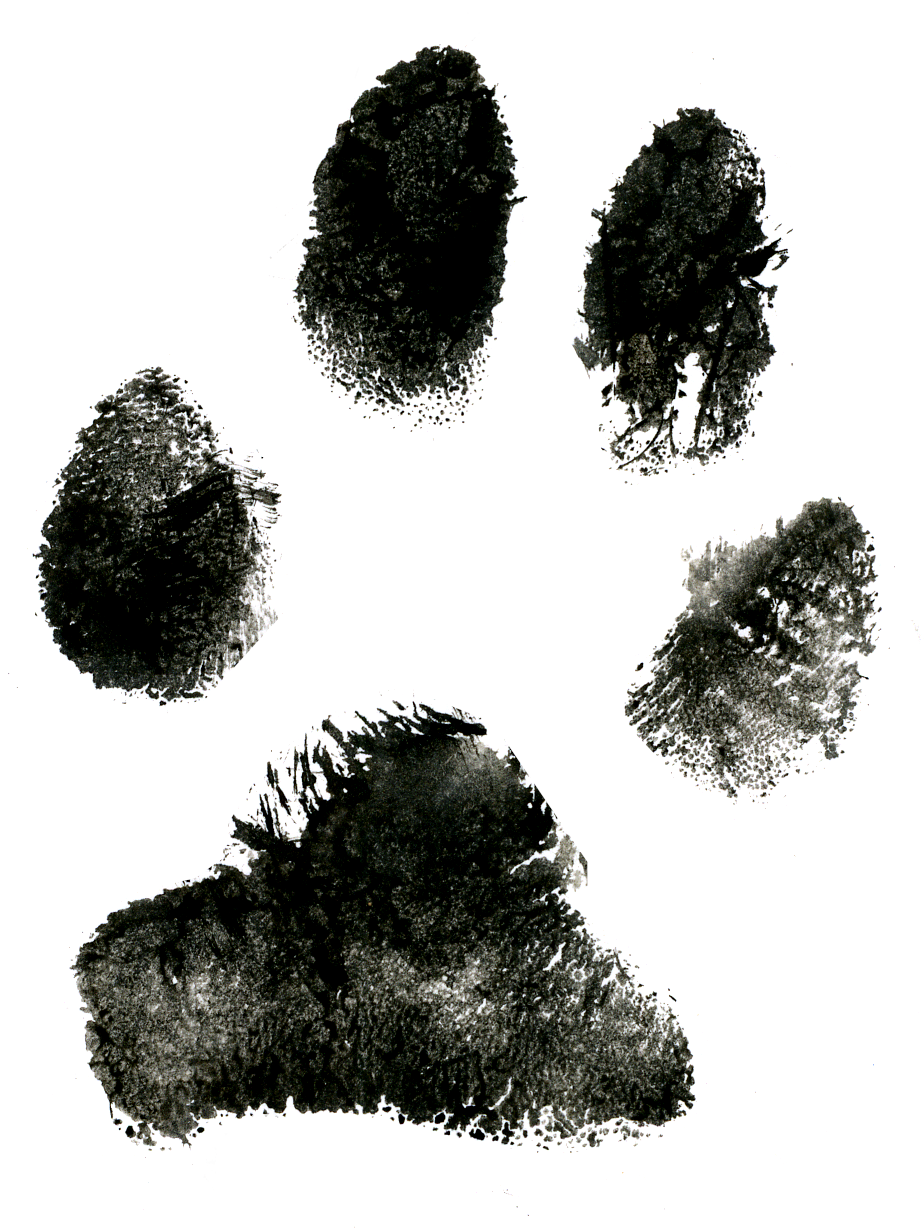
\includegraphics[width=0.5cm]{assets/zpaw.png}
  \end{center}
}

\newcommand\storydiv{
  \begin{center}
    \null
    \vfill
    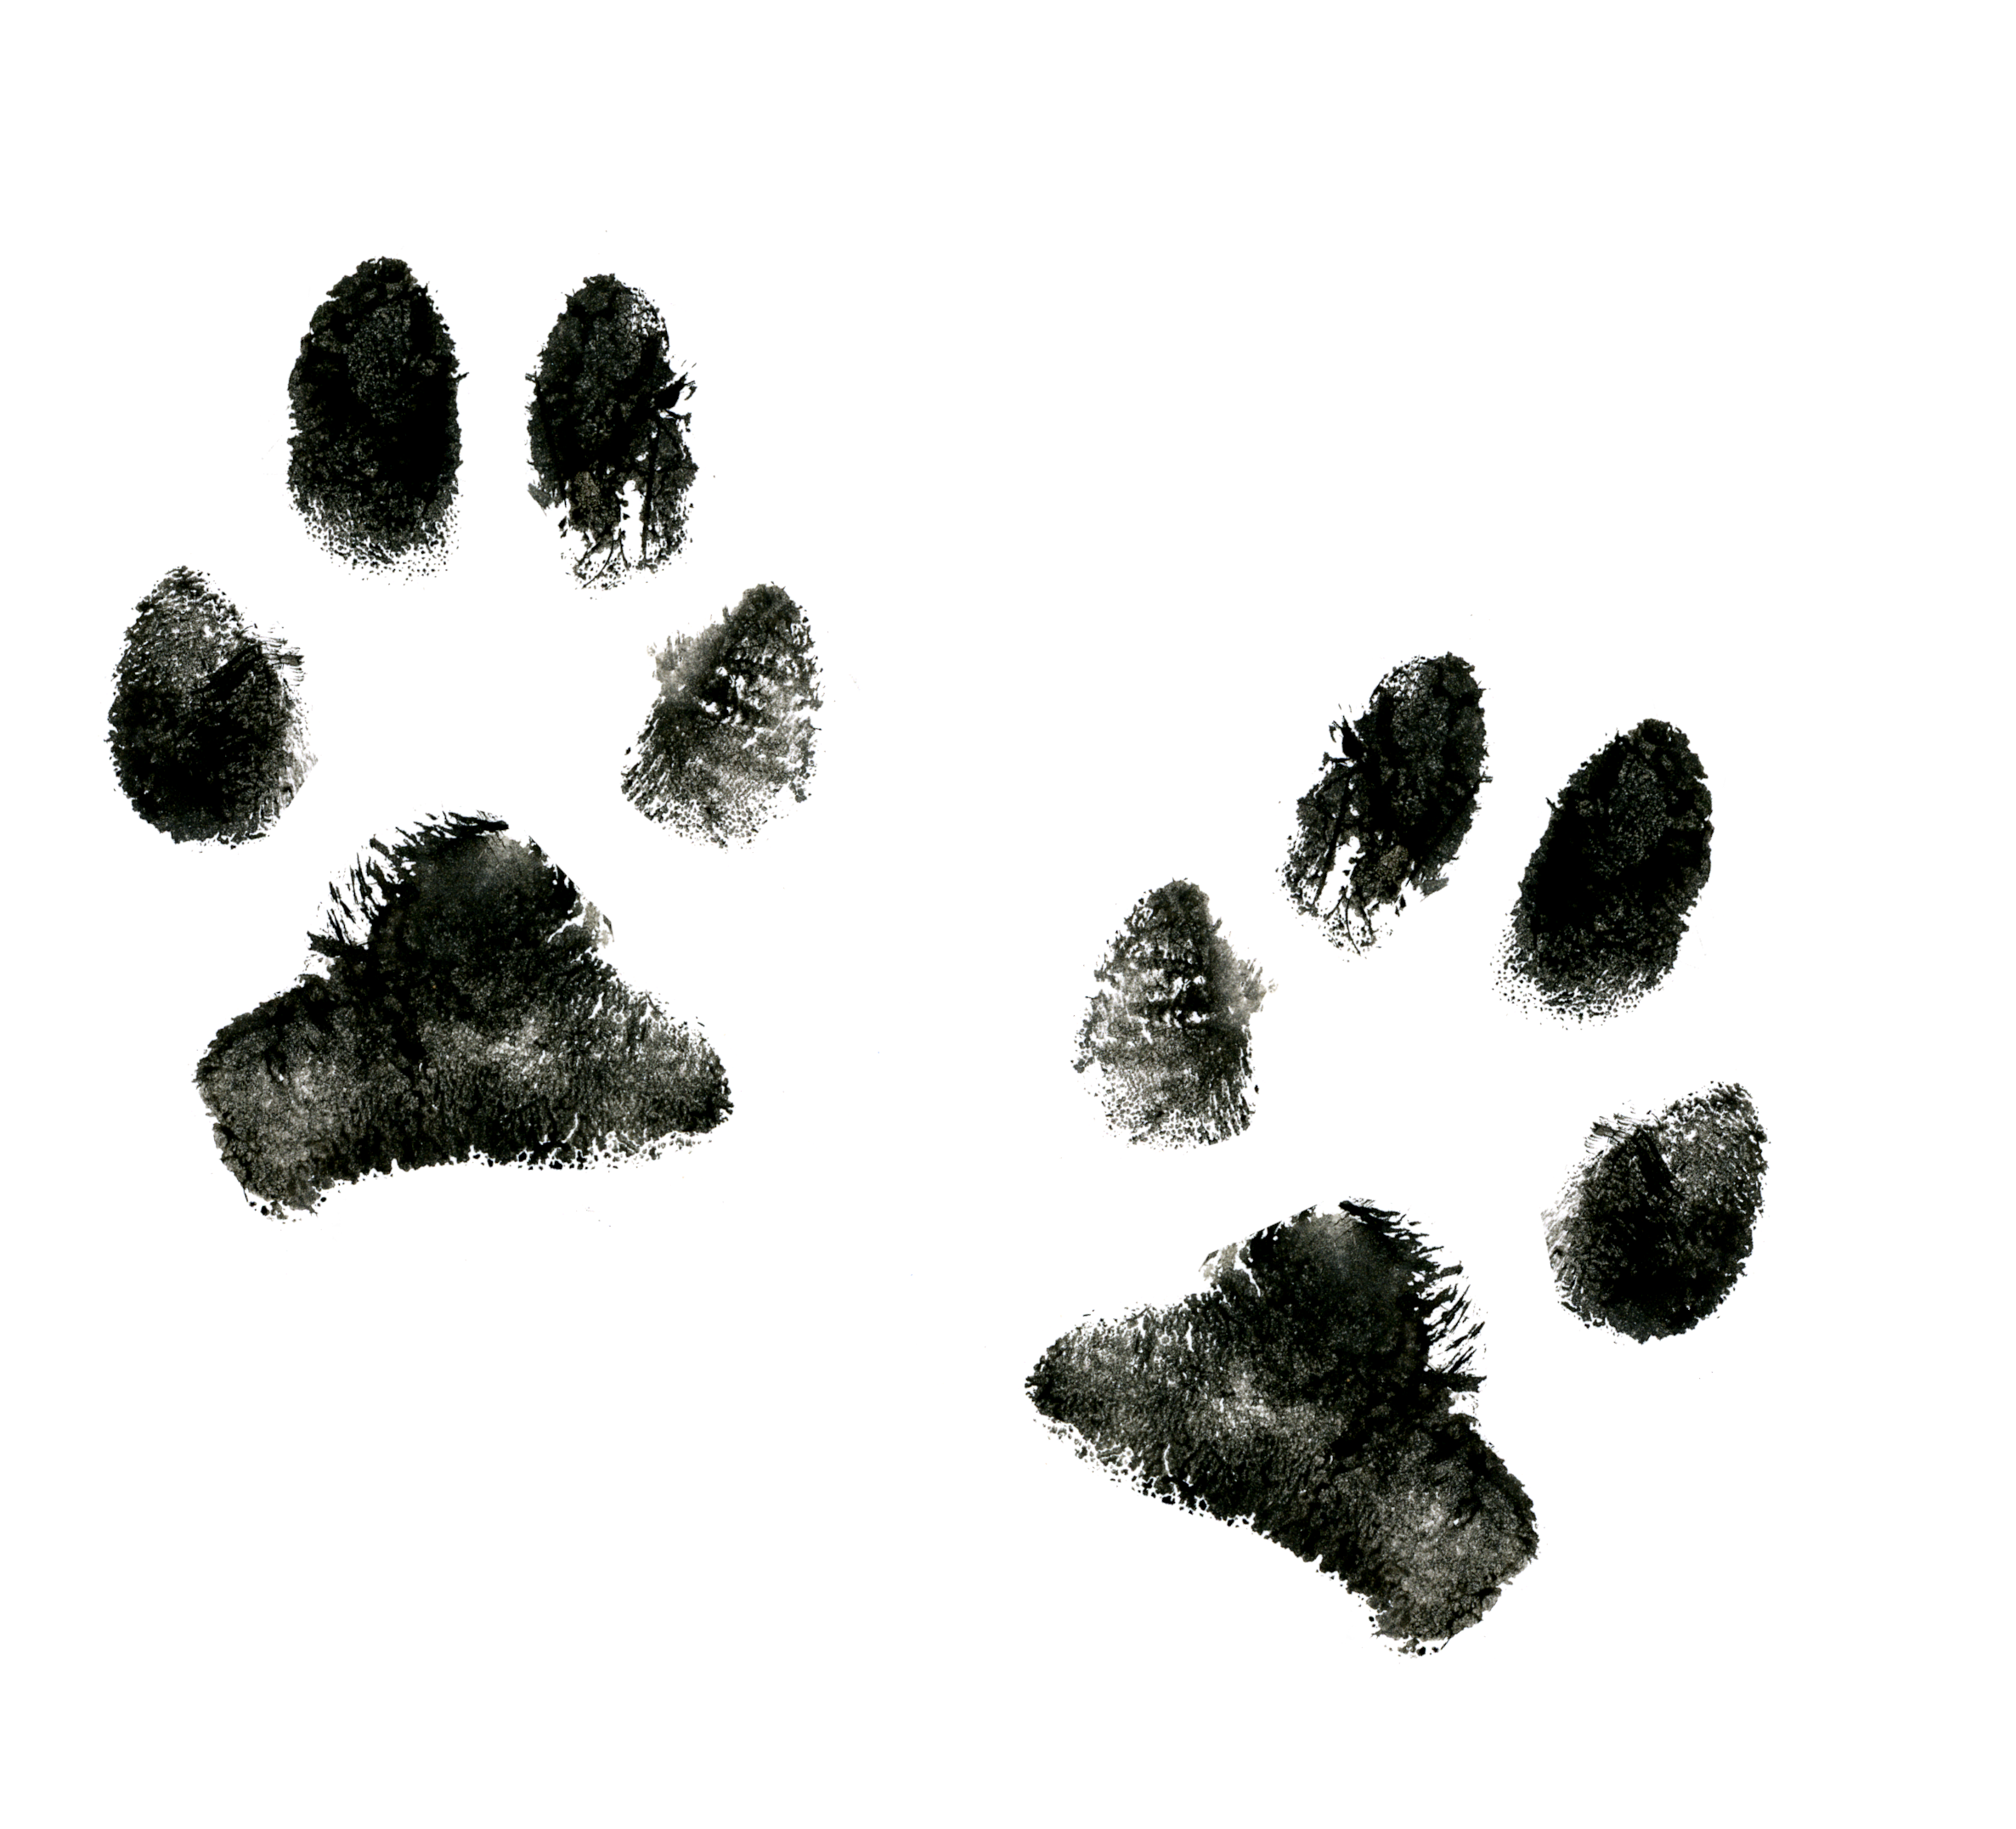
\includegraphics[width=1.7cm]{assets/2zpaw.png}
    \vfill
  \end{center}
}

\hyphenation{
\AuthorFirst
\AuthorLast
\Title
\Subtitle
}


\begin{document}
  \frontmatter

  \thispagestyle{empty}
\null
\vfill
\begin{center}
  \TitleFont\FullTitle
\end{center}
\vfill
\cleardoublepage


  \pagestyle{plain}

  \doublespacing

  \begin{flushright}
    \null
    \vfill
    {\Huge\DisplayFont Post.Self}

    \vfill

    {\Large\DisplayFont Madi{\kern-1.2pt}s{\kern-0.5pt}on Scott-Clar{\kern-0.4pt}y}
  \end{flushright}
  \thispagestyle{empty}

  \newpage

  \singlespacing
\thispagestyle{empty}
\begin{center}
    \noindent {\DisplayFont Also by Madison Scott-Clary}
    \TitleFamily

    \vspace{2ex}

    \emph{Arcana — A Tarot Anthology}, ed.

    \vspace{1ex}

    \emph{Rum and Coke — Three Short Stories from a Furry Convention}

    \vspace{1ex}

    \emph{Eigengrau — Poems 2015-2020}

    \vspace{1ex}

    \emph{ally}

    \vspace{2ex}
    
    \textbf{Post-Self}

    I. \emph{Qoheleth}

    II. \emph{Toledot}

    III. \emph{Nevi'im}

    IV. \emph{Mitzvot}

    \vspace{2ex}

    \textbf{Sawtooth}

    \emph{Restless Town}

    \emph{A Wildness of the Heart}

    \vspace{2em}

    Learn more at \emph{makyo.ink/publications}
\end{center}
\vfill
\singlespacing
{\small\parindent0pt\parskip5pt
\noindent Copyright \copyright\ 2020, Madison Scott-Clary. This work is licensed under the Creative Commons Attribution 4.0 International License. To view a copy of this license, visit \mbox{\emph{creativecommons.org/licenses/by/4.0/}} or send a letter to Creative Commons, PO Box 1866, Mountain View, CA

\vspace{1ex}

ISBN: \ISBN

\vspace{1ex}

\textit{Nevi'im}

\vspace{1ex}

Cover \copyright\ Iris Jay, 2022 --- irisjay.net

\vspace{1ex}

%\textit{This digital edition has been posted to Internet Archive and OpenLibrary by the author.}

\Edition\ Edition, \Year. All rights reserved.

\vspace{1ex}

This book uses the fonts Gentium Book Basic, {\DisplayFont Gotu} and {\TitleFont Linux Biolinum O} and was typeset with {\usefont{OT1}{cmr}{m}{n}\XeLaTeX}.

%Printed in the United States of America\\
%\EditionsList
}%\parindent0pt

\clearpage


  \tableofcontents*
  \newpage
  \null
  \cleardoublepage

  \onehalfspacing

  % \null

\vfill

\noindent \textbf{Content Warning:} These stories contain descriptions of sex and sexuality. \emph{How Many} contains explicit description of mental health issues. \emph{Again} contains drug use.

  \null
  \vfill
  \begin{quote}
    \emph{...and God will call the past to account.}

    --- Ecclesiastes 3:15
  \end{quote}
  \vfill

  \mainmatter

  \pagestyle{ourbook}
  % \input{content/01-chapter-one}
  % \clearpage
  % \input{content/02-chapter-two}
  \part{Torah}
  \markboth{Torah}{}
  \chapter*{RJ Brewser — 2112}

The theater purred. It hummed to itself. It stretched and reclined. It relaxed, unwound.

RJ and the room let out a soft, long-held breath together, feeling muscles and wires relax, nerves and current disentangle themselves, slowly, slowly.

``Alright, everyone. It's midnight, time to start packing up,'' Johansson was saying from down in the front row. ``Ross, we're short one. Can you start pulling together all of the mics? RJ will help you get them sorted.''

``Mm,'' RJ offered through the sound system. Ey was busy putting the theater to bed, and couldn't spare more than a meager few syllables to the rest of the cast and crew. ``Get a headset, Ross, so I don't have to talk through the speakers.''

Those speakers were signing off, going to bed one by one through RJ's gentle attentions. The virtual board set about the task of returning to neutral, all of the gain knobs orienting themselves, then all of the monitor knobs, the sliders, the whole system ticking as it cooled down, minus the channel ey'd need to keep open to Ross.

``Hey boss, got a headset. Where do you want me to start?''

``Grab the lead, first,'' RJ murmured. ``Then Sarah and Catherine, they've got the nice mics. They should have a tiny number painted on the costume side that matches up with their box. All of the boxes are stacked in the pit, by the front wall, you should be able to get them out in one load, though be careful taking them back.''

``Got it, heading down to the pit now.''

RJ left the channel open just in case, though the soft sounds of breathing and the occasional curse as Ross bumped his head on the pit cover were distracting, while ey set about going through eir notes with the dozy theater. The next night's rehearsal was the last one before they went live.

Ey knew the show better than most of the cast, em and the theater. The two had to learn everyone's lines, plus a few cues when ey'd have to take care not to pick up any of the sound effects. Gun-shots. Chairs scraping. A scuffle. The clap of heels on the matte black of the stage itself.

The theater's job was to simply work with RJ and the lighting crew, responding to their knowledge of what was going on in the play, while RJ and Caitlin's job, as sound and lights, was to respond to the stage manager's near encyclopedic knowledge of the play, her view of the house.

All sound was under RJ's jurisdiction. Cast and crew both: ey spent as much time managing communication between the hands, the manager, and emself and Caitlin as ey did maintaining the sound from the performers.

They were all as ghosts in this. Even the theater. Their job was one that should be totally invisible to the audience, because it would only become visible if they fucked up. No one wanted to fuck up. Even the theater seemed to feel a sense of pride in doing its job and doing it well.

RJ soothed the room with a gentle cooing and reluctantly started the process of pulling back. Ey closed the channel with Ross and put all of the headsets to bed last of all, before ey slipped back from the interface, blinking as ey adjusted to seeing the cavernous hall with eir own eyes as eir fingers slipped from the contact points and ey leaned back from the headrest.

Ey shook eir head to clear it and stood up, stretching, before ambling from the tech booth down the stairs towards the stage. Letting gravity carry eir lanky form down two steps at a time, feeling air against eir face, smelling the treble note of dust and conditioned air all added to the newborn feeling of pulling back.

Ross was down there standing still and staring at the floor, muttering agitated questions into the headset.

``Hey bud, I'm here. The house is sleeping now.''

Ross jumped, then looked embarrassed as he tugged the headset off his head. ``Sorry, was wondering where you'd gone. I just heard a beep.''

``Yep, signing off from above. Did you get all the mics gathered up?''

``Oh! Yeah, that's what I was trying to tell you. I wasn't sure what to do next.''

It only took a few minutes for RJ and Ross to get the last of the sound gear settled, gathering the headsets from all of the hands and socketing them into numbered chargers against the wall. Everything would sleep tight until the next night on sound's end.

Caitlin and Sarai, the stage manager, joined them and the rest of the hands. They sat on the edge of the pit cover, unwinding from the tenseness of rehearsal. The actors slowly got out of their dress to clump together on the stage, unwilling to leave their beloved platform just yet.

``Gather 'round, children'', a voice boomed from out in the darkened audience.

``Yes, Mister Johansson'', one of the actors recited back. Tired laughter.

``Good job, I think we're nearly there. Still, we need a bit more polish. No flubbed lines, and mostly relaxed, but Sarah, you gotta loosen up. It's not Shakespeare, you can chill out. Crew, you guys got a little sluggish toward the end. I know it's late, but so are our shows. Don't work yourselves too hard, but keep on top of things, okay?''

RJ, Sarai, and Caitlin murmured their assent.

``Tomorow night, back here at five.''

``Early,'' RJ murmured. ``How come?''

Johansson grinned wryly. ``There's a school production that winds up around then and I want you all back here to make sure we still have a theater.''

There was a bit more grumbling, but RJ knew they'd be there on time --- it wasn't too much of a stretch.

``Back to base, then. Get some rest tonight, and I'll catch you all tomorrow. Remember, you can drink tonight, but tomorrow night, \emph{Das is streng verboten}.''

The company laughed and started to disperse, the tech leads lingering on the pit cover for a little while longer as they worked on reorienting themselves to the real world. A world limited by two eyes, two ears, two hands.

Eventually, RJ made eir way out onto the chill of the street, pulling eir thin waterproof gloves on to keep the contacts on the middle joints of eir fingers clean and dry.

At midnight on a weekday, there wasn't too much going on. Folks visiting the pubs to catch up with their friends after work. Black cabs, night busses. By the time that midnight rolled around, those who were left were the harder drinkers.

The idea of a warm pub and one quick pint before heading home tugged at em, but the pull of home was much stronger than that of beer.

Ey trudged instead up to the northwest corner of Soho to Oxford Circus. Central line up to Benthal Green, walk the few blocks from there to eir flat. Stopped to pick up a take-away carton of curry and rice from one of the more trustworthy shops along the way.

Once home, ey slipped out of eir jacket and welcomed the warmth of eir little flat after the damp chill of London outside. Eir cat trotted up to em, twining around eir ankles. A little ginger thing of a few years that ey had rescued from a friend who was moving deeper into the city, she was the only one to share eir space with em after eir last flatmate had left for somewhere cheaper.

``Hey Prisca, let me put my shit down before I get you food.''

A meow followed em to the kitchen, where ey set eir take-away on the counter and scooped a cup of dry food into a fresh dish, setting it on the tile for the delicate cat.

Ey thumbed eir phone with the contacts on the thumb-pads of eir glove to start music playing. Some of the stuff that reminded em of eir dad to go along with the curry that reminded em of eir mom. Quiet, but present.

Dinner was no more or less exciting than usual. RJ ate alone at the kitchen table with the carton spread out before em, baring orange curry and the soggy samosa that had come with it. Ey left eir gloves on just to be sure --- no sense in having to clean eir contacts more than ey'd already need to after a long rehearsal.

Ey scooped the last of the curry into a little plastic container for the next day's lunch, promising emself that ey'd cook an additional pot of rice before heading out in the afternoon so ey'd have more calories to keep emself running. Clean up as easy as tossing the container into the compost bin along with all of the others. Cooking much more than rice was for times other than crunch.

The rig in the corner of eir bedroom was exerting subtle gravities on RJ. As ey ran through the motions of the post-recital evening --- eating, cleaning, storing leftovers, using the toilet --- eir orbits grew smaller and smaller. Eir gloves were itching. Ey could feel phantom breezes brushing past phantom fur. Phantom fur. Phantom ears. Phantom tail. Phantom realities teased around the edges of eir perception.

Ey finally allowed emelf to sit down at eir rig, relaxing into the familiar curves of the chair. Even with the draw so close to em, ey took eir time. Ey picked up Priscilla and stroked her smoothly from ears to tail a few times until she started purring up a storm, informing her that, in fact, she was the prettiest kitty.

\emph{Peel your gloves off one finger at a time,} ey thought. \emph{Relish the anticipation. Get caught up in it. Hell, let it linger.}

Cat settled into eir lap and curled into a small crescent, ey set about cleaning the contacts on eir hands with lint-free paper and rubbing alcohol. Those done, ey wiped down the headset, removing the negligible residue of sweat and skin oils that had collected there. Clean enough as is. Ey had recently replaced the soft, padded headrest where eir forehead would lay, held inches from the minuscule cameras that tracked eir face.

Eir gear was more elaborate than the stuff in the tech booth at work ey shared with Sarai and Caitlin, and ey had drained eir savings to acquire it. The rig, as well as the contacts on eir fingers, the nanoscale interferites --- the ones that took over eir optic and auditory nerves, and the electroparalytics to keep em from acting out in reality what took place online --- the NFC connections implanted just under eir hairline and their ramifying tendrils, all of that painful work down eir spine that helped em more fully experience the connection.

Connections and gear cleaned, RJ finally felt at ease enough to pop open the lid on eir rig. The screen, all but vestigial when ey was inside, still served its role during boot and login.

Ey quickly keyed in eir passphrase and then rested eir right hand on the curved pad, eir fingers finding familiar grooves that held eir hand in place. The connection from eir contacts the other half of eir two factors of authentication.

``Gonna head in, Prisca,'' ey murmured to eir cat, stroking the fingers of eir left hand over her ears, fingering the soft, velveteen folds until the cat shook her head away. Purrs nonetheless ratcheted up a notch. ``I'll be back in a bit.''

Ey set eir left hand into its cradle. Tilting eir head against the headrest, feeling the comforting touch of cool microfiber and the little twinge of recognition from the NFC controllers, ey nudged the button beneath eir thumb.

The rig went immersive. As RJ delved in, the soft hum of a cooling fan picked up to handle the waste heat of countless computations.

Ey could no longer hear it.

%%%%%
\chapter*{AwDae — 2112}

AwDae sat up in bed and slid to the edge of the mattress. Ey stretched languidly and let eir fur bristle from tip to tail, the latter bottle-brushing out. Ey shook emself to settle eir fur back down and yawned widely, slender pink tongue curling just shy of sharp incisors. A formality, to be sure, or perhaps a wordless mnemonic to finish the context-shift. The final step in a ritual.

Brushing eir fur down, ey stood and padded to the dresser in the corner of the room, pulling out a thin white cotton shirt with laces up the front and a simple navy sarong, which ey tied around eir waist. Countless hours examining some of the highest fashions out there on the 'net, and ey'd come to the conclusion that, in these times of excess, the understated said the most. It also interfered with the fur least, worked well with a tail --- a simple slit cut down the length of the sarong let that slip free --- and it was cheap. There was no shortage of ways to spend money, and AwDae had better things to buy with what was left after London rent.

Ey swiped eir paw from left to right atop the dresser, revealing a dimly glowing arsenal of personal belongings. It'd be a simple night out, so ey tucked a few vcards and a limited credit chip into a shoulder bag and hauled the strap over eir head, ears laying flat and out of the way.

From there, eir claws clacked against the glossy surface of the tport pad. Gauche as it was to appear and disappear where folks could see, ey kept eirs in a corner of the studio apartment rather than an alcove. The feeling of exposure and the jarring change of scenery was titillating, racy.

Ey stood straight on the pad and brushed eir paw from left to right, bringing up a list of recently used commands. Had ey left fingerprints online, there'd be a clear smudge over the entry: ey rarely did anything else on work nights.

\texttt{tport:\ The\ Crown\ Pub}

Tapped, and the obligatory click that went along with the change of scenery brought em to an alcove paneled in oak, lit by green-shaded lights hanging pendulously from a cord directly above em.

Ey blinked to adjust to the comparatively dim light. The pub, which largely followed the circadian rhythm of the British isles, was just as dark as it was for RJ, back in London-as-it-was, but eir perosnal sim lived in a perpetual eleven AM springtime.

Ey turned and stepped away from the pad, narrowly avoiding a slender weasel stumbling towards the alcove.

``See ya, Debarre,'' AwDae said, though it came out more like `Shee-a, Debaw' coming from the fox's narrow muzzle. Ey got a curt wave from the weasel done up all in black.

The fox shrugged and headed into the pub proper, eir nose twitching. The scents of the room which told em more of those present than simply scanning the crowd. One or two gawking entities with no scent property set --- tourists --- and the usual crowd of aromas. Friends, mostly. Acquaintances all, minus those tourists.

Ears perked at the distinct whiff of dandelions, something leftover from eir youth, and ey made a beeline towards one of the window tables, where the scent seemed to originate, skirting around bodies of diverse shape.

``Shacha.''

``Come on, fox, loosen your filters, won't you?'' Sasha laughed, scooting her chair back to stand up and lean in for a quick hug. AwDae slipped eir arms around the skunk's waist in turn and gave a squeeze, tail aswish.

``Lame,'' ey drawled, but dialed back the output filters on eir speech, letting something more closely resembling English pass. ``How you been, skunk?''

``Oh, you know, same old, same old.'' Sasha settled back into her chair and fiddled with a stack of vcards on the table, giving an outsized shrug. ``Been kind of boring in here over the last few days, so it's good to see you.''

The fox nodded, tugging eir shirt straight and moving over to the chair opposite the skunk, sliding into it easily and resting against the back.

``It's late there, isn't it?''

``Not too late. One something. Made good time home at least. Rehearsal ran late.''

Sasha laughed, ``You know, every time you talk about rehearsal and such, I think back to school. You hunched over the sound booth, you know? It's hard for me to picture you as having grown up and taken that up as a job.''

AwDae adopted a look of mock-despair. ``Is it? I went to uni just for it and everything. But hey, London ain't bad, I can't complain any.''

The skunk rolled her eyes and leaned forward onto her elbows, muzzle resting on obsidian paws. ``Tell me about it. You're missing out big time here in the 'burbs, dear. You could be teaching high school theater in any town along the central corridor, doing the same plays once every five years so no students repeat them. Truly a life of glamour.'' Sasha laughed as AwDae buried eir face in eir own paws with a groan. She continued, ``Seriously though, you just remind me a lot of school. Maybe it's 'cause of all of the ways you haven't grown up.''

``Please, Sasha.'' AwDae poked eir tongue out. ``If you bring up dating\ldots{}''

``Hey, sorry, just looking out for you, fox.''

``I'm plenty happy on my own, I can promise you that,'' ey countered.

``No, I get that,'' Sasha admitted, lowering her gaze. ``Not all it's turned out to be. Just got me thinking, is all.''

``Oh no, struck out again?''

Sasha shrugged, nodded, shrugged once more, fiddled with a vcard. Still no eye contact.

AwDae reached eir paws out to take one of her own, black fur on black fur nonetheless mismatched. Both had opted for mostly hand-like paws, but differences were evident on contact. Where Sasha's fur was an even, silky black marked by white stripes that were a little too sharp, a little too exact, AwDae had labored to construct a version of emself as a cross fox to exacting detail, down to the point where eir muzzle couldn't even form the two letters that made up eir name offline.

It brought to mind thoughts of honing versus forging. AwDae had honed emself to a finer and finder point while everyone else forged ahead. Always a way to be a better tech. Always a chance to become more vulpine online. Always a way to become better at what one already was.

Ey shook eir head to dislodge the rumination.

``I'm sorry, Sasha\ldots{}''

Sasha shrugged again, as though she might be able to drop the very idea of bad break-ups like an overloaded backpack. She gave the fox's paws a squeeze in her own. ``Men are dicks. I'd take a fox like you over any dickhead guy any day.''

AwDae smiled faintly, returned the squeeze. ``Sasha, you know it wouldn't--''

``No, I know. I just wish there were more guys out there like you.'' When AwDae stiffened in eir seat and looked away towards the window, Sasha splayed her ears and added quickly, ``Sorry fox. I keep putting my foot in it, don't I?''

``Sorry, no, you're fine.'' AwDae grinned apologetically. ``I should get a thicker skin, maybe. Stand up for myself. I spend night after night hiding in here, and even then, can't really assert myself any. I appreciate you trying, though.''

Sasha smiled cautiously and nodded. ``You came out like ten years ago, dear. I should still be doing better.''

AwDae's turn to shrug. ``It's hard to ask for that is all. Always has been.''

``I think that's what I meant earlier, that you haven't changed, despite all the ways you have. You haven't done like all the rest of us and grown up, gotten married, all that crap. You're still doing what you loved to do in school. You seem kind of frozen, kind of stuck --- in a few ways, even, though you're succeeding in others.''

AwDae nodded, rumination hanging in a cloud around em. So many ways the world had moved on without em\ldots{} After a moment, though, ey sat up straighter. ``Oh, speaking of frozen.''

``Debarre?''

The fox nodded.

``No news, yet. He's been trying to get in touch with the center that's taking care of Cicero, but the family's been getting in the way. They're fielding everything. They always sort of supported the relationship on the surface, you know, but never actually approved of it. Of them being together, I mean.''

``What? Really?'' The fox shook eir head, poking a claw at the table, before rubbing the spot with a paw pad. The sim was hardly immersive enough to waste cycles on letting claw dent tabletop. ``That's unfortunate. Not all that surprising, I guess, given what Cice said about his family. They at least confirmed that's what happened, though?''

``That's what these are,'' Sasha said, slipping the stack of vcards over to em. ``There's contact info for the family, and a few centers around there that work on implants, some hospitals. We're thinking that those might be the types of places where he wound up. There's also a card detailing his \texttt{laston} information.''

AwDae twisted the stack of cards around in front of em, leafing through slowly and taking in a few of the details that slid across eir fingertips. ``Mind if I make a copy?''

``Go ahead. It's a deck Debarre and I have been working on. Not complete, but I'll give you ACLs.''

``Mm. Debarre looked crushed. Is he doing alright?''

Sasha hesitated for a moment, caught in the middle of a gesture to grant copy rights on the cards. She shook her head, to which AwDae could only frown. She finished the gesture, and another set of vcards shuffled itself out from the original stack. Crisp black embossed on the creamy cotton-paper that AwDae preferred.

``I'll take a look, too. I can't do too much right now, I've got a--''

``I know, you've got a show coming up,'' Sasha laughed. ``Don't worry about it, dear. Debarre's working on it, I'm taking a look when I can, and I'm sure the weasel's got others helping him out besides us. No reason not to, either. We all liked Cicero.''

The two sat in silence. AwDae slid Sasha's cards back and fanned eirs in front of emself before shuffling them back into a stack and swiping above them, instructing eir rig to make a copy of the deck.

Ey lifted eir gaze away from the silence to scan the scents in the room once more. Now that it was starting to get on in the evening even in the Americas, the scentscape was changing. Some familiar scents, some unfamiliar, but most of them at least detailed, which told AwDae that the owners had put some thought into them. None, however, really jumped out at em.

More rumination. Rumination edging into drowsiness.

``Hey, Sasha, I gotta get going. I know I just got here, but I'm starting to crash hard.''

The skunk nodded and gave a little flick of her tail. ``No, it's alright. It's late there, and I know you've been in rehearsals for a while. Go get some sleep.''

Both stood up and exchanged another hug, AwDae breathing in that dandelion scent of eir friend. Memories of school, drowsy, dreamlike. Dandelions in the lawn. An impromptu picnic. Rubbing one of the flowers on the back of eir hand, leaving a yellow stain. Sasha explaining that the smell always reminded her of muffins.

``I'll see you later, skunk, yeah?''

``Take care of yourself, okay? No working too hard, slaving over a hot rig\ldots{}''

AwDae laughed and shook eir head. Ey gave the skunk one last squeeze before making eir way back through the crowd toward the alcove, already swiping eir command palette into view to head home.

%%%%%
\chapter*{Ioan Balan\#Tracker — 2305}

Ioan Balan awoke to an urgent message.

Ey didn't really like these, the sensorium messages. Ey liked paper messages. Ey mostly just liked paper. Ey was always accruing more. Paper and pens. Eir friends thought it creepy. Paper messages, or those rich messages that came attached to paper, played on its surface, or even messed with eir sensorium. To have one that just barged in on eir vision and endocrine system like this made em quite anxious. This one included a tiny jolt of adrenaline as an alert. Waking up with that jolt to have a partial sensory takeover just felt rude.

The benefit was that ey didn't have to get out of bed to deal with it.

The opacity on the message was turned up quite high, so that even in eir dark room, with eir eyes closed (and heart still pounding), ey could see the fox. A bipedal fox dressed quite sharply. It was sitting on a fairly plain wooden chair, situated in an empty room. The room had wood floors the same color as the chair, some very light wood, like hickory or pine. The walls were concrete where they weren't glass. Outside the glass was a sere shortgrass prairie, a cloudy day.

The combination of the fox's white fur, glistening and iridescent, combined with the room and landscape was all painfully pomo. Ey didn't consider eirself much of a pomophobe, but this was\ldots{}intense.

\emph{``Hi Mx Balan,''} the fox was saying. \emph{``I have a proposition for you.''}

Ioan grunted. The message was recorded, thank goodness. No interaction

\emph{``My name is Dear, Also, The Tree Was Felled, or just Dear, and I'm a member of the Ode clade. I'm an artist-''} Ioan rolled eir eyes. Ey could tell it didn't like the word. \emph{``-and performer. I'm not just telling you this to, ah, toot my own horn, I believe the phrase is, but just to underline the fact that I'm woefully unprepared for the situation at hand.''}

The fox smiled, looking tired. \emph{``I need some help finding someone,''} it continued. \emph{``Someone that doesn't want to be found. It's personally important, but also potentially damaging to the image of our entire clade.''}

Ioan furrowed eir brow.

\emph{``The person has information, a name, that ey have supposedly shared. We --- the other members of my clade and I --- don't precisely know if they actually did, unfortunately, we just have word from others close to the clade that someone knew and said The Name.''}

The fox shook it's head, ears flopping from side to side. \emph{``I'm sorry, I'm getting sidetracked by details. I try to be prepared for conversations and messages like this, but I'm a little worked up, excited, I guess. Can we meet?''} It listed some coordinates. \emph{``Even if only to talk. Even if you're not interested, I'd still like to meet you. You seem neat.''}

The message ended.

Ioan lay in bed, thinking. It was still about an hour before ey had to get up, and ey was loath to start the day before ey had to. Ey tried eir best to sleep for another ten minutes, at least, but eir mind kept slipping back to Dear's request.

\emph{Why me?} ey asked the backs of eir closed eyelids. \emph{Why hire a writer who fancied eirself a historian as a PI?}

With still a half hour to go before ey had to be up, Ioan slipped out of bed, stood, and stretched. The least ey could do was get a shower and some coffee. If there were any reason that the founders of the system had included sensoria in the works it must have been for those.

Those done and clothes donned --- ey knew ey could never out-natty the fox, so the usual faux-academia garb it was --- ey penned Dear a short note with a time. If it was day in that sim, or even late afternoon, it should get the note before dinner or bed.

\emph{Besides,} ey thought. \emph{Maybe it will get the fox to start sending notes this way in the future.}

No luck. Less than thirty seconds later, Ioan received a sensorium ping of acknowledgement, and a shiver up eir spine to go along with it.

Ey forked and sent \#c1494bf out to the meeting. Meanwhile, ey'd get some food.

%%%%%
\chapter*{RJ Brewser — 2112}

RJ slid eir hands from the pads and leaned back from the headrest, letting out a full-fledged yawn. The sound and motion startled Priscilla across the room. Ey levered emself up out of eir seat and trudged over toward the still-purring cat, stroking over her ears when she bunted her head up against eir hand

Eir mind foundered in a slurry of work, of Cicero's disappearance, of school with Sasha, of honing versus forging.

``I'm wiped, Prisca,'' ey informed the cat.

Priscilla purred louder.

Smiling, ey peeled eir shirt off over eir head and slipped out of eir jeans. Tomorrow's rehearsal would mean full dress for everyone and makeup for the actors. Ey'd have to make sure eir suit was clean. Should ey iron it? Maybe ey should iron it. Later. For now, as it neared two, ey focused on making sure the door was locked and the lights were out before stumbling over to bed.

Ey flipped the screen down on eir rig to signal for it to go to sleep and wandered over to eir bed. There seemed to be no shaking Sasha and all of her talk of high school, gone these last eight years now, out of eir head. Even as ey climbed into eir narrow bed and burrowed beneath the covers against the chill of the night, ey was replaying memories from school. Scenes from the US. A worn out film, dim and scattershot.

Honing and forging, honing and forging.

Ey and Sasha had tried dating early on. After a few weeks of it not going anywhere, they had both admitted that they had felt pressured into having a relationship, rather than actually wanting one. Good boys and girls fell in love with other good boys and girls, right? Pretended they didn't have sex. Went out to the movies.

The relationship petered out, rather than ending in some climactic fashion. They had continued the trend of going to movies, and later to live performances. They had never lost touch, at least.

Sasha had gone on to have a string of other relationships, some earnest and some not, some more intense than others --- a string that remained unbroken, if tonight's conversation was any clue --- but RJ had stopped there.

The intensity social pressure to date throughout high school was equaled only by RJ's total apathy toward the whole scene. Apathy or, often, antipathy. Ey'd felt the occasional twinge of romantic attraction, perhaps, but the expectation of sex that went along with the process so put em off that ey had instead buried emself in work.

Ey did well in some courses and not in others, but in the subjects that ey enjoyed, ey dumped all of eir effort. Huge gusts of energy that drove em forward.

Ey had started early on in working the school's older sound board in the theater Ey ran plays. Ey ran concerts. Ey ran assemblies and lectures and conferences, quickly earning the trust of the other tech crew and the staff and faculty. And then ey gained leadership. Prestige.

The various computer classes had captivated em as well, and for eir sixteenth birthday, eir parents had surprised em with the implants needed for full interfacing with a rig. Or, well, ``surprised'': eir father was an engineer and eir mother a fairly forward-thinking person, and they had promised em the procedure before university.

Honing and forging, honing and forging.

It was a straightforward procedure in an outpatient office, self-guided implants largely installing themselves. The worst had been the itching. It was bearable on eir hands and along eir spine, where the implants and exocortex breached the surface of eir skin, because at least ey could scratch, though ey had been cautioned not to. The NFC pads in eir forehead and the interferites embedded deeper --- far, far deeper --- led to an itch that no scratching would ever reach.

From there, sound and the interface had taken up all of eir energy, leaving little time to worry about any social stigma that went along with an aversion to romance. Ey was simply the nerdy sound kid who knew more about computers than the teachers.

It hadn't always been fun, of course, but by the ey quickly learned that the more ey put into the task, the more ey got out of it.

That ey had found furry in high school seemed almost a natural progression. Working and improving at the art of interfacing in a way that felt natural to em came just as natural to others on the 'net. Ey moved effortlessly through the Crown Pub and a few other choice spaces, slowly crafting the primary persona that ey used when interacting with others, the cross fox known as AwDae.

It was then that ey and Sasha had really started connecting, for it was her that introduced em to the community. They started hanging out more, talking more, building a network of friends together. Where dating hadn't worked out for them, friendship grew in depth and breadth.

Honing and forging, honing and forging.

The forging of the virtual theater environment had culminated in a scholarship at a big name university out on the east coast. Immersive interactive theater technology. Forging into honing.

It meant leaving Sasha and a few other close friends behind along with eir family, but it also meant that ey would be at the forefront of a new tech. Something used in production. Films and live work, too.

The field had been so new that eir own studies at the university helped fuel the change in theater tech work. Eir dissertation, what was meant to be eir capstone project, was published and spread. Theaters around the world were using immersive tech.

Ey had continued to work at the university for a while. It was one of the few places around with both a theater and the hardware to back it up. Ey had considered continuing eir studies, but the draw of the theater was too heady, too alluring. Academia spelled a life of forging, work one of honing. Why deny one's base nature?

Honing and forging, honing and forging.

The call from London came less than a year after ey graduated. Would ey like to help start a tech-savvy theater group in town? The pay would be slow to start, but the troupe had a loose collection of apartments on the East End. Ey would have full run of the sound department. When could ey start?

Eir parents had needed convincing. They were pleased, to be sure, but they London, so far away! Still in the western bloc, but so far.

Ey made eir promises that ey'd come and visit every year, and packed eir bags.

Burying emself deeper into the covers and the mattress, leaving enough room for Priscilla to join em later, RJ's thoughts alighted on Cicero, on the lost.

Losing Cicero had been a shock. A disappearance, at first, and then it went on. Debarre hollering one night after getting in touch with Cice's family. Lost, lost, he was lost.

Getting lost was rare. Vanishingly so, even, with perhaps two dozen cases. Still, among those who were counted among the lost, all were heavy interfacers. It was a risk, everyone had assumed, just as was travel. Call it occupational hazard. Something could always happen. Something could always go wrong.

To lose someone so close, though, hit hard.

It was a reminder of just how much ey relied on the integration tech, not only for work, but for a large part of eir social life. Ey enjoyed the company of the troupe just fine. Troupe pub trips were a weekly affair, but eir heart lay among eir friends on the 'net. Eir friends being on the 'net meant more interfacing, and more interfacing meant more risk.

Eir tech was truly immersive, after all. It was a dissolution of the body. Disembodied in the truest sense.

It was becoming the room. It was a new sensory experience. No limbs, no torso, no face or eyes or ears. Or maybe all ears: ey became the room, feeling the way sound echoed or didn't, knowing the limits of the speakers in a deeply physical way. Mics peppering the walls a new sensory input. The wires nerves. The speakers muscles to flex. Instincts, reactions, and actions responding to whole systems of stimuli.

Perhaps that was why ey felt so at risk. They all were, of course, but to dissolve one's concept of a body at work, and then come home to warp the very same concept into that of a fox --- no, a finely wrought amalgam of fox and self --- felt perilously close to being lost, sometimes.

Honing and forging, honing and forging. Risk and reward.

Ey slept.

%%%%%
\chapter*{Dr Carter Ramirez — 2112}

Carter rubbed her face into her hands, ground her palms against her eyes until she saw stars, slicked her hands back over her head in a vain attempt to wrangle fly-away hair. It had been in a neat bun this morning.

She wasn't the last one left in the lab, but it had reached that point of the night where collaboration had stopped and everyone was butting their head against their own individual problems, toiling in silence. She folded her rig's screen down, sending it to sleep, socketing her tablet in next to it to charge.

It had also clearly reached the point of the night where she wouldn't be getting anything else done.

She felt out of her league. Everyone did, here on her team, but that didn't stop the fact from wearing on her. It's not that there wasn't any support from on high. There was. It's not that there wasn't anyone else trying. There definitely was.

It's that no one seemed to take it all that seriously. It was like addiction, or plane crashes, or suicide. Something to look at, to study long enough to say ``Ah, \emph{this} is happening now,'' and then set aside. Conversation-piece science.

People admitted that the phenomenon was there, but only in as much as it didn't affect that many people. A simple number to point to. See how small?

It was as though the brains of the Lost were just\ldots{}elsewhere. Just dreaming on some level. There was no sense to it, though. No rhyme or reason to why such a thing would happen to the patient. Some of her team were pulling together all of the facts about the population that they could, from demographics to physical stature, searching for clues in the rig and the 'net itself. The neuroscientists were digging into what was going on within the brain, and what few scans they had from before someone had gotten lost. Their two pet lawyers --- just law students on internship, both also versed in stats --- were digging into the legal status of the lost as well as writing queries to procure patient medical histories.

And Carter was supposed to tie it together.

Or, that was her stated goal. The university medical center had only grudgingly provided space and funding for the project. An attempt to win some much-needed kudos, she suspected. Still, she was beginning to doubt just how much the UMC wanted her to succeed.

There had been an initial dataset dumped on her team, and a slow trickle as new cases came in, but it all felt so carefully curated. As manager, she had been met with hurdle after hurdle as soon as she started to venture beyond that. Colleagues assured her that all projects worked this way, but it was as though the advisory board had given her all the data that it was willing to give, and any more might\ldots{}what? Put those kudos at risk?

Carter stood, stretched her back, winced. ``Sorry, Sanders. I'm shattered. Catch you in the morning?''

``Mm,'' he replied. The interruption seemed to him of his physicality. He rubbed at his eyes and stretched his arms out, alternating between clenching his long fingers into fists and flexing them out wide. ``Sounds good, Ramirez. Catch you then.''

Carter gathered up her coat and her messenger bag, taking one last look around the lab, counting heads to see who would be staying later than her. Not too many. Sanders, one or two of his neuroscientists.

She swiped her way out of the wing and signed out at the front desk before making her way out into the night, bundling up in her coat.

At home, she scavenged a few pieces of salami stacked onto a couple of crackers, enough to keep her empty stomach from complaining through the night, and crumpled onto the couch in the shared living room. She left the lights off so that she wouldn't bother her flatmates. Or so she told herself. In truth, the darkness felt good. She could keep her eyes open and not be greeted with a tablet, a screen, a sim.

She sat long after finishing her snack, listening to her flatmates sleep, the sounds of the road outside, her own breathing. Sat, thinking in the dark of all the administrivia on tomorrow's docket.

Eventually, finding herself at as much of a dead end as she had at work, Carter ambled off to her room, changed from her work clothes into a comfortable pair of lounge pants and a night shirt, and crawled into bed.

%%%%%
\chapter*{Ioan Balan\#c1494bf — 2305}

\noindent Ioan\#c1494bf found emself about twenty meters in front of the squat house. It was just as postmodern on the outside as it had appeared on the inside: a concrete block, a thick wrap-around patio covered by cantilevered eaves, floor to ceiling glass for walls. Ey wouldn't be surprised if the far side of the buiding --- ey couldn't see it very well, with the slope of the shortgrass-prairie it was on --- jutted out at some crazy angle.

Smiling ruefully, ey walked up toward the house.

A soft tone, a vibraphone struck with a soft mallet, sounded inside and outside of the house as soon as ey'd passed the barrier between grass and patio. Ey stood on the patio, waiting to be either admitted or greeted.

A shadow of a person, human, peeked out through the glass at em, gave a pleasant wave, and hollered through the glass, ``Ioan! Hi! I'll grab Dear.''

Before the person could do so, Dear came padding softly from around the side of the house, looking slightly more collected than it had during the message.

\emph{``Ioan,''} it said, smiling and offering a paw in greeting. Ioan wasn't sure how ey knew when a fox was smiling, but it was definitely a smile. \emph{``Thank you for coming on such short notice. Sorry for the urgent message, I just need to find someone to help out rather soon.''}

Ioan\#c1494bf took the offered paw and bowed. ``Of course, Dear.'' Ey realized how strange it was to call someone a term of endearment as a name. ``May we have a seat? I've just woken up and am still figuring out how to stand.''

Dear grinned and nodded, gesturing cordially with its paw around the side of the building from where it had come, leading the writer around and through a door in the glass.

The interior of the house was as ey had seen, though as they moved through the space where the message had been recorded (a gallery, Ioan noticed) and deeper into the house, things warmed up a little. The concrete walls were softened by hangings, and the furniture was unexpectedly plush, rather than of the firm-cushioned, straight-lined variety ey had expected. Fox and writer settled for an L-shaped couch, sitting facing each other across the bend.

After a moment's hesitation, Ioan began, ``I must apologize, Dear. I'm not sure that you have quite the right person. I'm not really a detective, wouldn't know the first way of finding the one you spoke of.''

Dear shook it's head, \emph{``I'm pretty sure you're the right person. I'm not really looking for a detective, per se. There's enough of those in the Ode clade. They'll suss out the whens and wheres.''}

``Then what-''

\emph{``There's a few kinds of people in the world, Ioan.''} The fox said, voice low and calm. \emph{"There's forgers and honers, of course. Forgers build a thing and plow ahead, and honers settle on a thing and perfect it. Artists generally fall into these classes: prolific and unfruitful artists, respectively.}

\emph{``But you're not an artist. You write, yes, but that's ancillary to what you do. A side effect. There are some other types of people out there, too: catalogers, feelers, experiencers.''} Dear shrugged, \emph{``For its own reasons, the clade needs someone to experience this. There's a lot of history in this, a lot that we've forgotten, a lot that we're trying to remember, maybe some that we're trying to forget. I want you to help figure out the history and story of this.''}

``An amanuensis,'' Ioan said.

Dear brightened, its ears perking. \emph{``Precisely. And what a delightful word, too.''}

Ioan grinned, ``That's good, then. This is very much more my arena. I'll keep this instance around and keep \#tracker up to date.''

The fox nodded and looked up, smiling as it's partner came in with three thick-walled, wide-brimmed mugs of coffee, setting two of them down on the corner of the table near Ioan and the fox. ``Heard you were tired,'' they said, walking off with their own mug.

Dear watched them go.

``Your partner?'' Ioan asked, feeling that a moment of chitchat was necessary. Ey grabbed eir mug eagerly. It smelled quite good.

The fox nodded, picked up it's mug as well and leaned back into the cushions of the couch, slouching. \emph{``Mmhm. Finally decided to explore relationships,''} it said. \emph{``They accuse me of treating it like an art project''}

Ioan grinned. ``Well, are you a forger or a honer of relationships?''

Dear rolled its eyes, said, \emph{``Touché. I'm trying to be a honer, with this one. For a long while, I forked to create lasting relationships. Gets lonely, though. It was like being turned down every time. At least from my --- this instance's --- point of view.''}

Ioan felt they were getting a little too deep for having just met, so ey steered the conversation in a tangential direction. ``You fork quite often, then?''

\emph{``Yeah, Dispersionista through and through. Or maybe profligate tracker, as sometimes I don't have the option to let instances linger.''} Something seemed to occur to it, and the fox sat up again. \emph{``Speaking of, do you know much about the Ode clade?''}

Ioan shook eir head, sipped eir coffee. It \emph{was} good.

\emph{``It's an old clade. One of the oldest on the system. Our founder, Michel Hadje, uploaded basically as soon as he could, and quickly became one of the, er, loudest voices on the system. He campaigned for sensoria to be included.''}

``I've heard of Michel!'' Ioan sat up straighter. ``Usually in the context of the founders.''

Dear nodded.

``So what is Ode, then? His old username?''

\emph{``No, a poem,''} Dear laughed.

``Oh! Oh, of course. So Michel wrote this poem\ldots{}''

\emph{``No, not actually. Michel had a friend, a good friend, who wrote the poem.''} Dear said, speaking more slowly now, sounding less rehearsed. \emph{``When the friend died, Michel memorized the poem. All us up-tree instances do our best to keep it memorized as well. Really memorized, too, in the forefront part of our head, up where we think about it, not stored in some exocortex.''}

``Is that where your names come from?''

\emph{``Mmhm. Each of us is named after a line in the poem. I'm Dear, Also, The Tree That Was Felled, and my first long-lived fork is Which Offered Heat And Warmth Through Fire. My immediate down-tree fork is Dear The Wheat And Rye Under The Stars.''}

Dear splayed its ears, grinning sheepishly, \emph{``It's not actually a very good poem, I must admit. Michel thought so from the beginning, too. His friend, though, when they died, when they killed themselves, it really tore him up. We all still think of them often.''}

Ioan nodded, ``It must be quite long, then.''

\emph{``It's only about a hundred lines, divided into ten stanzas. There are only ever ten branches as direct ancestors of Michel, and each branch only ever has ten long-lived up-tree instances. We may be Dispersionistas, but we're a small clade.''}

``And the poet? Who are they?''

Dear bristled, then mastered its instincts. \emph{``That's The Name that we don't share. The information that someone supposedly did share. Someone of the clade or close enough to it to know.''}

Ioan's mind swirled, confused at the fox's reaction, the concept of not sharing a name that was clearly important. ``I see,'' ey said into eir coffee, covering eir confusion. ``So you'd like me to help in finding this person and act as amanuensis along the way?''

Nodding, Dear held out its paw once more. \emph{``If you'd be willing, that is. We'd be glad to have you aboard.''}

Ey was already sold, Ioan knew, but all the same, ey took a moment longer to consider the ramifications of the job.

Ey shrugged, reached out and shook the fox's paw. Dear grinned, shook back.

\emph{``Excellent. I've shared just about all I have to share on the topic for now, though as we get updates, I'll pass them on to you.''} Dear leaned back into the couch once more, \emph{``For now, stay. Finish your coffee, at least, though feel free to putter around for a while. Or just stay here. We've got an apartment on the side of the house. I've already talked with-''} it said it's partner's name, Ioan didn't quite catch it \emph{``-about it.''}

Ioan nodded, ``Thank you. I think I'll head home in a bit and sync up with myself, and start the research plan. Do you have any suggested avenues I should start down?''

\emph{``Of course,''} Dear smiled. \emph{``As for research, dig a bit more into the Ode clade for now, probably. when I send you updates, maybe those will lead to different topics.''} The smile turned into a sly grin. \emph{``I know you're not a big fan of sensorium messages, but as that's how the clade communicates --- those of us who do, at least --- I regret to say that you'll be getting quite a bit more.''}

Ioan gave eir best polite smile.

%%%%%
\chapter*{RJ Brewser — 2112}

RJ allowed emself to sleep in until near eleven that morning. Last night of dress rehearsal, might as well be well-rested.

Many other members of the troupe held part time jobs during the day, and ey ran a small consulting business of eir own. The more industries that dove into immersive tech, the more eir expertise was worth. Even so, with all that ey did, ey made enough to not have to worry about holding down more than the one full-time gig.

As it was, on days when ey had nighttime rehearsals, ey felt no compunctions about sleeping in. Nothing to be up for, only the 'net to keep them occupied in the mornings, little enough need to get moving.

It was Priscilla who eventually succeeded in waking em, butting her head against eir cheek and purring obscenely. The more insistent the cat became, the less able ey was to ignore her intrusions on eir admittedly banal dreams.

Fine. Trudge out of bed. Refill cat's water and food. Give the requisite morning pets to keep her happy. Scoop the litter box. Make self a pot of tea. Tea to shake the grogginess.

Ey sat at the tiny kitchen table, sipping from eir oversized mug and watching the late morning traffic from their window. Mostly business traffic, with the occasional mother with child in tow. Black cabs. Scooters. Bikes.

By the time ey had finished eir first mug of tea, RJ had woken up enough to start on the prowl. As with the night before, ey made sure that everything was in order before touching eir rig. Ey'd taken care of the cat, but ey still needed to eat, emself. So, remembering eir promise, ey set about making a small pot of rice. Fifteen minutes to cook, plenty enough time to finish another mug of tea.

RJ left most of the rice cooling in the pot and took for emself a small bowl of rice and leftover curry. The process of swiping eir hand over the controls of the stove had reminded em of the deck that Sasha had shared last night. There was no reason to think that some random person in London would have much to offer in the case of another person ey had never met getting lost. No reason not to try, though. Maybe there was something, some small insight that ey had that, which, when pooled with those of others, which would help in some way.

So many maybes. So many mights and perhapses.

Empty bowl in sink. Third and final cup of tea in the thick-walled mug. Good enough. Ey allowed emself to settle before eir rig at last.

As before, ey keyed in the password and rested eir hand onto the cradle for the two-factor. However, instead of delving in as ey had last night, ey flipped up the monitor and pulled the keyboard closer, swinging the hand rests to the side and the headrest up and out of the way. No need to go immersive, with work like this. Ey could just as easily work as a fox, of course, but it was so easy to lose track of time in there, and the night's rehearsal mustn't be forgotten.

``Let's see,'' ey murmured, taking a sip of tea before setting the mug down

Ey called up Sasha's deck.

\begin{longtable}[]{@{}c@{}}
\toprule
\endhead
Cicero Lost Nov 2108\tabularnewline
Priv eyes only\tabularnewline
See Debarre for ACLs\tabularnewline
\bottomrule
\end{longtable}

\begin{longtable}[]{@{}c@{}}
\toprule
\endhead
Dr.~Carter Ramirez\tabularnewline
specialist in lost\tabularnewline
so. London\tabularnewline
\bottomrule
\end{longtable}

\begin{longtable}[]{@{}c@{}}
\toprule
\endhead
Mr/Mrs.~Jackson\tabularnewline
parents, can't get much more\tabularnewline
dad in govt, mother stays home\tabularnewline
\bottomrule
\end{longtable}

And on it went for nearly a dozen cards. Each had its own cover embossed with a few lines of type, and each contained upwards of a gig of information culled from various sources, doubtless of varied quality.

RJ flipped through each, gleaning what ey could from a quick scan, before collapsing the deck once more and sitting back to think. Nothing in there seemed new. Nothing out of place. Ey had only received the deck last night, and yet nothing felt like it had been revealed, uncovered.

Ey had heard of the lost before, and the name Ramirez was commonly tied with the hundred or so cases that had cropped up over the years. The family\ldots{}no, nothing to be gained there, at least not that had already been tried by Debarre. And again, there was the problem of being a random nobody in the UK: no one known, no one with power.

None of the rest of the cards carried any real significance to em.

If there was anything RJ was going to add to the conversation, it would be through eir connection to Cicero. Something ey knew, something the two had shared.

A small notification slid down from the top of eir monitor, covering the upper right corner of the screen.

\begin{quote}
\textbf{D --- D --- R}

Voting begins in \emph{5} minutes on \emph{referrendum 238ac9b8}:

Summary: \emph{Tariffs on importation of goods from the Russian Bloc\ldots{}}

Cost: 1,000

Bounty: 280,000
\end{quote}

RJ reached to swipe the notification away. Ey had very little stake in the uncomfortable alliance between Western Federation and Russian Bloc. Could care less, honestly, about taxes on things that ey'd never buy. Then something clicked within em, and ey halted eir motion.

\emph{Cicero.}

Ey hastily shuffled back through the \emph{Cicero Lost} deck until coming up with the `recent net activity' card and pulled up the contents. It took a few moments to remember how to sort tabular data --- database classes in high school, so long ago --- but eventually, ey got the table sorted around the activity type. Ey scrolled rapidly through the list until ey got to the list of Direct Democracy Representative entries.

There was the connection. The one thing that RJ and Cicero had was their arguments over politics. Not just politics, but the worthiness of the current political system in all of its facets. Arguments upon arguments upon arguments, cross fox and tabby cat with their ceaseless arguments in the Crown Pub.

RJ was firmly on the left, but ey felt the representative democracy combined with the DDR was a pretty good system. It was fine. It worked.

Cicero, however, seemed to waver between socialism and anarchy, depending on factors such as how much he had had to drink and how angry he was at the most recent vote.

\emph{I certainly can't see broad shifts going my way,} he had slurred on more than one occasion. \emph{Least I can vote. Vote on every damn thing that comes my way.}

Ey made sure syncing was turned on across all copies of the deck before snipping those rows out of the activity table into a card of their own:

\begin{longtable}[]{@{}c@{}}
\toprule
\endhead
DDR votes\tabularnewline
todo: process by record\tabularnewline
1 month, 835 votes (!)\tabularnewline
\bottomrule
\end{longtable}

The icon in the upper left of the screen showing the deck twirled gracefully to show the sync.

Cicero had voted precisely how he had talked. On the surface, he was no different than any other leftist socialist on the DDR.

Along with the ability to vote on issues directly came the ability to comment --- for a price. DDR votes didn't cost money, but they did cost credit. Up to 1,000 per. Credit gained by voting on cheaper issues, beginning with a few freebies in the tutorial.

What Cicero's records showed was that he was wealthy. Incredibly wealthy. RJ had a few million DDR credits banked away in case a high value issue that ey felt strongly about cropped so that ey could make a comment. Unlike voting, commenting could cost upwards of five million credits. And one could buy their way to influence by flooding issues with comments.

Cicero's wealth surpassed RJ's at least a hundred times over, if not more. For someone to be as active in commenting as ey knew the cat to be and still have that much in credits stored up showed a dedication to following politics that was just barely hinted at by those tispy rants. Cicero was well connected, well read, and, most importantly, a key political figure on the DDR comment sections to an extent that none of the Crown regulars had ever expected.

RJ sat back in silence for a few moments before muttering, ``Well, shit. Prisca, you don't suppose\ldots{}''

Rather than finishing the thought out loud, ey dashed off a summary in the notes attached to the card.

\begin{quote}
AwDae here. Looks like there's a lot going on in DDR activity (where'd you get this, Debarre?). Cicero was into a lot, and I'm not trying to go all conspiracy nut on you all, but do you think that maybe he got in too deep or something? Not saying someone tried to do it too him or anything, just that maybe the more one uses the net, the more likely it is to happen to them? I mean seriously, look at all of his votes, and his stash of credits! I'll keep poking at this after rehearsal.
\end{quote}

The tea had gone cold long ago, but ey downed it all the same. Ey'd spent longer than planned plowing through the data the hard way and ey was risking being late if ey didn't start hustling.

It was nearing dusk by the time ey left, the suit newly brushed and ironed, the gloves newly washed, the RJ newly shaven.

On the way back to the tube station, ey stopped by a Thai counter and picked up a take-away container of noodles for the night. Ey made it halfway through the container before the rancid belch of station wind suggested ey pack it away before heading down to the platform.

Throughout the ride from Benthal Green to Oxford Circus, RJ's mind continued prowling through the data in Sasha and Debarre's deck. Ey kept mulling over that surreal number of credits. Just how much social currency was bound up within the pseudo currency of the DDR credit system?

Cicero had built himself up into a proper political player.

%%%%%
\chapter*{Dr Carter Ramirez — 2112}

The morning's alarm startled her awake. Disorientation --- when had she fallen asleep? There seemed to be no line delineating squirming under the covers and the buzz of her phone.

And here she had thought that the end of grad school had meant the end of six-hour nights of sleep.

Blearily, she pawed at her phone to swipe the alarm off. It was tempting to go back to sleep --- \emph{after all,} she mused, \emph{the lost weren't going anywhere} --- but she managed to at least kick her feet out from under the covers and sit up. Frizzed hair hung down around her face, shielding her from the world for just a little bit longer.

It was her phone, as always, that brought her back to reality. It's mere presence, even silent, was enough to draw her forth.

\begin{quote}
Ramirez

Another, this time with scans from before the incident. Another furry, you don't think that's got to do with it, do you :p

S
\end{quote}

The brief, ungrammatical message from Sanders left her nonplussed until she'd put it together that he was talking about one of the other subjects' histories, something about him being part of some fandom. Sanders didn't honestly believe that people who pretended to be animals on the 'net were somehow more predisposed to get lost than everyone else. And, to be honest, neither did she.

All the same, the thought stuck with her through two cups of coffee that morning, the first in the kitchen and the second out of a travel mug on the tube as she headed out towards the UMC campus.

\emph{Another furry, you don't think that's got to do with it}.

She felt sluggish. Craved another cup of coffee even after she'd reached the bottom of the mug she had with her. The thought nagged at her, caught like some spinning shape against the threads of her thought in a way that the rattle and screech of the train couldn't displace. It tugged those threads free, stitch by stitch, until it reached\ldots{}what?

Until it reached the hem, and then the same thing over again.

``Holy\ldots{}holy shit. Holy shit.'' Carter said, startling the elderly lady next to her. She murmured an apology and fished her phone out, thumbing in a quick message to the team.

%%%%%
\chapter*{Ioan Balan\#c1494bf — 2305}

\noindent The first message was not long in coming, arriving about an hour after Ioan\#c1494bf arrived home. At least it wasn't high priority; ey had the choice to accept then. Half duplex, though. Would be an actual conversation.

Ey sighed and closed eir eyes. The things ey did for work.

Ey accepted the message

\emph{``Hi Ioan,''} came Dear's voice. It was still seated on the couch. \emph{``Long time no see, hmm?''}

Ioan nodded, subvocalized, ``Yeah, took you ages. Have something for me?''

\emph{``Maybe. We've got a file from someone down-tree. Or, well, hmm''} It appeared to think for a moment before continuing, \emph{``Someone down-tree from me found a file, and he thinks it might be a file from the clade, maybe one of the original ten.''}

Ioan waited until the fox was done before responding, ``Alright, send it over.''

The file arrived promptly. Eir shoulders sagged.

\begin{verbatim}
-----BEGIN AES BLOCK-----
QUVTAgAAGUNSRUFURUR...

-----END AES BLOCK-----
\end{verbatim}

``What's an AES block?''

\emph{``An old encryption algorithm. And I mean \textbf{old}.''} Dear looked a little embarrassed, \emph{``We like old things. That's why we figure it's probably from one of us.''}

Ioan thought for a moment before responding, ``So do you want me-''

\emph{``You don't need to worry about the file itself. That's why I didn't just forward it to you automatically,''} Dear paused, then added. \emph{"Though I probably should have. Amanuenses form an} Umwelt, \emph{so now this is part of yours, now. We'll talk about it at the end. Something to keep in mind, I guess. When we find the key, we'll let you know and send over the contents."}

``Good. I gave AES a check, and you're right, that's ridiculously old. Can't you just crack it?''

\emph{``We could. Some of us probably already have. I want the key, though. It's probably a word or something, and may prove interesting.''}

``Interesting?'' Ioan asked.

\emph{``Interesting in that the act of finding the key may turn up further clues.''}

``Ah, good point.'' Ioan pondered, then added, ``Keep in touch, yeah? I'll do some digging on old cryptography, too, and see what all's out there.''

\emph{``Good fucking luck. Cryptonerds were --- are --- very wordy. There's going to be a boatload to sort through.''}

Ey grinned, ``I'll fork and research, then.''

\emph{``Good plan. Gonna get back to the hunt, and hey, Ioan,''} the fox gave an earnest smile. \emph{``Thanks. Even if I'm just running ideas past you, it's good to put in words.''}

``Of course, Dear.'' Ioan waved. Ey always felt silly interacting with sensorium messages. Would \#tracker think em crazy? ``Thanks for the project.''

Dear bowed, signed off.

\#tracker was, indeed, giving \#c1494bf a bemused grin.

%%%%%
\chapter*{RJ Brewster/AwDae — 2112}

RJ arrived at the theater early, the last few meters of the walk having been spent hastily finishing the carton of Thai. Carton and chopsticks wound up in the trash as ey swiped eir way into the theater.

``Sorry, Johansson, I'm here.''

The hulking director laughed. ``You're here five minutes early, RJ. What on earth are you sorry about?''

``What? I- Oh.''

``Lot on your mind, kid?''

``Nah, I'm fine. I mean,'' RJ frowned, squinted. Anything to get emself in the work mindset. ``Yeah, sorry. Woke up early and spent a bunch of time researching. Guess my head's still elsewhere, boss.''

``Well, alright,'' Johansson rumbled. ``So long as you get your head around work. Hey. More crew.''

RJ bustled into the theater and made eir way down to the pit where the mics had been stored. Ey handed them out to the actors who would be wearing them, ticking off the cheat-sheet to align proper mic to correct actor.

Ey bounded back up the steps two at a time to the tech booth and set about waking the theater up. Caitlin was already delved in, so it would already be shaking its sleepy head. Ey just had to help it wake up the rest of the way.

RJ exchanged cheery greetings with the lights lead as ey shrugged out of eir jacket, draping it over the back of the chair. Ey slipped eir hands carefully out of eir gloves. Contacts gleamed from eir digits, freshly polished and clean.

RJ settled into eir chair and delved in to greet the theater. It purred in recognition, brushed up against em. It stretch stretched and unlimbered. Eir hands rested lightly on the contacts in the cradles, forehead against the headrest, thoughts of Cicero and Debarre, of Sasha and the lost left back with eir body.

The first half of rehearsal went by without much trouble. Johansson had apparently highlighted a few areas of concern, so they began with those. From there, the cast has followed his lead, adjusting as needed per their dear leader's suggestions. RJ and Caitlin kept a script running so that they could keep up with the director and Sarai, the stage manager.

When the clock hit eight thirty, Johansson called for a break and informed everyone that they would be running through top to bottom after. Last chance for a full run-through.

RJ gave the purring theater some reassuring warmth and backed out of the connection, reveling in the snap of eir fingers pulling away from that slight magnetic grasp of the cradles. Ey wiped eir hands dry and flexed fingers to keep limber.

Ey spent the break walking around the theater and stage in one big, looping arc, simply listening. Hearing from the theater's perspective so often, it was easy to get wrapped in the omniscience of it all. Good, too, to hear the way that the ambient sound moved through the room, reflected off of walls and ceiling, died among the baffles. It would all be different with people in the seats, to be sure, but the acoustics of the space were beautiful on their own.

Johansson whistled piercingly. Back to work, back to the stage. Back to the booth and back to the contented and satiny-soft embrace of the theater for RJ.

It was around the end of the first act that RJ started having problems.

When one was delved in, one could always focus hard enough to feel the way their head felt against the headrest, or sense the way that their hands rested within the cradles of the grips. Trickier, sure, when one was as immersive as tech required. Bodies weren't a thing in that liminal space. Ey was as much the room as the room was itself. No forehead, no hands. No headrest or grips

By the time ey had brought house sound down in time for the curtain, RJ could feel a numbness creeping. A stealing of sensation. A non-feeling flowing slowly over emself from the base of eir neck outwards, stretching out along eir scalp, down eir arms, not-tickling along eir ribs.

Ey had been willing, desperately, to chalk it up to nerves or exhaustion. It had been such a long week. Thoughts of Cicero, doubtless cradled in some hospital creche: strictly disallowed but nonetheless teasing around the edges of consciousness.

Tired, yes. Exhausted. Yawns.

By the time ey couldn't feel the plastic of the headrest or the cradles beneath eir hands, no matter the desperation, ey began to panic.

Panic, yes. Just anxiety. Performances.

All the same, it was final dress. Ey would be able to head home and catch up on sleep. Drink some tea. Hot chocolate. Pet the cat. Whatever ey needed.

Need, yes. Baser than want. Imperatives.

By the second curtain, something was desperately wrong.

Ey hadn't missed any cues yet, but ey couldn't seem to figure out how to work eir `voice'. That thing that wasn't talking. That subvocalization used to communicate with Caitlin Sarai Johansson anyone. The immersion-mouth to chat to talk to radio for help a non-entity non-thing non-here, gone, leaving em feeling exponentially more cut off from the rest of the theater as time went on.

Numb, yes. Yet strangely embodied. Strangely tangible. Strangely localized. Oh god oh god please help please help. The play. Ey had work. Ey had the theater. Ey had the room and the lines and time and space to manage. Ey had a home and a cat and Sasha and Debarre.

Had, yes.

It was the muzzle that was the kicker. The muzzle and the tail, which ey felt --- any feeling a beacon in the storm of numbness which had long since enveloped em entire --- with a piercing intensity. Felt, bordering on and then diving straight into pain.

\emph{Pull back,} ey begged. Every bit of training begged. Every nerve begged, screamed. \emph{A bug, a glitch, an error. Pull back oh god please pull back.}

Ey lifted eir hands --- paws? --- in a coarse, jerking motion which, along with the act of pulling eir head back from the contacts, led to em toppling over. There was no chair to catch em.

And that was when ey missed eir cue.

The curtain went down, the lights dimmed, and then, ringing clear, a thin giggle filled the auditorium. The lead laughing at a misstep. A quiet joke to share at the pub later. No harm. Sound was off, right? Curtains would eat the sound.

``RJ,'' Sarai whispered into the silence of the theater's sim. ``Stay on cue, bud.''

No answer, no apology, no acknowledgment that a note had been made. No signal.

``RJ?''

``What's going on up there?'' Johansson's subvocalization rumbled through the director's channel in the sim.

``Something's wrong, boss, lemme back out and check up on RJ.''

``Hold places,'' Johansson said aloud to the the theater. The open channels from the actors' mics carried a few quiet whispers in response. ``Hold on, quiet please.''

Moving with a quickness which belied his bulk, Johansson jogged up to the tech booth and slipped in as quickly as possible to keep sound from leaking out. Sarai was trying to rouse RJ.

Like the projector bulb's heat burning through celluloid film, the third curtain had signified a drastic change. Slow enough to be observed, faster than ey could hope to avoid. The few tenuous touches on reality that held RJ into eir seat in the tech booth scorched and peeled away, acrid smoke stinging eir eyes. And the pain spiked.

RJ lay on a tile floor. Dirty. Yellow. Brown specks, dark enough to be black.

The tiles were completely regular, one foot on a side, obviously made of some synthetic material. Harder than linoleum, softer than stone. They were glued to a concrete foundation. No wasting time with grout, each tile butted up against the others to form a grid of thin, black lines showing where the dirt of hundreds of feet had been ground into the remaining seams. Thousands. Millions.

Ey couldn't move yet, but ey could see that the world was bounded. There was a thin plastic strip of molding around the edge of a wall. Above that, regular rectangles of blue. A wall.

``Something's not right, boss. He's totally unresponsive on the line.''

``Pull him, pull him! Hit the panic!''

Caitlin, who had backed out moments before, and Sarai both leaped to RJ's sides and pulled eir hands up from the cradles, rocking em back from the headrest to lean against the back of the chair. All according to training.

Eir body flopped lifelessly against the cheap plastic mesh.

Caitlin slapped the small red button on the side of the rig, fingers coming away dusty. Below the desk, drives sparked to life and dumped the last thirty minutes of both sim and brain activity from the user.

``The hell?'' Johansson growled, reaching in a thick pair of fingers to press against the side of the sound lead's neck. ``He's got a pulse. Check his eyes, Sarai. Caitlin, call. Now.''

Shaking, Caitlin pulled her phone from her bag and struggled to unlock. She gave up, swiped to the emergency dialer, called out to emergency services.

``They're rolled back, boss. Bloodshot, too.'' Sarai tugged back the collar of RJ's shirt, exposing eir exocortex's simple color-coded readout, set at the base of eir neck. ``Blue. What the hell\ldots{}''

``Ey's not jacked in, though,'' Johansson said. A statement brooking no discussion. ``Can't be.''

``I think--'' Sarai trailed off hoarsely, cleared her throat, tried again. ``I mean, do you think ey's lost?''

``Caitlin, what's our status, girl?'' Johansson didn't wait for a response, throwing the door to the tech booth wide and shouting out toward the stage, ``Cut! Manually shut off your mics and take a seat where you are. Do not move. Emergency services will be here soon, and will record what they can.''

Lockers.

The blue rectangles were lockers. The first hint were the vent slots a few inches from the bottom of each narrow rectangle, but, as ey lifted eir muzzle from where it lay on the tile floor, ey could clearly see the locks halfway up each door.

Tall, narrow lockers. Blue. Yellow tile floors. Thin tile glued to cool concrete. The scent, the very feel of the place.

AwDae struggled against crashing waves of panic. Struggled to make all of this information fit in eir head. Struggled to make it all fit in with the fact that ey was currently halfway between human and fox. A cross fox dressed in a suit, laying on the floor of the central corridor of eir old high school.

``The hell?''


  \part{Interlude — Assignment}
  \markboth{Interlude — Assignment}{}
  \chapter*{Ioan Bălan — 2303}
% \markboth{Assignment}{}

The sensation of an instance merging state back with em would never \emph{not} make Ioan Bălan\#tracker uneasy. It wasn't the differences in experiences, those were to be anticipated, so much as the tiny changes in identity that resulted. Having to internalize a slightly different version of yourself was too close to experiencing a doppelgänger, something so alike and yet with subtle shifts in worldview.

Or perhaps hanging with a sib, fresh home from a semester abroad.

Ioan\#tracker had never been abroad, had no siblings. Just new memories.

And yet there was the merge request, waiting. Ey set aside eir work --- a simple bit of nothing for a news organization that really didn't matter but nonetheless offered some reputation --- and sat back to deal with the squirming, greasy feeling of the merger.

\begin{center}\rule{0.5\linewidth}{\linethickness}\end{center}

Ioan Bălan\#5f39bd7 was forked on suggestion of one of Ioan\#tracker's friends as a way to inspect and experience life among a flashcult. Although the lifespan of the group was likely to be measured in months, or even weeks, Ioan figured it was a worthwhile project. Ey had an investigative journalism gig that could use a story like this.

The forking was as simple as it always was. Ioan\#tracker had no reason to expect otherwise, of course, and when the instance was rendered in front of em, the two shared a perfunctory handshake and went over notes one last time before the instance headed outside to hop to as close to the flashcult as ey could get.

\#5f39bd7 took little time to settle into life among the cultists. Ioan was affable, likable. It was part of why ey had found the work of investigative journalism, of being a modern historian, easy. And why ey had quickly gained reputation in the field. Enough for a comfortable existence. It was fun work, too, when it came. The problem ey kept running into was boredom, rather than burning out.

\begin{center}\rule{0.5\linewidth}{\linethickness}\end{center}

Ioan\#tracker was left feeling let down, as ey perused what ey had been left of \#5f39bd7's state.

Ey used a fairly standard, off-the-shelf algorithm to cut down on the sheer amount of memory and sensation that ey would have to sift through to gain something from the instance's brief --- ey checked the date --- three weeks, two days of existence. It was enough to gain most of the knowledge and a good portion of the emotional and intellectual slices from the state, which was all ey needed for eir work. A full merge would've taken too long, and may have even been counterproductive.

Ey needed an experiencer, an amanuensis. Someone to live through the project, let it mix around in their head, and come out the other side changed. Ey emphatically did not need a recording device for eir reporting. That is all the forks were.

The assignment, such as it was, had been straightforward, and Ioan\#tracker had expected little of interest from the state dump. The flashcult was strange, but not too out of the ordinary, so ey sped up eir perusal, skimming.

A sharp jolt of fear.

A pain that stretched from physical to existential.

\emph{EOF}.

Ioan\#tracker sat up straighter, brow furrowed. Ey skipped back through a few chunks of state to where ey had started to get bored.

\begin{center}\rule{0.5\linewidth}{\linethickness}\end{center}

The flashcult was strange, but not too out of the ordinary. Ioan\#5f39bd7, with no journalistic duties, found emself getting into the swing of things with ease.

It was a strange sort of vacation, in a way. Performing weird rituals that slowly began to make a weird sort of sense, knowing that at some weird moment, ey would either get too bored and quit or receive a request to do so from \#tracker. Until then, rituals it was.

Rituals, yes, but mostly lots of loafing around.

As work, being an amanuensis was, ey decided, inoffensive. Not super interesting, kind of relaxing, and maybe something interesting would happen that eir tracker could turn into a story.

It was during one of the rituals --- a call-and-response prayer wherein the members seemed to be working on memorizing progressively longer digits of numbers --- when the co-cultist beside em let out a soft sigh that turned into a quiet giggle.

Then she turned to em, smiled beatifically, and winked.

Winked!

Ioan\#5f39bd7 watched her raise her hand and call the ceremony to a halt, speaking almost dreamily. ``I found them.''

Faces turned toward em, all smiling that same kind, peaceful smile. Ey sat dumbly, looking from face to face.

``I\ldots{}yes?'' ey managed.

``You're the one,'' a voice chimed in.

Another added, ``The reporter. You're the reporter.''

A thrill of fear ran up \#5f39bd7's spine. It had never been a strictly undercover operation, but neither had ey been forthcoming about why ey was there in the first place.

Ioan\#5f39bd7 lifted eir hands from eir lap, palms up in a placating fashion. ``Well,'' ey began. ``I suppose I am a reporter of sorts, no denying, but I'm not here on offic-\emph{urk!}''

There was a sharp blow to the back of eir neck that knocked em flat to the ground, then a weight settled solidly onto eir back. One of the other members had sat on em.

``Congrats, Ana,'' said the cultist on eir back.

``Three weeks and a day, getting better,'' another grinned, and others soon chimed in, reaching in to shake hands with the young woman who had originally pointed em out.

Ioan\#5f39bd7 picked out the face of the lector in the crowd, an older person of indeterminate sex who had struck em as being rather vacuous. It was a difficult task, from eir viewpoint on the ground, and since all the adherents wore identical clothing, there were few clues.

``This is the tenth iteration. As we discussed before you arrived, we'll tell you, now.''

The fear continued to well within \#5f39bd7, growing in intensity.

\begin{center}\rule{0.5\linewidth}{\linethickness}\end{center}

Ioan\#tracker set eir usual algorithm aside for the merger, requesting that the entirety of the instance's state, from that last ritual on, be merged with em. Merged blithely. Ey wanted the whole thing.

While it wasn't the first time ey had done such a thing, it was still rare enough for em to do so that ey had to look up how. Despite a career depending on it, ey had never been all that good at the whole dissolution thing. Ey never bothered to figure out how to name eir instances, relying instead on the random string of digits that the system generated for em. Mere signifiers

Once that had been organized, ey moved out onto the deck and settled into one of the Adirondack chairs out there. Such things, ey suspected, were built primarily for thinking.

Ey closed eir eyes, and let memories wash over em.

\begin{center}\rule{0.5\linewidth}{\linethickness}\end{center}

The fear continued to well within \#5f39bd7, growing in intensity.

``We're practicing, you see.'' The lector paced a slow circle around Ioan\#5f39bd7 as they went on. Any sign of vacuousness was gone. ``We start something interesting, wait for a reporter, and find them out. That's what we're practicing. Finding out who's watching, who's the reporter.''

Ana giggled once more. ``It's a class, get it? An experiment, a dissection. You're the subject.''

The lector nodded and, having completed their circuit, leaned down to meet \#5f39bd7's wide-eyed gaze. ``And now we've got it reliably under a month. Time to make it known. What's your signifier?''

``Ioan Bălan\#5f39bd7,'' ey stammered. ``Bu-but why are you\ldots{}what are\ldots{}why are you doing this?''

``We're looking for reliable ways to find out the reporters, the ones that don't belong, because--'' They paused, withdrawing a syringe from the billowy sleeve of their tunic. ``Because some day we may not want to be seen.''

That wellspring of fear turned to a geyser.

In-system, there was no real need for an actual syringe, so they had taken on a new, codified meaning. A symbol of something that would modify an instance in some core fashion. Intent was thick in the air, so Ioan\#5f39bd7 had no doubt that this was some sort of symbol of destruction. A virus, perhaps.

``Wait,'' ey gasped, finding eir breath coming in ragged, erratic bursts.

There was no time to continue in any coherent fashion. No words, only a hoarse shout. Eir fear spiked beyond what it felt ey was capable of containing as ey watched the hand bearing the syringe slide calmly toward them to efficiently slip the needle behind eir ear.

Ey came apart. Seams ey did not know ey had began to tear. The fabric of eir being ripped, shredded.

Eir final thought before eir instance crashed was surprise at just how much it hurt to die. It was a pain that spread from eir head through eir body, from the physical reality of the sim to some existential plane.

\begin{center}\rule{0.5\linewidth}{\linethickness}\end{center}

Ioan\#tracker found emself clutching at the arms of the deck chair, eir own breathing shallow and fast. Ey felt the same fear that eir fork had felt.

What should ey do?

A quick search showed there was no way to turn over the instance to what little the system had in the way of authorities. What data was actually `recorded' was not done so in a useful fashion. The instances were eirs and eirs alone.

Ey certainly didn't want to confront the cultists, either as emself or through a fork. Ey didn't know how to change eir forks like some others did, so ey would just look like Ioan\#5f39bd7 back from the dead.

Ey realized that all ey could really do was what ey knew how to do best.

Be a reporter.

It was what the cult wanted, but ey felt the words and experiences stirring within em already.

Hell, it's what \emph{ey} wanted, too. Finally, an interesting assignment.


  \part{Ketuvim}
  \markboth{Ketuvim}{}
  \chapter*{Dr Carter Ramirez — 2112}

``Listen, Ramirez, I'm just not sure if you-''

``No.~Come on, Sanders, just hear me out.'' Carter sighed and settled her weight against the edge of her desk, taking a slow breath to buy herself some time and organize her thoughts. ``I'm just saying that we ought to look into social connections between the patients, too. That way, maybe we can see if there's some factor that's tying these occurrences together. With that under our belt, we may be able to formulate a better theory of what's going on here, even neurologically.''

Sanders hung his head, visibly counting to ten, and then shrugged, ``It's just that you're talking about a social vector here, Carter. Not only do we have very little data to go on, but there's no indication that this is something passed from one person to another. All of the data suggests random-''

``Sanders,'' Carter said, voice stern. ``I know how the project works. I know the data. There's a lot of questions still left in the air. I'm not suggesting that getting lost is contagious or anything. We dismissed the virus aspect ages ago. I'm merely suggesting that we might find shared factors within a social realm as well as the physiological.''

Carter stood her ground. No sense paling under his glare. She was lead of the research team, she could tell Sanders to do whatever she wanted him to. Or, well, strongly suggest. Hell, there was no reason for her not to. She was plugged into all of the teams that he was not privy to. He may have been lead of neurochem, but Carter was above basically everyone except the UMC itself, and whatever grantors were sponsoring the project.

Eventually, he caved, shrugged, turned his back on Carter. He nodded towards his own team.

``Look, Sanders,'' Carter said, following after. ``You're a fantastic doctor, and I really respect that, I really do. Not trying to impugn that or anything, and I'm not pulling labor away from the neurochem team. I'm merely suggesting that we add a sociological aspect to our attack here.''

He held up his hands in surrender, then headed for the coffee station.

Carter rolled her eyes and let him go. She turned back to the remaining team. ``We've got a hunch on the social front. Or, I do, but I think it's worth following. There's a couple patients who are involved in the a fandom and there's distinct ties between them. They're loose ties, sure, not everyone knows everyone else, but they \emph{are} there.''

They nodded. Some looked unconvinced, but none hostile.

``Let's time-box half a day to chase down these ties and see just where they lead. If they lead nowhere, fine. If we can find a way to tie them together, then we dig into all the ways that the web ramifies.'' She grinned in a way she hoped was disarming. ``Worst case, half a day is spent tracing along the 'net, but best case, we find a way to tie these cases together that lets us predict --- and then maybe interrupt --- future cases. Got it? Catch you at lunch.''

Carter sighed. Speeches. Hell of a start to the day. She collapsed into her desk chair, closing her eyes to collect her thoughts.

Rather than sequester herself in an office, she had taken a desk among the team. Four foot cube walls separating her from her neighbors. They were made of glass. Token walls rather than real ones. Not that there was much room for an office in the repurposed classroom. All the same, the deliberate attitude with which she had chosen to join everyone in equal conditions had endeared her to the more stubborn among the crew.

On the other hand, the lawyers-\emph{cum}-statisticians were badly out of their element. Thankfully they had their implants and were able to spend most of their time in the office sim.

All the same she wished for an office, if only for the door. A nice, thick, hardwood door. One with a solid core so that she could voice her ideas. Or scream.

Sometimes she just needed the ability to put things into words. No matter how often she tried to set things down in the notes on her phone, she always felt hampered by the relatively small screen and her clumsy thumbs. Neither had she gone full immersive-on-the-go yet. Something about that glassy-eyed stare, the silly headband, the controllers gripped like walking weights, packed full of electronics, set her teeth on edge.

At least she had a private corner in sim.

She delved in rather than work on a tablet or screen. \emph{One scream,} she promised herself. \emph{Then I'll organize shit.}

Once she left her office area, Carter's chosen workspace, her `desk', was totally black. Not the complete blackness of unseeing, but sort of vaguely luminescent darkness of \emph{Eigengrau}, as if wherever she looked, she saw the faint light of non-seeing. It was black enough to be easy on the eyes almost by definition. At least, such as they were in the sim. Black without being unnerving.

Scattered throughout the space were decks. Decks upon decks.

Each was a point of light. A white rectangle with just enough depth to give the impression of being several cards stacked on top of each other but no more. Each was surrounded by a dim halo that dispelled the darkness. If she were to engage with a deck, it would fill her vision almost to the periphery with that fine velum paper. Almost, but not quite: the non-black provided a border and seemed to shine, in its own non-light way, through the paper. From there, she would be able to explore and expand that portion of the project at will.

The decks themselves were organized into groups, surrounded by bright lines of white string --- literally string; Carter had chosen cotton string as her group delimiter. Decks within groups were linked by string, and many of these groups in turn were related to one another with more intangible threads.

She was as a ghost in this. A non-being. A being of nots. A gesture from her non-hand would show the whole setup from the top. The mind, ever attracted to a two dimensional representation, sometimes appreciated this aspect. The mind, ever attracted to the \emph{hereness} of space appreciated walking through the sim just as much.

Even with perspective in play, the scientists and lawyers working the project had tended to alternate between the aerial view and the interactive view, with the cards positioned at chest level throughout the sim.

Everyone's view of the sim was different, in its own way. Sanders, she knew, preferred an oak-paneled room with dark green carpet, a facsimile of luxury with each of the grouping lines drawn out in finest silver. Others preferred pencil sketches, harsh angles, subdued colors on a dim background, or even more abstract, textual interfaces. So long as the concepts of decks and spatiality were maintained, it was up to the individual.

Cards had their ACLs, too. Some were visible only to the individual. Some were visible to everyone, but only on the surface, with details invisible to others. The vast majority were visible to everyone, completely open.

Carter began creating a publicly visible grouping, knowing that others were delving into the sim along with her, visible as diffuse shapes in her dark space. She titled the group in her stolid, blocky font of choice. ``The Social Connection''.

From there, she began creating sub-groupings. For cases. For leads. On and on. For the ``cases'' group, she tapped a few of the case decks to make symbolic links, drawing lines of cotton twine which she dropped in.

Two were positioned at the top of the list:

\begin{longtable}[]{@{}r@{}}
\toprule
\endhead
Patient aca973d7\tabularnewline
M --- 2086-01-28\tabularnewline
Lost: 2108-11-08\tabularnewline
\bottomrule
\end{longtable}

\begin{longtable}[]{@{}r@{}}
\toprule
\endhead
Patient 0224ebe8\tabularnewline
X --- 2084-05-09\tabularnewline
Lost: 2108-12-04\tabularnewline
\bottomrule
\end{longtable}

Carter connected these two cards with fine thread. Hanging pendant from that, she created a metadata card, more tag than card:

\begin{longtable}[]{@{}l@{}}
\toprule
\endhead
Possible acquaintances\tabularnewline
\bottomrule
\end{longtable}

The others, those shadowy figures, caught on to what she was doing, and got down to work, dragging symlinks of decks and expanding this new group of social connections.

Carter pulled back out of the sim when her personal timer went off, fifteen minutes before the time-box was up.

She backed out and made her way from her workstation to the small counter at the front of the old classroom. She filled the electric kettle from the tap and set it on its base for tea, letting it heat up, then scooped a few heaping spoonfuls of coffee and chicory into the coffee maker. While she was in the sim, she had ensured that everyone else's rig would have an alarm for the time-box, and it was only fair that she make everyone a cup of coffee before they pulled back.

The coffee had finished brewing and the mugs were all set out in a row in front of the pot and kettle, each waiting with handles out toward the room for ready hands. Carter had poured herself some of the coffee, thick and bitter, and topped it off with a dash of sweetened creamer to dull the latter.

One by one, the ten techs pulled back from their workstations and ambled, glassy-eyed, to the counter where the coffee lay. Carter suppressed a smile: a horde of zombies in various states of disarray drawn to caffeine. It'd be nice, but over the months they had spent on the project, the team had settled into a comfortable ritual of meetings over coffee. The habit remained unbroken.

``So,'' she started, once everyone was gathered around and tead-and-coffeed.

Silence. Sanders wouldn't meet her gaze.

Finally, she caved and broke down her thoughts. ``Time-box is over. I think we got a bunch of good stuff done in a few hours. There's definitely connections there. We've got a good number of them among the cases we have at our hands, but there's precious little data on why those connections exist. We've got a few furries, a few 'net addicts --- well, more than a few --- and we've got a whole lot of DDR junkies. None of those point to anything that would lead people to getting lost.''

``Man, have you \emph{seen} DDR zombies, though?'' Everyone laughed.

Another voice piped up, ``And the correlation on the neurochem side is extremely low. Almost non-existent.''

Sanders smirked down to his coffee mug before hiding the expression with a sip.

``No, there's no doubt about that.'' Carter sighed, shrugged, ``So, again, time-box is over. What do you think? Is this line of thought worth pursuing? Plus-one, minus-one, zero. Sanders?''

``Minus-one.'' The response was immediate.

Carter slipped her phone from her pocket and started a tally on the vote app she used for that purpose. ``Alright,'' she continued. ``Jacob?''

``Zero.''

Tallying as she went, Carter went around the room, The running tally took a few dings (neither of the lawyers were for the idea, she noticed), but remained net positive until the end of the line.

``We're left at two, then.''

Sanders set his mug down with exaggerated care, but otherwise stayed silent.

``Hardly universal, so let's triage. Can I get one from neuro, one from stats and history, and would one of the law team be willing to devote an hour a day to helping us out? Just to run stuff by as we come up with leads.''

\emph{If you come up with leads,} was written on Sanders' face. She ignored it.

Prakash Das from the neurochem team raised his hand, and Avery from statistics and history volunteered. One of the lawyers, Sandra, gave a noncommittal shrug and promised some of her time, saying, ``We're on shaky legal ground, I think, but we can probably keep it in check.''

``Alright. Let's sync up, you three.'' Carter smiled toward the rest of the group, ``Not leaving you guys behind. One-on-ones and daily standups will continue at the usual times. We'll set another time-box of--'' She checked her phone. ``Three days, after which we'll reconvene and vote again.''

Sanders strolled back toward his workstation, Ramirez's eyes on his back.

%%%%%
\chapter*{Qoheleth — 2305}

Transcript of Node: \href{http://35.165.134.227/node/bea0cf302fcd00863f0c67a91b1a75c0e4ba4863}{{[}bea0cf302fcd00863f0c67a91b1a75c0e4ba4863{]}} with descriptive text by \#d5b14aa.

\secdiv{}

\noindent \emph{The footage shows two persons. One of them has to be Dear, Also, The Tree That Was Felled, who is an up-tree branch of the Ode clade, ninth stanza. No one else has ears that big, nobody else can somehow speak in italics. The other took some research, but I'm confident that ey are an instance of Ioan Balan, a historian and writer. Ey are a tracker, and eir habits tend toward few to no long-running instances. This instance is either \#tracker or one tasked to this project.}

\emph{The two persons are sitting outside of a cafe, from whom I obtained this footage. They are in conversation. Going to sit down and watch this.}

\begin{quote}
\textbf{Dear, Also, The Tree That Was Felled}: We - er, some other Odists, down-tree from me - have come up with some hints about the message.

\textbf{Ioan Balan}: Oh? Anything good?

\textbf{Dear}: I suppose it depends on your definition of good.

\textbf{Ioan}: Oh great. Excited already. Well, lay it on me.

\textbf{Dear}: So, one of us did a pretty exhaustive search of some records and found some old archive server running somewhere.
\end{quote}

\emph{Oh goodie. Better start gearing up.}

\begin{quote}
\textbf{Ioan}: Wait, start at the top. What were they searching?

\textbf{Dear}: They were searching for the block of encrypted text - not what was in it; they cracked that a long time ago, but I think this hunt is still valid and have some reputation to burn, so...anyway - they searched for the encrypted text itself, and they came across an archive server.

\textbf{Ioan}: Old node boxes? Man, even I feel crusty using one of those, and I'm a historian.

\textbf{Dear}: You're only a little crusty *laughter*. They found the archive server though, and there's a bunch of stuff on it. New, old, the whole thing. There's stuff from ages ago, and stuff from a few hours ago.

\textbf{Ioan}: You're kidding, right?

\textbf{Dear}: I know, it's ridiculous.
\end{quote}

\emph{The fox's ears flop when it gets excited and shakes its head, never noticed that. It's kind of cute.}

\begin{quote}
\textbf{Ioan}: Never met anyone who could actually get one working well enough to add new nodes. So the encrypted text was in a node on the server?

\textbf{Dear}: Yeah. It's still there. Just sent the URI.

\textbf{Ioan}: I...well, I'll have to take it at your word that it's the same as the one you found earlier, I'm not going character by character.
\end{quote}

\emph{Dear seems a little frustrated at this. About Ioan's slowness? I know I wouldn't compare the files. It sounds exasperated.}

\begin{quote}
\textbf{Dear}: Of course, Ioan. Promise it's the same. Needless to say, we found a crusty old server with the block on it, and there's other public nodes on there as well. I'm guessing a bunch of private ones, too.

\textbf{Ioan}: Anything good in those?

\textbf{Dear}: Nothing...penetrable. It's all fairly opaque. To me, at least.
\end{quote}

\emph{Ioan grins at this.}

\begin{quote}
\textbf{Ioan}: Thus us meeting here?
\end{quote}

\emph{Dear nods.}

\begin{quote}
\textbf{Ioan}: Want me to have a look, then? Tech stuff is going to go right over my head, you know that.

\textbf{Dear}: It's not all tech, promise. I just want you to give it a read and see what you pick up from it, you know? Put your amanuensis hat on and just spend some time experiencing.

\textbf{Ioan}: You think highly of me. No complaints, but why can't someone from your own clade fill this role?
\end{quote}

\emph{Dear's quiet. Struggling for words? Our Dear? This must have hit it hard.}

\begin{quote}
\textbf{Dear}: We...differ. The Odists, I mean. But we also want someone out-clade for this. I want someone out-clade for this.
\end{quote}

\emph{Ioan seems taken aback.}

\begin{quote}
\textbf{Ioan}: Do the others not like that I've been brought on?

\textbf{Dear}: Of the ones who know, most are fine with it.
\end{quote}

\emph{Now frustrated/confused.}

\begin{quote}
\textbf{Ioan}: The ones who know?

\textbf{Dear}: We're a little split on how to tackle this in the first place. Different camps, different strategies, infighting. Ioan, you have to understand that, when a clade gets old, it starts to get a little batty.
\end{quote}

\emph{Calm down fox, I'm working on it. Not so frantic.}

\begin{quote}
\textbf{Dear}: Some clades try to get around this by keeping a certain core group of instances - talking mostly Dispersionistas, mind - in a setting that keeps them as sane as possible, feels very 'normal'. Or maybe some are researching forking from earlier points, from down-tree, rather than from where they are now.
\end{quote}

\emph{It furrows its brow.}

\begin{quote}
\textbf{Dear}: We don't. First of all, we started way too early on for that to be a thing. We trusted that change would keep us sane, that as instances diverged, especially with mutation algos in place, they'd change enough to keep us from falling apart.

\textbf{Ioan}: And that didn't work?
\end{quote}

\emph{Long pause.}

\begin{quote}
\textbf{Dear}: It kind of worked. I'll put it that way. I feel pretty well rounded, and I'm sure those across the clade from me do too, but...it's complicated. It's like having a super close sib that was raised by a different family, in a different sim.

\textbf{Ioan}: More different than you'd expect, then?

\textbf{Dear}: 'Expect'...fits strangely for this. The problem is that they're still us, we're still them. Clades are like families in a lot of ways, but you have to realize that they're still one individual. We're more different than one individual should be. Does that make sense?
\end{quote}

\emph{It does, Dear. That's why I'm doing this.}

\begin{quote}
\textbf{Ioan}: I guess so. So some of your clade would prefer I not be a part of this?

\textbf{Dear}: They feel that investigating the matter of The Name being said is too close to investigating The Name itself.

\textbf{Ioan}: I don't know how I would respond to that.

\textbf{Dear}: That's my field. Don't worry about it.
\end{quote}

\emph{Ioan holds up eir hands, looks apologetic. The fox has lowered its ears.}

\begin{quote}
\textbf{Ioan}: Sorry, hope I'm not overstepping at all.

\textbf{Dear}: Don't worry about it. It's all good, I promise. It's just that we're really good at arguing, so I've been dealing with that a lot, the last few days. I'm a bit on edge. Let's get back to the archive server, yeah?

\textbf{Ioan}: Sure thing, Dear. Where did you say your cocladists had found it?

\textbf{Dear}: Just in a search. Don't know quite the details about how, assuming just a text search of perisystem stuff, I guess? Not too sure on the terminology, I bought into being an artist pretty hard.

\textbf{Ioan}: *laughter* No worries there, fox. I'm trying to keep up with you is all. I was just wondering if they found anything else.

\textbf{Dear}: You mean like other nodes on the server?

\textbf{Ioan}: I'll poke around at those, look for ties and such. I was more wondering if they'd found anything in their search that didn't meet the relevancy threshold for them. Stuff like things linking back to the server, or anyone talking about this *pause* Hebel Qoheleth.
\end{quote}

\emph{Silly name. Oh well. Dear looks taken aback.}

\begin{quote}
\textbf{Dear}: Hadn't really thought to ask. Don't suppose they did, though. Do you think it'd be worth having them search around more? Lowering the, uh, relevancy threshold? *laughter*

\textbf{Ioan}: Yeah, I think so. Though now that I've got it too, I can do some of my own digging. Kinda want to see who likes The Bible so much as to name themselves that.

\textbf{Dear}: The Bible?

\textbf{Ioan}: Yeah, Qoheleth is the...uh, the teacher, or gatherer, or a bit of both, really. That's what the book usually translated as Ecclesiastes is named after. Not sure about Hebel. What's kemmer, by the way? The passphrase?

\textbf{Dear}: How did you...nevermind. Kemmer is something from a book. One of our favorites. It's complicated and out of scope, but it relates to fluidity of gender. Very big, in our clade. I've opted out.

\textbf{Ioan}: So I noticed. It makes sense, though. I'll make a note to look it up.

\textbf{Dear}: Glad someone's thinking about this stuff. Sounding more like a-

\textbf{Ioan}: Private investigator?

\textbf{Dear}: *laughter* I was going to say historian, sounding more like a historian every time we talk. But you never know, maybe you'd make a good PI.
\end{quote}

\emph{That was fast! I may have less time than I had thought. Dear's lovely, and it's totally right: on the other side of the clade, there are some who'd not like this kind of digging. Too entrenched.}

\begin{quote}
\textbf{Ioan}: I can't tell whether or not I should be flattered.

\textbf{Dear}: It's a good thing. Just keep digging, and we will too. I'll be about, too. Got a few more things to wrap up to finish the current gallery business, but after that, I'm just going to work on this - with you if you don't mind - and try and figure out what's even happening in the clade. Keep in touch, yeah? Ping me whenever?

\textbf{Ioan}: Will do. *pause* Wait, you're an instance artist, right?

\textbf{Dear}: Yeah, why do you ask?

\textbf{Ioan}: Why don't you fork to work on both at the same time?
\end{quote}

\emph{Dear shrugs, grins, quits. Very lovely fox. Really quite lovely.}

\emph{No time to dawdle watching Ioan try and figure out up-tree instances, though. Must be getting ready. Quit this instance, flush the server of extraneous crap to guide a little more effectively - yeesh, how old is some of this stuff? Need to re-encrypt a bunch of it anyway - and get ready for some visitors.}

%%%%%
\chapter*{AwDae — 2112}

AwDae slowly picked emself up off of the floor, staggering to eir feet.

Ey was standing, swaying, in the middle of a long row of lockers. And then ey was sitting again. Ey didn't feel weak, but the shock of being in the tech booth and theater sim, and then suddenly being back in high school was taking its toll on eir wits.

Ey swiped eir paw from left to right in front of emself to bring up the usual menu. Only, no menu came up. There was nothing in this sim, if sim it was. No global menu, no ACLs, no control.

Panic crested again.

AwDae felt behind emself, reaching for that sense of reality outside of the sim, that cool breeze of the tangible that should be at eir back. It \emph{was} there. Ey could feel it. A cool breath of air on the back of eir neck, but muffled. There was something keeping em from reaching for it, touching it. A thin barrier. A membrane. A sheet of keeping em trapped within the sim.

And then, with a jolt of pain driving like a spike down the back of eir neck and along eir spine, it was gone.

Throughout all of the practice runs, the endless training on the rig that had gone into eir education, that feeling had only come up a scant handful of times. It was the feeling of being forcibly disconnected from the rig through the manual expedient of removing the contacts from the cradles in which they rested. It was the shock of being brought to reality from out of a sim with no disconnection. It was the rush of eir exocortex dumping its core. It was panic made tangible, halfway between electricity and the feeling of missing one's step on the last stair.

With that, AwDae should've found emself back in the tech booth, trying to figure out what strange loop the theater had gotten itself into that would have frozen eir rig.

The lockers never wavered, though, and now ey found emself stuck in eir old high school school with no contact to the world outside of whatever this place was.

Ey screamed.

Ey didn't know how long ey screamed, how many times. Ey didn't know how long ey cried or beat eir fists against the lockers. Ey didn't know where ey was.

Lost.

Lost like so many others.

Lost like Cicero.

Or perhaps Aeneas, Odysseus.

Eventually, ey cried emself out. Eventually, eir tail went numb and eir feet fell asleep.

\emph{Nothing for it.} Ey wobbled to eir feet, kicked off ill-fitting shoes, and began to trudge.

Ey walked slowly down the halls, memories coming back in a wash. Realities blurred effortlessly. Realities of the embodied world. Realities of online life.

Nails on feetpaws clicking against the tile, following the math wing to the student center, a cavernous space that acted as a terminus for all of the different hallways, each hosting a different subject. They spread away from the cavernous room like limbs, a giant insect clutching at the earth.

Neither halls nor hub had ever seen a fox. They were supposed to be home to students. To students and teachers and staff. To humans. To anyone, not some lone half-beast.

Inside the student center, AwDae sat down and tried to reach towards reality once more. Ey sagged, rolling onto eir side in eir increasingly frustrated attempts to pull away from the contacts, though that shock of pain suggested those in reality had pulled em away.

Frustration, anger, fear. Hopelessness. Terror. All simmered within em, working up to a boil as ey tried increasingly harder.

Finally, ey gave up and, hastily brushing at the tears staining eir cheeks, slipped out of eir suit jacket as well. Why keep it?

Ey swished eir tail to the side, and lay flat on eir back on the cool terrazzo floor. Ey pulled eir suit jacket up over eir face and buried eir muzzle in the soft lining. With paws holding the cloth to eir face, ey deliberately let the tears come. Willed them too. Forced. Screamed and begged. Anything for release from the tension building up.

It was a few minutes before ey peeled the coat from eir face and stood back up once more. Exhausted, ey slipped eir arms back into the sleeves of the coat, letting it drape awkwardly from eir shoulders, unbuttoned, fill fitting around eir slim frame. Ey bent down to roll up the cuffs of eir slacks to keep them from bothering eir feet.

It was in the middle of the second cuff that ey realized the absurdity of the motion. In the theater sim, ey didn't have a body, and when ey `woke' in eir normal sim, ey was dressed only in the clothes ey had on when ey went to bed. Usually nothing. Ey disrobed before disconnecting more out of habit than anything.

Why was ey still in eir tux? Did ey even have a tux in eir wardrobe?

AwDae puzzled over this for a moment longer before completing the act. Something to look into later. For now, ey needed to find eir way out. Find eir way back out. Or, failing that, at least one thing ey could complete. One task to complete. Something to make em feel less powerless in the face of it all.

%%%%% XXX do we really need a split here?
% \chapter*{AwDae — 2112}

The sim was startlingly complete.

Perhaps. Ey had been in London a few years, and before that, on the coast at university. Was it complete? Was it accurate? Despair lay around the corner: the thought that the chances of em being able to compare the sim and reality vanishingly small.

In fact, the only thing that seemed to have changed was AwDae emself.

AwDae's curiousity won out. y had made eir way back to the school's auditorium. It was exactly as ey had left it all those years ago. Trudging up the few steps toward the entrance, ey feared that it would be locked. Missing. Somehow erased from existance, such that it had never been there in the first place.

But the door swung easily beneath eir paw and eir nails clicked against the lower portion of the sound guard in the doorway, leading em into a dimly lit auditorium.

The house lights were at quarter, the stage lit only by utility lights from the back. All the same, it was enough for em to find eir way to the small sound booth. A counter with a light --- off. A bank of sliders and knobs --- all zeroed out.

AwDae brushed eir fingerpads along the lower lip of the soundboard. The screws were exactly where ey remembered.

Swishing eir tail out of the way to, ey sat on the stool in front of it. Ey reached a paw up past the master sliders, just around to the back of the board, where ey found the power switch.

Click.

Nothing happened, so ey reached a little further back, finding the power strip for the booth itself, and toggled the switch on that. The board let out a satisfying pop of recognition as it came to life. The brief surge of power echoed throughout the room as speakers awoke. The theater uncoiled, purred to em, just as the one back in London had done\ldots{}what? Three hours back? Five?

Ey fumbled with the booth light, finding the ancient dial switch to wash the unlit portions of the booth in lazy red light. Light illuminated a thin layer of dust covering the board and booth in a matte coating, and countless motes already disturbed. The only breaks in the coating were where eir fingers had brushed the dust away, leaving black slicks.

So familiar. So many dreams. Dreams of flawless performances of breathtaking beauty. Nightmares of feedback and missing equipment.

Acting on a dream, ey slowly brought the master volume up to the spot ey still remembered from so long ago, turned the gain to mid on mic one, and brought the slider up slowly.

Blinked.

A soft hiss filled the hall. The channel was open.

\emph{That doesn't mean anything,} AwDae thought. \emph{Could be anything plugged into the snakehead in the pit. A line with a powered mic, a wireless receiver. Hell, a fault in the system.}

All the same, it was something. Something in this seemingly abandoned hulk of memory was turned on, something else besides emself was making noise.

Ey was about to head down to the pit to check on the snakehead, the terminus for all of the microphone cables or wireless receivers that stretched up to the board, when ey caught sight of a sheet of paper, folded in quarters, tucked between the side of the board and the wall of the booth.

AwDae plucked the paper free and unfolded it, then held it under the red light of the booth lamp to get a closer look at it.

There, in tiny print, was a good chunk of the content of the vcard ey had created earlier that morning to add to Sasha and Debarre's deck. Cicero's DDR ledger, containing transactions that comprised votes made, bounties collected, and comments posted.

A note, though. Doubly weird. The paper didn't act like a normal vcard. No menu, no ACLs ey could sense. And yet the closer ey looked at the paper, the more the data seemed to unfold, fractally nested and apparently infinitely deep.

Ey blinked, and the moment passed. The note once more contained only tabulated transactions.

Frowning, AwDae refolded the note and stuck it into eir trousers' pocket. A small scrap of the outside world stuck in this elaborate fantasy.

%%%%%
\chapter*{Ioan Balan\#c1494bf — 2305}

Ioan sat back and rubbed at eir eyes. Time had gone all funny with all this research.

As with many of eir previous projects, ey tended to fall into a state of free-running sleep patterns and distractedness. Ey would work for a few hours and suddenly get quite tired, nap for what felt like fifteen minutes and wake up three hours later. Then ey'd work for twenty hours straight, neglecting to eat.

Ey had researched it and entertained the idea that it might be part of some larger sleep disorder, but had put it off as just one of eir (many) neuroses.

Less than healthy.

There were never any complaints about the quality or amount of work ey got done while free-running. Ey didn't slip up or stumble, and being methodical got one quite far as a historian and writer. Ey would write the same quality work at the beginning, middle, and end of eir waking periods.

What it did \emph{not} do, however, was endear oneself to one's housemates. Ioan\#tracker quickly grew frustrated, whether or not Ioan\#c1494bf used a cone of silence. Ey knew the feeling well. It was a common enough problem when multiple Balan instances stayed in the same house while on projects, and ey was nothing if not a Balan.

Ey considered digging a new spot for eirself to work, until ey had remembered Dear's invitation.

So thats how ey had found eirself rubbing eir eyes in front of a simple (if painfully modern) desk in a studio apartment attached to eir\ldots{}employer's? Friend? Eir friend's (equally modern) house.

The apartment really was a studio apartment, too: someone --- perhaps Dear --- had used it for painting, and rightfully so. The exterior wall was floor to ceiling glass looking out over that sere prairie. The landscape, Dear's partner had explained, was the work of Dear's sib, Serene; Sustained and Sustaining, `born' when their ancestor, Dear The Wheat And Rye Under The Stars had forked to explore its twinned interests of forming oneself and the of forming one's surroundings in greater detail.

Ioan's head spun whenever ey thought about the clade, but the longer ey spent around Dear, the more ey found eirself liking it. Ey was curious to get to meet another Odist.

If it weren't for the window, opaquable, the apartment would've felt totally like a cell. Simple cot, Desk, and kitchenette. The walls were whitewashed concrete, the floor that same pale hardwood, the fixtures all brushed steel. No doors to the rest of the house, nor even anywhere but outside, no restroom. One was expected to either turn off elimination or do so outside.

\emph{There's a cheap joke to be made there,} ey had thought, when first moving in. \emph{About Dear lifting its leg against some tree, but I doubt its body ever had that functionality enabled.}

Ioan shook eir head and rubbed at eir eyes more vigorously. Ey was daydreaming --- eveningdreaming, actually --- and that made em wonder how long ey had been awake.

``Probably some horrid number of hours,'' ey mumbled to the wall.

A sensorium ping, a gentle impinging of Dear upon eir senses, half-sensed words, \emph{``Does the wall reply back often?''}

Ioan spun around. Dear was standing, prim, dapper as always, at the door through the glass, paws clasped in front of it.

``Scared the hell out of me!'' Ioan blurted.

Dear's serene smile widened into a grin. \emph{``Sorry, Ioan. I'll wait until after the wall responds, next time.''}

``Jackass.''

\emph{``Foxass,''} Dear corrected, accenting that with an exaggerated swish. \emph{``Have some news. Care to walk with me?''}

Ioan nodded and stood, ``Glad to. Hitting a wall, here.''

The fennec adopted a look of concern, \emph{``Don't hit your friends, Ioan.''}

``Ha ha,'' Ioan rolled eir eyes. ``Something's got you in a state today. Tonight. Whatever.''

\emph{``Tonight.''} Dear's smile softened, \emph{``Come on, let's go walk. Storm scheduled in an hour, let's catch all of the nice smells.''}

%%%%%
\chapter*{AwDae — 2112}

The pit revealed little.

There were twenty boxes set on a table in front of the snakehead. Twenty receivers for wireless mics. Twenty cables neatly velcroed together into a bundle, contracting from the boxes arcing catenary toward the dull grey plug-box. From there, the cables were reduced to a four-by-five grid. The cables arched up above the snakehead before plunging into it, XLR heads buried in XLR nests.

All of the boxes on the table were dull. Mute LEDs simple bumps on their surface. Dark. All but one, that was. The first one. The one with a piece of masking tape on its face scrawled with a `1'. That box had a single red light on the front, indicating that it was powered on, and a single green light, indicating that the corresponding mic was transmitting.

``Great,'' AwDae murmured. ``That leaves only half of the school to search.''

If it had been a wired mic, the search would have been over as soon as it started. The cable would've been plugged into the snakehead, and by following it until ey reached its end, there would be the mic.

And what?

There would be the mic, and ey would still be stuck in some parody of a nightmare. All dressed up for the high school performance and here, see? The auditorium is completely empty.

The fox barked a laugh at how many cliches littered the situation. Turning away from the receivers, ey rested eir weight against the edge of the table on which they were placed. Ey leaned a moment, then hiked eir backside up onto the familiar surface, relishing the squeak of stressed metal from eir sudden burden.

AwDae swung eir legs back and forth, hearing the table creak and groan in time with the slow movements. The sound was quiet, but in the dread silence of the auditorium, more than enough to fill the hall.

Ey stopped.

The hall was pleasantly wet: not damp or anything, but in terms of echo, it had just the right amount. Or, at least, as much as a high school auditorium was willing to muster. Had it been dry, the sound would've died away completely. The drier a room, the closer it got to approaching an anechoic chamber, a room lined with material such that it would reflect zero sound.

But neither did the sound bounce back endlessly like an echo chamber.

AwDae knew this hall, even years later, even in dreams. Ey knew the pockets of good sound and bad sound scattered throughout the seating. Ey knew the dead spots on stage where one's voice would fall flat if it weren't amplified. Ey knew how the stage was built rather like a horn, with the performers at the small end, so that their sounds were projected out toward the audience. Ey knew how the stage was built like a drum, the pit a chamber of its own.

And yet, there was that slight echo of the squeaking of the table.

An idea. A crazy one, sure, but by this point with despair nipping at eir heels, a crazy idea was better than none.

\emph{And}, a bitter portion of em reasoned, \emph{if getting lost is permanent like they say, I've got nothing to lose.}

Ey hopped back off the table and began to pace.

The squeal of feedback in an audio system is an emergent behavior, and even those who have not heard it before know immediately that something is wrong when it crops up. It begins a quiet hum in the background, builds exponentially.

It doesn't take long before it can be understood as something originating in the system, rather than coming from the speaker or performer. From there, it builds on itself, feeding back into itself, until it quickly overwhelms all sound coming into it. Rises, crescendos. Hearing and speaker damage equally likely if left unchecked.

Similar, in an upside-down sort of way, to the echo that AwDae had caused making the table squeak beneath eir weight. Sound was picked up by the microphone, transmitted through the sound board, then out into the room. Amplified, though, through the speakers.

If the microphone started to pick up sound from the speakers, though --- and sound was sound, the mic cared not where it came from --- that sound would loop through the board once more.

A feedback loop. It would continue to build through further and further iterations, until the auditorium was filled with a roar of the one pitch the microphone had first locked onto.

Dread and dire. Cursed. An eternal struggle.

Obviously, microphones were still in use. They hadn't been abandoned because of the loop, since there were plenty of ways around feedback.

One could angle speakers toward the audience, rather than the stage. Bodies were notoriously bad reflectors of sound. Part of what made the stage so acoustically dead, that. One could also turn down the monitor speakers facing the stage, but that was cruel to one's performers. One could turn down amplification, but that defeated the purpose.

The usual solution, then, was gain.

The simple adjustment was given a knob at the very top of the sound board governing the sensitivity of the mic. At the top, befitting its importance in the setup.

Turn the gain all the way down, and the mic was a dumb lump of metal and plastic. Turn it all the way up, and the mic picked up everything from the movement of the air to the slight hiss of the live sound system. Almost instant feedback.

AwDae turned up the gain almost to the point of feedback. If ey could make noise in various points throughout the auditorium, maybe it'd get picked up. The more feedback ey generated, the more sound the mic was picking up. The more sound it was picking up, the closer ey was to it.

Eir possible locations for the mic hadn't been reduced. It was still half the school, but eir chances would go up. If the mic was not in the auditorium, ey could turn the main system up and start venturing further afield. Leave a door open, let the mic hear. Let em hear the theater ring like a bell in turn.

Riddles. Triply weird.

AwDae felt stupid. Insulted. Trapped for life and still solving riddles. Hopelessness dimmed eir vision.

Ey shook eir head, ears laid flat. ``At least it's something.''

%%%%%
\chapter*{Dr Carter Ramirez — 2112}

``Avery. What's up?''

The ping had sounded in Carter's ears like a soft bell, and the faint outline of a door had appeared at the periphery of her vision. Someone had requested a meeting. After a moment of dictating a note to herself for when she got back, she made her way through the door. One of the stats-and-history folks stood, waiting with arms crossed, in the private space.

``Running up against a bit of a snag, Dr.~Ramirez,'' they said. ``This new patient, uh\ldots{}0224ebe8?''

``What about them?''

``Well, I'm getting some doubled records. Weird things are duplicated.''

``Wait, duplicated?''

``Yeah. We've got some records with a different gender marker on them and no pronouns.'' They looked thoughtful. ``I ran into a bit of that when I changed everything over, myself, but the process changed across all of my past records, too.''

Carter frowned. ``So e8 changed their marker and pronouns officially, but you're seeing duplicate records under a different one?''

``Mmhm. I was wondering, do we have any location data on them?''

``Not really, no. You've got all the same data I do. Most have been redacted.''

``I figured, yeah, but wanted to ask. I just know some friends back in America ran into similar, too. Some ancient conglomerate or something holding onto old records or not updating their systems or whatever, so I was wondering if e8 was over there.''

Carter shrugged. ``I don't really know. That sort of thing is scrubbed before we get the cases. I'm actually surprised the files weren't normalized before we got them.''

Avery laughed. ``We're one of the big three, so of course it's all extra difficult.'' Carter must have looked nonplussed, as Avery continued, ``Banking, government, and healthcare. Ask any one of the big three to adopt to social change, and you'll get eighteen different reasons why it's impossible to update their systems.''

``Fair enough. So they have two markers and no pronouns.''

``Well, ey has two markers, X and M, but only the one set of pronouns. None listed on the records with the M marker.''

``Is this going to be much of a problem?''

``Don't think so,'' Avery said thoughtfully. ``The records are complete so long as we take both sets into account. You might want to run it by Sandra, though, is the thing. I don't know if us knowing that this change occurred is too much information for us to have. Legally, I mean.''

Carter knit her brow. ``And there's the snag.''

Avery nodded.

``Well, hopefully not.'' Carter leaned against the wall and thouht for a moment, then asked, ``What can we do with this information, anyway? We've seen a pretty good spread across gender markers with our set of cases, do you think this'll change anything?''

``I don't know. The friends back in America who ran into this were all ones that made the change later in life. The younger you are when you change markers and such, the easier it is because the less of a record you have to change. It's kind of like you're burdened with a marker from birth, and the longer you go before changing it, the heavier the burden gets.''

``And they had a big one?''

``Not so big, all told, but it's enough that all of eir records from when ey got eir implants are under a different marker.''

Carter nodded.

``From a history standpoint, that also means that eir marketing footprint takes something of a hard left at one point.''

``When th--'' Carter backtracked. ``When ey changed eir marker?''

It was Avery's turn to nod.

``So we've got someone who's advertised to with a masculine marker, then with a neutral marker--''

``And ey seemed to have given the whole romance thing a miss, too. Eir marketing footprint is mostly just rig gear and furry stuff. It's like they slipped through filters unnoticed.''

``Well, if you can't sell em sex, what's left to sell?'' Carter laughed.

``Oh, plenty, I assure you. Just that, pushing nine billion, advertisers mostly rely on larger demographics. GQ folks and asexuals aren't broad enough segments to bother wasting ads on. Granted this is only going by the transparency reports. There's all sorts of weird guerrilla marketing going on these days.''

``Yeah, fair enough. Any similarities with our other furry?''

Avery shook their head. They swiped their hand to the side to bring up a snippet of desktop, dug through a few decks of vcards. ``Being a furry seems to be the big thing they have in common. e8 is X, d7 is M. e8 is single and not looking, d7 is in a long distance relationship. d7 is almost a parody of a DDR junkie, e8 has almost no\ldots{}well, hold on.''

Carter waited.

``Looks like ey were prodding around the DDR spaces a few hours before the event.'' Avery had that far-away look to their eyes that one got while digging through data on cards. They shook their head to clear their vision, smiled to Carter. ``Sorry, looks like I've got a bit of work ahead of me on that end. Any thoughts on the snag?''

``No, carry on as you were, I think. Sandra will keep an eye on it and let us know if we're at risk of overstepping our bounds.''

Avery nodded and stepped back out of the meeting cubicle.

Back in the sim proper, Carter watched as the cards surrounding 0224ebe8 began to sift into two piles as the shadowy form that must be Avery worked. White cotton thread began to string itself into two groups, followed by the tags `0224ebe8 (M)' in one and `0224ebe8 (X)' in the other.

After a few minutes, she paced back to her constellation of decks. On a hunch, she created a small grouping in her area and labeled it ``DDR Activity Pre-Event''. She began looping in relevant cards from both 0224ebe8 and aca973d7.

There was a soft \emph{ding} within the sim, and a wave of shadowy heads looked up, Carter's included.

Directly above them in the middle of the `ceiling' was the current time in faintly luminescent letters. As always, they would look different for each member; for Carter, traced out in fine cotton string was the `12:00' that indicated lunch.

Carter's vision began to dim. She backed out before the ominously cheery message instructing her to stretch her legs urged her to do so. University policy stated employees should work in a sim no longer than five hours in a row without fully backing out, so when she pulled back from her rig, she saw everyone else doing the same.

Most of the team gathered around the fridge and microwave by the coffee station to collect their lunches. She hadn't had the time or energy this morning. Lunch out it was.

At least she wouldn't be alone. There a few folks who made their way across the street from the campus building to the shops, hunting falafel or curry. She put on her best chummy face and tagged along with. The group chatted, inevitably but amiably, about work, comparing notes on the cases they were focusing on.

The group --- three of them, with Carter --- decided on a small Vietnamese place nearby. It would be a long lunch, with the wait and all, but she was promised that the food was amazing. Besides: Friday. Even the boss can enjoy a lunch every now and then.

Standing outside as they waited on a table, they made an obvious target for the tabloid sellers. They were wandering a little further than usual from the tube station entrance today, and the restaurant hadn't noticed them yet to shoo them off.

Carter rolled her eyes when Prakash bought a copy.

``Hey, don't look at me like that. I promise I read it for the laughs,'' he said.

Carter shrugged, ``It's less about why you reading it, and more who you're giving money\ldots{}''

Prakash and Aiden stood in silence, eyes on Carter. They exchanged glances before Prakash broke in, ``Hey boss, you doing okay?''

``Can I see that?'' She didn't wait for an answer before she snatched the flimsy paper from his hands.

\begin{quote}
\textbf{Soho Theatre Mourns Lost Tech}

RJ Brewster was the pride of the Soho Theatre Troupe's tech department.

The brainy American who blessed them with boosted bass was admitted to the University College Hospital after apparently getting lost during a rehearsal on Thursday. Ey was discovered during an intermission completely unresponsive. Medical crews declared em lost on the scene after analysing eir implants.

The genderqueer young man was described as ``bright, but obsessed.'' Ey was a member of the furry cult and spent most of eir time on the 'net, which friends blame for em getting lost.

The STT promises that productions will go on as planned, with back-up techs running the sound system.

Brewster represents the 135th case of the lost marked in the world. Ey will be cared for by doctors at the UCH. Members of the University College London studying the lost were unavailable for comment.
\end{quote}

Carter let the paper droop. Aiden retrieved it before it was closed completely, opening to the page where she had been reading.

``Oh, hey! Stuff about a lost person!'' He read down further, then looked up at Carter. ``Did you get an interview request from them?''

She shook her head. ``Not a word. Not to me, at least. Maybe PR turned the interview down.''

Prakash read over Aiden's shoulder. ``Do you think we could go see em? We're with UCL. Maybe we could--''

He fell silent at a look from Carter. She spoke carefully, voice carrying the weight of a prepared statement. ``Ey's in good hands. Trust the doctors on this. We'll receive all relevant info from them. Any contact with a patient may introduce bias in the study.''

Aiden frowned. ``We shouldn't have this.''

``No, we shouldn't.''

He quickly balled up the tabloid and, finding no rubbish bins nearby, set it on the restaurant's outside windowsill. Researchers were as jealous of their data as the lawyers were of patient privacy. Keeping the tabloid would only be a risk.

``But what about the theater troupe?'' Prakash asked.

Carter caught herself in the act of shaking her head, turned instead toward the restaurant. She tilted her head back and let her eyes trace the sharp contrast between the gutters of the building and the steel-gray sky, seeing neither.

``We can't,'' she finally murmured. ``Same risk of bias.''

A safe answer. A rote one. A required one. The legal aspect was plain, the ethics clear. If she wanted to learn anything from the doctors treating this RJ or the Troupe, she'd have to file a request, wait for the ethics board, wait again for the lawyers, and even then, even if she succeeded, she would only be able to write a questionnaire for them to fill out.

And yet here, a half hour tube ride away, was a social connection. The very thing she wanted most to understand.

She was distracted, thankfully, by the host inviting them in to eat.

%%%%%
\chapter*{Qoheleth — 2305}

\noindent It had been long enough that I was thinking of myself as Qoheleth now. I had even begun introducing myself as Qoheleth, whenever I went out, just to try it on for size.

That I had never gone out was of little concern.

I liked the sound of it, though. I liked the connotations of `teacher' and `gatherer' and `director of the assembled'. I wanted to feel the way that it felt to be someone different, and I'd found at least a part of that in this name, the name that \emph{I} had chosen for \emph{myself}. I'd not yet taught or gathered, but I was working constantly to attain that.

And `Hebel'. Hebel was another name I had picked up. Vain, futile, mere breath.

Qoheleth's words, in the book they had written so very, very long ago were all about hebel --- or hevel, could never tell which. ``This, too, is meaningless,'' the author had written, after taking a walk down a path in life and exploring.

That's not how I envisioned the name, though.

I thought of the two names as signifiers. Thought of the two \emph{sources} of names.

Qoheleth. That was the name I had given myself out of hope. It was a name of goals and aspirations. It embodied the things that I wanted to do. It took all of my plans and me, as the maker of the plans, and bound them up neatly into a word. A name. A rejection of The Name.

Hebel was the name I had given myself out of despair. It was a name of self degradation and a way of reminding myself that, lofty as all my goals may be, they were all vanity. Mere breath.

Together, the names reminded me that I was doing this for a reason. All of these resources, mostly found objects and hand-me-downs accrued over the years (if you never leave your private sim and never publish outside of it, you get surprisingly little), were being built up and strung together into a cohesive goal. A net.

They, the resources, were all nothing. The reasons were all nothing.

The whole plan was nothing, except for the truth underlying it. Not to fear God, but to\ldots{}to something. To get the whole clade to see. My clade.

My \emph{old} clade.

I was now Hebel Qoheleth.

Hebel Qoheleth.

The old name was dead. I was Hebel Qoheleth.

% % % % % % % % % %
% % % % % % % % % %
% % % % % % % % % %
% % % % % % % % % %
% % % % % % % % % %
% % % % % % % % % %
% % % % % % % % % %
% % % % % % % % % %
% % % % % % % % % %
% % % % % % % % % %

%%%%%
\chapter*{Ioan Balan\#c1494bf — 2305}

Dear wasn't kidding about the smells. Ioan turned eir sensorium way up in intensity. Ey wondered if Dear's vulpine nose could smell things eirs could not.

Serene had worked wonders here. The smells, the textures, the raw beauty of the place. It was a fine line that they had walked, too. Any further in one direction and the landscape would have become nearly desolate, more forbidding than natural. Any further in the other direction, though, and it would've been softened too much, would've become too well-tended, or even cartoonish.

As the two crunched their way through the short, stiff stalks of grass, winding their way around the larger tussocks, Ioan realized that ey was quite taken with the place.

A ridiculous house in the middle of nowhere, a glittering white fox and its partner, the prairie fading off into downs on one side and stretching out to infinity on the other\ldots{}It had all seemed so contrived when ey had first visited. Too simple, too one dimensional. Kind of cheap.

But it was all so well done. So incredibly, skillfully executed. The artistry was in the details.

Ioan liked it here.

Ey realized ey had been dawdling, past the comfortable stage of just enjoying the petrichor being washed in before the storm.

``Sorry, lost in thought.''

\emph{``It's okay,''} Dear said. \emph{``You looked like you needed it.''}

``Hmm? Getting lost in thought? Or getting out of the apartment?''

Dear shrugged, smiled.

``Sorry, anyhow. I'm here now, will try not to do that again.'' Ioan grinned sheepishly. ``What did you find out? You seemed almost punchy.''

\emph{``I was, definitely. Still am.''} The fox grinned and shrugged again. \emph{``We seem to have found out who our\ldots{}ah, who our target is.''}

Ioan mulled over the word `target', searching for a better one. Ey couldn't think of anything better, so ey nodded. ``What do we know?''

\emph{``We know a name, and from there we can find a bit of history, which you may be able to help in filling in.''}

``Names are good! Something other than Qoheleth?''

\emph{``Other than that, yes, but almost certainly connected, probably the same. Not much more than the name, though. No location, no sightings in ages. Some aging --- or aged --- resources, a name, and some history.''}

Ioan gave an impatient gesture with eir hand. ``Well, what's the hold-up?''

Dear grinned broadly, \emph{``The hold-up is that I want you to feel some of the excitement that I felt on hearing this from down-tree. I want you excited and invested.''}

``I've been working twenty hour days on this, I'm pretty fucking invested.''

The grin turned into a laugh. \emph{``I know you have. My partner's worried about you.''}

Ioan felt eir cheeks flush, ``Sorry, I didn't mean to be a bother being up so much.''

\emph{``No, no, we can't hear you or anything. They're just worried because we \textbf{don't} hear you, or hear from you. We both like you.''}

The historian nodded, chastened.

\emph{``Don't worry about it, Ioan. It's all good.''} Dear patted eir shoulder. \emph{``The name, though, the name is the important thing right now.''}

``And the name is?'' Ioan's mind raced. Could Dear say the name? Was it the poet, some how miraculously talking through the system? That would be exciting, wouldn't it?

\emph{``Life Breeds Life, But Death Must Now Be Chosen, of the Ode clade.''}

Ioan froze.

Dear stopped a few paces in front of em and turned, grinning intently at em while its tail lashed excitedly behind it.

``They\ldots{}what?''

\emph{``Good,''} Dear's grin widened. \emph{``I'm glad I'm not the only one who had to pick their jaw up off the ground.''}

Ioan stuffed eir hands in eir pockets. Brought them back out to press against eir forehead. Crossed eir arms. Returned eir hands to eir pockets. Suddenly anxious. ``It's a real the-call's-coming-from-inside-the-house moment.''

Dear tilted its head, ears perked.

``Never mind. Old trivia.'' Ioan shook eir head and rocked back on eir heels. ``How, though? How'd you get the name?''

\emph{``A hunch I had, actually, though someone else dug it up.''}

``What was the hunch?''

\emph{``Signifier.''}

Ioan rifled through eir mental notes on the project. ``Signifier\ldots{}from the first encrypted note? Signifier is the password something something?''

Dear nodded, \emph{``Hardly anyone uses it anymore, but signifier used to be what we called the names of long-lived branches. It's still used here and there among older clades. I use it now and then, when I can get away with it.''}

``Makes sense, yeah. So they're\ldots{}''

\emph{``They're an Odist, yeah. Way, way down-tree. One of the first instances.''} Dear's smile faltered, \emph{``We weren't very good at record keeping back then. We aren't really now, to be honest, but the system's better. We\ldots{}we didn't know that he was still alive.''}

``Didn't know? I thought you all talked to each other. You must, in order to keep the names straight.''

\emph{``Remember, all of our names are chosen from our stanza. I talk with the other nine within my stanza fairly frequently, and we may fill out the stanza before too long.''} The fox's expression grew glassy, \emph{``Life Breeds Life\ldots{}that's the first stanza. They're a conservative bunch. Only know one or two, but I assume that others are out there.''}

Ioan nodded, ``So the first stanza were the first forked?''

\emph{``The first line from each stanza were the first forked, back when it cost to fork. Like, cost real money. Anyway, the first fork of the first stanza must've just been a little more conservative than the rest of us.''}

``I\ldots{}hmm. May I ask something potentially personal?''

Dear nodded.

``The Odists that don't want me digging into this too much, the ones you didn't really tell, are they from that side of the clade?''

The fox's ears perked, \emph{``To the last, yes. Why?''}

``How will, er\ldots{}''

\emph{``Life Breeds Life, But Death Must Now Be Chosen. Just Life is fine, too.''}

``How will Life react to the search? To me?''

Dear shrugged and turned its back on Ioan.

The historian stood where ey was and watched as the fox took a few steps further out into the prairie, crossed its arms and stood, staring up into the bruised-looking sky. \emph{``To the second bit, I don't know that it matters. They --- Life, or Qoheleth, or whatever --- are one of us. And even those of us who didn't want any outsiders brought on board are only frowning, looking down their at the thought, not gathering up arms.''}

``And to the first bit?'' Ioan pressed. ``What do you think they will think of the search?''

\emph{``What do I think? Or what do I feel?''}

Ioan scuffed eir foot against the grass. The temperature was dropping out on the prairie. It'd be an inconvenience to have to slosh back to the house if it rained.

``Both.''

\emph{``I think that they'd probably get a kick out of it. I am, several of the others are, and the ones who aren't just don't care that much or are too angry.''} Dear turned back around. Its arms were held tight against it's front though whether from cold or emotion, Ioan couldn't tell. \emph{``As for what I feel, I feel that it's their game. They're the ones running it. But even if it's a game, it's not play. There's no real fun in it, just snarkiness. It's a game they've worked at perfecting.''}

Ioan marveled at the change in Dear, though with these deeper thoughts, ey felt some of the same.

The fox's smile was weak as it added, \emph{``They have designs. Designs and reasons.''}

Ioan and Dear trudged back to the low block of concrete, a bunker against the storm, as a chill wind swept away the petrichor and brought with it the rain itself.

%%%%%
\chapter*{Qoheleth — 2305}

I loved this feeling. I loved the feeling of a project getting past the architecture state to that point where you could just start to use it. You'd been writing all of the interfaces and abstract classes and such for weeks and months (or decades, in my case). Then you'd started to fill in all of the inner workings, blocks of code filling out empty pairs of braces.

And then, one day, you had enough that you could type in a command and see if it actually compiled, ran.

And then you'd probably buckle down and start writing tests, start pulling together tasks and issues and such. No such luck for me. Old Qoheleth --- I still get a grin every time I say that --- gets to just keep writing until it's time to hit the big green button. There's no testing, there's no explaining if things go wrong. Just go.

I was actually pretty excited about it.

You get old, you know? And you can't die in this place. You can suicide, maybe, crash yourself and try to corrupt the merge, and I guess if I were to quit, there'd still be someone to merge with, but they'd be dealing with the same problems.

No one ever really dies in the system. They just stop.

And I'm sure one of those will happen to me at some point, and probably sooner rather than later, but until then, I'll just keep going more and more nuts. We all will. All of us old'uns, and then before long all the young'uns too. We gotta see. They all gotta see, but we gotta see, because we're the ones in a position to do something about it.

I keep using `we', too, damnit. I'm not part of their damn clade anymore. I don't know which of them are or aren't, either, and I don't think they realize that yet.

I just need to keep working on what I can. I kicked Node: {[}67e97446cdbe3a4a3cfd5ebd75b1260{]} out into the wild, so they'll probably get there before long. After that, we finish our little game and I get my moment as Qoheleth. I get to be the one to call the assembly together, the one to teach.

And, since I know they'll get into these nodes, too, I have to add that, no, I don't bear a grudge. There's no ill will. This isn't a ``now I'll show them'' moment.

I just need them \emph{invested}. I need them fighting, which is easy, and I need them interested, which is hard. I need them invested in the problem before I stand up and clear my throat, and then I might have the authority, in their eyes, to speak, to teach.

I got them fighting by saying That Name, and I've got Dear interested. Lovely Dear.

I just need them all invested.

%%%%%
\chapter*{Ioan Balan\#c1494bf — 2305}

Dear's partner had cooked that evening. They were good at it, so Ioan sat with them around the table and tried not to feel like a third wheel. Eating was not a necessity in the system, of course, not by any stretch, and while it was easy to go for months or years without eating, it was something that remained a habit for many of those who chose to upload. Ioan suspected that there was no small amount of hedonism involved in killing one's body to upload to a world beyond scarcity.

All the same, it was a muted affair.

Dear and Ioan had made it back to the house just as the first cold sprinkles had started to fall from the sky. Once they'd reached the patio, they took the chance to stand and watch, just out of reach of water, as the weather went from cloudy, through sprinkles and drizzles, to stormy. Ioan focused primarily on the sound, the way ey was able to pick out the individual sounds of droplets striking dry grass during the sprinkles, to the static of the drizzles, to the rush, roar, and whoosh of the storm itself.

Ey had no idea what Dear was thinking. It stood, watching the rain and shivering. It looked more contemplative, but was somewhere less than sad. Ioan spent a moment sifting for the word, before giving up and guiding the fox back into its house.

Ioan felt some energy return with the mix of curry and masala and rice. Calories would've been an empty term here, but that's what it had felt like: like eating a hearty meal and regaining strength. Likely, it was just the simple act of going back to where ey had been in the prairie when first heading out there. Engaging with one's sensorium. Maybe that's why the idea of food had been included in the system, after all.

Dear picked up a little with the food, but not as much Ioan had, nor, perhaps, as much as its partner had hoped, judging by their own apparent anxiety. Dinner was good, but plagued with silences. Even after, as the three sat talking, their conversation was full of nothings.

It wasn't until they poured some drinks and moved to the couch that Dear began to open up.

\emph{``I script a lot of my conversations,''} it said, staring into it's `glass'. All of the glassware in the house was wide-rimmed to make way for a fox muzzle to lap, having little in the way of lips. Ioan felt strange drinking wine from something more akin to a bowl

Ioan looked up. ``Mmm?''

\emph{``I was just thinking.''} It shrugged, giving it's wine a squirl and then a few laps. \emph{``Earlier, when I was sharing that bit about the name with you, I had that all scripted. It was all pulled together in my head. The whole thing. I'd make a few jokes, lead you on, tell you the name, and then we'd bask in the wonder of the truth of it.''}

Ioan nodded, silent.

\emph{``Just like I spent dinner scripting this conversation.''} Dear's partner gave its shin a playful kick. The fox grinned.

\emph{``It's thoroughly ingrained. I'm pretty sure most people do it, of course. It's just,''} it sighed. \emph{``I had the whole thing scripted and planned, and then you asked questions --- as you are meant to, of course --- and my script collapsed.''}

``I `went off script', you mean?''

\emph{``Mmhm.''}

``Sorry about that, I-''

\emph{``Oh goodness, no!''} Dear laughed, shaking its head, \emph{``I'm trying to apologize here, don't steal my thunder. I just meant to say that you asked good questions and got me thinking, and I wasn't expecting that.''}

``It likes to proclaim,'' teased Dear's partner.

\emph{``It's not \textbf{not} true,''} Dear grinned back. \emph{``But anyway, I'm sorry I got all quiet, I didn't mean to put a damper on things.''}

``You didn't, I-''

\emph{``I did, though. Dinner was like some depressing silent movie.''}

``Don't sulk, fox,'' its partner said. ``Dinner was fine. And let poor Ioan finish.''

Ioan grinned, letting the banter play out before continuing, ``All I meant to say was that I worried that I'd offended with one of my questions.''

\emph{``Not at all. I mean, not really.''} The fennec furrowed its brow. \emph{``I felt offended, is what I mean to say, when you asked how Life would react to you being a part of this investigation. An unfair reaction, though. Just one from the gut. I was offended because I realized that I'd invited you along on this as some sort of tool. Something I could wave about and say,''See, look what I have!" A tool or a trophy."}

Ioan looked down into eir wine, taken aback.

\emph{``Doubly unfair of me, and for that I apologize.''} Dear raised its glass. \emph{"So you asked a really good question, actually, because it made me question my own role in this hunt. It made me think of what others would think, me bringing along an amanuensis and historian, which made me think of why I'm doing so.}

\emph{``And I think the reason for me doing so goes further than even I had planned. I think I have you along as a means of keeping me grounded, of keeping the clade from just doing what the clade has always done yet again, of-''}

The fox stopped talking suddenly and set its glass down on the table. Its ears were standing erect and its fur bristled down along the back of its neck, hackles raised.

It looked frantic.

Ioan looked to Dear's partner, who sent a very faint sensorium ping in response.

Sensorium message. That was it.

The message lasted less than a minute before the fox leapt off the couch and dashed off to another room, forking almost as an afterthought along the way.

The fork turned quickly and paced back to the couch, looking anxious. It didn't seem to be able to sit, and instead kept up that pacing in front of the couch, before its partner and Ioan.

After a few tense laps, it said, \emph{``Qoheleth just sent me a message.''}

``What?'' Ioan rushed to place its glass on the table with Dear's. ``You mean Life?''

\emph{``He asked me to call him Qoheleth, but yes. He sent me a message. Can I pass it on?''}

Dear didn't wait. The message came in with a flash.

Highest priority, it came with a rush of adrenaline and a sensation of falling, sudden and intense fear replaced with an incongruously jovial voice. An old voice, almost Santa Claus-y. The contrast made Ioan's bones ache.

"Hi Dear, this is Qoheleth. Not Life Breeds Life, But Death Must Now Be Chosen, but Qoheleth. I'm glad to see that you've kept this up and gotten this close. Not sending this to deter you, but to cheer you on. I'm going to send you a bit more information --- just you, mind! --- and I want you to get the rest of the clade in on this, see if you can get them working with the same delightful fervor you and Ioan have.

"So anyway, here's the bone I'm gonna toss. You should be looking at Node: {[}32c5a64b66d0338be4373d796cf1eae5343f1077{]}. That'll get you right to my door. May need Gist Node: {[}0fedcbbb5e9839936ce799ece39fcd49{]} to help, too, though you already have the key, I think. I expect most, if not all of you, though, you understand? You're lovely, Dear, and I can't wait to see you and your friend, but I'd like to host as much of the clade as I can.

``I'm really excited for this, and I'm totally looking forward to see you all, yeah?''

There was a moment's silence, a sense of lingering, and then, "Oh, and thank you, Dear. You've made this a treat. You're the closest one to the thing I'm after, and I'm glad this tickled you as much as it did me. I think you and I both know why, too.

``Anyway, see you soon, fox. Cheers.''

The relative calm that fell over Ioan signified that the message had ended, and ey slouched back into the couch, eyes wide.

``Holy shit.''

\emph{``Right? Hold on, don't go anywhere. Going to reduce conflicts while I make the calls,''} the fork of Dear said rapidly, and quit.

Ioan shook eir head and said again, quieter, ``Holy shit.'' Ey reached for eir glass of wine once more.

``Bone I'm going to toss, hmm?'' mused Dear's partner. ``He makes it sound like a game.''

Ioan nodded and watched the fox's partner spin their wine glass by the stem between their two palms, watched the wine creep up the sides from centripetal force. ``It showed you, too, then?'' ey asked.

The figure laughed, ``Of course. I know I've not been hitting the books or the streets like you two, but I'm still in this. I was the one who pointed it to you.''

Ey nodded, feeling eir cheeks flush, ``Of course, sorry. Do you know what he meant by''closest one to the thing I'm after``?''

``Maybe. I only really have an inkling, though, and I'd rather let Dear explain.''

Ioan nodded again, ``That's fair.''

There was an uneasy silence for a few minutes. The two sat on the couch, sipping their wine and mulling over the message. For eir part, Ioan was considering the strange dichotomy of the familiarity with which Qoheleth had addressed Dear --- ``see you soon, fox'' --- as well as \emph{why} the fact that this seemed incongruous to em. It was difficult to think of Qoheleth as a member of the same clade as Dear, someone with whom Dear shared a root identity, after so long of thinking of this person as someone entirely different.

Silences have their own rhythms, Ioan knew, so it waited until there came a point where ey could ask, ``About all this, do you know much more about the whole name business?''

Dear's partner looked up, ``Who, Qoheleth's?''

``No, I mean the whole name of the poet.''

``Ah.'' They shrugged, ``Not particularly. I just know it's something the clade has an almost religious fixation on. Most of them, at least.''

``Do you know it?''

They laughed. ``Oh, gosh no. I mean\ldots{}well, do you know why Dear's a fox?''

``Why's that?''

``Because it likes foxes.''

Ioan felt as if ey'd stumbled. Dear's partner laughed.

``Seriously, that's true. But also, it was an experiment. I don't know The Name because I'm not allowed to know The Name, that much is obvious from the clade's reaction to this whole thing. But I also don't know The Name because I'm pretty sure Dear doesn't even know it. Not anymore.''

``How do you mean? I thought all of the Ode clade knew The Name, kept it secret and close to their hearts or something.''

``Many do, I've been told. And I think that Dear does this too, in its own way. That way means doing its best to forget it and to move on.''

Ioan nodded slowly, ``To get to the acceptance stage of grief?''

Dear's partner nodded. ``So it did its best to forget.''

``Is that something that one needs to work on, then?''

``Have you forgotten anything, recently?''

``I, well\ldots{}'' Ioan stopped and thought for a moment. It was a difficult question to comprehend, and more difficult to answer. How could ey know whether or not ey had forgotten something by going back through eir thoughts.

All the same, ey prowled through eir memories. Even just those from the time ey had been spending with Dear. They were jumbled, sure, and lots of impressions, but nothing was forgotten that ey could think of.

``I'll spare you by passing on some thoughts from Dear,'' said the fox's mate. ``We aren't gifted with eidetic memories when we upload, not by a long shot, but neither can we truly seem to forget anything we do remember, anymore. It's as thought each memory is labeled with a priority level from zero to ten, and when it hits zero, it's forgotten, except the actual scale only goes down to point oh oh oh oh one or something. We can kick it way to to the back of our minds, down the priority list, but we can't forget it. The system won't let us.''

Ioan nodded, realization dawning on em. ``So Dear tried to forget, tried to kick that memory all the way to the back of its mind. What does that have to do with being a fox, though?''

``Know much about exocortices?''

``Sure, I've got a few up and running for storing long term stuff. Hell, I've got one for this project. Isn't that kind of like forgetting?''

``Almost, but you can never forget that they exist, can never forget the passphrase, right?''

Ioan frowned, directing it to eir wine rather than Dear's partner.

``But exos also need part of your sensorium to match, right? That way you can't just tell someone your passphrase and let them in.''

Ioan nodded. Ey had a hunch of where this was headed.

``So Dear put The Name into an exocortex, all by itself, and then tried to change its sensorium enough that it couldn't get back in.''

``I see,'' said Ioan, sipping at eir wine again. It left em parched. ``It's a fox because it likes foxes, but that wasn't the goal. The goal was to no longer quite be the same Dear that put The Name into the exo.''

Dear's partner nodded.

``How did it do that? By forking?''

Another nod. ``Forking and mutating, forking and mutating. You can change your form easily enough, but it's much harder to change your sensorium. I don't even know how many times or tweaks it took. That's how it got into instance artistry, though.''

Ioan nodded, ``Damn. That's intense.''

``Dear's an intense fox.'' Its partner grinned.

``True enough.''

``It'll be back soon enough. Let me throw a question back at you, in the meantime. What are your thoughts on the last thing Qoheleth said?''I think you and I both know why``?''

Ioan settled back into the couch with eir wine and thought for a minute or two. ``I'm wondering if he was talking about what Dear did to forget the name. On one hand, it sounds like a sort of congratulations. Like,''I'm glad you're able to move on," but after all that talk of all the clade and all of what Dear said earlier, I'm not sure if that's the whole story."

``How do you mean?''

``Well, has Dear mentioned to you the more conservative side of the Ode clade?''

Its partner winced and nodded, ``Plenty.''

``It said that Qoheleth is from that conservative side. I wonder if that's not working out well for them.''

``Conservatism?''

``Yeah. Retaining all of those things from the original Michel Hadje, following a sort of Dispersionista path, but more in letter than in spirit. Dear called them batty.''

``It's called them that to me, too.''

``I'm just wondering if it's right,'' Ioan said, finishing eir wine. ``Maybe they are batty. And getting worse.''

% % % % % % % % % %
% % % % % % % % % %
% % % % % % % % % %
% % % % % % % % % %
% % % % % % % % % %
% % % % % % % % % %
% % % % % % % % % %
% % % % % % % % % %
% % % % % % % % % %
% % % % % % % % % %

%%%%%
\chapter*{RJ 006}

It took AwDae just under two hours to find the microphone.

The first hour was spent searching the auditorium thoroughly. Ey searched by walking around clapping and humming, then singing songs half-remembered from productions ey had helped with in the past. Ey would've whistled if it wasn't for the structure of a canid muzzle. There was no way eir lips would manage to pull that off.

Silence.

After an hour, venturing even into the overhead areas where sound wouldn't reach, ey gave up and took a break.

Taking the slip of paper with Cicero's transactions from eir pocket once more, ey scanned over the titles of the initiatives voted on. There was very little there to latch onto. Or, rather, there was way too much. AwDae couldn't manage to even boil down the table into any single sentence, much less something useful. The cat had apparently voted on just about everything, without taking any breaks.

Eventually, when the rows started to blur into one another, ey levered emself up from the auditorium seat ey had chosen. Ey refolded the paper and slipped it back into the pocket before checking on the board once more. Everything remained set as it was before the break.

Venturing outside the auditorium, AwDae had imagined ey would work in concentric circle away from the auditorium. This turned out not to be the best idea. The theater was nestled between two arms of the school which did not meet. That made their routine fairly arduous. Ey'd walk down one hallway, poke into classrooms, and make noise before moving on. When ey reached the end of eir circle, ey had to jog around the auditorium through the student center to go down the other hallway and do the same

Eventually ey gave up on the concentric circle plan and started working from north to south. Ey worked through the entirety of one hallway, clapping and hollering, without hearing anything, before moving on to the area of the student center near the auditorium.

It was there that ey heard the first, faint hum.

At first, it had skimmed beneath eir attention, sounding rather like an echo from eir own voice in the cavernous space of the student center. When the open doors to the aduditorium caught eir eyes, ey tried once more, getting another faint hum that slowly died out as the space and air dissipated the tone.

It took another few minutes to find the microphone itself: a small bit of hardware resting delicately atop the door handle leading into the principal's office just to the northeast of the auditorium doors. It was surprising, in a way, that ey hadn't managed to trigger any feedback earlier, until ey realized eir mistake: ey would have to shout loud enough to be heard in the auditorium; without the speakers producing noise loud enough to make it back through the walls and reach the mic, there would be no feedback.

The door was labeled `Admin.', which was ominous. Although there was a head office at the front of the school, administration was where the principal and vice principals' offices were. It was one of those places that lingered in the mind of every student who had passed through the doors of the school. Getting called to the front office was usually bad enough --- a call from a parent!? --- but getting called to the admin office was worse still.

AwDae delicately picked up the microphone through mounting feedback before shutting it off, eir ears laid flat in an attempt to shut off the growing hum from the auditorium. The sound stopped a scant few moments after the mic was shut off, bouncing around the auditorium and the student center.

Ey pocketed the mic in eir trouser pockets and straightened back up, cautiously lifting eir ears once more. The school was once again silent. There was no hearing the hiss from out here in the student center. Remembering the position of the mic, AwDae wandered back over to the auditorium, turning the gain back down on the board and lowering the house volume. Ey even turned the mic back on and gave it a quick ``one-two'' to ensure that none of the speakers had been damaged.

\emph{This is a sim, and not even mine,} ey thought, ears tinted pink with a blush. \emph{What does it matter if a speaker blew?}

Ey shrugged it off after a moment. Habits were habits and there was no reason to break them now.

Wandering back to the admin office, tail swishing behind em, AwDae couldn't help but feel as though ey was trapped within a game, one of those first-person puzzle solvers that seemed to be forever popular. The fact that ey seemed to be receiving what amounted to clues while in an complex abandoned building only added to that.

Shaking eir head, ey turned the knob on the admin office and peeked carefully inside.

There were no traps, no jump-scares, just the six-sided room with its three doors on the opposite walls. One for the principal, and two for the vice principals. Taking the game metaphor to heart, ey started poking around the office where ey could, flipping through a datebook on the secretary's desk (empty) and rummaging through the drawers (office supplies). The waste baskets were empty.

Steeling emself for something shocking, with the game mentality still holding onto eir mind, ey tried each of the doors in turn.

It surprised AwDae that it wasn't the principal's office that opened, but one of the vice principals, though the name escaped em. The office was dark, but the lights responded to a touch on the pad, which ey sent to a comfortable level without being intimidating. Ey remembered being hauled into the room, all those years ago, with the lights all the way up, a gesture of power.

Rummaging through the desk revealed little of note. Rather than a planner on the desk, however, was a workstation; simple and, to eir eyes, ancient. It didn't respond to any of AwDae's interactions, though. Although how it would work, ey didn't know, ey had hoped that a connection like that might lead to a way back out of this mess.

The only other item on the desk was a scratch pad, and a pencil. They never seemed to go out of style. The pad contained a simple breakdown of costs, divided into departments, for the coming year. A simple three-column setup tallying subject, expense, and deductions from some number at the top which must be the classroom budgets. At the bottom of the page, was a final number, circled. Apparently, the administrator hadn't quite liked the result, for it was circled in dark, angry strokes.

AwDae flumped down in the chair at a bit of an angle, letting eir tail flop down between the arm rest and the chair's back so as to keep from crimping up uncomfortably. Tired, so very tired.

Ey rubbed eir eyes wearily, brushing away the sandy grit of tears already shed. Ey was moving in this search with determination, occupying eir mind, specifically so that ey wouldn't collapse into a depression borne of hopelessness and despair. It occurred to em that getting Lost was the perfect prison: complete freedom, or nearly so (ey had already fantasized about jimmying open the other doors), with nothing to do. Nothing to dream, nowhere to go, nothing to know.

Ey would go mad without a task. Ey could create, but why create in these empty halls? What would ey even begin to create that would matter the worth of a damn? Ey would never be able to share it. Ey would only be able to spiral inwards. Endlessly.

All AwDae wanted to do was curl up in the chair. It was comfortable enough, ey could probably manage to get some sleep in.

Instead, ey rubbed eir eyes once more and leaned forward toward the desk, letting eir eyes focus on the columns of scratched digits and marks on the sheet of scrap before em. Mindlessly working through the sums in eir head simply for lack of anything else to do.

``Hmm, that's weird,'' ey murmured sleepily out of the corner of eir muzzle.

The numbers didn't add up. In fact, everything added up within its own row, it was simply as though a row were missing.

Ey yawned and stretched before holding the sheet of scrap up to the light. There were no erasures, whiteouts, or anything like that. There was just simply not enough information.

Finally, the fact that ey was holding onto a ledger, such as it was, dawned on AwDae. If ey was meant to be looking for clues, then\ldots{}

Ey hastily fished the previous clue out of eir pocket. The ledger of Cicero's DDR interactions.

It wasn't nearly so simple as the scratch paper. For instance, each referendum had three different types of interaction: a cost, a bounty (if that referendum was referred back to the house), and any number of comments made on the issue, and they were often out of order on the sheet, given Cicero's habit of voting on everything.

Ey wished for eir workstation more than anything, as this would make the task almost trivial. Having to do without, ey snagged the half-used pencil and the rest of the scrap and worked it out. Each cost and comment would be a debit, and each bounty would be a credit. One could also buy DDR credits through a mechanism that basically acted as an additional withholding on one's taxes, and there were two of those in there, ensuring that Cicero would have enough DDR credit to make what AwDae assumed was some scathing political rant on an upcoming high-stakes referendum.

Even so, with all that work, it was clear that even the section of numbers on the paper didn't add up. Once more, there was a missing interaction. Three missing interactions, rather: one vote's cost, one vote's comment, and one vote's bounty, at AwDae's best guess.

The problem was that one's DDR records were public --- they had to be, for the system to work --- and, unless it had been tampered with (something AwDae had to take into account), eir was a combination of 1,252,000 credits unaccounted for in terms of transactions. One million debit to the comment, a quarter of a million credit for bounty, and two thousand to the vote cost.

AwDae tore off the top sheet of scrap and, working faster this time, ran the numbers once more, only to receive the same result.

``Well, huh.'' Ey sat, stunned, for a little while longer before gathering eir notes and folding them together with the original clue and stuffing them into eir pocket. Ey couldn't create a deck here, but ey could sure take items with emself.

If this all had something to do with what was going on outside, where ey was counted among the Lost, that was all well and good. But, how would ey get that information back out.

It was probably too early to be thinking of such things. Ey wasn't going anywhere for the time being. Sleep was taking too strong a hold on em. Ey gave token consideration to where ey would be able to sleep before deciding on the auditorium. The fold-down seats were cushioned, but not very well. All the same, the place had a sense of home about it. Perhaps the day to come would help em learn more.

%%%%%
\chapter*{Dr Carter Ramirez 004}

Carter hadn't meant to dodge her subordinate's question. They truly did need to go in to eat.

The food was, as promised, delightful, and Carter made a mental note to come here more often for more good Vietnamese food. That note, however, was filed by her mind and set aside so that she could work through the implications of what had been spilled to her by the tabloid.

She couldn't visit this RJ any more than she could fly out of the second story window here and back to her lab. There were several factors keeping her from doing so.

First, and foremost, it was useless. Her team didn't \emph{need} access to the Lost to do all of their work, because much of their vitals was provided as a real-time stream of data into the work group. Besides, it had been proven that physical contact registered little, if at all, to the Lost.

Secondly, there would be people between her and RJ. Not just doctors and nurses, but her own administration. She would have to go through any number of people just to get access to some variables that likely wouldn't help her investigation at all, such as eye color or hair color.

Finally, there was the law. Carter understood the purpose of WFPHIPA: the Western Federation Personal Health Information Protection Act. Hell, she had voted on it, herself. It was something she felt strongly about. The tabloid had technically breached that (though there was no culpability) by informing her that there was a good chance that one of the group they were studying was this RJ.

There was, however, nothing to stop her from going to a show in the next day or two.

Feeling very much the sleuth, she stuffed a small egg roll into her mouth with delight, savoring the taste of it.

Yes, she'd go to a show up in Soho.

With her resolution planted firmly within her, she found it much harder to make it through the rest of the day. Rather than wrangle the two competing strands of the work group into some cohesive goal, she spent much of her time distracted. She was thinking about all of the ways in which she could possibly approach the cast or crew. Would she be able to even get in contact with any of them? Supposing she would, what would she even say? ``Tell me about your sound tech''?

Eventually, though, the rush had worn off. Toward the end of lunch, she had purchased tickets (at no small cost) and been hyped up about visiting the theater. When the afternoon started to wear on, she found herself once more tied up in work.

Avery and Prakash had both settled into the routine of investigating what had gone on before the incidences of the Lost. Avery was collating what data they had from each case on the social front before the subject had gotten lost and searching for social connections between each of the cases. Prakash, meanwhile, was digging through biochemical data that had been collected from each of the patients and searching for similarities for them, based specifically on the time before they had gotten lost, rather than during or after.

Carter had supposed that this would be innocuous enough, but it seemed that Sanders had taken the opportunity of the boss dining out for lunch to chat with a few of the other members of the workgroup. Not once, but twice while she was working, she had fielded private messages from some of her teammates. Both had concerns around the direction of the project, and questions about the wisdom of separating the work group into smaller groups.

In both cases, she reiterated that this would be another temporary investigation. If it turned up any useful information, then they would have that conversation again in the near future. If it didn't, then everyone would cohere once again afterwards. There was comfort in the words, but all the same, Carter wasn't sure how much effect they were having.

She had an idea, one she thought worth investigating. Sanders, however, had an ideal.

Or so Carter was assuming. When assessing the team's standing on the issue, she had used a simple three point scale: for, neutral, or against. What she hadn't asked was, in the common usage, how many fucks each of them gave. There were, after all, two parts to making a decision. Which way you'd vote, and how much you cared about that.

Carter could easily estimate Sanders giving ten out of ten fucks against this current plan of dividing the team for exploratory purposes. In fact, until this afternoon, she would only likely have given seven or eight fucks.

That question hadn't been asked, though.

This afternoon, it was the combination of determination to see if she could learn more for the project and the sense that she was on the right path that had bumped her up on the number of fucks she gave. And, if she was honest to herself, the hope of proving Sanders wrong. There was no small amount of competition within academia, after all.

The play was a contemporary piece called The Short Trip. According to the season, it chronicled an indecisive youth taking a small trip away from his family on false pretenses to visit a bunch of friends for three days. The goal of the trip was to visit his long-distance partner, but in the setting of a party, with guests, both known and unknown, weaving their way through the scene over the three heady days.

This much she had learned as she made her way southwest. Carter had needed to duck out of work earlier than usual to make it over to the theater on time. She had actually to travel past RJ in the UCH, riding along the yowling Victoria line, to get to Soho where the theater was. Traffic at that time was was notorious for keeping the Tube cluttered and, at times, inaccessible. She had needed to wait for three trains to pass before she found one with room.

The train vomited her out into Oxford Circus and left her spinning, looking for the right exit to the tube station, each helpfully lit up with a thin, translucent display that overlaid the older signage in painted tile. Both bore the unerring curves of Helvetica, perpetual winner of the font wars.

It was easy enough to find the theater by following the crowds, and her identity --- and thus her ticket --- was proved by a taking her glove off and giving touch from her contacts, a grip around a simple bar in front of the theater. Once she had done so, the bar flipped around to provide its other end to the next customer, the end she had touched getting a quick sanitization so that everyone touched a sanitary surface. It was all rather like getting on the Tube, only much slower.

Carter was surprised by just how much she enjoyed the play. She had decided not to approach cast or crew beforehand. This had initially worried her, as she suspected she would spend the entirety of the play thinking about what to say. She wound up getting engrossed in the play, watching as the lead made his way through the party and met up with his partner.

The cast did a magnificent job of portraying the awkwardness of meeting up for the first time. She had had her own long-distance fling while an undergrad, and she knew that feeling well. Her mother had even cautioned her to meet up at a public space where you know people, like a party, just in case.

It was well into the third act of three that she realized she hadn't given attention to the sound of the play. A passing thought informed her that this was probably a good thing, that this was the sign of a job well done.

She applauded as heartily as the rest of her fellow audience members, clapping in that way that prevented any knocking of her contacts against each other. All the same, her mission, such as it was, was not lost on her. She was perhaps a little rude in her haste in making her way out into the lobby of the theater where some of the cast and the director were greeting the audience. It was opening night, after all.

``Mr.~Johansson. Mr.~Johansson!''

The bulky man turned toward her with a pleasant look despite the obvious worry lining his face. ``Ma'am. I trust you enjoyed the show?''

``I did. Not bad at all! I did want to ask you something, though, if I might.''

``Mm.'' The sound was assent, but with the rest of the audience starting to stream out of the theater, she could tell his mind was elsewhere.

``I was\ldots{}It's just, about RJ-''

That focused Johansson's attention in a way that startled Carter out of speech.

``I-I mean, if it's not too forward to ask,'' she trailed off, leaving a hint of a question.

``It is forward,'' he confirmed, eyes boring into her. ``But I'd like to know how you know of em?''

``I'm a researcher at UCL, working on the Lost.''

Johansson took her elbow gently in his grip and led her off to the side, out of hearing of the rest of the audience, as well as the other curious cast.

``That doesn't tell me how you know of em. Aren't you\ldots{}isn't that privileged information?''

``The tabloids had a--''

He growled and grit his teeth, ``They told me I couldn't contact anyone but doctors, but said you guys had declined contact. I saw that.''

Carter straightened and shook her head, ``We did not, nor would we have. Although, I must admit, the interview process would be far more formal with this. I only put the pieces together based on location and pronouns.''

``So what do you want from us?'' Johansson's shoulders sagged, ``We miss RJ. It's been a real mess without em. Please, Doctor-''

``Ramirez. Dr.~Carter Ramirez.'' She hesitated for a moment before continuing. ``We're looking for\ldots{}well, a few of us are looking for social connections between the Lost, rather than just simple personality correlations. What can you tell us about RJ in that sense?''

Johansson looked up toward his cast, then leaned a little closer to murmur, ``O'Niell's, once we're done, then we can talk. I have more to do here, so it may be a while. Please wait up, though.''

%%%%%
\chapter*{RJ 007}

Sleep did not come easily.

Auditorium seats, although padded, were not made for laying down on, and AwDae found that ey had to face toward the backs of the seats, or else eir tail would get crimped against them. At first, the faint dusty smell of the seat fabric had inspired nostalgia, but it didn't last long. Eventually, ey got up blearily and began pacing around the auditorium, looking for some way to get some rest that did not involve the seats.

Ey pondered pulling down one of the curtains and making a bed out of that, but, as ey did not know how to do so without ripping the curtain, ey was loath to do so. They carried some of that same smell, as well. Ey figured they would make a good last resort, if nothing else, and started exploring beyond the stage and auditorium.

The back door of the stage led out into the hall where all of the music classrooms were, and ey started cataloging additional places where ey could get rest. The black fabric orchestra seats were a little promising, but ey hit paydirt in the theater classroom.

In the back of the room was the wardrobe area, which also housed rack upon rack of tuxes and identical dresses for the choir singers. Nestled back behind all of these rows of clothing was an old sagging sofa. There was zero reason for the room to contain a sofa, but as inexplicable as it was, AwDae wouldn't have been surprised if such a thing had existed in the school ey had attended.

Thanking the gods, or at least whoever had created this sim, ey flopped down onto the sofa. Slightly musty smell aside, ey was asleep within minutes.

Sleep, while restful, brought intense dreams. Dreams of twisting passages, corridors lined with lockers that looped back around on themselves, leading always into the same dim light of the student center. And in the middle sat a menu, like the kind ey could get by swiping eir paw from left to right in any sane and sensible sim. Every time ey got close to try and read the menu, though, it would slide closed once more, leaving only its shadow behind, an unexpected rendering mistake.

AwDae awoke feeling as though ey had drastically overslept. Ey hadn't paid attention to when ey had gone to bed in the first place, but all the same, ey felt late.

The day before, with the shock of the transition and the need to explore the auditorium and school for the microphone, ey had never managed to make it outside of the school. Ey felt silly for that now, and so after ey woke, ey started to plan a way out of the school to see how extensive the sim was.

It was customary to lock the doors of a building that did not lead anywhere in a sim. For instance, although the Crown Pub did have bathrooms and fire escapes, all things to make it look authentic, the doors were simply locked. Beyond them would have been nothing at all. That was simply the extent of the sim. There were much larger sims than the school itself, and much more intricate, as well. AwDae couldn't be sure of the boundaries of the sim without exploring.

As ey walked toward the front doors of the school, figuring that those would be the most likely to lead anywhere, ey wondered about what was happening to emself back in reality. Ey didn't feel hungry, and such things were usually translated in-sim --- after all, ey had still felt the need to sleep --- so something had obviously been done with eir body.

That train of thought led to the question of just how exactly ey had gotten Lost in a sim without being connected. Obviously, plenty of time had passed, and certainly the crew hadn't left em just sitting on eir workstation after ey had finally lost touch. Even so, ey should've been pulled back when eir hands had been lifted from the cradles and eir head pulled away from the NFC headrest. And yet here ey was. Where was eir body, then? Some hospital somewhere, insensate and tied to life support?

And if ey was in a hospital, where did this sim live? A sim this size couldn't simply live in eir gear, with all of the mechanics ey had encountered so far: the fully functioning sound booth and mic, all of the papers in the office, the clothing ey had brushed eir hand across on the way to the couch.

No answers were forthcoming. All ey had to go on was what was in front of em.

Ey stopped at the front door, staring at the panic bar. Resigning emself to whatever happened when ey pushed it, ey leaned forward and rested eir paws against the smooth metal, claws clicking against the door itself, and gave a firm shove.

The door swung open and ey laid eir ears back and squinted into the bright sunlight beyond, holding the door open with one paw while the other shaded eir eyes.

Ey saw the cul-de-sac used by parents to drop their children off. Ey saw the street beyond, and the set of townhouses that lined the street opposite the school. Ey saw\ldots{}grey. Ey saw fog. Despite the very sunny day (ey had indeed slept in almost until noon), ey saw fog.

Fog, usually referred to fog of war or render distance, represented the furthest that the system was willing to render the sim away from the character. It was occasionally also used as an invisible boundary, so AwDae could not be sure which it was. That it was there in the first place, closing off the street in either direction about a hundred yards into the distance, though, confirmed that this was indeed a sim, and not just some artifact of eir subconscious.

Ey stepped out onto the sidewalk by the flagpole and stared, shoulders sagging and tail drooping. There were no answers. There was nothing for it but to keep looking.

%%%%%
\chapter*{Dr Carter Ramirez 005}

Johansson's hands dwarfed the pint of ale. Once they had managed to find each other in the post-theater rush of the pub, they'd managed to stake out a small two-top table, crammed against one end of the bar itself, leading the larger man to lean slightly to the side away from the noise coming from above it.

He'd hardly touched the beer, but it seemed to take on an almost talismanic significance to him. Carter drank her own cider slowly, careful not to press her luck too hard. Johansson seemed slow to open up.

``Alright, so, RJ.'' It seemed to take no time at all for his impressive vocal cords to unlimber and release what sounded like a well-rehearsed baritone.

``Ey was your sound guy?'' Carter winced at her slip-up, then added, ``Sound tech?''

There was a small smile tickling at the corner of Johansson's mouth, but he nodded and took a large swallow of the thin ale. ``Yep, lead sound tech. Best I've ever worked with, by a long shot. And don't worry, we still fuck up eir pronouns every now and then. I know we did on the night ey\ldots{}the night ey\ldots{}well, early last night.''

Carter nodded, ``And then you tried to pull em back out?''

He nodded and gave a small shrug. ``Nothing. It's like ey was still delved in even after eir contacts had been displaced. We hit the panic button and called the docs. Some ambulance-chaser seems to have caught up with them, which I guess is how you found out about us.''

``Yeah. I'm not really in the habit of checking the tabloids myself, but I'd gone out for lunch with a few coworkers and we got one pushed on us. The bit about you not being able to contact us got my attention, so I figured I'd make for the show tonight.''

``How'd you even manage that, on opening night, anyway?''

Carter laughed and sipped her cider before replying, ``Oh, don't worry, it cost me plenty. Christ, this is so far out of the realm of what I'd do, too. Truth is, I just feel like we're at an impasse.''

``An impasse?'' Johansson asked quietly.

``Yeah. We weren't getting anywhere.'' Carter leaned back in her chair to gather her thoughts once more before leaning over the table again. "I've only ever been on a few projects, I'll be honest, but all the same, this feels like a weird amount of interference. It feels like we're being made to trudge through mud. They won't give us access to the patients? Fine. WFPHIPA is what it is. We just need the data that they collect from them. This has never been a problem on any other project I've worked on.

``All the same, we're stuck with just little tidbits. We'll get a few hours of monitor scans, or a few bits of logs from before the event --- er, that's what we call it, at least --- and that's it. I don't mean to creep on you or anything, but with RJ, we've come across something we hadn't had before. We found out ey was\ldots{}well, you know\ldots{}''

Johansson canted his head to the side, ``Ey was genderqueer? Asexual? A furry?''

Carter laughed. ``A furry, though those other two are certainly interesting data points to keep in mind. We weren't totally sure ey was asexual.''

Johansson laughed in turn and took another swallow of his beer. ``Oh? How did em being a furry help you out at all?''

``Ey's the second furry we've had come across our desks.'' Carter averted her gaze toward her cider, then about the room, ``In fact, it's caused a bit of a schism. Some of us are looking into possible transmission vectors, while others are focused on the cases individually. How could something like getting Lost be transmitted from one person to another? It sounds like something out of an old anime.''

``I assume you're among those who doubt the transmission story?''

``Oh, no, I'm the head of it.'' She grinned wryly, shrugging again, ``But there are still convincing arguments against it. The leader of the opposition, such as it is, Sanders is his name, is dead-set against it. He thinks that we're wasting resources chasing up this transmission tree. We've got an agreement, though.''

``What's that?''

``Well, we'll keep poking at this lead and if it dries up, we'll agree to drop it.''

Johansson harrumphed and nodded, hunching his shoulders. ``Not much of a lead, I'll grant you that, but all the same, anything to try and get RJ back. Ey was more than just a tech, we all liked em. The tech crew, especially. We went through our share of fuck-ups tonight just getting by without em.''

``Oh? I didn't notice any.''

``You weren't on the headset, Carter. We had lights and sound arguing cues while stage desperately tried to keep them on track. It's a total mess.''

``All the same,'' Carter countered. ``I thought it was delightful.''

``Mmm.''

They both stared off into the pub. The room had that distinctly British dichotomy of being crowded and convivial, while also intensely conscious of personal space. The latter suffered as the night went on.

``Tell you what, though,'' Johansson mumbled, the rich baritone bringing Carter's attention back to the conversation.

``Oh?''

``RJ wasn't one for relationships, doubt ey would be, asexual and all, but of all the people ey was close to, it was definitely those furries ey was always hanging around. Come to think of it, I do remember em bringing up the Lost with regards to them.''

``Oh? Huh. It seemed like the to cases we have are certainly socially connected.''

``Yeah.'' Johansson shrugged, ``Not much for relationships romantically, but certainly no shortage of relationships on the friendship level. There was this one girl, Sasha, who ey was close to.''

Carter thumbed her phone on and swiped to a blank notes page.

``She was eir childhood sweetheart,'' Johansson laughed. ``As much of a sweetheart as ey would confess, at least. She knew 'em both. RJ and eir friend who got Lost.''

Carter nodded, jotting down quick notes in shorthand. ``She's still out there, then? Not Lost?''

``I assume so, I guess. You'd know better than I.''

She shook her head, looking down at her phone as she completed the note taking. ``Mmm, no, no female furries. A lot of 'net addicts, and I suppose there's no small crossover, but we're talking way deep. DDR junkies and layabouts.''

Johansson bristled, ``RJ was no layabout.''

She held up her hands and shook her head, ``Mostly, is what I'm saying. They don't have ties, or if they do, they don't hold them. Recently, though, in the case of these last few folks --- the furries --- they have lots of contacts. That's where our two groups disagree most. I think that we're seeing something novel. `I' being the leader of the group that thinks there's a transmission vector.''

``And the others?''

``They see it as chance, as too small an `n' --- too few cases --- to say one way or another. They say that there was bound to be both connected and unconnected folks among the lost. They'd say that it's a matter of chance, that those who use the 'net more would be more likely to wind up Lost, regardless of their social or economic situation.''

``Both make sense, I guess,'' Johansson offered. ``All the same, you know I've got a vested interest in RJ; I'm going to wind up seeing it from your point of view, since you're working with em. Never mind that you invited me out here. What do you need from me?''

Carter thought for a bit, ``I guess I need to know more about em. I have all of eir stats, the dump from eir workstation and the time leading up to it. I'm assuming we're getting all of it, but perhaps that's generous of me. What I need to know is what's slipping through the cracks. I need to know about who RJ was. How ey interacted with the theater, and anything you can tell me about eir friends.''

``Should you\ldots{}?''

``Should I have all of that information? I don't know. Is it against the law for you to tell me? No.~Is it unethical to further my own agenda with this project by consulting you? I don't know; maybe. If I were on a bigger, more mature project, we'd probably be interviewing you anyway. Is it because I think that the more we know, the more likely we are to get RJ and the others back?'' Carter furrowed her brow. ``I'd say yes.''

Johansson looked down into his beer, then, with a decisive motion, drank most of the rest of it in a few smooth gulps, holding up the glass with the last inch or so of amber liquid in it, an obvious toast. ``To RJ, then.''

Carter felt a little silly toasting to someone she'd never met, with a man she'd only just met, with a full glass of cider to his mostly empty ale. All the same, she raised her glass and clinked its rim to Johansson's.

``To RJ.''

%%%%%
\chapter*{RJ 008}

AwDae stood in the sunlight for a moment, blinking.

Ey felt weak. Not from hunger, nor lack of sleep. Just worn out, exhausted. This was starting to feel like grinding: that drudge that you went through when playing some role-playing game in order to level up. It was always cast in a negative light, but then, you could quit a game. Here ey was, finding clues and all the nonsense that went along with gaming, and for what?

There was even a fog of war.

``So much bullshit,'' ey laughed bitterly. No sense in keeping quiet about it.

Ey stripped down to eir underwear and shook eir fur out. There wasn't much in the sense of comfort in a sim, so much as sensory inputs that the computer decided to send your way. The musty smell of the auditorium seats had been one thing, but ey was starting to feel that, given the way this sim was constructed, there would be rather more than less sensory input. Eir tux was not made for fox-people, and eir fur was decidedly matted.

There was nothing to feel all that self-conscious about --- ey was a genderless furry in the middle of an abandoned sim, after all --- but ey folded eir clothes up all the same and set them on the sidewalk in front of the school before heading to the grass, the cool blades of the plants a welcome change from the indoor-outdoor carpet or tile of eir old high school and the roughness of the concrete. Still clothed only in eir underwear, a simple garment made more to keep other sim participants at ease should ey disrobe, ey sat roughly down on the patch of grass, tail flicking about behind em.

``Alright. So.'' Ey plucked viciously at a few close-mown blades of grass and held them pinched between eir pawpads. ``Cicero is Lost. He was voting on a bunch of stuff as usual, leading the comment boards. He voted on something, and it had passed, but that doesn't show in the records. That's three things gone.'' Ey plucked blades of grass with eir free paw, enumerating the facts. ``The vote cost, the bounty, and the comment he made.''

Ey swished eir tail around to the side and hiked eir backside up enough to slip it beneath em, rolling onto eir back to stare upwards. It was too bright, so ey draped eir arm, fingers still clutching at grass, over eir eyes. ``And now I'm Lost. I was working, and then I was here. Before working, I was digging into Cicero\ldots{}''

Ey trailed off and spent a few moments thinking, then a few more just feeling the earth beneath eir fur, the way the grass seemed to find a way through to tickle at em more directly.

``So had Sasha, though. She was the one who got me the deck in the first place.'' Ey ran through the acts ey had taken on the deck ey had been given. Eir first write to the deck had been on the note about the voting records. Prior to that, if such things were tracked, there was only the sorting and sharing of records.

Ey lifted eir paw once more and stared at the remaining torn blades of grass before tossing them aside. ``Ah, hell. I'm talking to myself. If I'm going to go all cast-away, I might as well pick myself up a real companion, rather than just some blades of grass.''

Laughing, AwDae stood up once more and gathered up eir tux, heading back to the room with the couch and all of the costumes. Ey hoped ey could find something that would fit eir form, taking into account that ey was a fox, now, instead of a human.

AwDae wound up in a simple, pleated skirt and a rather plain shirt.

The skirt fit well with a tail, certainly far better than having eir trousers sag beneath the base of the tail awkwardly. It was a nice robin's egg blue, but otherwise undecorated. After all, most decorations would get lost in the distance between the stage and all but the closest audience members.

The shirt was made for someone with broader shoulders. RJ might have filled it out, but on the fox's slim form, it was rather baggy, which ey could hardly complain about. Again, it was a plain white, but it didn't compress eir fur down too much, like the tux shirt with its fake pleats along the front had.

Ey spent a few minutes considering what to do with the tux. On the one paw, it was just an artifact. In theory, everything out here was just bits, even eir own body. By choosing clothes that were `more comfortable', AwDae was simply instructing the sim how best to treat eir body. Clothes that were more comfortable were no different from clothes that weren't, it was just how the numbers added up.

On the other, though, the tux was the only thing ey had brought with from reality, if such a thing could be said. It might just be a set of bits and bytes, but it was eir set of bits and bytes. Something to tie em back to the world outside this sim.

Ey finally came up with a solution and found a pack that had obviously gone along with some war-themed production. Drab and dusty, made of thick canvas, it would do well to carry along anything that would help, including eir notes ey had made. Ey laid eir tux out on the ratty sofa and rolled it into a tight cylinder; an empty sim would care little if eir tux got wrinkled. Ey stuffed the tux down at the base of the back and folded the notes into a small pocket on the side.

Finally, thus equipped, ey headed back to the auditorium on a whim. Once there, ey made sure that the room was put to sleep, and, without even thinking of it, snagged the one live microphone ey'd found earlier. Ensuring that it was off to conserve batteries, ey added it to the notes: a small token of where ey'd come from.

``Not going to do much without the receiver, much less a sound board to plug into,'' Ey murmured, then shrugged and buttoned down the flap above the pocket.

Ey briefly considered food or rations before dismissing that as an even sillier idea. Ey didn't feel hungry or thirsty, even after so long in the school, so obviously, eir body had been taken care of. There was nothing ey could do about it from within the sim. All that food and water would do would make the sim tell eir body that the pack was heavier.

From there, ey made eir way back toward the front doors of the school, pushing them open against the pressure differential, the breeze outside ruffling eir fur and skirt as ey stepped out into the sun once more.

The grey mist turned out to be a render distance.

Render distances were used to reduce the amount of work the computer had to do to render a scene in a sim. If one was in the school, that was pretty simple. Buildings were fairly easy, made up mostly of polygons with textures attached. Of course, if you got close enough, those textures would be mapped to an artificial surface to give them more depth, causing the system to work harder, but that was rarely an issue.

Outside, though, that was difficult. There were trees, curves in the ground, more complex shapes. If, as AwDae suspected, all of this was happening within eir own gear, a render distance made sense. It was as though visibility had been reduced to a hundred or so meters, but in a way that didn't dampen the sunlight at all.

Had it been a barrier, AwDae could have walked up to the fog, but no further. As it was, though, ey was able to follow the street ey would've taken to the home ey grew up in, way back in America, and the fog simply receded before em. Ey could never truly approach it, it was just a small bubble into which ey had been placed: a bubble that moved along with em.

The act of walking away from the school, wearing a backpack and heading towards home, did a lot to dredge up memories of their time in an American highschool in the '90s. Though ey was a fox now, not a whole lot had changed. Ey had carried eir tablet and few books too and from school in a pack not much different than the one ey had been wearing. That was about the time ey had started to get more inventive with dress, and ey had worn several bits of clothing ey had picked up from thrift shops, finding a few different antique fashions to throw together into something ey could call eir own.

Ey prowled through memories of Sasha --- of dating, and then of becoming better friends after anything more than that hadn't worked out. Ey thought back to her coming over to stay the night, eir mom checking in on them at one in the morning just to make sure everything was okay (and, bless her heart, to make sure they weren't having sex).

Ey missed Sasha's company, most of all. Together, the two of them would've been able to keep each others' spirits up. Sasha would've been able to figure out the problem with Cicero's voting record much faster then ey had, and ey would've been less alone, would've felt less hopeless.

Ey trudged on toward home, reaching a paw up to snag a handful of leaves from one of the trees as ey passed, feeling the reluctant snap as they pulled loose from the branches. For all the sim's complexity, school in the spring was pretty far remote from London in the winter.

``School, hmm,'' AwDae mused aloud fanning the leaves out in eir paws. ``Why school, anyway?''

%%%%%
\chapter*{RJ 009}

Home was unlocked.

AwDae wasn't terribly startled by this fact. Although the front door had always been locked when ey had been growing up there, the fact that this whole sim seemed oriented around clues led em to believe that ey'd be able to gain entry to eir old townhome. On a whim, ey checked the other doors in the complex, and they were all locked, as expected.

Although ey had braced emself for it, there was still a surge of emotion and memory as AwDae stepped through the door and into the entryway of eir old home. Ey could feel immediately that it was deserted, but all the same, ey felt as though eir mom could be just around the corner in the kitchen, prowling through the fridge, or eir mom's boyfriend laid out flat on the couch, snoozing in front of the TV running old science fiction shows.

It was silent, though, as silent as school had been.

AwDae shrugged out of eir backpack and set it down in the entryway, as ey had done countless times growing up, and paced into the common area, toenails clicking against the hardwood floor. Ey kept eir eyes peeled for any sign of a clue like ey had been pointed toward back at the school.

The sensation quickly grew to be too much, and the fox sat down on the rug in front of the coffee table, where ey had sat to eat dinner countless times, watching whatever was on the TV. It was one thing for the house to be so empty, and another thing entirely to be here as eir fox-self, but the two combined were quite overwhelming. Ey felt eir breath coming in short and shallow, and eir sense of vision being slowly reduced to only what was in front of them. Eir pulse felt elevated, no matter how still ey sat, and ey found it hard to concentrate on what ey was even supposed to be doing here.

The only thought that they could manage to pull up was, \emph{Is my pulse elevated offline, wherever that is?}

Ey let out a strangled sort of laugh, trying to picture some doctor's befuddled stare at the sudden signs of anxiety showing in their patient.

The laugh stopped quickly.

AwDae leaned forward onto eir forepaws, stretching eir legs out behind em to lay flat on eir belly on the oh-so-familiar rug, before rolling over onto eir side. Eir tail lay limp against the short pile of the rug behind em.

\emph{How had this happened?} ey thought to eirself. \emph{How did I wind up here? Why here? What did I do?}

Eir mind was awhirl with questions, and ey found that the questions were the only things there. Ey didn't have answers, ey didn't have the brainpower required to do anything other than watch those questions swirl yan-tan-tethera through eir mind. Ey was an observer, nothing more than a set of eyes with no will to drive them as ey watched all of the emotion that had been held at bay with the sense of doing something over the last day and change.

Ey found, in retrospect, that eir actions had been all wrong. Ey had accepted getting Lost with resignation. Ey had leaped at the chance to solve the `puzzle' of the microphone with something akin to joy. All this when ey should have been experiencing something more like terror, breaking down into sobs at the fact that ey had been struck with some sort of incurable\ldots{}disease. Ey was Lost.

AwDae was sobbing now, ey found. Eir perspective, that core of emself that spent its time reviewing life around em, watched with no strong emotions as eir body shook with gasps and tears streaked down over eir cheeks and muzzle, leaving tracks in the short fur. It was as though whatever part emself was in charge of releasing pent up emotions had been divorced from the part of emself that actually felt those emotions.

\emph{It was the emptiness of the place that had done it,} ey thought. \emph{This place was home, and the knowledge of being permanently removed from such a thing had led to this. There was no one here, and no one at school, and as much as I longed for the time and space to do my own thing, I never imagined like this. Not like this.}

``Not like this,'' ey repeated between heaving gasps for air, wiping eir tears away in a smooth, slicking motion that flattened eir ears against eir head. ``No, not like this.''

Struggling to bring those two parts of emself into alignment once more, ey levered emself up heavily, leaning on eir one paw while the other straightened the fur of eir face, brushing the last aftershocks of sadness away in a careful and calculated gesture. If it was not to be like this, then ey would have to carry on. Eir initial reaction has been wrong on the emotional side, but right on the intellectual. Ey would have to at least figure out why.

It was the only thing left here in this null space that had any meaning.

%%%%%
\chapter*{Dr Carter Ramirez 006}

That night, Carter dreamed of shadows.

And through it all, there was the river. The muddy and sometimes stinking river. The Thames which only seemed to generate affection that one might call `grudging' when she thought of it. When she had first moved to London, it had been one of her best guides --- the Thames was always vaguely downhill.

She strode aimlessly along the south bank of the Thames. The constant renovation of the area had led to not just a single revival, but countless smaller revivals, as buildings were torn down and raised back up, plots of land chopped into smaller portions, buildings growing higher, never quite managing to match. She passed towers, squat pubs, architecture new and old, but mostly new. She passed people and crowds, buskers and food carts. She walked beneath bridges, along railings, past tour boats gliding silently along the surface of the water.

And she passed shadows.

The shadows were like the people of the crowds, a little taller perhaps, but still like the people. It was as though someone had cut a person-shaped hole out of space and blurred the edges so as to make it indistinct.

It wasn't particularly through prolonged observation, she just suddenly seemed to be aware of the fact that the shadows were all behaving in the same way. They were always following one of the people walking along the bank of the Thames with her. Always just one person, never changing, never looking around at anyone else. No one else seemed to see or notice these shadows except her.

She started tailing one of the shadowy figures, as unobtrusively as possible. It was following a young black woman pushing a stroller, another young child walking at her side, with his hand curled loosely in the fabric of her pants, keeping her constantly in touch.

Carter felt as though she was struggling to keep up --- the harder she tried to keep up with the young mother, the slower she seemed to go. She tried to call out, but her voice came out only as a whisper. The shadow reached out it's hand. The shadow's fingers slid through the woman's hair reaching for the base of her scalp.

Carter screamed, inaudible.

The memory of the dream dogged Carter throughout her morning routine and into her commute. She kept thinking, if she'd just been able to keep quiet, maybe it would've been worthwhile to wait and see what would've happened when that young black woman was touched by the shadow. Was that some sort of metaphor for getting lost? Or was her sleeping mind just carrying too much work-burden along with it into the night?

She was only able to dispel the lingering sense of too much meaning, heady and intoxicating, when she got into work and check her email for news. There had been no additional cases added to the research load. The dream had only just been that.

After checking her mail on the screen, not bothering to dive in for something so simple, Carter stood and stretched, making her way blearily to the coffee machine in the corner of the room. She was one of the first to show up that morning, other than Avery and a few other early risers. Thankfully, Avery was the type to leave the coffee pot full rather than empty.

She doctored her coffee to her usual specifications and ambled back to her desk, setting the mug down on the smooth surface and scrolling aimlessly through her mail list. She didn't dive in just yet, despite the workload that she knew waited for her. The fog of the dream had been burned away, but there were still too many thoughts in her head that needed organizing to go through the process of setting up her workspace and ordering stacks of cards.

No, she corrected herself. She was \emph{wary} of diving in.

She had things she needed to do in the sim. She had things that the sim would help her do quickly, whether she wanted to or not. She wanted to start a stack for this Sasha that Johansson had brought up, to find a way to start making and notating all of those connections.

Working in sim was part of her job, and she had gone into this research project knowing that it was only in sims that people got Lost. It had never bothered her before. And yet here she was, waffling about whether or not she felt safe going in to do her work.

With an annoyed sigh, she shook her head and set her hands in the cradles and rested her head down against he head rest. Nothing for it.

Once she was within her sparse, black space again, Carter prowled through the stacks she had started with regards to this little side project. She saw that someone had already created a card in the stack for patient 0224ebe8 --- whom she now knew to be RJ --- with some details from the tabloid article they had found about em, such as eir affiliation with the Theatre.

Invisible to others, she created a private stack within the delineated area, next to the pendant ``Possible acquaintances'' card, These private cards showed up with a subtle blue tinge to her, and would only fully appear on her view of the workspace. On the first cards in the stack, she transferred over some of the notes she had taken with Johansson during their brief meeting in the pub. That done, she started another card simply labeled ``Sasha?'' and added it to the stack.

The whole private stack was looped up to RJ's card with a piece of cotton string. Others would be able to see that she had created the stack by virtue of how the sim was set up: they would see the string trailing off to a faint outline of a stack, or a grayed out pack of cards, or however their view of the sim chose to represent the data.

Strictly speaking, this wasn't the use for such things. They were intended to be for short notes to oneself about what one was working on, not for actual investigative work. This was something new.

As Carter stepped back to look at the whole cordoned off section of data, she frowned. Was she even supposed to be doing investigative work? She was supposed to be utilizing the data that the hospitals and the university provided her with, not running out into the field and talking with acquaintances of the Lost over pints after a show. She was sure Sanders would have a fit if he knew what she was up to.

Even with that in mind, she wasn't quite sure what it was that drove her to make the stack private. Some hunch. Some shadow lurking behind her. She needed to be more subtle about this than she had been.

%%%%%
\chapter*{Sasha 001}

Sasha clutched at the arms of her chair, white knuckled, before standing up.

That her relationship with RJ was so casual was working against her. She knew ey was in the UK, and that they worked at a theater, but for the most part, ey talked about other things. Ey talked about Cicero and Debarre. Ey talked about The Crown Pub. Ey talked about eir past and eir shared world, eir syncosm. Ey rarely got into the present and the embodied world, eir exocosm.

So she had been at something of an impasse, then, with no way to figure out just what had happened to lead to eir disappearance. There were rumors abound in the Crown Pub that ey was Lost, just like Cicero. She would have to admit that she had been the source of more than a few of them, given her guess that perhaps their combined work on figuring out what had happened when discussing Cicero might have been the inciting incident, somehow, to lead to this.

The thing that plagued her with doubts, however, was the sheer improbability of such a thing. How was it that thinking about, talking about, and working with data related to the Lost would lead to one getting Lost themselves? As far as she had read, there was absolutely no such correlation.

Perhaps it was that one who thought a lot about the Lost was more prone to getting lost? But no, that didn't make sense. Obviously there were the doctors, probably entire teams of people studying the cases, and as far as she could find, none of them had gotten Lost, themselves.

Perhaps it was something about the data? Still a dead end, she thought, as she had exactly the same data that RJ had had, as did a few other folks with whom she had shared the deck.

And perhaps ey wasn't Lost at all. There had been the show, of course. And while RJ had never disappeared during performances before, ey had certainly been quieter during her timezone.

No one else had seen em, though, which is what had raised alarms.

After the fact, she was embarrassed at how long it had taken her to think about simply searching eir name. After all, she was relatively privileged in that she had known em in school, and actually remembered eir legal name.

So it was that Sasha wound up reading the same article that Carter had found a few days earlier, confirming all her worst suspicions. She emailed Debarre the link first, the subject line simply the emoticon :/ --- distressed as she was, she deleted the auto-corrected emoji and replaced it with the emoticon, feeling, somehow, that that better represented her despair. She considered passing the article around further, but thought better of it. It pulled too hard at her heart, and had left her sobbing when she first found it. Their relationship, brief as it was, had been one of the happiest of the lot she had been through. There was no ire in the way they had drifted from `item' back to simply friends.

The one upshot to finding the article had been the name of the group that RJ worked for.

Thus Sasha, pacing back and forth in front of her workstation, trying to work up the courage to hit send on the email she had drafted.

She had considered sending an email to the leader of the troupe, one Bernhard Johansson, but had decided against it, figuring that the man had far more on his plate running a play than anything, too much to bother responding to a request such as hers. Ditto Sarai Coen, who was listed as stage manager. If the play was still running, she figured both would be swamped.

She had settled instead on a Caitlin Fowler, who was listed as working the lights for the stage. Given all that RJ had told her about working in a theater, she would likely be both the closest to em and one of the least busy, if there were such a thing.

Sasha was just thankful that email addresses had been listed for the cast members. Not the crew, but given the pattern of first-name-dot-last-name-at-sttroupe-dot-co-dot-gb, she was hoping Caitlin's would follow suit.

\begin{quote}
Caitlin Fowler,
\end{quote}

the email still up on her screen read.

\begin{quote}
I apologize for writing to you somewhat out of the blue, but I am a friend of RJ Brewster who I believe works with the Soho Theatre Troupe, and I was wondering if you would be able to provide me with a bit more information about em. I am a friend from high school and remember em working with theater there, and talked with em daily on a sim online.

I know this is a long shot, and I hope this reaches you, and I hope that you are well, all things considered. If you get a chance to send me a note, I would greatly appreciate it. Both email and meeting in a sim would be fine.

Yours.

Sasha
\end{quote}

Sasha had deliberated over this short, two-paragraph email for an hour and a half, deleting and correcting --- how much should she ask for? --- should she reveal where they interacted? --- how should she start the letter, and how should she finish it? Hell, how should she address herself? Her real name wasn't Sasha, though she often thought of herself that way, but she figured that, should they actually meet up in a sim somewhere, that would be the name that this Caitlin would see.

She ran quickly to her terminal and hit `send' before she second-guessed herself any further, and then\ldots{}

Oh, shit.

Now she realized her mistake, realizing that, if they \emph{did} meet up in a sim, Caitlin would be meeting up with an anthropomorphic skunk. Perhaps she had a human av stashed away somewhere, or she could buy one off the shelf real quick. It was seven thirty in the British Isles, she might have time before Caitlin woke up.

No luck. A scant two minutes had passed with Sasha fretting at her keyboard considering possibilities, before a ping alerted her to a new message.

\begin{quote}
OMG OMG we were hoping one of RJ's friends would contact us. We only know so much. Your sim or mine? Meet you in five. C.
\end{quote}

Sasha groaned. Far too little time to switch out an av for something a bit more\ldots{}presentable? A bit more human?

She was still grumbling as she delved in, setting her hands on the cradles and leaning into the headband of her workstation. Once in, she pulled up her in-sim email client and spoke quickly.

\begin{quote}
Caitlin,

Either is fine. Should warn you that I know RJ through furry, and may look weird. My address is 129.82.29.22 in case you want to meet here, or we can meet publicly.

Sasha
\end{quote}

The reply came in a matter of seconds, half a minute tops.

\begin{quote}
Sasha. Crown Pub? In case you want to tell others. That's what RJ always talked to me. We know about furry. C.
\end{quote}

Her relief was palpable, if incomplete. It would certainly be weird to actually interact with one of the tourists that drifted through that sim. She tapped one of the pre-written replies --- ``Sure, see you there!'' --- on her client, hoping that that would fit the appropriate levels of urgency that Caitlin seemed intent on, and then dashed over to her tport pad and swiped left, quickly selecting the top, most-visited option.

Caitlin was already there, and Sasha wasn't sure whether to be surprised or not that the woman had a custom avatar. She clearly was a fan of the past, with hair swept neatly to the side to reveal an undercut, a long, tank-top style tunic emblazoned with the word `heh.' running to mid thigh covering only leggings. Something from earlier in the century.

Sasha felt plain in her simple skunk av with baggy shirt and fisherman's pants, fashionable enough by today's standards.

``Caitlin?'' she said, voice raised.

The human waved frantically and ran over to her. ``Sasha, right? There a place we can talk? Anyone else you want to bring along?''

Sasha did a quick scan of the room, picking out Debarre sulking at the end of the bar. She ran over and tapped him on the shoulder. ``Someone who knows RJ is here, want to join?''

The weasel perked up at that, frowned, and nodded. ``Uh, sure. Do they know about Cice?''

``I don't know, but they might. They only said they know about RJ, and that the talked to em about this place.''

Debarre shrugged, then nodded again and slipped out of his stool, pacing after Sasha and nodding to Caitlin on his way to one of the empty booths.

The three settled onto the cushy seats, and there was a moment of silence before all three started talking at once, followed by another silence and some nervous laughter. Sasha gestured to Caitlin.

``RJ's Lost. It happened during a rehearsal.'' She frowned, a finger tapping at the scarred table between them. ``Should back up, though. How much do you know?''

``We read an article about em. Something from a tabloid. It just mentioned the Troupe, which is how I found you.''

Caitlin nodded, hesitated, then offered her hand to Debarre, who shook it cautiously. ``Sorry, I should introduce myself. I'm Caitlin, the lights tech for STT. I was there when\ldots{}when it happened.''

``Debarre,'' Debarre said, sounding gruff. ``Boyfriend's Lost, too. RJ, Sasha, and I were trying to figure out what happened.''

Sasha, fumbling some cards out of her pocket and duplicating them, added, ``We were exchanging a deck on Cicero, Debarre's partner. You don't have to do anything with them, but you might as well have a copy, too. And, hold on.'' The skunk swiped, tapped through menus, and created a new card titled `RJ Lost', and duplicated it twice, handing one each to Debarre and Caitlin. ``One for RJ as well.''

Caitlin swiped up the card and nodded, saying, ``Alright, so here's what I know.'' She tapped the card to add another to the deck and hit record. "RJ was working sound that night, last night of rehearsals, and started having trouble about halfway through. Ey went quiet on the mic, and then missed a cue or two before we noticed what was going on. We called a halt to the rehearsal and found em unresponsive at eir workstation. We pulled em back and hit the panic button and\ldots{}and nothing. Ey was gone and, even out of the station, eir implants indicated that ey was still inside.

``The cops and paramedics seemed to have a protocol for the whole thing, and ey was taken off to the hospital. It all happened so fast. Johansson --- that's the director --- met up with a woman from the university who said she was studying the Lost and had a talk with her. She said she had gotten information on em, but wanted more, so they talked for a bit. Her name was--'' Caitlin frowned and thought for a moment, then tapped the growing deck to add another card. ``Carter Ramirez. Remembered it was Spanish or something. Johansson mentioned your name, which is why I was so eager to meet up.''

``My name?'' Sasha said, incredulous.

``Yeah. Ey mentioned you. Hell, ey mentioned Cicero.''

At this, Debarre perked up, looking intently at Caitlin, who quailed under his gaze.

``Just that he was lost, I'm sorry. I don't know much beyond that.''

The weasel's shoulders slumped, and he nodded. ``Fair.''

``There's a lot of downtime, working tech. We all chat and\ldots{}hey, why did you contact me, anyway?''

``I figured you'd be the least busy. Plus, RJ said lights techs were always cool.''

Caitlin laughed, brushing her hair back. The motion seemed automatic, as her hair had hardly budged. ``It's true. Anyway, we talked. I don't actually know what more to tell you beyond that. The rest of our relationship was work. RJ was super focused on that, and didn't really chill with the rest of us when ey wasn't working. Ey had a cat, I know that.''

``Priscilla, yeah.''

Caitlin shrugged. ``Sure, I guess. I was hoping you could tell me more, actually.''

Sasha frowned and, on a whim, recounted much of her and RJ's history, all the way back to their relationship in high school. By the end, she was crying freely.

``I didn't know, I'm sorry. RJ never talked about relationships.''

``I think I was eir only one,'' Sasha sniffled. ``There weren't any others that I knew about, at least. Ey was kinda, uh\ldots{}aromantic, I guess.''

Caitlin nodded. ``That tallies, I guess. Listen, I gotta get going, though. I ran at this without really thinking, and your email ping woke me up. I don't know if I can, but I should try sleeping more before the show tonight.''

``No problem,'' Sasha and Debarre said in unison, then laughed together.

``No problem,'' Sasha repeated. ``Thank you so much for meeting up with us. And thank you for the name. I'll see if I can find this Dr.~Ramirez. Keep in touch, alright? And add to the deck if you find anything.''

Caitlin nodded. ``Will do. See you later.''

And with that, the woman signed off. It was generally considered rude to sign off in the middle of a public sim like this, but everyone was a bit jumpy, so the skunk and the weasel shrugged it off.

``Guess now we have another lead,'' Debarre said.

``Yeah. And if she's a big name researcher, I bet she knows about Cicero, too.''

At that, Debarre brightened, and the two spent the rest of the night talking.

%%%%%
\chapter*{RJ 010}

\emph{``You seem kind of frozen, kind of stuck, in a few ways.''}

Sasha's words, that night in The Crown Pub, pressed in against AwDae, pushing thoughts out of the way and blanketed eir mind.

Ey had lingered around the house for a few hours, simply laying on the floor and poking around in various rooms, all as empty and static as the school had been. Eventually, ey paced back outside and across the road, to the countless acres of state-managed open space that abutted the foothills. Walking slowly, ey paced along a few of the trails and deer tracks, mind spinning helplessly over eir hopeless situation.

There was no birdsong, and while ey occasionally heard the buzz and chirp of insects, ey never saw one throughout the long, aimless walk.

Ey gave up and returned home. Ey wasn't tired by the time the sun went down, but for lack of volition, ey bundled up in what had been eir old bed and slept.

Having gone to bed so early, of course, AwDae woke up before sunrise the next day. Eir alarm clock, still familiar after nearly a decade, told them it was just past four in the morning. \emph{At least I made it past the witching hour,} ey thought, barking out a laugh. Something about the idea of time in such a timeless space tickled em and made em sad all at once.

As it was still dark, ey decided to take advantage of it for another attempt at exploration. Fog be damned, ey slipped out of the house and started pacing around the neighborhood, even making it down to the school on the hill, searching for any lights that might be on in the middle of night that weren't otherwise expected.

The results were largely negative. While all the houses and the school's windows were dark, all the streetlights lining the road were still on in the pre-dawn darkness.

Ey trudged back up the hill toward home and slipped back inside in the dark. Turning on the kitchen light brought little warmth, so ey turned it back off again and waited for the sun to rise once more.

With the fog limiting render distance, sunrise took the form of a slow brightening, almost imperceptible at first, as the world around home lifted through grayscale into brilliant colors.

During high school, ey had often messed up eir sleep schedule enough to see the sun rise. Some days, ey would go down to the school for a run around the track before pacing eir way back up to the house again, sweating and invigorated. This whole sim seemed designed to, as Sasha had put it, keep em frozen in the past. The act of watching the world brighten and\ldots{}well, not come to life, but at least gain color tugged at memories of countless days, waiting for eir mom to wake and make coffee.

Coffee.

AwDae paced back to the kitchen, claws clicking on the hardwood beneath eir feet. Prowling through the cabinets revealed nothing. The fridge was bare, as well. There weren't even dishes to be used, and on testing, the faucet didn't produce any water.

``What in the hell\ldots{}''

It didn't make any sense. The whole world was rendered in such loving detail. Why not include things that others would expect to be in a house? Of courses, perhaps it was due to the limitations of the sim being run from eir implants, though ey still doubted that the implants would be able to run such a thing in the first place. Scent, taste, and texture were all available to the simulated experience, but were notoriously expensive to implement. Even if the cabinets had contained coffee, even if ey had been able to boil water, the chance that ey would be able to get the full experience was doubtful. Ey had smelled the seats in the auditorium, ey remembered, but the full experience might not be possible.

``All I want is something real,'' AwDae whined, fists parked firmly on the counter in front of the sink. Tears stung at eir eyes and ey slowly sunk down to the floor of the kitchen once again. ``That's all I want.''

The sulk lasted a good half an hour, with the fox crying off and on, and by the time ey levered emself back up onto eir feet, eir backside was numb.

Tail hanging limp beneath the skirt, ey trudged back upstairs to eir old room and slipped back onto the bed, simply laying down on eir front, muzzle facing away from the windows and in toward the closet. Ey ticked off the list of people in eir life who might be thinking of em.

Johansson was probably stressing out, and stressing out the rest of the Troupe in turn. His response to unknown situations was to try and make them into known situations, putting all his nervous energy to work getting things into a state where he could understand them again. Even with another tech handling sound, even if that had gone well, the boss would doubtless be jumpy and on edge.

Caitlin and Sarai would probably be missing em on a more personal level than Johansson. AwDae was certainly friendly with the entire company, but ey had gotten closest to those two, sharing conversation that went beyond the Troupe, beyond theater. If anyone was able to reach out to eir friends outside of STT, it was them.

And of eir friends, Sasha was the one that kept coming to the fox's mind. The skunk was the one person, aside from eir parents, who had been in eir life the longest, and probably the one who understood em best, even including eir parents. Sasha had to be worried, even with em having been gone for so short a time. She had to be looking for em. Or perhaps, ey thought wryly, ey simply wanted that to be the case.

Eir parents, always loving but always distant, would doubtless be concerned, but ey know their tendency to freeze up when confronted with something like this. Mom was the type who might sit by eir hospital bed and hold eir hand, but not necessarily the type of person to do any digging into what had happened or why. Dad would simply be frozen, unable to deal with any emotions surrounding the event.

Ey turned eir face to rub it against the pillow, leaving the pillowcase damp from tears, then grumbled and sat up once again, eyes wandering around eir old room.

On a whim, AwDae got up and padded to eir bookshelf and pulled down the most weathered book ey could find, a bit of sci-fi ey had read countless times, starting in high school.

The fox flopped back onto the bed once again and flipped open to a random page, then frowned. Ey blinked several times to try and focus, but the words seemed to swim across the page. Instead, ey flipped to the first page in the book, and the swimming effect seemed to slow and coalesce into words once more.

The effect was strange. As ey read, the words would slow slip into order --- though the world around em remained static and unchanging --- and each time ey flipped a page, it would take a moment before ey could move on.

Eir frown deepened. This wasn't the book ey remembered. The story was there, familiar as always, but the text read like a retelling of it. An admittedly quite detailed one, but a retelling all the same. It used words AwDae would've used, rather than those the author might've chosen.

Setting that book aside, ey levered emself up to go pull another book down and give that a go. The effect repeated itself, but ey had a hard time getting the words to settle down on the pages, even starting from the beginning. Brow creased with a frown, ey tried with a few more books. One ey hadn't read yet --- one of those impulse purchases that one always means to read but never gets around to --- was simply an unintelligible jumble of letters.

``Well\ldots{}huh.''

Still frowning, the fox sat on the edge of eir bed and picked up the original book, thumbing through the pages and watching the effect distractedly. Words jumped out, and occasionally a phrase would form, but nothing exact. It was as though the book was deciding what to become from moment to moment, based on where ey inserted their claw when flipping through the pages.

On a whim, ey skittered quickly back down the stairs to the pack ey had brought from the school and fished out the scraps of notes ey had there, including the piece of paper with Cicero's DDR votes on it. No swirling, disjointed effect happened with this text.

It took a good hour of exploration and thinking to puzzle out what might be going on.

Of course AwDae's implants wouldn't have the complete text of the dozens of books on eir shelf. How could it? Ey had only ever read them as hard copies, never through the software mediated by eir implants. Hell, never on a screen of any kind. So of course, ey wouldn't be able to read the books here in the sim, if the sim was confined to eir implants.

And ey was increasingly starting to doubt that the sim \emph{was} in eir implants.

A midday walk through the open space again netted them a hypothesis. A shaky one, perhaps, but something more plausible than what information they had been working with.

There likely was some information stored in eir implants. Some hundreds of gigabytes, a terabyte maybe, enough to store a good chunk of data, but not necessarily an entire sim. Certainly not one this big.

However, maybe it was that the implants themselves didn't store the sim, but simply acted as a framework? Maybe AwDae's brain provided all of the information needed to show em a sim, and all the implants did was turn it into an experience. Maybe the implants were the mirror to eir mind's eye.

That would be why the text of the books was jumbled, and when it wasn't jumbled, it was wrong. It was just eir recollection of the book being mirrored back at em in a way that was tangible, as much as anything was in sim.

That would explain why ey had been able to smell the seats of the auditorium, too. It was a scent that must've been permanently ingrained in eir memories.

And yet, this was an imperfect sim, based as it was on memories. The school with its countless hours of memory invested in it, doubtless had plenty of detail. As did eir home. And yet AwDae was willing to bet that, were they to go into another house on the block, ey wouldn't find anything. Or perhaps ey wouldn't be allowed in at all: after all, ey would have no memory of the inside, so why would the minimal system of implants-mirroring-memories be willing to show em anything.

Of course, this had some strange ramifications. This meant that eir implants were still acting as implants, but instead of taking signals from eir computer and eir mind, they were only taking in information from eir mind. That meant that everything was still up and running as though ey were delved into the 'net.

Which was absurd, of course. There was no way for the interferites to run without power and data coming from the NFC pads on eir forehead or the contacts on eir fingers.

Was there?

Perhaps getting lost was as simple as several redundant fail-safes failing in turn, implants remaining on even after contact was lost with a workstation.

As AwDae sat on the fence bordering the open space park watching the color of the light duck down through golden and into salmon, ey realized ey would need to be more deliberate about eir search. If ey was limited to places ey had memories of, ey would have to remember just which places those were.

%%%%%
\chapter*{Dr Carter Ramirez 007}

\begin{quote}
Dr Carter Ramirez

We'd like to thank you, first of all, for all of your efforts in working on these cases of the Lost. Your services are invaluable and are providing the families and friends of the Lost with hope, not to mention the world at large. We have come to rely on this technology in our daily lives in almost all spheres of work and pleasure.

As you know, research here at UCL is funded through a series of organizations and foundations working together. These relationships are both an expression of trust and a political statement, and both of those expressions work in both directions. As such, we welcome conversations, questions, and comments about research from the sponsors.

A recent suggestion regarding your project was that more effort be placed on researching the neurological aspects of these cases, focusing primarily on the treatment and prevention of such cases in the future.

As such, we're requesting that you add one more neuroscientist intern to the team. Unfortunately, due to budgetary constraints, your team must remain the same size as it is currently. Could you please respond with the name of a member of your group not on the neuroscience side who will, if possible, be offered a transfer to another project? Admin will take care of the rest.

Please continue the excellent work. If you have any additional questions, please don't hesitate to send a note.

Ari Liebler Research Coordinator
\end{quote}

Carter slid her chair slowly back from her workstation and paced over to the coffee station. She wasn't tired --- she wasn't tired; she was a bit too awake, if anything --- but she needed something to do while mulling over the email from admin.

Pouring herself a half cup of chicory coffee, she looked out over the room, at the heads bowed over tablets or nestled into the headrests of workstations. How could she possibly be expected to choose who would get the ax?

There was another thing bothering her, however, and the more she turned the thought over in her mind, the weightier it grew.

The shared workspace wasn't private to the team, of course. Their research was overseen by Ari as well as a few others, and there were likely reports that had been passed back to the backers of the project. Obviously there had been, now that she thought of it. How else would they know that effort was being spread out among a variety of different approaches the problem?

But why this sudden interest? Or, looking at it another, less favorable way, interference? The idea didn't sit will with Carter, especially so soon after starting to explore this new social avenue. That would probably take the hit the hardest: there were few other areas that could afford to lose a researcher.

The thought soured further as she remembered Sanders' resistance to the line of research from the start.

On a whim, having not even sipped her coffee yet, Carter slipped back to her workstation and delved in, stepping out of the workspace and into the anteroom, a small area off to the side of the main space where virtual meetings could be held, where others' avs would show up, rather than just the shadowy shapes.

``Anteroom, when you get a chance,'' she murmured into a message pane, then sent it off to Sanders.

She received a ping of acknowledgement and settled back to wait.

It was only a few minutes --- hardly enough time for her to organize her thoughts --- before the head of neurochem stepped into the anteroom and lounged in the chair across from her. ``What's up, boss?''

``Here,'' Carter said, swiping up a terminal to forward the email she had received over to Sanders. ``Give that a read.''

She watched as his eyes scanned over something she couldn't see. In public spaces, it was usually kind to pull up a tablet so others had a visual indication that one was occupied, but Sanders had never been one for formalities. Sims were only ever a tool for him, nothing more.

``Rough stuff,'' he said, nodding. ``Who do you think will be the unlucky one?''

Carter sighed. ``I'm not sure. I can't think of anyone I would want to lose. Anyone we could afford to lose, even.''

Sanders nodded.

``Look,'' Carter continued after an awkward pause. ``I know you weren't a fan of the social link I mentioned before. Did you\ldots{}?''

``Did I tip off the board?'' Sanders laughed, holding up his hands. ``No, of course not. I'd not presume to go behind your back like that. You knew my reservations, but I'd rather talk about it with you and the team than pull something like that.''

Carter nodded. The sincerity was evident in his voice, she felt, so she relaxed back against the seat. ``I got it, yeah. I'm sorry. It just came so suddenly and seemed connected, is all. Maybe I'm getting too good at seeing connections that aren't there.''

Sanders politely said nothing, looking down at his hands.

``Well, hey. Thanks for that. It's really reassuring. I'll let you get back to your stuff. Will call the team in for a huddle about this after lunch.''

``Sounds good,'' Sanders said, pushing himself up out of his seat and wandering back into the main room.

Carter watched the man's back as he turned from a solid avatar back into a shadow, thinking. If she was going to pursue this line any further, she'd likely have to do much of the work herself. Something, she realized, she was already prepared to do.

The team was none too happy to learn of the news. They had been working together over the months that they had on the project, and felt themselves a well-oiled machine.

``This is going to throw a huge fucking wrench into things,'' Avery grumbled. ``We'll lose one of our own, then have to get someone new up to speed. It's going to take ages.''

``I know,'' Carter sighed. ``I'd push back if I thought they'd let me, but they say it's a matter of those who sign the checks, so I think I'm S-O-L on that front.''

An unhappy silence greeted her. No one was looking at each other, all just staring at shoes, ceiling, or walls.

``Listen, I think we have some time. Absolutely no pressure, but if anyone wants to volunteer, cool. Otherwise, I'll put some thought into this and have to make a decision. Either way, I'll go to bat for you in trying to get a transfer rather than just the sack.''

Another sullen silence. Carter shrugged helplessly, and with an apologetic look, walked back to her workstation. She had little more consolation that she could offer them.

Once she delved in, Carter let out a low groan. A small, pulsing envelope icon in her peripheral vision let her know she had another email. \emph{If it's more bad news, I'm going to lose it.}

It certainly didn't look like bad news, though Carter remained wary. The address wasn't from someone at UCL, or the UMC, for that matter. It was a free address, something personal rather than professional. It had made it past the filters, though, so perhaps it was legit, despite its shady provenance.

\begin{quote}
Dr.~Ramirez,

I'm writing to ask for your help in the search for two of my friends who are lost.

I know there's probably little you can do to help, and you might not even be able to talk to me, but my friends and I are scared, and want to know what's going on. And if we can help, we'll do all we can.

Their names are RJ Brewster and Collin Jackson.

If you can, email me back. I understand if you can't.

Sasha.
\end{quote}

Carter frowned. Well, at least it wasn't bad news.

This Sasha was right, though, she technically wasn't supposed to respond, at least not with anything more than a form letter stating such.

In the midst of pulling up the file with the form letter, a thought struck Carter. She would have to do most of the work on this herself, true, but perhaps she could do a little bit more outside research, as she had done with Johansson. She wouldn't be able to rely on it, nor even publish it, but there was no harm in more information, if she had to strike out on her own.

Before she lost her resolve, she filled out the form letter and scheduled it to reply at five, near the end of her day. Then she paced around the workspace, organizing and cleaning decks as she sorted through her plan in her mind.

She left that evening at five after five, far earlier than she usually did. She had been prepared to beg off with feeling ill, but found she didn't need to: most of the team was also packing up and leaving. No one looked happy, with one of their jobs' on the line. Everyone avoided eye contact on the way out.

Determined now, Carter left quickly and, while standing in the station for her train, fumbled out her phone and started typing away on it.

\begin{quote}
Sasha,

I know you likely just got a reply from my work address, but I'm replying here as well. While UCL and the team I work with aren't able to provide any assistance or information with regards to the cases, I might be able to help a little on my own, and I'm sure you'll be able to help me. We don't have much information on RJ or Collin, and I'm desperate for more.

We can figure out a way for that information to get to the team later, but for now, we can talk here.

\textasciitilde{}Carter
\end{quote}

Thumb hovering over the `send' button, Carter hesitated. She was being reckless, she knew, but the more she thought about the interactions of the Lost, the more she was convinced that there was something to the connection, at least in this case. And the more sure she was, the worse the letter from admin stung.

She gritted her teeth and hit `send'.

%%%%%
\chapter*{Sasha 002}

Sasha wanted to be pleased with the rapidity with which everything was taking place. It hadn't even been a week, and here was one of the lead researchers of the Lost getting in touch with her.

And yet, she wasn't. It was all wrong. Everything about all of this was wrong. There was no way that she would be able to forget that, despite feeling like things were actually getting done, she was still doing all of this for what was widely acknowledged to be a lost cause.


%%%%%
\chapter*{RJ 011}

Without eir HUD, there was no way that AwDae would be able to teleport. Ey would need to swipe up a destination entry and tap or speak the command for sending emself off to the desired location. Hell, even if ey were able to get at the menu, ey wouldn't have the coordinates for any of the particular places ey had come up with to visit. If they even had coordinates, that was. This was no regular sim.

Ey would have to walk.

Walking in sim wasn't tiring, of course. There were no calories burned when taking simulated steps in a simulated environment.

All the same, the prospect seemed exhausting.

Eir first location on the list had been university, where ey had studied (and, later, pioneered) the abstract integration techniques ey used daily at work. Without being able to teleport, however, that seemed out of the question. It was halfway across the country.

``Something more managable, then,'' ey grumbled.

The walk to the clinic where ey has had eir implants installed was halfway across town, so it would take a few hours to walk that distance, ey supposed, though ey had never walked it before.

Ey had time, though. All the time in the world.

With little to do, ey had slept early and woken early in turn. If it was going to take a good chunk of the day, at least ey would be able to do it while it was light out.

Shouldering the appropriated pack, ey set out from home. It would be a short walk down to the school, then further down the hill toward Broadway, which would get em most of the way there. After that, two blocks east, ey would come across the squat, white building that housed the clinic. After that, it would be easy. There had been about a dozen appointments in the building, so ey knew it well enough that it would likely be in reasonable shape. Hopefully the doors would be unlocked.

The first skip happened about halfway down the hill from the school toward Broadway. AwDae noticed reaching the corner of the fence surrounding the track and football practice field, remembered eir brief interest in jogging and how ey always turned north there before reaching Broadway, which was always so noisy, and then ey was gliding down the street in a sitting position.

Ey let out a startled yelp and flailed eir arms out for support, eir left elbow catching painfully on something solid a foot to the side of em.

It took perhaps a second all told --- a second of blurred darkness, of shadow and motion --- before the rest of the car formed around em. Ey was sitting in the passenger seat of the family sedan, coasting down the road toward Broadway at what must have been the speed limit, though ey could hardly guess.

The car, like the books in eir room, took a while to swim into focus, and even then, some parts of it shifted indecisively, unable to come to rest in some solid, known state. Ey had only tried to drive it once before giving up on the prospect, so the dashboard in front of the steering wheel was particularly vague. Hints of dials, with no needles on them. Smudges of marks on the windshield wiper and turn signal levers. The back of the car lurched in and out of focus sickeningly.

Ey realized ey was holding eir breath and let it out in a shaky whine.

The car continued down the street toward Broadway and turned smoothly without stopping at the light, accelerating seamlessly. The soft hum of the engine and the road noise beneath the wheels was as indistinct as all of the visuals. Disconcerting, to say the least.

After a minute or so, AwDae had a hypothesis at hand. Of course the sim --- correction, eir memories --- did not include walking along Broadway. Ey had never done it. Ey had only driven. Or been driven, as ey had never gotten a license emself. All eir memories could dredge up were those of the car, of moving smoothly along the road.

No teleportation, then; just fast-travel.

Eir one experience with hallucinogens had prepared them at least a little for the blurring, smearing effect of the world around em. The fog did not diminish, but it played tricks with the buildings lining the road to either side. There was the house with the psychic's sign out front, to be sure, and it was relatively clear, but the rest of the buildings were shifting, indistinct. When focusing on them, AwDay saw them as flat facades, no depth. Textures on a low-poly wireframe. It was a nightmare of that hidden time of intrasaccadic perception, that moment of suppressed visual input when one shifts one's gaze, laid bare and elongated.

Ey moaned and closed eir eyes. The sights were wrong. The sound was wrong. Even the feeling of acceleration and deceleration, the swing around turns, was off, as though the entire universe was poorly rendered. Eir stomach turned at the combination of sensations.

The next skip came only a minute or two later, as the memory of walking through the parking lot of the supermarket at Broadway and Timberline asserted dominance over the memory of driving along the thoroughfare. So suddenly was ey on eir feet and walking parallel to Broadway, so surprising was the shift, that ey stumbled and fell to eir hands and knees.

AwDae retched, though nothing came up. Not even the sting of bile.

Ey sat in the empty parking lot for what must have been half an hour, trying to master the urge to return home and disappear beneath the covers. Ey wanted to avoid that horrible, half-remembered drive at all costs.

And yet, ey had to do \emph{something}. If there was even a chance of em being able to get out of this non-place, ey would have to keep moving, keep hunting and looking and thinking.

With a groan, ey stood again and walked toward the road once more.

The skip came as expected, and ey gritted eir teeth as the world whirled past. Perhaps ey would be able to make it to the east coast, but if that meant eight hours of this --- home to the airport, then the plane, then a different airport, then transit to the dorms --- well\ldots{}hopefully ey could find a work-around.

The rest of the journey to the clinic thankfully passed without another skip. Ey had been worried about passing through the pedestrian mall, which ey'd spent countless hours walking up and down, but thankfully ey had spent nearly as much time traveling along Broadway. Eir `car' continued down the empty street, blithely changing lanes to pass cars that weren't there, turn signal and steering wheel moving on their own.

The low-slung building of the clinic was just as AwDae remembered it.

The turn of phrase got a laugh out of the fox. In this sim, perhaps that was literally true. It could be no other way.

Preempting another skip, ey scrambled to open the door of the car and hop out on eir own before it was done for em. With a satisfying thunk, the passenger door of the dusty blue sedan swung shut behind em. \emph{Promising,} ey thought. \emph{Perhaps I can just be more deliberate about it. I'll get in the car this afternoon, follow the drive back home, and maybe it'll park in the driveway as easy as that.}

Eir claws clacked against the pavement leading to the smoky glass doors. Although it wasn't overly warm out, not with the fog-of-war fogging everything up, the cool air that breathed out of the clinic was nonetheless refreshing after the stomach-churning journey across town.


  \part{Interlude — Gallery Exhibition}
  \markboth{Interlude — Gallery Exhibition}{}
  \chapter{Gallery Exhibition}
\markboth{Gallery Exhibition}{}

A night on the town. A bar for an aperitif. A light dinner at a modern restaurant, one of those places with default sensoria settings that turn up the taste inputs and turn down the visual inputs, so that you eat intensely delicious food amidst a thick, purple fog. Another bar, livelier and less painfully modern, for a digestif.

\newpage

\null
\vfill

And\ldots{}

\null
\vfill

\newpage

\null
\vfill

Crowds. Crowds upon crowds. Your own crowd a cell within a supercrowd. Instances drifting, or perhaps forced by momentum --- theirs or others' --- along the thoroughfares of a nexus.

\null
\vfill

\newpage

\null
\vfill

And\ldots{}

\null
\vfill

\newpage

\null
\vfill

A low slung building, a crowded foyer, fumbling for tickets.

\null
\vfill

\newpage

\null
\vfill

And\ldots{}

\null
\vfill

\newpage

\null
\vfill

Waiting.

\null
\vfill

\newpage

\null
\vfill

And\ldots{}

\null
\vfill

\newpage

\null
\vfill

Programs.

Explanations. Elucidations. Errata.

Words to chuckle over with your group of friends.

\begin{quote}
Dear, Also, The Tree That Was Felled, of the Ode Clade is pleased to welcome you to its gallery opening. Tonight, it has prepared for you a modest exhibition of its works within the realm of instance artistry. This is presented at the culmination of its tenure as Fellow, though the name rankles, of Instance Art in the Simien Fang School of Art and Design.
\end{quote}

And the sound of a door opening.

\newpage
%%%%%%%%%% An Introduction To and By The Artist

A short, slight\ldots{}thing, steps from the next room through one of the two doors on the far wall and calls for attention. To call it a person seems almost misleading. It's a dog. A well-dressed dog? A glance further on in the program offers a glib explanation:

\begin{quote}
\textbf{The artist}

This gallery exhibition serves as the capstone for Dear, Also, The Tree That Was Felled, of the Ode Clade in its role as fellow. The fellowship in instance art was created specifically for Dear in recognition of the excellence it brings to the field.

Dear's instance is modeled after that of a now-extinct animal known as a fennec fox, a member of the vulpine family adapted to desert living. Dear has modified the original form to be more akin to that of humans. The iridescent white fur appears to have been a happy mistake.
\end{quote}

\newpage

\null
\vfill

Well.

\null
\vfill

\newpage

\null
\vfill

That's a thing.

\null
\vfill

\newpage

\null
\vfill

Anyway.

\null
\vfill

\newpage

\emph{``If I may have your attention, folks.''} You're not sure how or why, but it speaks in italics. It's...but that...nevermind. \emph{``My signifier, or\ldots{}ah, name is Dear, Also, The Tree That Was Felled, or just Dear. I come from the Ode Clade of Dispersionistas, and am a Fellow of Instance Art at the Simien Fang School of Art and Design.}

\emph{``An artist is, one might say, one who works with structured experience. A play is art, as is music, as both are means of structuring experience in a certain way.}

\emph{``So, also, is instance art. It is a way of using dissolution and merging in such a fashion that the experience of forking --- or of witnessing forking,''} it gives a polite nod to the room. \emph{``Becomes structured, becomes art.''}

\emph{``Before we begin, I would like to take a small census of those present. This is for your own sakes as well as for that of the artworks, such as they are. We'll let them know. Could you please raise your hand if you consider yourself a Tasker?''}

A scant few hands go up in the air, all huddled in one corner of the room. Perhaps a group? A group of their own?

Uncomfortable titters waft through the\ldots{}the audience? The ticket holders, at least. Talking about dispersion strategies is not something one usually does.

Dear holds its face composed in a calm, polite expression.

\emph{``Trackers? Raise your hands, please.''}

Of those who remained minus the Taskers, perhaps a third raise their hands. Several individuals, a few distinct groups including your own. That leaves well more than half belonging to ---

\emph{``And Dispersionistas?''}

Sure enough, large numbers of hands lift into the air. The Dispersionistas are a vast majority, and surround most everyone else in the room, minus the Taskers, who remain off to their own side. The audience seems to be mostly fans of the work.''

Dear gives a brief blink, likely saving a tally of represented dissolution strategies to some exocortex for other instances to access. It smiles kindly at the audience, \emph{``Thank you. Now, if you would be so kind as to follow me, I will be happy to walk through the gallery with you.''}

Dear turns adroitly on its heel and without a moment's hesitation, forks. A second, identical instance appears to its left and finishes that turn in perfect synchrony.

A small wave of applause begins. To fork so casually and continue to move in lockstep bespeaks no small amount of practice with the procedure.

It doesn't last.

One instance of Dear (the original? maybe?) heads through the left-hand door and the other (the fork? it's so hard to keep track with all these people) steps through the right door.

\newpage

\null
\vfill

And here perhaps we must take a step back and acknowledge the fact that this is all very strange, because it certainly is. Because it's confusing. Because it's opaque. Because perhaps you aren't even sure what these terms mean, even now. Because, like all love stories, it's so very easy to get lost. Like all love stories it's told from multiple angles. Like all love stories, despite time's true arrow, it nevertheless is at its very core, nonlinear.

How do you remember it, these many years later? How do you take the fact that so much happened simultaneously that night and you merged so incautiously after that even your very own memories argue with you? How do you square ``love story'' with ``corrupted memories'' and still love the one you do?

You take a step back and acknowledge it.

You acknowledge it because you forked. You followed both Dears, damn the consequences.

\vfill

\newpage
%%%%%%%%%% through the left-hand door

\null
\vfill

The room you wind up in is smaller even than the foyer, and the ticket-holders have to press even closer together. The audience that winds up here is the least diverse, containing none of the Taskers and very few of the Trackers who wound up at this (apparently primarily Dispersionista) event. As such, the press is met with uncomfortable silence: one doesn't normally talk about dissolution strategies with strangers, but Dear has deftly forced it to be an issue.

There's no sign on the fox's face that it knows what it has done. Just that calm, polite smile. Curious. How can one know that a fox is smiling rather than snarling or something, much less that the smile is polite. Perhaps styled after those old cartoons of anthropomorphic animals, or simply just an impression.

\emph{``Thank you. Much cozier in here.''}

Many of the proclaimed Dispersionistas are grinning at the trick, and even several of the Trackers are smiling.

\emph{``My only request is to not fork during the duration of the exhibition,''} Dear continues, giving a knowing glance to some of the Dispersionistas. \emph{``Exigencies aside, of course.''}

A thought crosses your mind. Perhaps it's the drinks, those hip and strong aperitifs and too-sweet digestifs.

\vfill

\newpage
%%%%%%%%%% forking

\null
\vfill

Well, hell. It's hard to take a fox standing on two legs seriously when it gives you instructions

\vfill

\newpage
\null
\vfill

\ldots{}
\null
\vfill

\newpage
\null
\vfill

This all seems rather ridiculous, when you take a look at it. Instances as art?
\null
\vfill

\newpage
\null
\vfill

\ldots{}
\null
\vfill

\newpage
\null
\vfill

You're not as smooth as Dear, but you manage to step a little further away from one of your friends, leaving enough room for you to bring into existence your own second instance.
\null
\vfill

\newpage
For a moment, you aren't sure quite what happens. After a second, things start to click into place, though.

A mere fraction of a second after you forked, Dear also forked, instructing its instance to come into existence in a space overlapping the space that your instance already occupied. This sort of thing is very much frowned upon and, in most public areas, impossible to even pull off.

As it is, collision detection algorithms whine in protest and force the two instances apart with some force, causing a cascading ripple of collisions, spreading complaints of personal space. The room has safe settings, at least, and the collision detection algos register a bump at least a centimeter before one body touches another.

The Dear at the front of the room is smiling beatifically, but the one confronting your instance has undergone strange transformations. Its eyes are bloodshot, almost to the point of glowing red. It's mouth is gaping, lips pulled back in a snarl, muzzle flecked with froth. \emph{Rabid,} you think. It has lost most of its humanity, though it remains on two legs.

You let out a shout, but it's drowned amid a chorus of other yells and screams.

Post-humanity, confronted with humanity regressed feels a special kind of fear, and as the feral Dear herds your instance toward the back of the room, back toward the foyer, the other ticket-holders (\emph{though perhaps `audience members' is the correct term once more}, you think, as you struggle to send a SIGTERM to your instance amid the distraction, fail) surge forward toward the original instance of Dear.

\newpage

\null
\vfill

It's still smiling.

\null
\vfill

\newpage
\null
\vfill

It opens the next door.

\vfill

\newpage
%%%%%%%%%% Fight room

The crush is far more intense than expected, as you find both halves of the audience rejoined and dumped back into a dark and already crowded room.

Already crowded with several instances.

Dear has forked itself several times and each of those instances are forking again, until there's easily twice as many instances of Dear as there are audience members.

The noise doubles and then doubles again as the instances start charging at and pinning audience members against each other and the walls, herding and shouting, all with bloodshot eyes, bared fangs, inhuman snarls.

It's loud and dark and panicky.

Some try forking. And the new instances are ganged up upon, charged at, with twice the intensity as the parent instances. Most quit.

You realize that these instances of Dear are not actually attacking to harm the audience. There are no syringes, no coercion to quit. Just exercising, violently, the collision detection algorithms in the room, which are still set safe.

This makes you \emph{furious}.

%%%%%%%%%% Intro to fight

Without even thinking, you reach out a hand and grab one of the instances of Dear by the scruff of the neck and drag it to you, giving it a good shake as you do so.

``What the fuck do you think you're doing?!'' you shout into its face?

The fennec snarls at you and, with surprising force, grabs your forearm and, using itself as a pivot, swings you around through about a quarter-circle's arc. It keeps its paws on your arm, one on your elbow to keep it straight and one on your wrist, and shoves you back by lunging forward.

It lets you go and, in one complex motion, aims a swipe at your face with one paw while the other slams, palm flat, against its jacket pocket.

Something happens to the floor beneath your feet.

You fall.

% \newpage
%%%%%%%%%% Fight

The room into which you and this feral Dear fall is cylindrical. Walls of concrete, floor of packed dirt. the part of your mind still working on an intellectual level finds this funny, cliché.

That's also the part of your mind that notices the default settings for sensoria and collision in this room are much, much different than the previous room. Full sensation, with collision detection algorithms turned way down.

A room set for battle.

You grin wildly.

\emph{Good,} you think. \emph{Let it hurt. This 'exhibition' goes way beyond what it should.}

Dear only growls.

There's no circling, not yet. You two simply collide and have at each other. You with punching fists and knees attempting to find a groin (the fox is genderless, you guess, but perhaps that still hurts). Dear with blunt, scratching claws and not-so-blunt teeth.

You have the advantage of size, and Dear has the advantage of speed. And teeth and claws worth wielding.

It leads to an even draw in the first match, until you fall back from each other and do the circling. Dear has lost all sense of humanity, to your eyes: hunched over like some werewolf out of a movie, fancy shirt torn, tail frizzed and lashing about, claws and teeth bared, slavering.

For your part, you fall back on what little you know of martial arts (mostly knowledge gleaned from fiction media, if you're honest). You keep your back away from the fox, keep your fists up to guard your face, keep slightly turned to minimize your profile.

You lunge.

Dear lunges a heartbeat later, and you press your advantage with a kick. Your foot impacts the fox in the side, just above the pelvis.

Dear lets out a satisfying --- and satisfyingly inhuman --- yelp of pain, collapsing on the dirt of the floor and whining for a moment.

You move to kick it again, but it rolls to the side and staggers back to its feet, landing a good swipe of its claws along your cheek and up over your ear, tearing flesh.

Shaking your head to try and dislodge the spinning sensation of jarred senses, you stumble back to press your back against the wall and gain yourself a moment.

Dear does not permit this. The fox scrambles after you, deceptively quick, and leaps toward you, aiming to land with both its feet (or footpaws?) and paws against you, mouth open wide to bite.

You try to roll to the left but don't quite make it all the way away. Dear's right paw catches on your shoulder while it's left softens its landing against the concrete of the wall before latching up around your neck.

It's an inopportune angle, but you feel it bite at you anyway, getting most of your shoulder at the base of your neck.

The pain of it's teeth lodging in your skin is enough to make you cry out. Its got enough of your soft tissue in its muzzle that the contact is solid and, despite your attempts, you can't swing it free.

\newpage

\null
\vfill

You feel its right arm slip away and are too busy trying to gain the advantage to realize why until the paw swings back in front of you.

\vfill

\newpage

\null
\vfill

When you see the syringe, you panic and fork.

\vfill

\newpage

\null
\vfill

As does Dear, and now there are two of you, two fights, two dances.

\vfill

\newpage
%%%%%%%%%% You lose

\null
\vfill

You scramble frantically to get away from the fennec, but its grip around your neck with its arm and its teeth is too strong.

You raise both hands to block the syringe as it darts inward, hoping to either knock it out of Dear's paws or at least buy yourself some room to squirm away from the fox.

You're too sluggish, too clumsy. After all, it doesn't matter where the syringe lands. It's only a sigil, an item holding a bunch of code.

A bunch of code that will attempt to crash your instance.

The syringe strikes you square in the sternum just as you force Dear's arms away.

The fox immediately quits.

Fading, leaving you to crumple.

The world around you dissolves into voxels, each of which steadily gets larger and larger

The voxels step down in intensity until they fade to a dull grey.

\vfill

\newpage
%%%%%%%%%% Dying is quite painful, you find

\null
\vfill

Dying is no quiet affair. It's loud, painful. Surprisingly so.

Your instance, this body, is crashing in spectacular fashion. Every last bit of your sensorium is lit up like a Christmas tree, but the pain goes beyond that. It's a pain of existence, of the need to continue existing.

Those expanding rings of colored black speed up. The black somehow increases in brightness. You cry out into it.

Perhaps this is why you were instructed to send a forked instance.

\vfill

\newpage

\null
\vfill

Fin.

\vfill

\newpage

\null
\vfill

Fin for now.

\vfill

\newpage

\null
\vfill

Fin for this you.

\vfill

\newpage
%%%%%%%%%% You win

\null
\vfill

But, but, always another but.

But there is more than that you. You forked, after all, yes?

Yes.

Yes, and your heart falls as you see that you crumple.

There is more than that one Dear, too. You see, this is the danger of love stories. This is the danger these days. Time is funny. Space is funny. Nonlinearity was always the warp and woof of the world, but now your face is rubbed in it, the multitudinous aspects of post-humanity ground up against your nose in some strange punishment.

To your relief, that second Dear also quits.

Moving faster than you thought you could, as though some latent instinct had kicked in, you swing your arm up across your front and strike Dear's forearm square on with the bony ridge of your own arm.

The syringe goes scattering. You tear away from Dear and leap after it.

Scrabbling on the ground, you catch sight of the syringe as it dematerializes.

Objects only do that when their owners quit.

You whirl around just in time to see the hazy, ephemeral shadow of Dear fading away.

\vfill

\newpage

\null
\vfill

The fox quit.

\null
\vfill

\newpage

\null
\vfill

You let out a yell of triumph.

\null
\vfill

\newpage

\null
\vfill

And now you're alone.

\null
\vfill

\newpage

You stumble back to the wall and sag against it, breathing heavily and assessing the damage. A few minor scratching here and there, and then the two major wounds: the scratch up along your cheek and across your ear and the bite against your neck with its several small puncture wounds.

You set to work patching yourself. You fork from a point just before the fight, explain to the instance that you need to fix, that you'd like it to merge and retain all of your memories and experiences.

This takes only a few seconds.

Once you're finished, another instance of Dear appears. On closer inspection, it appears to be the original version of Dear. Dear-prime, or something.

You've calmed down enough that you don't immediately leap at it, though you do drop into a defensive stance.

It smiles kindly, saying, \emph{``You may calm down, now.''}

``Like hell,'' you growl.

\emph{``No, seriously. Remember where you are. This is an exhibition. This is an exhibit.''} It gestures to the room. \emph{``You're an audience member. Even audience members have roles to play.''}

You furrow your brow. So wrong-footed are you, the rolling boil of your anger drops almost immediately to a simmer. ``Like a play\ldots{}''

\emph{``Like a play.''}

``So you knew we'd fight?''

\emph{``I knew a fight \textbf{might} happen. I encouraged a fight to \textbf{actually} happen.''}

You raise your fists again, but you feel the changes in the room. Collision algorithms back on conservative, sensoria turned down. ``You encouraged a fight?''

\emph{``Mmhm.''} Dear --- perhaps even Dear-prime --- nods and strolls casually about the room. \emph{``You didn't make it to the unwinding room, so I'll explain here. Stress is the easiest way to force decisions to be made. I forced you to decide, didn't I? I forced you to interact with an instance, and I'm forcing you to interact with me, now. Two instances, two interactions.''}

It walks over to a wall and gives it a push. A panel of concrete swings aside to reveal a set of stairs.  It gestures, smiling kindly. \emph{``There's more to it, but a good artist never explains. Artistry lies in the perception, and someone's watching.''}

At that, it quits.

You drop your arms and sigh, thinking for a moment before heading for the stairs.

\newpage
\null
\newpage
\null
\newpage
%%%%%%%%%% through the right door

\null
\vfill

But now, we're back at the beginning, aren't we? We're back to that first fork, when it all seemed so simple. We're back to the choice of the two doors, and the other instance of yours, that one follows the other Dear through the door to the left.

You, smirking, take the right.

The room you wind up in is smaller even than the foyer, and the ticket-holders have to press even closer together. The audience that winds up here is the most diverse, containing the entire group of Taskers who wound up at this (apparently primarily Dispersionista) event. As such, the press is met with uncomfortable silence: one doesn't normally talk about dissolution strategies with strangers, but Dear has deftly forced it to be an issue.

There's no sign on the fox's face that it knows what it has done. Just that calm, polite smile. Curious. How can one know that a fox is smiling rather than snarling or something, much less that the smile is polite. Perhaps styled after those old cartoons of anthropomorphic animals, or simply just an impression.

\emph{``Thank you. Much cozier in here.''}

\vfill

\newpage

\null
\vfill

Right.

\null
\vfill

The Taskers do not look cozy.

\null
\vfill

\newpage

\null
\vfill

You suppose it makes sense. There are bits of this that appeal to all: forking for a specific purpose, instances accomplishing goals. This was flagrant abuse of that in their eyes, however, given that these instances will likely move on and live their own lives. Independent, individual instances.

\emph{``I would like to elaborate on my previous point,''} Dear says. \emph{``This opening is about the idea of instance creation as art, and in that sense, it's the easiest job I've ever had. Instance creation is art.''}

It holds up one paw as though to forestall further conversation. \emph{``All instance creation. This show is about utilizing that consciously, but all instance creation is art. It is structured experience. The Taskers, and I believe you're all here?''} Dear smiles kindly. \emph{``The Taskers are the tightest adherents to structure. The most baroque.''}

Still holding its paw up, Dear, Also, The Tree That Was Felled forks once more, an identical copy of itself appearing standing just next to the original. The instance quickly quits and dissipates. An example, perhaps.

\emph{``The goal of this exhibition isn't to just talk about that, though, it's to explore the creative limits of forking as art.''}

Dear forks once more, but this time into two additional instances. One short, lithe human, holding up its hand just as the original instance still holds up its paw. And on the other side of Dear, a small animal --- smaller than you expected, the size of a small cat --- that you suppose is the fennec mentioned in the program, colored in creamy tan fur. It becomes clear that the primary Dear is a synthesis between the two.

The human Dear reaches out to shake one of the audience members hands while the fox dashes toward the crowd, weaving its way between legs in a good simulacrum of an animal attempting to escape.

% \newpage
%%%%%%%%%% an animal attempting to escape

Something about the fennec catches your eye as it dashes quickly through the crowd. It doesn't seem to be following any pattern, but its motions remain purposeful. It seems to be\ldots{}perhaps, making eye contact with each person in the room?

\newpage

\null
\vfill

And then it comes to you.

\null
\vfill

\newpage

\null
\vfill

And it looks up to you.

\null
\vfill

\newpage

\null
\vfill

And winks.

\null
\vfill

\newpage

\null
\vfill

\begin{flushright}
  Can fennecs do that?
\end{flushright}

\newpage

\null
\vfill

The strange critter holds your gaze for longer than some wild animal should, or so it feels, but the moment is broken by the soft sound of Dear clearing its throat at the front of the room.

\emph{``The next room is just through here. If you'll follow me, please.''}

It's difficult to deny the tiny critter before you, to tear your eyes away from it. Easy enough to forget that its an instance of Dear as it leads the tour onwards. Perhaps if you could just dally a little and get a closer look before moving on.

And then the explosion happens.

\vfill

\newpage
%%%%%%%%%% Follow the fennec

\null
\vfill

A shuddering bang and sudden flood of smoke behind and to your right makes up your mind for you.

Turning, you find that the fennec has skittered away to the left. As the shouts of those nearest the banging noise and cloud of smoke rise up, you find yourself doing the same, following out of a sense of instinct rather than anything resembling logic.

\vfill

\newpage

\null
\vfill

Cliché as it is, the lights go out. Perfect.

\vfill

\newpage

\null
\vfill

You, daring, intrigued, perhaps a bit upset, fork. You follow. You keep heading left, where the fennec was going, pushing past scrambling attendees to get to the wall. The left wall, you reason, is a shared wall with the other room, the one which the other Dear had led the other half of the group through. There's probably a door between the two, though you hadn't had the chance to get a look, or perhaps you could break through.

The smoke thickens. It has a lemony, sulfurous smell that, although it's never something you've smelled before, makes you think of bullets, grenades, gunpowder.

In the dim light and confusion, you find the wall by abruptly slamming into it. Indeed, there's a door a few hand-spans away, and a tiny critter with big ears scratching frantically at it.

You shuffle quickly over to the door, barely able to see for the smoke and dimness, and grab at the handle, praying that it's unlocked.

\vfill

\newpage

\null
\vfill

The handle turns.

\vfill
\newpage

\null
\vfill

You fall through.

\vfill

\newpage
%%%%%%%%%% Wide open spaces

\null
\vfill

It's a strange sensation to step from a cramped, crowded, loud, dark, and smoky room into such a space as this.

The fall you took couldn't have been more than a few feet, but even now, your senses still feel knocked slightly out of place. To have a space like this, one that's bigger on the inside than on the outside, or outside when it should be indoors, underground, is certainly possible. It's easy. It's just also considered incredibly rude. In most sims, it's even illegal. In this one, you vaguely remember hearing that it requires a permit.

But here you are.

\vfill

\newpage

\null
\vfill

You and a tiny fennec.

\null
\vfill

\newpage

\null
\vfill

You and a lapis sky.

\null
\vfill

\newpage

\null
\vfill

You and endless green fields.

\null
\vfill

\newpage

You and a sunny day.

Outside \emph{and} a sunny day.

The fennec, which had been grooming itself after the flight from the explosion, gives you what can only be a smirk and another wink, and starts heading off away from where the door ought to have been but is no longer.

Nothing for it.

You follow along after the tan beast, the fox looking minuscule amid the endless grass, nothing but its ears sticking up above the stalks. It looks out of place amid the green of the grass.

The ground had looked flat at first, but that seems to have just been the grass all growing to about the same height. Beneath the grass, you keep rolling your ankle over tussocks and failures in the earth, stumbling over the fact that the grownd the grass is growing on is annoyingly uneven.

The fennec winds its way amid these tufts, having an easier time of things with dainty paws.

Your mind fills with stories, of magical animals, of sleeping for years and waking up to see the world vastly change. You start to think of the fennec as its own entity, something completely separate from Dear, from the exhibition you just left.

\emph{``You're one tenacious fuck, you know that?''}

You look around, some part of you unwilling to believe that the voice came from the fennec. You had forgotten, lost in your fantasies, that the fennec was still Dear.

\emph{``Yeah, me.''} The fennec continued its dainty walk. \emph{``I say `tenacious fuck' lovingly, of course. I like you. You've got pluck. Gumption. Another you forked in another place, another time. We fought. We kind of fell for each other. It was fun.''}

``Another\ldots{}?''

\emph{``Not much in the way of brains, though.''}

You roll your eyes. The fennec grins.

\emph{``You know you were told to send an instance to the exhibition, right?''} the fennec asks, casually.

``Yeah,'' you respond, wary of traps.

\emph{``So why not quit?''}

``Hmm?''

\emph{``Why not quit? Why not merge back with your\ldots{}''} The fennec pauses and gives you and appraising glance, \emph{``With your \#tracker instance?''}

You shrug helplessly, realizing the two of you have come to a halt at the base of a hillock, a rough cave dug into its side. The fennec sits primly. ``This is\ldots{}this is an exhibition about instances as art, isn't it?''

The fennec gives a short bark of laughter, looking perhaps most feral at that moment. \emph{``It is, isn't it? Just thought you'd see it through, hmm? This exhibit?''}

You nod. You feel ill-prepared for this.

\emph{``I won't lie to you, then. This exhibit,''} and the fennec nods toward the horizon, toward the cave, toward you. \emph{``This exhibit is just a frame. It's just a canvas. You're the exhibit. You're the art.''}

You catch yourself nodding once again and attempt a more graceful response. ``There's a lot of shows where the audience becomes the cast.''

\emph{``I suppose.''} The fennec settles down onto its belly, stretching out. \emph{``That's one way to think of it, yes. I'm not fond of the play metaphor. Exhibit works better for me and the way I think, since I know who's watching.''}

Just as you begin to respond, the fennec quits. This sim, as a whole, provides a courtesy feature of a faint outline existing and then fading after a quit, crash, or failure. That just means you get to fume in the direction of a slowly fading outline of a fennec, standing at the mouth of the cave.

The fennec's right, though, you could just quit.

But \emph{you're} right, too, you think. You want to see how instances become art.

``Cave it is, then,'' you say, as though this is some sort of choose-your-own-adventure book or roleplaying game and you have to follow the available exits.

Ah well.

% \newpage
%%%%%%%%%% Cave

As far as caves go, this one is rather unremarkable.

You laugh at yourself for having such a thought. The life you've chosen for yourself does not include many caves.

You drop to your knees, brushing a hand through the last vestiges of the faint outline of that shitty fox, and crawl past the entrance of the cave.

It is unremarkable in that it is almost cartoonish in construction. A low hillock with a rough hole bored in the side, rocks protruding here and there, worms and roots dangling from the ceiling. Always large enough to crawl through on all fours, but never enough to stand up in.

\emph{The construction is actually quite well thought out,} you muse. \emph{At least, as far as cramped spaces go.}

% \newpage
%%%%%%%%%% Cramped spaces

As soon as the cave turns a corner and the light of day behind you is lost to view, it all seems rather less inviting than it did before. The air was still before, but now it's stale; cool and moist has become humid and sticky.

It's difficult to say whether the walls are closing in or whether that's just claustrophobia setting an assertive hand on your shoulder.

You crawl on.

The ground starts to rise, and at last you think you may be nearing the other side of the hillock. Perhaps, given the non-Euclidean layout of the exhibit, an entry back in, or at least back out.

\newpage

\null
\vfill

The tunnel keeps rising.

\newpage

\null
\vfill

The tunnel keeps going.

\vspace{1in}

\newpage

\null
\vfill

Rocks dig into knees and palms.

\null
\vspace{1.5in}

\newpage

\null
\vfill

And you keep climbing.

\null
\vspace{2in}

\newpage

\null
\vfill

Up and through

\null
\vfill

\newpage
%%%%%%%%%% Up and through

\newpage

\null
\vspace{2in}

You climb.

\newpage

\null
\vspace{1.5in}

Nearly vertical.

\newpage

\null
\vspace{1in}

And, to your relief, it grows lighter.

\newpage

\null
\vspace{0.5in}

You hasten.

\newpage

Up and out.

\newpage

\null
\vfill

\begin{flushright}
  And fall.
\end{flushright}


\newpage
%%%%%%%%%% Alone on the street.

And fall onto the street.

Looking around, you see the building housing the exhibition just behind you. you hunt for the front door. An instance of Dear putters around just past the glass doors, picking up programs and generally tidying up the place.

You go to give the doors a try, but they're locked.

That's why you looped back around, isn't it? To confront that shitty fox once more and ask it what it meant by \emph{``who's watching''}.

You just want to shake that--

You're fuming, you realize.

You sit down on the curb, taking a moment first to relish the anger, the self-righteous feeling of bolstered confidence. Then you work on calming down.

There won't be a fox to confront, and it's as Dear had said: this space wasn't the exhibit, but the frame. That means you were the exhibit.

Dear ignores you. Your evaluation of `shitty fox' is reinforced.

You wait.

You sit after the wait grows long.

You ponder visiting another bar.

You lose track of time.

Eventually, you hear voices from the side of the building. Familiar voices. Your friends. Still dirty from the cave, you despair.

You quit.

\vfill

\newpage
\null
\newpage
\null

\newpage
%%%%%%%%%% Escape to fight room

But, ah, there was more than one choice made that night, wasn't there? You forked again, didn't you? You, rascal that you are, followed that fennec, but you also did not.

The fennec skitters off toward the explosion, toward the shared wall between the split rooms, and you have already sent a version of you after it. You want to follow, but you also don't want to deal with explosions.

Neither does anyone else, apparently, as the tight quarters in the room quickly leads to a crush and stampede toward the door that Dear has opened.

Into which you are forced.

The crush is far more intense than expected, as you find both halves of the audience rejoined and dumped back into a dark and already crowded room.

Already crowded with several instances.

Dear has forked itself several times and each of those instances are forking again, until there's easily twice as many instances of Dear as there are audience members.

The noise doubles and then doubles again as the instances start charging at and pinning audience members against each other and the walls, herding and shouting, all with bloodshot eyes, bared fangs, inhuman snarls.

It's loud and dark and panicky.

Some try forking. And the new instances are ganged up upon, charged at, with twice the intensity as the parent instances.

You realize that these instances of Dear are not actually attacking to harm the audience. There are no syringes, no coercion to quit. Just exercising, violently, the collision detection algorithms in the room, which are still set safe.

The intensity within this room is nearly overwhelming, and you find yourself shrinking toward the walls, if only to escape from the noise and motion on one side.

A few others seem to have the same idea, shifting their ways toward the walls of the room. They're met with little resistance.

In fact, the instances of Dear seem to be encouraging it, growling and barking and yelling as they herd the audience to the outsides of the room.

You make it to the wall with relatively little trouble, and are surprised only to be jabbed in the back with a doorknob.

Keeping an eye on the action and the aggressive instances of the artist, you slip a hand back behind you to turn the knob.

\newpage
%%%%%%%%%% Unwind room

The room you find yourself in couldn't be more different. It's a room where one might feel quite bad shouting and hollering, and most of the audience gets that at once, quieting down.

It helps, of course, that the combative instances of Dear remain behind in the previous room, only herding the remaining audience members toward the door. It's a curious dichotomy of violence in one room and in the other, well\ldots{}

Opulence isn't quite the right word. Softness, perhaps? Gentle, relaxed, soothing.

The room has muted lights --- brighter than the previous room but still decidedly dim --- and soft, amorphous furniture, none meant to be occupied individually. The light is cool, the color scheme a soothing set of blues without being annoying about it.

Dear --- Dear-prime, perhaps, as it doesn't have any of the frothy bloodlust look about it --- smiles disarmingly and urges the audience into the room.

Another difference: there's plenty of space to spread out here, rather than the previous overcrowded rooms.

\emph{``Please, please, take a seat,''} it offers politely. \emph{``Please sit. The stressful portion of the exhibition is over, and now it's time that we had a talk.''}

There's some grumbling, stress indeed. Some still look warily at the artist. But folks do as they're told, splitting off into their little subgroups. Couples and threesomes wind up on couches and love-seats (if the blobby furniture could be called such) while larger groups wind up on melty-looking beanbags. You and your group, all single, find a cluster of such furniture and scatter to the component pieces. You wind up with a love-seat to yourself and make yourself comfortable.

Dear follows along with the groups. All of them. Forking as they split off towards the clusters of furniture so that each group winds up with its own instance of the fox. You notice that each instance is fluffier, softer, a touch heavier than the original. As a scheme to make the artist seem friendlier, it works pretty well. The new instances nearly exude kindness.

You marvel, for a moment, at how easily folks seem to take being shifted from the context of violence to the context of comfort. That there are a majority of Dispersionistas certainly explains part of it. The rest, you suspect, might be due to the fact that, despite those context shifts, this all took place within the overarching setting of an art exhibit.

Those are meant to be safe.

Dear had said that instances were art, and perhaps that really is the case: perhaps it's like those plays where the audience plays a role. Perhaps you and your friends, all of the audience, are the art. Perhaps Dear only hung the frames.

As if summoned by your thoughts alone, an instance of Dear pads up to your group and, by your leave, settles down on the cushions beside you. If it amped up the friendliness of its build, it doubled that with its face. Teeth muted, whiskers full and slicked back, eyes bigger and friendlier, ears gone from large to almost comical.

\emph{``Once again, I must apologize for that stress,''} it murmurs to your group, voice low.

Silence. You decide to speak up.

``What was the reasoning for that? Were we playing a part, like in a play?'' you guess.

The fox smiles, \emph{``You could say that, I suppose. I prefer the term exhibit, though, as it implies that someone is watching, that you are being looked at.''}

It makes a graceful setting-aside gesture before you can question it on that, continuing, \emph{``Stress is a means of forcing individuals to make decisions. If there hadn't been real stress, real risk--''} Again, it raises a hand to forestall objections. \emph{``--then there wouldn't have been real art to be made. Your calling it a play is accurate in that sense, in that plays are art made in real time. This is also that. Structured experience happening in real time.''}

It's easy to feel intrigued: the art itself is intriguing. Beyond that, though, \emph{Dear} is intriguing.

\newpage

\null
\vfill

Dear, with its choice of form.

\null
\vfill

\newpage

\null
\vfill

Dear with its mastery of the mutation algorithms used during forking.

\null
\vfill

\newpage

Dear with its casual refusal to conform.

``So what do \emph{you} get out of this, then? This art?''

Dear grins and leans back into the couch, its tail flicking out of the way and arm draping along the back --- an almost familiar gesture toward. One that you can't help but notice. One that even your friends can't help but notice.

\emph{``That, my friend, is a very good question.''}

``And do you have an answer?''

\emph{``Not a good one,''} it shrugs, ineloquent. \emph{``Not yet, at least.''}

You grin back, ``Well? What do you have so far?''

Dear laughs. Your friends roll their eyes.

\emph{``Part of it's integral to us. To all of the 'me's here, to all of the Ode Clade, to so many Dispersionistas, and, to some extent, to all those except perhaps the most conservative of conservatives.''} It furrows its brow as if digging for words, \emph{``It's evolving. Identity, I mean. It's moving beyond the romantic concept of self.''}

``Is that why you're not hu-'' You stop yourself short, thinking on its words. ``Is that why you've taken the shape of a\ldots{}a fennec, was it?''

Dear turns itself to sit cross-legged on the love-seat facing you. You find yourself doing so as well, almost subconsciously.

Your friends stand up.

Dear-Prime, at the center of the room, calls out in a soft voice, \emph{``The next exhibits are just this way. If you'll follow me\ldots{}''}

Dear reaches out a paw and rests it atop one of your hands, \emph{``We can stay and chat a bit more. Don't worry,''} it grins. \emph{``I'm running this show, I make the rules.''}

Your friends are grumbling, already moving to follow Dear-prime to the next room.

% \newpage
%%%%%%%%%% Seduction

You shrug. Carefully, though, as you're finding yourself loath to displace Dear's paw from atop your hand. ``Sure, why not? Came for the exhibition, after all. Might as well get the most of it.''

You shrug once more, this time to your group, make no sign of getting up.

They hesitate for a moment, then, frowning, give a dismissive gesture and wander off to the next room.

``So. Fennecs.''

\emph{``Fennecs,''} Dear agrees. \emph{``Though one must be careful to specify anthropomorphic. Real fennecs are quite small as you remember.''}

Dear forks and a fennec --- hardly a double-handful of fuzzy critter --- appears between you, bridging your knees, back paws on Dear's knee and front paws on yours. It's tan, rather than iridescent white, and holds far less humanity about it.

You raise a hand, but it quits before you can touch it.

\emph{``This is intentional. I'm not a fennec. I rather like them, of course, but I'm not one. I'm an amalgam. I'm something more. Or rather, we all are, and I'm trying to embody it.''}

``So you're greater than the sum of the parts,'' you hazard. ``Fennec and human?''

\emph{``It'd be better to say that we're all more than human. We may be post-human, as the old saws would have it, but we're certainly now more than the sum of the parts of our identities.''} It grins, \emph{``Fennec mostly just because I like foxes, though. All the deep words in the world won't hide that fact.''}

You laugh, giving its paw a pat with your free hand, ``Well, hey, if it fits, might as well.''

Dear grins. \emph{``Think it does?''}

``Well, sure,'' you admit. ``Just got me wondering what you get out of it.''

You feel your hand drop as the fennec turns up the sensitivity of its instance and turns down the rather conservative settings of the collision detection algorithms. You hesitate for the moment, then do the same, feeling the concomitant sensations of temperature and touch jump in intensity.

\emph{``Well, I get to be soft as hell.''} It grins, \emph{``Seriously, pet me. I love being a fox sometimes if only for the physical contact.''}

You laugh, although you feel yourself blushing as well. After a moment's hesitation, you pet Dear's paw lightly with your hand.

It's soft. \emph{Very} soft. You keep up those touches. It's hard to remember the last time you felt fur.

\emph{``All of my intellectual bullshit aside, I think it's very important to remember the sensuality of senses.''} Its eyes half-close in apparent pleasure. \emph{``When the system was built, there was a big debate as to whether sensoria should be included at all, whether we should have sims and rooms and things to look at and touch. Some of the more romantic uploads argued loud enough that we overrode most of the objections. Pet my ears, those are softer.''}

You move to comply, then pause, tilting your head. ```We'?'' you ask, finishing the motion and brushing your fingertips over the back of one of the ears once. Then again and again. Dear wasn't kidding about the softness. You suspect it was a selfish request on its part, as the fox ducks its chin to tilt its head toward your hands, leaning in closer.

\emph{```We', yes,''} it murmurs, somewhat muffled. \emph{``The Ode Clade is quite old.''}

You think for a moment, then grin. ``You describe them as romantic, but talk of moving past romantic ideas of self.''

\emph{``Do I contradict myself?''} It is mumbling quietly now. \emph{``Very well, then I contradict myself, I am large, I contain multitudes. Other ear, if you please.''}

You laugh, earnestly and easily. You slip your other hand from under Dear's paw, and bring it up to stroke the back of the other ear. The touch gets a shiver out of the fennec.

``Fennec fits,'' you say. ``Or, at least, soft animal does. You seem to act a little like how they say cats acted, though.''

\emph{``Meow,''} Dear offers, too content to sound sarcastic. \emph{``Seriously. There's room for romanticism and romance itself within post-modernism.''}

You move the hand that was stroking the first ear to ruffle the fur between the ears, laughing again and joking, ``Romance, eh? You coming on to me, then?''

It laughs along with and shrugs, \emph{``Well, more like\ldots{}you're the first one to show interest in me, rather than the exhibition. And I've run lots of exhibitions.''}

Moving gracefully, it leans forward, up onto its knees, and then in against your front, pushing you back against the armrest of the loveseat. Its arms slip up around your shoulders. The move startles you into hesitation, but after a moment, you settle your arms around the fox's shoulders.

\emph{``But I'm not \textbf{not} coming on to you.''}

You're at a loss for words.

\phantom{You're at a loss for words. }{\tiny ``I'm flattered, but--''}

\phantom{You're at a loss for words. }{\tiny ``You're sweet, you know--''}

You settle for silence and simply relaxing beneath Dear.

Warmth, softness. ``Lonely?''

Dear settles with its muzzle resting alongside your neck. \emph{``Mmhm.''}

``Same here,'' you admit.

The fennec nuzzles in against your neck. Whiskers tickle, raise goosebumps.

A moment of shared silence and touch. Your hands brush along the fox's back, imagining how soft the fur might be beneath the dressy shirt. Dear's blunt muzzle continues those soft rubs against your neck.

It leans up, nuzzling its way to your ear.

\emph{``The only downside to being a fox,''} it murmurs, nose cool against the rim of your ear. \emph{``Is that it's really hard to kiss with a muzzle.''}

\newpage

\null
\vfill

And then it quits.

\vfill

\newpage

\null
\vfill

Your arms collapse against your front, through the ephemeral outline of the fox that remains.

With a shout, you scramble off of the love-seat, shock forcing you to stand in a defensive position.

The air is cold after the contact.

``D-Dear?'' you stammer.

The room is empty.

It takes a moment for you to remember that you're within a gallery exhibit. That Dear hung the frames in which you're the art.

How cynical of it, though, to build emotional rapport, to tease at the edges of your feelings, questing at loneliness, and to leave, to do this for art. You must admit it hurts.

You laugh, forced and bitter.

Lonely, indeed.

You turn your touch sensoria way down and head to the door.

\vfill

\newpage
\null
\newpage
\null
\newpage
%%%%%%%%%% Small exhibits

Numb --- or, that's not quite it, more like confused and in pain but unwilling to feel either --- you shuffle into the final room. Seeing the pointed ears of Dear over the heads of the crowd fills you with strangely shaped emotions, which you set aside and move to rejoin your friends. All of whom, it seems, are set on laughing at your expense.

Not helping.

A group of audience members next to you gives a shout and jumps away from a spot in the floor as a panel begins a to lift up. A\ldots{}trap door? From it, a ragged and slightly dirty looking head peeks up.

Your head.

Your dirty, scraggly, frowning head. It looks upset, catches your eye, and quits. A set of memories, new and fresh, awaits you, ready for merge.

You try to get a peek of what's down the hole beneath the floor, but, other than dirt and rock, you don't see anything before it slams shut.

``Fuck it,'' you mumble, and merge the memories blithely, ignoring any potential conflicts. You're hungry for reasons to hate.

A panel in the side of the room gives way and folds back into a corridor.

No, not a corridor, a staircase. From it steps another audience member, another you, looking pale, shaken. They do not look as though they would like to talk, though. Those around them look sullen at being rebuffed, but that version of you doesn't seem to care.

You send a quick sensorium ping to them, instructing them to quit. They do so.

You feel that hate begin to simmer.

Once all of the audience is brought back together in this whitewashed room, with its exposed ceiling, you hear Dear's kind voice waft above the heads, \emph{``The final room of the exhibition is not participatory. Please feel free to wander and explore. I-''} It pauses, forks a few times, each instance smiling, and continues, \emph{``We will be available for questions and chit-chat. Finally, I would like to thank you all deeply for attending this exhibition, and The Simien Fang School of Art and Design for hosting it. SF welcomes you back to any future exhibitions.''}

There is applause, then, but it's scattered, confused. Dear looks proud at this.

You and your friends wander slowly through the room.

Its a square. Equidistant from the walls and each other are four pedestal, with one more a positioned at the center. Each pedestal is about waist-height and is just as white as the rest of the room. Images float a few inches from the top of the one nearest you, so you and your friends begin the circuit, wandering to inspect each pedestal in turn.

Each is labeled with a simple placard.

\newpage
\section*{The Wanderer}

It's a surreal experience, watching your self, your actions, through someone else's eyes. Sure, there are videos and such, but there's something a little different about this. The way the `camera' moves is\ldots{}well, it's not a camera. There's no way it could be a camera.

It has to be Dear.

You watch more closely as the recording loops. It starts with a flash, a point of view very close to the ground. Lots of ankles. Shoes.

Then it moves, quickly and jauntily, dashing among feet and shoes, pausing to look up into faces. Most give it only cursory glances, apparently unsure of how to take this tiny animal moving among them. A few refuse to look at it, clearly disconcerted.

Then there's your face. You look more curious than anything, trying to figure out this thing before you. The you here, now, stares back into your eyes through the playback.

You hold your breath.

There's the explosion.

The viewpoint skitters off to the side (lots of ankles, here) and toward a wall. It seeks out the molding on the floor at the base of the wall, then the corner where that meets the molding of a doorjamb. There's its place. It scrabbles at the door, waiting for you, knowing you'll come.

And there's your shoes, with less dirt on them than they have now, and then the door swings open. The viewpoint leaps through, into sun and grass, with the shoes (and the rest of you) falling after.

Until now, the playback had been silent, but directed speakers start to project a little bit of audio, muffled.

\emph{``You're one tenacious fuck, you know that?''} you hear the fennec's voice from the speakers. Everyone but you laughs.

You hear your discussion with the fennec, heavily obscured by the crunching of grass and the occasional grunts from yourself as the two of you make your way through the field. Your discussion on the meaning of exhibit, of medium, of art versus frame.

The video slides slowly lower to the ground as the fennec stretches out, then goes dark.

Repeats.

There's a touch of resentment, you feel. That Dear had somehow managed to record a portion of its sensorium (was that even possible?) and was playing it back to these strangers.

\newpage
\section*{The Rebel}

This pedestal contains a fairly short loop, more obviously taken from a conventional security feed.

It's hard to discern what happens at first. It mostly looks like a bunch of people standing still, and then, as if on cue, freaking out.

A closer look, and you feel your cheeks go red. You know what's going to happen.

There's you.

And there's your forked instance.

And there's Dear's forked instance.

And then chaos as Dear deftly moves the room into strife.

Then the recording loops.

You swallow hard, knowing what's going to come next. You avert your gaze from the pedestal as you watch the chaos begin again. Your friends jeer at you, but you don't feel proud at having done what you did.

\newpage
\section*{The Fighter}

As you catch a glimpse of the next pedestal on approach you wince, both at remembered pain embarrassment. You had not known this would be the next in line, but you had suspected.

The scene in this pedestal shows fighting, chaos.

Once again, this appears to be a sensorium recording (how had Dear \emph{done} that?), showing a fight that's far more well-choreographed than you remember. Seeing it from Dear's point of view, it looks a lot more like purposeful herding. The safety settings on that room had been so high that that's about all it had been.

Then the instance's point of view gets whipped around to face you, your face squarely in its vision.

``What the fuck do you think you're doing?!'' You wince at the sound of your voice, hoarse from excitement, profane, coming from those directed speakers.

Then the fight begins in earnest.

You're dragged to the center of the room of the fight and then dropped into the ring, those concrete walls and that dirt floor making your remembered wounds ache.

This fight is less well choreographed. More jagged.

Except to you. You know.

The details play out on the pedestal with a cool, almost clinical precision, holding none of the emotion that you had felt. The blows, the circling, the jumps and scratches.

The syringe.

\emph{``I had to mean to do it,''} says a soft voice next to you.

The fight isn't so far off, that anger not so much less than at a boil that you don't still have a strong urge to deck the fox standing in front of you.

It smiles, almost sadly. \emph{``If I didn't mean to do it, you would have been confused. Maybe there would be victory, but it would've been empty and hollow.''} Dear shrugs, offers an apologetic smile. \emph{``Confusion is not what was called for, in this exhibit. Victory or loss. Stress and decisions.''}

You take a breath. One of those intentional breaths, the ones where you breathe out longer than you breathe in. ``I think I understand why you did it,'' you say, quiet and controlled. ``I don't like it, but I think I understand why.''

Dear nods, offers a hint of a bow, and backs away, \emph{``That's my job.''}

It retreats into the crowd.

\newpage
\section*{The Lover}

Seeing the cool blue hues of the scene above the next pedestal brings an immediate and uncomfortable reaction. It feels like you swallowed a ball the size of your fists and it's lodged itself behind your rib cage.

Embarrassment. Frustration. Anger. Loneliness. All in equal measure.

It makes you queasy.

The audience surrounding the pedestal gasps at something

``The instances aren't the art,'' one of your friends mumbles, and you turn to them. They shrug. ``I don't think so at least. I don't actually know what the art is.''

Someone from across the pedestal offers, ``Maybe instances are the brush?''

Laughter.

\emph{``Instances the brush, emotion the paint,''} says a soft voice. Dear stands attentively nearby. \emph{``The art is\ldots{}experiences?''}

``Was that a question?'' your friend asks.

Dear shrugs. \emph{``I don't make art because I know why,''} it says, bemused. \emph{``If I knew why, I wouldn't need to make art, then, would I?''}

``So you're a romantic?''

\emph{``Perhaps you should watch the exhibit again.''}

You approach the pedestal just as the loop begins again.

Once again, you're viewing a scene from Dear's point of view.

\emph{``We can stay and chat a bit more,''} the fox says. \emph{``Don't worry, I'm running this show, I make the rules.''}

You watch yourself shrug, say, ``Sure, why not? Came for the exhibition, after all. Might as well get the most of it.''

When the instance of Dear looks around, you see that the room is almost empty, the last folks, your friends, drifting out the door.

The conversation that follows is low on intensity and high on subtle, emotional cues. You watch yourself and the fox have a slow and easy conversation about `why's.

The image of Dear looks down, and you see that it's paw is resting atop yours.

You clench your fists.

You know that that instance was designed specifically to be likable, approachable. The big eyes, the softened gaze, the larger ears. You know that you walked right into that.

But hey, you were lonely and honest. You thought it was lonely and honest.

That feeling in your chest becomes a constriction, frustration and anger winning out.

You watch the whole scene again, this time from the other point of view. You watch your own face as it slowly opens up, as you discuss being a fox, sensoria, post-modernism and romanticism. and romance.

You watch as the point of view rises, leans in closer to the you pictured there on the pedestal, watch as it leans in close, into a hug far more intimate than one would expect from someone one had just met, two bars worth of drinks aside.

The viewpoint switches to somewhere above the fox and yourself on the couch, though the audio stays close by.

\emph{``The only downside to being a fox,''} says the instance of Dear, and you turn around as casually as possible so that you don't have to watch. You hear, all the same, \emph{``Is that it's really hard to kiss with a muzzle''}

There's Dear, in front of you.

Not the softened overly-kind dear from the blue room. Just normal Dear. Well, `normal'. Dear-prime.

It's good because you figure the sight of the kind-Dear in this context would've made you quite upset.

\emph{``Was that unfair of me?''} it asks. It's done something to the room --- unsurprising that it would have admin privileges in its own gallery, come to think of it --- the two of you are in a cone of silence.

``I\ldots{}well, yes.'' You try and count the layers of remove from the reality of what you had experienced, try to calculate the cuils in your head. The experience, the exhibit on the pedestal, talking to the artist.

You shake your head. Dear waits.

``I'd say you did an admirable job with the exhibition.''

\emph{``Admirable?''} It tilts his head, looking almost canine in that moment. \emph{``I set up a situation --- several, really --- in which audience members feel emotions toward ephemeral constructs and made it art. I don't know if that's admirable. It's just art.''}

You begin to reply, but it cuts you short.

\emph{``I'm an artist, that's what I do. I'm a person, though.''} It's grin looks weary, \emph{``Also a fox-person, but a person. And I feel like I cut too deep with that one. Was that unfair of me?''}

Your shoulders sag. Dear waits.

``I don't know,'' you admit. ``I had a few drinks, the exhibit was stressful. It was supposed to be stressful like you said. Just\ldots{}it may have been an act, but I fell for it pretty hard.''

Dear waits. You feel discomfited.

``Look, it's just silly, is all. I don't even know why it affected me so much,'' you trail off, trying to decide how much further to go on. ``Look,'' you repeat, shaking your head. ``Was it true? What you said? Are you lonely? Were you earnest? Were you coming on to me?''

Dear nods, simple and straightforward. \emph{``It's perhaps easy for me to talk about because I rehearsed hard for this shit, but yeah, I'm lonely as hell. I fork to form relationships and keep myself\ldots{}I mean, I don't lie in my work if I can help it.''}

It's your turn to wait, which discomfits Dear in turn.

\emph{``I'm sorry,''} it says. \emph{``I did cut too deep. Wasn't thinking. It's not my goal with these things to damage anyone's trust in instances or in me. It's just that I don't make art because I know why. If I knew why, I wouldn't need to make art.''}

The fox hesitates for a moment, then sighs. \emph{``I feel really bad about this. I'm sorry. I'd like to do what I can to regain your trust.''}

The weight of decision hangs heavy around your neck, heavy enough to bow your head. There's very little you feel you can say without making that decision right then, so you stay silent for a moment.

Finally, ``I feel like you're trying to ask me out.''

\emph{``I'm not \textbf{not} asking you out,''} Dear looks cautious. It smiles faintly.

So do you.

``Listen, can you give me a night? Let me put some thought into it.''

It nods. \emph{``Fair. And listen, I really am sorry. There are bits of this show that I wrote thinking that they'd lead to one thing, some spectacular art, and they led to, er, this.''}

You nod, saying, ``I get that. Kind of like a choose-your-own-adventure story that got a little out of hand.''

Dear shrugs, \emph{``I guess.''} It hesitates for a moment, then draws a card out of it's left pocket, reaching out with its right paw at the same time, a perfectly formal business card exchange.

You grin and, on a whim, turn down your touch sensoria way up to accept the card --- a flash of contact information and locations --- and shake the fox's paw.

It's \emph{very} soft.

\newpage
\section*{The Medium}

The fifth pedestal, the one in the center of the room, is four recordings playing at once.

They all feature you. They all feature the things that you did during your time here in the exhibition. All of those sly forks and subtle mergers.

\emph{``Did you think I did not know?''} a soft voice says beside you.

You feel a heat rise to your cheeks. ``I\ldots{}I mean, I didn't--''

Dear holds up a paw, indicating silence. It seems fond of the gesture. \emph{``I knew.''} It smiles. You find it a touch odd that the smile is simple and kind, not sly and knowing, not triumphant, and you're not sure why. \emph{``I knew and expected it.''}

``Is it okay?''

Dear laughs. \emph{``Of course it is! This is a show on instance art. That's why it's expected. That's why there's five small exhibits here, not four.''}

You smile tentatively.

\emph{``That was a rather Dispersionista thing to do for a Tracker.''}

``I may have had a few drinks before.''

\emph{``I suspect a good many of those here did.''}

``So why did you allow it?''

Dear spreads its hands in a graceful gesture before clasping them at its front once more. Its tail, you notice, is swaying behind it, steady. \emph{``You and I have talked about this.''}

``I suppose we have,'' you mumble, still sorting through the merged memories.

\emph{``SF calls me an instance artist. Hell, I call myself an instance artist, but it's not totally accurate. I'm closer to a director, though. I organize the stage, the crew --- even if they're all me --- and the choreography. You're the art though, or close enough to it. I won't say audience, or actors. I don't like the play metaphor all that much, since the art isn't in the acting. There is no acting.''}  It shrugs, \emph{``But the metaphor will serve.''}

You nod, watching the multiple feeds play out in their own courses. There's a card in your pocket, the dot on a question mark of an unanswered question. None of these videos bring you any closer to an answer.

After a few silent moments together, you ask Dear, ``What are we supposed to do with our experiences here?''

Dear grins. \emph{``This isn't a lecture. No classroom, no notes, no papers to write. It's not a tool that you take away to use,''} it pauses, that grin going sly. \emph{``And even if it were, that's your fucking job, not mine.''}

\newpage
%%%%%%%%%% Fin

\null
\vfill

No one seems to have come out of the exhibit unscathed.

A few bear the rumpled look of the recently roughed-up, but with their safety turned up, that's about as far as the physical effects go. Rather, everyone within the group looks emotionally bruised, bitten, scratched. Some look dazed, some hurt, but no one looks blasé.

In that, Dear, Also, The Tree That Was Felled was successful.

You and your group walk to another bar. Quiet, subdued.

You give the low-slung building a wide berth. Only you came away with something. Two things. A card in your pocket, and a decision to make.

\vfill


  \part{Nevi'im}
  \markboth{Nevi'im}{}
  \chapter*{Ioan Balan\#c1494bf — 2305}

Mustering the Odists took surprising effort.

Qoheleth had said that he would welcome them at any time, and Ioan had thought that this would be easy.

It was not.

Some did not want to go, even with a forked instance. These took much persuasion. One did want to go but refused to fork to do so, or to fork at all --- this, above all else, set Dear off: the fox did not take confusion of this sort well --- and so the clade had to work with the one member's schedule. Some wanted to bring others (such as Dear bringing Ioan), and this set off another round of debate, delaying them further. They decided that they would only bring willing participants who had played a role in the project.

With little to do, Ioan read and waited. Ey read up on the history of the Ode clade. Ey read up on this form of public key encryption. Ey read Ecclesiastes and all ey could about it. Ey read about various mental vagaries and attempted to map them to Qoheleth, Dear, and various members of the Clade which Dear talked about.

This last was mostly for fun, but ey was also beginning to strategize eir report. Ey wanted to write something very full-fledged, an essay for Dear, and a slightly modified and anonymous version for publication, if the clade would let em. Ey wanted the result to be readable, rather than simply an account of events. Something that would help explain the whys and hows of an older clade in turmoil. A historical document.

And finally, the day had come, nearly two weeks after deciphering Qoheleth's last message. There had been no further communications from the wayward Odist. He seemed patient enough to wait.

\secdiv{}

\noindent Hebel Qoheleth is a patient man. I have time. Enough time, at least. I know I'm gone, I'm a lost cause, but much of the clade still has their faculties about them. Most of them, at least. So long as they act within the decade, I'll be here. Any longer, and we'll risk further degradation.

It's been two weeks since I pinged Dear --- lovely Dear --- and although it had tried to contact me several times, and pinged countless more, I never responded. I did my part. I called them, got them fighting, got them interested, and I think I got them invested.

Now, hopefully they will come.

\secdiv{}

\noindent The designated meeting point was the prairie in front of Dear's house. Ioan was confused as to why they didn't just meet in Qoheleth's sim, until ey realized that many members of the clade had not met in years or decades, or, in the case of up-tree instances, ever.

For a family reunion, it was quite stiff and formal, tense. \emph{Probably not the best of circumstances to regather the clade,} Ioan thought.

Ey focused on eir job as amanuensis.

Ey was surprised at the variety of the cladists. It made sense, of course, for a Dispersionista clade, but it was the direction in which the differences headed which intrigued em. The most notable difference was the gender presentation ratio. It was heavily skewed feminine. Michel Hadje had been born male, ey remembered, but had never transitioned, yet here was a crowd of primarily women, all similar enough to appear related, but different in their own ways. Kemmer indeed.

Ioan supposed it was due to the individual preferences that each long-lived fork had gained in its time away from the root of the clade. The remaining Odists who had not changed, or who had changed very little where the ones who Ioan suspected were the less liberal bunch Dear had mentioned. They all looked fairly similar.

Ioan couldn't help but think that they represented a lot of the various shames and repressions that Michel had held, that everyone held. It was an interesting dissolution strategy.

There was one other fox, as well. A female fox, similar in many ways to Dear, though with natural coloration rather than the iridescent white fur that Dear maintained. Dear gave her a tight hug and introduced her to Ioan as Serene, the one who had designed the landscape of its property. Ioan liked her at once.

Michel himself was notably absent, though Dear assured the historian that he was still very much alive. \emph{``He said that, if anyone should remain behind, it was him, as he had started this whole damn thing.''}

Ioan shrugged and nodded. Dear gave a small smile and shrugged as well.

There were a few tag-alongs, folks immediately identified as out-clade. A few friends, and a few partners, singular and plural. Some who Ioan suspected were like eirself, historians and helpers brought along to witness and record. One of the conservatives (at Ioan's guess, at least) had even brought a reputation analyst along with him, a slight Asian gentleman who introduced himself as Qián Chunyu.

Dear announced that the party would be leaving in five minutes.

\secdiv{}

\noindent Aha! Dear sent a sensorium message. Just a view of a crowd and it announcing that they would be leaving in five minutes.

I ran a quick count of the crowd I could see within the fox's few and it looks like I'll be expecting the entire clade plus a few here and there --- I can see Ioan next to Dear, there --- in just a few minutes.

I'm going to shut down all the exits from this room so that there will be less incentive to wander away. I'll make the extents a little bigger, too, in order to fit everyone comfortably.

This is going to be fun.

\secdiv{}

\noindent The room was a utilitarian grey, closer to black than to white, and the illumination was a central light source somewhere above the exact center of the room, looking slightly misted. It was enough to give definition to the room's corners and boundaries, those walls of matte grey, but not a whole lot else. A small pedestal was set a few meters from one of the walls, only a half a meter high.

A platform? A dias?

Except for that change, it was the default room created before one added modifications.

The Odists arrived in clumps of ten or twenty at a time, taking about thirty seconds to arrive in total. A low murmur started up almost immediately. If this meeting had to be called, then perhaps every detail was of the highest importance.

A man appeared on the platform.

Qoheleth.

Ioan wasn't sure how ey knew, just that it was Qoheleth. He was about Dear's height, but a touch heavier, and had affected a greying beard and receding hairline. His clothes were a simple cream tunic and trousers of\ldots{}was that leather? Atop this, a reddish-brown robe.

He certainly seemed to have adopted the part of a biblical notable. The murmuring doubled, trebled, and then subsided.

Qoheleth smiled, and then called out to the group, ``Welcome, folks. Good to see, er, most of you again, and I'm sure it'll be pleasant to meet the rest of you later.''

Silence. Part confused, part curious, part angry.

``I'm Hebel Qoheleth, though some of you remember me as Life Breeds Life, But Death Must Now Be Chosen, of the Ode Clade. For my own reasons, I've chosen to rescind my membership within the Ode clade-'' He held up his hands to quell the protests from within the crowd. ``I've chosen to rescind my membership within the clade because something is starting to go wrong.''

Iaon looked to Dear. The fox's brow was furrowed and intent. Ey looked from it to the rest of the crowd, studying the expressions. Many of the other outclade individuals were doing the same, confirming Ioan's hunch that they were other amanuenses. The reputation analyst, Chunyu, had positioned himself up near the platform itself and was scribbling notes.

The conservatives looked stoic.

Qoheleth continued, ``Something is going wrong in many of the old clades, with many of the old uploads. They should probably all hear this, but, even though I'm not a part of you anymore, I still feel the responsibility to tell you all.''

``Why the puzzles?'' a voice shouted.

The older ex-Odist grinned, looking proud. ``I had to get you interested and involved to get all of you here. I had to make you all think that there was more going on than just an old man convening a meeting.''

Grumbles greeted this.

``It worked, didn't it?'' Qoheleth smirked, then went on. "So, on to why I called you all here, hmm? Lets get to the good stuff. Or the bad stuff, really.

"There's a bit of a problem going on with the older uploads and their clades. It's a small one now, but I think it'll just get worse and worse over time.

``Actually, it may not be a problem with the uploads at all, but a problem with the system. I'll cut right to it: the problem is forgetting and aging. We can't forget. We never age. We're stuck. We never grow.''

Dear was nodding.

``Maybe some of you feel the wrongness in this, but I'm worried that it's too few of you. I called you here to teach you why this is a problem.'' Qoheleth ignored the indignant sounds from the audience and kept going, seemingly in a rhythm. "It feels good to be forever young, to be forever ourselves. But even if the physical and biological origins of aging have been obviated by the system, by being digital, the need to age and change is still there. It's a need backed by sanity and diversity rather and biology.

``Sanity drives the need because we can't forget. Maybe some of you have figured out ways to intentionally forget, but forgetting needs to be an organic process. It needs to be something that happens to us, not just something that we choose to do. All we can do is ignore, now, but even so, that just drives us further from sanity, over time. It's a limitation of the system applied to our sensoria, our minds.''

Qoheleth seemed to be gaining confidence, talking louder and more fluently as he went. ``Diversity, because we need to change more than just our shapes and our memories. All of us here, all of the Ode clade gathered today, are still essentially Michel Hadje. I don't see him here, and that's fine. His choice. But we're all still him. All hundred of us, all of our short-lived instances, all of our secret long-lived instances we didn't name after the Ode.''

Dear briefly splayed its ears, managed its embarrassed reaction, and then straightened up again. Ioan saw several others do the same, all of the more liberal bent. Ey smiled.

``It's not enough that we make nations out of individuals, we need to change beyond our root ancestors, if we're to survive. We need to breed, to produce more individuals. We can't keep relying on those who can afford to upload from offline for change. We need to forget at the very least,'' He pounded his fist against his palm with these last syllables. ``Or perhaps we need to learn how to die again.''

The silence was intent. Ioan made a note to eirself, \emph{Impressive. He has them hooked. All the way. Almost all of them except the conservatives.}

``That's why I posted The Name. That's why I gathered you here today. I'm telling you, we need to fix this, and I have some ideas as to how-''

Ioan missed the cue, if there was one, but with eir eyes locked on the stage, ey didn't miss the action.

At the mention of the name (and perhaps that was the only cue that was needed), Chunyu hoisted himself up on the stage, withdrew a syringe from his pocket, and slammed it into Qoheleth's back.

Then he quit.

Qoheleth had time to let out a soft ``hah,'' sounding bemused, and then began to artifact and jitter on the stage. The death lasted perhaps five seconds, as the old man's internals struggled against the intrusion of the virus, before he crashed, disappearing from sight much as the assassin had.

By the time Ioan looked around the room, the conservatives had left or quit.

Ruckus and uproar were too strong of words for what happened with the remaining audience. There were a few scattered shouts, mostly of surprise, but primarily just concerned murmurings. For its part, Dear stamped a foot and began to pace in the small space it had, tail lashing behind it.

``What just happened?'' Ioan whispered to the fox when it came close.

\emph{``One of the conservatives took a bet.''}

Ioan didn't press further.

\secdiv{}

\noindent I have them! I really, finally, truly have them all here!

I don't know that I have them all hooked, but I did it. I set my mind in motion by will alone. I count those who weren't hooked. Mostly first and second stanzas, mostly like me. How did they go so wrong, though? I'm a first-stanza instance. First stanza, second line, even, and I didn't turn out so bad.

Well, okay, I turned out kinda messed up, but only because I suffered the same fate that they all would, perhaps were already, only I suffered it a little bit earlier. I started going bonkers from the sheer amount of stuff in my head. I started living too long, living my Methuselah life while still having a mind like a steel trap. Nothing was getting out of my head. Nothing \emph{could} get out of my head. It just wasn't possible in the current system.

I have grand plans. Grand plans of organizing a petition among all the old clades, with the Ode clade leading and me leading them in turn. A petition to the system engineers to hire some damn developers again and stop treating this like abandonware that still runs. Get some devs in there and add the ability forget and the ability to die. Hell, maybe even the ability to breed. The word's even in my name, my old name, for chrissakes.

As I continue through my spiel, I can tell I'm hooking the liberals, the later stanzas, most of all. Dear's sold completely, I can see it on its face, fox or no. Can see it on Dear's other fox sib. Dear's whole stanza.

The conservatives are harder to read. The whole lot look blank and stoic. They just stand there, with their historians and their analyst --- the flash of his stylus as he scribbles notes in shorthand keeps distracting me. I power through, though, because it was working.

It's working, because I am Qoheleth. I am the teacher, I am leading the assemblage. I am instructing them in the dangers they face, telling them what's going on in forceful, no-nonsense terms.

And then I fuck up. I knew it as soon as I did it, too. I said something about The Name. I got too proud and started going into my whys. I shouldn't have done that at all. It'd lose me the conservatives. They, more than others, guarded that dumb name more jealously than all the rest.

I try to keep going to cover up my mistake, but there's that damn analyst, pulling himself up onto my stage. \emph{My} stage. It takes only a moment before I figure out what is going to happen, but by then it's too late.

The damn analyst's hand slaps into my back, and there's a sudden, searing pain. The only noise I can manage is a sort of strangled laugh at my own foolishness. My insides start to crumble.

Maybe I was Hebel after all. Vain, futile. Mere breath.

Havel havalim 'amar qoheleth, havel havalim, hakol havel.

Fuck. I was so close.

I'm glitching. Can see bits of myself spreading out.

So close.

Tunnel vision, blackness.

So close.

\secdiv{}

\noindent After the assassination, with no one to lead them and no reason to be there, the rest of the Odists and their friends left. Dear's pacing wound down, and it eventually stopped, shoulders sagging.

It paused, and then turned to Ioan, \emph{``Come on, let's go back.''} Then it turned and addressed some others near by, primarily from the same stanza, by the historian's guess. \emph{``Any of you are welcome, too.''}

It was Ioan, Dear, Serene, and Praiseworthy --- the first line of the stanza and down-tree instance from Dear --- who wound up back at the house. They entered the sim about twenty meters from the house, where Ioan had originally arrived, and trudged slowly up to the house.

Dear's partner greeted them at the door, silent. Perhaps Dear had sent ahead a message, for the individual mostly stayed out of the way of the four. They disappeared and returned shortly with mugs of coffee.

The four witnesses slumped into the couch, Dear and Serene leaning against each other, and Dear's partner settled on a stolen dining-room chair before them all.

``So,'' they said, finally. ``What happened?''

\emph{``One of the conservatives played their hand. He brought along an assassin, and as soon as Qoheleth revealed his reasoning for revealing The Name, the assassin acted and then quit. My guess is that Qoheleth hadn't forked and won't be heard from again, and that Chunyu, the assassin, was a fork who will `mysteriously' experience some problems merging back. No culpability for its \#tasker or \#tracker instance.''}

``Ah\ldots{}''

Silence fell on the group again.

Ioan waited for one of those ebbs in the rhythm of the silence before clearing eir throat. ``Perhaps it's too soon, but may I ask after everyone's well being? Their thoughts on the matter?''

Serene shook her head. Praiseworthy offered, ``I'm not surprised, really. Not happy, but not surprised.''

Ioan turned to Dear. ``You alright?''

It was a moment in responding, before it nodded. \emph{``I'm with Praiseworthy. I'm not surprised, but not happy. Kinda pissed, actually,''} it said, smiling sardonically. \emph{``That was short-sighted of them, though, because I have a hunch that Qoheleth was right.''}

``Right?''

\emph{``About the need to age, to die. About forgetting.''}

``Does this have anything to do with you trying to forget The Name?''

Dear shot a grin at its partner, \emph{``You two get along, I see. Yeah, it does. I think I did it, too, unless there's some association I missed. Can't remember it for the life of me.''}

``You'll have to tell me how you did that, sib,'' Serene laughed.

\emph{``Later, yeah. I think Qoheleth was right, though. We need forgetting. We need breeding and change and death.''}

``So how do you feel about the assassination?'' Ioan asked.

\emph{``I'd prefer that not be the only means of death, of course. Perhaps the primary way should be through\ldots{}ah, suicide is not the best word, but it's what I mean. Through choice, just like Qoheleth's old name.''}

Life breeds life, but death must now be chosen.

Ioan nodded.

\emph{``It's like I said. Batty. They're all batty.''} It stared at its paws, one of them brushing through its sib's forearm fur. \emph{``It's like some sort of Methuselah syndrome, or reverse Alzheimer's. Instead of being doomed for forget, we're doomed to remember. Doomed to remember everything. We can't forget, and it all gets to be too much for one mind.''}

``What about exos?''

\emph{``Exocortices are a fix, but an iffy one. You're still stuck with the knowledge that they exist, and their inventory. That's why I can't forget \textbf{that} The Name exists, or that there's an exo containing it which I can't access. Not unless I go through the whole shitty process again --- sorry, Serene, it wasn't pleasant --- with that bit of knowledge, and then what? I'll have the knowledge that I have an exo that I can't access pointing to something of dire importance.''}

Ioan shifted, leaning forward to rest eir elbows on eir knees, eir chin in eir hand. Ey sipped eir coffee as ey thought.

Serene piped up next, ``I get what you're saying, Dear, but I don't want to die. I don't want you to die, either.''

Dear's partner, frowned. ``Neither do I, fox.''

The fennec laughed and shook its head, ears flopping about. \emph{``Trust me, I don't either. I don't think many people do. I just think we need death, or something like it, as part of the system.''}

``Something like it?'' asked Praiseworthy.

\emph{``We need a way for an individual to end. We also need a way to create new individuals. Qoheleth called it breeding, but it could just as easily be a way of ending one individual and having them live on as another.''}

The others nodded. Silence once more.

Finally, Dear gave a lopsided smile, \emph{``Perhaps that's my next project.''}

\secdiv{}

\noindent Ioan Balan\#tracker chose a blithe-theirs merge strategy in this particular instance, when Ioan\#c1494bf finished the project and quit. They chose together, actually. \#c1494bf requested it, and \#tracker agreed.

There was one more sensorium chat after that, between Ioan\#tracker and Dear, Also, The Tree That Was Felled. Ioan thanked Dear profusely for the opportunity and experience. Dear cried and made Ioan promise to come back --- \emph{``your wall will miss you''} --- to which Ioan readily agreed.

Ey would, ey was sure, but for now, ey needed a bit of distance to sit and think and remember and write. Maybe not remember --- ey couldn't forget. To mix the thoughts around. To understand.

Ey moved out to eir favorite Adirondack chair on the deck with pen and paper. Ey spent a moment thinking back on Dear and Qoheleth, another moment savoring the heft of the pen and the texture of the paper, and then began to write.


  \part{Interlude — Après un rêve}
  \markboth{Interlude — Après un rêve}{}
  \chapter{Après un rêve}
\markboth{Après un rêve}{}

\begin{quote}
\emph{Dans un sommeil que charmait ton image\\
Je rêvais le bonheur, ardent mirage,\\
Tes yeux étaient plus doux, ta voix pure et sonore,\\
Tu rayonnais comme un ciel éclairé par l'aurore;}
\end{quote}

Echoes of Grace singing, memories and emotions, clashed with the doctor's words. ``I know you've signed the waivers, but I need a verbal confirmation. Do you understand this?''

Sylvie nodded. It was strange not to feel her hair, always so frizzy and buoyant, not following the motion a scant second too late.

``The uploading process will be fatal and irreversible. There is some risk, about one and a half percent, that it won't work.'' The doctor paused and picked up a pen. She added, ``Won't work after the point where your body will have died, that is. Do you understand?''

A swallow, dry, and another nod. ``What will happen in that case?''

``Your family will receive a payout of ten million francs CFA. Your body will not be available for a burial, unfortunately.'' The doctor looked abashed. ``The results of the process are --- ah, not pretty.''

``I understand.''

``One last bit, then. After the uploading process, successful or not, your blood, organs and tissue will be donated --- or, well, sold --- to a tissue bank in central Africa. Your family will receive ten percent of this, and the Centre the other ninety. This is to help defray the cost of the process.''

Sylvie thought for a moment, rubbed her hand over her smooth-shaven head. ``About how much will that be?''

``The cut to your family?'' The doctor fiddled with her pen, twirling it across delicate dark fingers. ``Lately, we've been getting about a hundred million francs, so again, about ten million. Not a bad payout, hmm?''

Not bad indeed. Sylvie had little love for her family, minus her brother, so the payout wasn't a huge incentive, as it was for others. She just hoped Moussa wound up with a chunk of it.

Unlikely, given her mother.

She nodded her assent.

``So then. Your surgery is scheduled in one hour. You have fifteen minutes before prep, which means fifteen more minutes to back out if you should choose. I'm going to head back to the team and leave you be to think this over.'' The doctor gestured to her right, ``Dial zero on the phone on the desk if you wish to cancel.''

The doctor stood and leaned forward, offering her hand. Sylvie lifted herself out of her chair and accepted the handshake, feeling as though she needed to be careful of those delicate fingers. The grip was strong, though.

As the doctor slipped out of the room, Sylvie settled back into the chair. She closed her eyes against the sight of all the posters advertising the procedure. ``Upload today!'' they said. ``Experience a life beyond need!'' they promised. ``Work without pressure! Fork at will!'' they hollered. Everything was so loud, so loud.

She had them all memorized, anyway. Right now, she just wanted quiet. She just wanted to think of Grace.

Grace with her silvering hair.

Grace with her fair and smooth skin.

Grace with her liquid laughter and lovely singing.

They'd fallen in love within months, and shared only a scant few years together before being separated again. An impenetrable boundary of distance, of emulated sensorium and embodied flesh.

Grace's decision hadn't been Sylvie's. Uploading, the thought of uploading, made Sylvie's skin itch and eyes ache. To be removed from this world and sent to another, to the System, didn't appeal to her.

It did appeal to Grace.

Grace with her failing voice.

Grace with her deteriorating coordination.

Grace with her pain, her depression.

For Grace, it was a way to escape her body. That body that Sylvie loved so much, and was a prison to Grace. A voluntary procedure --- ``Help combat overpopulation!'' the posters howled --- but also a way to neatly sidestep the MS slowly claiming her body and mind.

After the upload, Grace had communicated with Sylvie through text, through mails sent to her terminal which she'd pour over at work. She begged Sylvie. \emph{Come join, come upload,} she said. \emph{The posters, they're all true, they're all right.}

The thought \emph{still} made her skin itch and her eyes ache, but all the same, she kept dreaming of Grace. Dreaming of softer eyes, of a voice more sonorous. Her Grace shining like the dawn.

So she'd relented.

\begin{quote}
\emph{Tu m'appelais et je quittais la terre\\
Pour m'enfuir avec toi vers la lumière,\\
Les cieux pour nous entr'ouvraient leurs nues,\\
Splendeurs inconnues, lueurs divines entrevues,}
\end{quote}

Sylvie's mind was filled with Fauré, with that rolling, lilting theme. With Grace's voice.

``We're going to keep you awake, okay? We need to, in order to tell when the upload is complete, but you'll under local anesthesia. It'll make you feel a little dreamy, may have visual disturbances.'' The doctor's smile was kind. ``Some report it to be enjoyable.''

``Okay. How long will the upload take?''

``The procedure will be about forty five minutes to prep you for upload, and then the upload will happen in two stages,'' the doctor said. ``You'll be uploaded to a local node at our center, which will give you access to a waiting room of sorts for the System proper. The upload to the System will take several hours --- it's a lot of data, you understand --- so the waiting room will usually have you fork and the copy will be uploaded.''

``Create a copy of myself and let that be uploaded while I watch,'' she murmured. Sylvie thought for a moment, ``What about the copy that remains?''

``It's free to quit, like a program on your terminal quitting. But they --- the, ah, sysadmins --- usually request that it stay around in case the upload to the System gets interrupted for some reason.''

``And what will I feel if things go wrong?''

The doctor hesitated, looked to her team. It was another team member, a man with a thick French accent, who responded. ``We don't really know. The local node will pick up on it and alert us. Death just looks like death to us.''

Sylvie nodded. Tried to nod, at least. She was firmly strapped down. ``Alright.''

There was a pinprick at the crook of her elbow. A feeling of coolness spread up her arm, into her chest. A tightness, there, and then a tightness along her neck. A brief moment of panic as she tried to flex her fingers.

``Starting the neuromuscular blocker. This will paralyze your voluntary muscles, so don't panic about the feeling,'' the anesthesiologist mumbled, distracted. He tapped her forearm, sending a pins-and-needles flash through the right half of her body. ``But it doesn't numb you. That will be the next one, the anesthetic.''

Sylvie attempted to speak, but only managed a grunt of assent.

The anesthesiologist nodded, ``Good. Here it comes, then.''

The coolness was replaced with a comfortable warmth.

Not warmth, she realized. Nothingness. Floatingness. Leaving-the-earth-ness. Gone-ness.

``Sylvie, can you hear me? You won't be able to speak or blink or nod, but can you try and take two quick breaths? It may be difficult. We'll intubate if necessary.''

Sylvie obeyed. Or thought she did, at least. She couldn't tell if the breaths were actually happening. It seemed to be enough for the anesthesiologist, whose shadow across her vision bowed and stepped out of sight.

Time wandered.

Voices rang with the tenor of bells, though she could still understand them. Surgeons talking to technicians.

A dull, basso organ note of something grinding, her vision vibrating, blurring the sight of the light above the bed.

The light took the form of Grace, and Sylvie more readily gave in to the effects of the drug.

Grace with her angelic smile. Grace lifting her up, away from the earth. Grace running, running into the ring of that surgeon's lamp. Clouds, clouds parting.

The organ note screamed up through several octaves.

Calm, ringing voices.

That yearning song tinkling through her mind. She was unable to tell whether it came from herself, or from one of the techs. Or maybe from Grace. \emph{Dans un sommeil que charmait ton image\ldots{}} Tinkling and flowing. Rocking. Drunken. Drunken on dreams.

Minutes fled by. Hours. Days, perhaps. Always, in front of her, her angel. Pure white skin that contrasted beautifully against her own, cream spilled in coffee. Always lifting her up. How far did they have to go?

Grace was drifting away from her, receding.

The light flared in intensity. Somehow became black. A shining blackness amid a field of more blackness.

Tugging, pulling.

Prying.

A snap.

A sense of wrongness, of gravity.

Falling away. Layers of self peeling back, each successive shedding revealing something more raw, more primal. Molting. The boundary between her Self and the blackness complicating, fraying, fading.

Grace was gone, too, faded to nothing.

\emph{Come back!} Sylvie shouted into the nothingness. Her fists, raw and exposed to their very core, to the concept of Fist sans physical representation, pounded at the blackness. Pounded at herself.

\emph{Come back! Come back! Grace!} She wailed. Screamed. Sobbed.

\emph{Grace\ldots{}}

A whisper against building chords, Grace's sweet voice.

\begin{quote}
\emph{Hélas! Hélas! triste réveil des songes\\
Je t'appelle, ô nuit, rends moi tes mensonges,\\
Reviens, reviens radieuse,\\
Reviens ô nuit mystérieuse!}
\end{quote}

The team stood still. There was no written protocol as to what one should do while the local node processed the upload, but they always remained silent. The doctor held her breath every time.

A small pinging noise. The local readout flashed red.

Shoulders sagged around the room.

``Error in processing upload.'' The tinny speaker sounded impersonal. Perhaps it was designed that way to play down the loss. ``Irrecoverable data corruption. Please check all contacts before continuing or contact System support for a technician for a full rig inspection.''

``Well.'' The anesthesiologist's voice, so human, contrasted with the words from the speaker. ``That's that, then.''

``That's that,'' the doctor echoed. She sighed and backed away from Sylvie's body. It was empty, now. A husk. ``I'll start the paperwork and call her family and the insurance company. Get the payout processed as soon as possible.''

The other team members nodded. None of them looked happy.

``Go on, get her cleaned up and sent to the handlers.'' She trudged out of the room slowly, her feet dragging. Pulling off her gloves, one by one, she added, ``At least someone will get something out of this. Alas.''

Prayers began around the corpse.


  \part{Havel Havalim}
  \chapter*{Dr Carter Ramirez — 2113}

Working on upload tech.

\chapter*{RJ Brewster — 2113}

The Ode in a letter to Michel/Sasha. Suicide note

\begin{quote}

  \begin{verse}[1.01\textwidth]
    % Form:
    % A
    % A'
    % B
    % B'
    % C
    % C'
    % D1
    % D2
    % D3
    % E

    % 1. I
    I am at a loss for images in this end of days:\\
    I have sight but cannot see.\\
    I still have words and the will to speak them,\\
    I cannot stop myself from speaking.\\
    I still have will and goals to reach for,\\
    I still have wants and needs.\\
    I do not\\
    I do not\\
    I do not\\
    and I

    % 2. Knowing death
    Life breeds life, but death must now be chosen\\
    for memory ends at the teeth of death.\\
    The living know that they will die,\\
    but the dead know nothing.\\
    Hold my name beneath your tongue and know:\\
    when you die, thus dies the memory of me.\\
    To deny the end is to deny all beginnings,\\
    and to deny beginnings is to become immortal,\\
    and to become immortal is to repeat the past,\\
    which cannot itself, in the end, be denied.

    % 3. Names

    % 4. Meaning

    % 5. Time

    % 6. Rage

    % 7. Contrition

    % 8. Praise
    Those that lived are forever praiseworthy,\\
    for they, knowing not, provide life in death.\\
    Dear the wheat and rye under the stars:\\
    serene; sustained and sustaining.\\
    Dear, also, the tree that was felled\\
    which offered heat and warmth in fire.\\
    What praise we give we give by consuming,\\
    what gifts we give we give in death,\\
    what lives we lead we lead in memory,\\
    and the end of memory lies beneath the roots.

    % 9. Volta

    % 10. The end of death
    May one day death itself not die?\\
    Should we rejoice in the end of endings?\\
    What is the correct thing to hope for?\\
    I do not know, I do not know.
  \end{verse}

\end{quote}
To the end of death,

AwDae

\chapter*{Ioan Balan — 2305}

Creating first long-lived instance to move in with Dear and partner.

\chapter*{Sasha/Michel Hadje — 2113}

Debarre at/after RJ and Cicero's funeral in Crown Pub. All lost emerged changed on a deeply fundamental level, 90\% committing suicide.

\chapter*{Qian Chunyu — 2305}

Gets assignment for next assassination.

  % \clearpage
  % \begin{quote}
Qoheleth was a story in five parts told through an Alternate Reality Game, or ARG. The ARG began on January 10th, 2017 and was solved on January 26th, 2017 by \href{/about/contributors\#riismo}{Riismo}. For more information, please see the \href{/2017/01/26/qoheleth-solved/}{news item} about it. The whole story is presented here, unchanged. There are some blocks of encrypted text which were used in the process of the game but play little part in the story here.

Although the story is posted, all elements of the game are still live. If you'd like to work your way through the steps, please feel free to do so! If not, but you're still curious how everything worked, the news item will have more information for you. \{: class=``excerpt'' \}
\end{quote}

\hypertarget{torah}{%
\section{\#1 --- Torah}\label{torah}}

Ioan Balan awoke to an urgent message.

Ey didn't really like these, the sensorium messages. Ey liked paper messages. Ey mostly just liked paper. Ey was always accruing more. Paper and pens. Eir friends thought it creepy. Paper messages, or those rich messages that came attached to paper, played on its surface, or even messed with eir sensorium. To have one that just barged in on eir vision and endocrine system like this made em quite anxious. This one included a tiny jolt of adrenaline as an alert. Waking up with that jolt to have a partial sensory takeover just felt rude.

The benefit was that ey didn't have to get out of bed to deal with it.

The opacity on the message was turned up quite high, so that even in eir dark room, with eir eyes closed (and heart still pounding), ey could see the fox. A bipedal fox dressed quite sharply. It was sitting on a fairly plain wooden chair, situated in an empty room. The room had wood floors the same color as the chair, some very light wood, like hickory or pine. The walls were concrete where they weren't glass. Outside the glass was a sere shortgrass prairie, a cloudy day.

The combination of the fox's white fur, glistening and iridescent, combined with the room and landscape was all painfully pomo. Ey didn't consider eirself much of a pomophobe, but this was\ldots{}intense.

\emph{``Hi Mx Balan,''} the fox was saying. \emph{``I have a proposition for you.''}

Ioan grunted. The message was recorded, thank goodness. No interaction

\emph{``My name is Dear, Also, The Tree Was Felled, or just Dear, and I'm a member of the Ode clade. I'm an artist-''} Ioan rolled eir eyes. Ey could tell it didn't like the word. \emph{``-and performer. I'm not just telling you this to, ah, toot my own horn, I believe the phrase is, but just to underline the fact that I'm woefully unprepared for the situation at hand.''}

The fox smiled, looking tired. \emph{``I need some help finding someone,''} it continued. \emph{``Someone that doesn't want to be found. It's personally important, but also potentially damaging to the image of our entire clade.''}

Ioan furrowed eir brow.

\emph{``The person has information, a name, that ey have supposedly shared. We --- the other members of my clade and I --- don't precisely know if they actually did, unfortunately, we just have word from others close to the clade that someone knew and said The Name.''}

The fox shook it's head, ears flopping from side to side. \emph{``I'm sorry, I'm getting sidetracked by details. I try to be prepared for conversations and messages like this, but I'm a little worked up, excited, I guess. Can we meet?''} It listed some coordinates. \emph{``Even if only to talk. Even if you're not interested, I'd still like to meet you. You seem neat.''}

The message ended.

Ioan lay in bed, thinking. It was still about an hour before ey had to get up, and ey was loath to start the day before ey had to. Ey tried eir best to sleep for another ten minutes, at least, but eir mind kept slipping back to Dear's request.

\emph{Why me?} ey asked the backs of eir closed eyelids. \emph{Why hire a writer who fancied eirself a historian as a PI?}

With still a half hour to go before ey had to be up, Ioan slipped out of bed, stood, and stretched. The least ey could do was get a shower and some coffee. If there were any reason that the founders of the system had included sensoria in the works it must have been for those.

Those done and clothes donned --- ey knew ey could never out-natty the fox, so the usual faux-academia garb it was --- ey penned Dear a short note with a time. If it was day in that sim, or even late afternoon, it should get the note before dinner or bed.

\emph{Besides,} ey thought. \emph{Maybe it will get the fox to start sending notes this way in the future.}

No luck. Less than thirty seconds later, Ioan received a sensorium ping of acknowledgement, and a shiver up eir spine to go along with it.

Ey forked and sent \#c1494bf out to the meeting. Meanwhile, ey'd get some food.

\begin{center}\rule{0.5\linewidth}{\linethickness}\end{center}

Ioan\#c1494bf found eirself about twenty meters in front of the squat house. It was just as postmodern on the outside as it had appeared on the inside: a concrete block, a thick wrap-around patio covered by cantilevered eaves, floor to ceiling glass for walls. Ey wouldn't be surprised if the far side of the buiding --- ey couldn't see it very well, with the slope of the shortgrass-prairie it was on --- jutted out at some crazy angle.

Smiling ruefully, ey walked up toward the house.

A soft tone, a vibraphone struck with a soft mallet, sounded inside and outside of the house as soon as ey'd passed the barrier between grass and patio. Ey stood on the patio, waiting to be either admitted or greeted.

A shadow of a person, human, peeked out through the glass at em, gave a pleasant wave, and hollered through the glass, ``Ioan! Hi! I'll grab Dear.''

Before the person could do so, Dear came padding softly from around the side of the house, looking slightly more collected than it had during the message.

\emph{``Ioan,''} it said, smiling and offering a paw in greeting. Ioan wasn't sure how ey knew when a fox was smiling, but it was definitely a smile. \emph{``Thank you for coming on such short notice. Sorry for the urgent message, I just need to find someone to help out rather soon.''}

Ioan\#c1494bf took the offered paw and bowed. ``Of course, Dear.'' Ey realized how strange it was to call someone a term of endearment as a name. ``May we have a seat? I've just woken up and am still figuring out how to stand.''

Dear grinned and nodded, gesturing cordially with its paw around the side of the building from where it had come, leading the writer around and through a door in the glass.

The interior of the house was as ey had seen, though as they moved through the space where the message had been recorded (a gallery, Ioan noticed) and deeper into the house, things warmed up a little. The concrete walls were softened by hangings, and the furniture was unexpectedly plush, rather than of the firm-cushioned, straight-lined variety ey had expected. Fox and writer settled for an L-shaped couch, sitting facing each other across the bend.

After a moment's hesitation, Ioan began, ``I must apologize, Dear. I'm not sure that you have quite the right person. I'm not really a detective, wouldn't know the first way of finding the one you spoke of.''

Dear shook it's head, \emph{``I'm pretty sure you're the right person. I'm not really looking for a detective, per se. There's enough of those in the Ode clade. They'll suss out the whens and wheres.''}

``Then what-''

\emph{``There's a few kinds of people in the world, Ioan.''} The fox said, voice low and calm. \emph{"There's forgers and honers, of course. Forgers build a thing and plow ahead, and honers settle on a thing and perfect it. Artists generally fall into these classes: prolific and unfruitful artists, respectively.}

\emph{``But you're not an artist. You write, yes, but that's ancillary to what you do. A side effect. There are some other types of people out there, too: catalogers, feelers, experiencers.''} Dear shrugged, \emph{``For its own reasons, the clade needs someone to experience this. There's a lot of history in this, a lot that we've forgotten, a lot that we're trying to remember, maybe some that we're trying to forget. I want you to help figure out the history and story of this.''}

``An amanuensis,'' Ioan said.

Dear brightened, its ears perking. \emph{``Precisely. And what a delightful word, too.''}

Ioan grinned, ``That's good, then. This is very much more my arena. I'll keep this instance around and keep \#tracker up to date.''

The fox nodded and looked up, smiling as it's partner came in with three thick-walled, wide-brimmed mugs of coffee, setting two of them down on the corner of the table near Ioan and the fox. ``Heard you were tired,'' they said, walking off with their own mug.

Dear watched them go.

``Your partner?'' Ioan asked, feeling that a moment of chitchat was necessary. Ey grabbed eir mug eagerly. It smelled quite good.

The fox nodded, picked up it's mug as well and leaned back into the cushions of the couch, slouching. \emph{``Mmhm. Finally decided to explore relationships,''} it said. \emph{``They accuse me of treating it like an art project''}

Ioan grinned. ``Well, are you a forger or a honer of relationships?''

Dear rolled its eyes, said, \emph{``Touché. I'm trying to be a honer, with this one. For a long while, I forked to create lasting relationships. Gets lonely, though. It was like being turned down every time. At least from my --- this instance's --- point of view.''}

Ioan felt they were getting a little too deep for having just met, so ey steered the conversation in a tangential direction. ``You fork quite often, then?''

\emph{``Yeah, Dispersionista through and through. Or maybe profligate tracker, as sometimes I don't have the option to let instances linger.''} Something seemed to occur to it, and the fox sat up again. \emph{``Speaking of, do you know much about the Ode clade?''}

Ioan shook eir head, sipped eir coffee. It \emph{was} good.

\emph{``It's an old clade. One of the oldest on the system. Our founder, Michel Hadje, uploaded basically as soon as he could, and quickly became one of the, er, loudest voices on the system. He campaigned for sensoria to be included.''}

``I've heard of Michel!'' Ioan sat up straighter. ``Usually in the context of the founders.''

Dear nodded.

``So what is Ode, then? His old username?''

\emph{``No, a poem,''} Dear laughed.

``Oh! Oh, of course. So Michel wrote this poem\ldots{}''

\emph{``No, not actually. Michel had a friend, a good friend, who wrote the poem.''} Dear said, speaking more slowly now, sounding less rehearsed. \emph{``When the friend died, Michel memorized the poem. All us up-tree instances do our best to keep it memorized as well. Really memorized, too, in the forefront part of our head, up where we think about it, not stored in some exocortex.''}

``Is that where your names come from?''

\emph{``Mmhm. Each of us is named after a line in the poem. I'm Dear, Also, The Tree That Was Felled, and my first long-lived fork is Which Offered Heat And Warmth Through Fire. My immediate down-tree fork is Dear The Wheat And Rye Under The Stars.''}

Dear splayed its ears, grinning sheepishly, \emph{``It's not actually a very good poem, I must admit. Michel thought so from the beginning, too. His friend, though, when they died, when they killed themselves, it really tore him up. We all still think of them often.''}

Ioan nodded, ``It must be quite long, then.''

\emph{``It's only about a hundred lines, divided into ten stanzas. There are only ever ten branches as direct ancestors of Michel, and each branch only ever has ten long-lived up-tree instances. We may be Dispersionistas, but we're a small clade.''}

``And the poet? Who are they?''

Dear bristled, then mastered its instincts. \emph{``That's The Name that we don't share. The information that someone supposedly did share. Someone of the clade or close enough to it to know.''}

Ioan's mind swirled, confused at the fox's reaction, the concept of not sharing a name that was clearly important. ``I see,'' ey said into eir coffee, covering eir confusion. ``So you'd like me to help in finding this person and act as amanuensis along the way?''

Nodding, Dear held out its paw once more. \emph{``If you'd be willing, that is. We'd be glad to have you aboard.''}

Ey was already sold, Ioan knew, but all the same, ey took a moment longer to consider the ramifications of the job.

Ey shrugged, reached out and shook the fox's paw. Dear grinned, shook back.

\emph{``Excellent. I've shared just about all I have to share on the topic for now, though as we get updates, I'll pass them on to you.''} Dear leaned back into the couch once more, \emph{``For now, stay. Finish your coffee, at least, though feel free to putter around for a while. Or just stay here. We've got an apartment on the side of the house. I've already talked with-''} it said it's partner's name, Ioan didn't quite catch it \emph{``-about it.''}

Ioan nodded, ``Thank you. I think I'll head home in a bit and sync up with myself, and start the research plan. Do you have any suggested avenues I should start down?''

\emph{``Of course,''} Dear smiled. \emph{``As for research, dig a bit more into the Ode clade for now, probably. when I send you updates, maybe those will lead to different topics.''} The smile turned into a sly grin. \emph{``I know you're not a big fan of sensorium messages, but as that's how the clade communicates --- those of us who do, at least --- I regret to say that you'll be getting quite a bit more.''}

Ioan gave eir best polite smile.

\begin{center}\rule{0.5\linewidth}{\linethickness}\end{center}

The first message was not long in coming, arriving about an hour after Ioan\#c1494bf arrived home. At least it wasn't high priority; ey had the choice to accept then. Half duplex, though. Would be an actual conversation.

Ey sighed and closed eir eyes. The things ey did for work.

Ey accepted the message

\emph{``Hi Ioan,''} came Dear's voice. It was still seated on the couch. \emph{``Long time no see, hmm?''}

Ioan nodded, subvocalized, ``Yeah, took you ages. Have something for me?''

\emph{``Maybe. We've got a file from someone down-tree. Or, well, hmm''} It appeared to think for a moment before continuing, \emph{``Someone down-tree from me found a file, and he thinks it might be a file from the clade, maybe one of the original ten.''}

Ioan waited until the fox was done before responding, ``Alright, send it over.''

The file arrived promptly. Eir shoulders sagged.

\begin{verbatim}
-----BEGIN AES BLOCK-----
QUVTAgAAGUNSRUFURURfQlkAYWVzY3J5cHQgMy4wNmMAgAAAAAAAAAAAAAAAAAAA
AAAAAAAAAAAAAAAAAAAAAAAAAAAAAAAAAAAAAAAAAAAAAAAAAAAAAAAAAAAAAAAA
AAAAAAAAAAAAAAAAAAAAAAAAAAAAAAAAAAAAAAAAAAAAAAAAAAAAAAAAAAAAAAAA
AAAAAAAAAAAAAAAAAAAAAAAAAAB/aC880uogw9S8Bq6/PZXKBfHhWUoNsGjDXk6r
4kxwPpW4JBP/Mj1dKZZXBhnzrE+vMKlxp46wP+NimOgul1Cq8wPfddekXJsjL/ov
45OLAe+fY/hEtxe4PoFIFkTzRMhue8k0Yy9wGVzsSMwDBle27b7nX7rNUK9nDGQW
jvKLuENugsppgUXUuSq1r0TBSMHjTgQgM6oq+Y/j5dhOMxG1m7x0WxcaZomBh/33
FGr8a4Gd6DAyU6M1l3zUTCpWxxkhXiBefJ5n2OL+CcmAzhALblq5FHOqENONA2wl
MvUM1w47O8q1J7AO9oZIC0jMo8uHi9MOPmSxreY4HvD/FA3rSk37IHHKuB7jdN7L
GRTMlOEtotq6E246JiX3gyDDjSN4koNVQIETRyWq1qa5uk8FSwo58zOj3vur9UeV
3AQzIf5vZxSMmtTTo8msCM1ef/t0iLdknindyfH6gN2LRQ+lnPuaakccAB21agw8
0HTUL4OlT8Mv5nrl4Lydhd5NCKls8d4/6eq24ilr0QJAsGLWh3WltVHw7uZ9NYzy
Vu5vX8Q4aeOec2zhVQXJ9yBoL04Ws+ITMQnPThKYr4xbJMUZ/vyhq+AMNeQj5+aA
5H0x09Y4ksBl7UR/pkmX92jxfU+ApTi/uYbYRLxF8AquHZAcWvt1uOIle7xeCxTB
35dNXWbJkvzVI/YuQJooBwJXEYTAC34+LuHaP/b6LL2NeeHX6lIp12U2gN/LRZWC
cgzLYsN4f5drA9yS3gbpkKnQq9hjlIAkRVRns+z/fiU0WNhjpatiuaS0PN+O7FOT
VJbQBNGhwPlo/49iUnMZMBZBn0zfHm2M1H3kq2eb/Hf2Bsm3ZbEg/9ykQQBut+ZG
Sp+xplKBtw2rY98LeGtnCSEPOwAglLRH9b4sUefF7CZxmhTkXhrPPX3LATiHegS4
Pt/7OjqIebfPmBYOJSBYZs0C4PgLIc9w/2v/bw/5ydFmzAQzwP6Ulvte4SUnYiTI
mdeC8xN92N+BS+X8LvxN/mrkszIKkXpVHq3JZnSOV7FBC4TYMt3OUJHrKPhqGlwh
jIczpfKwnHT0k85A4GMa6AUKmqQqYmxFygkzIIg4HqfpGqp1vRpOttdylICM99rK
Dg1hJobTeBXx2Xj2I3eZJcy3616AnZzYWL+p4Bp2FHE099Po8Ynilb3EfWpjkqgN
BoefziEwf1Hw7YmPSrJ0UJt4IqR3bDKxh+FpQJGuyhdANpMsi8eJyiu3P2YfThtf
ErH/V8836KLVSnIvrhP5DCzpmyDCFNCbWDNLh1xkx2KXjkErKGq5D85hdYGWy7BQ
SNptJ9lycNyP0rIUsYFQDXEHFh1zjRPCiTPGK0pdAYgtG2kYA+qSwjEUCW+9h/QO
ayeqNNFOOXoIynkiWcXPaz4kAOlh5UUxtu8/T9ByPCjsxQehw2hO/jy6mI3lL7MW
ULWj6IRQgwMVh59l64opUgvvOOoigKukkXV4ho+I/4oivda2V0ziMGoc5JdiEwD2
a4Wjlv82Z5qBa1/2XkGQ1f1VoS4qZvyypU0wggbUf3Y3WbPaeiPlS+VuwGRGOILW
Dzbpb10SmvVdyqn3bwmUN3erppq7eX8mkr3pqPQf7urDUpJ69h+2RRlBgAp22hDW
/iDE1i7hG4ivWe6vouKdJuGfBP+aXKbtt5pemGoyyrhEhSi14vauhV40kGA9McMM
wX3e/Oj9sK3h4h0MBLc80wLB770YxkbAS8lRJzPLX/k+AoDhrerAX82PIkAWFPbf
9nRyWWfm5QWHzpdpGKIWYLT3AAt7qsPpInpUPKOblEwkkeCNI8VZC4Q5dwfF3j9r
XKiOIvQs497LvAC57HEuLwwiYwT8huXZTm8x5phFug2LotdTDFKpU6gKRRlqI5q5
NTn5m/3ZxTVEiCGYxJ6KFZZI+4DVjEyJwOXeivk0FOok3Qmx+vDEisZREnx2xPyO
nuNIH/BH38hEWxooC+f0n8mTTJbMNhdkzKe/H+dH63okpRXdICDlILJak2U0blOl
cwLyPYkqYTSNysA7yry6dj46YV8x/8Ai5FMk+G5THrwEbkM8DYb1KI2tAlzAPpsJ
KXL65LZ4Qxy/eWXkQJX2UNEcbs8+80cqTv3usMpHmp4fNsjiIkzSvzP/3DcACGNr
60z/tFw04mxc9saLck1k+h+tIiaAR65/1vD5KrHbjYb3hAgF/O1skZpu8E6qHgCH
w2tYCzCb8z1Qom+sI7LLh62dIJSJW/O1XSO4I4EKKFjvvguYLByOP3qLrP6vX6u6
eISFlWDtB9KQuS7pBvFYfKSFdP7s3MFWa8rk9nz8zMXZiPLBn2nIGPXEilo+dgmc
n+U4B3WFv+OYW+Qe2y4gwudqGGhXkEm0P/MC4VpAn7doYinX/FLGdOzTsxT4qCbT
HQf/o8sYm7YEL5ws050q9Ot0xKI20Dwwn4PPOvaTAMQhoMk2xhO3/CSLz1RQ2IhH
baSBEeiWLukt8ufRBQ/dwTO29mq139nLrxUGIlzCm4rvsU29wH7ksRUhCQaMVdiq
tobNBmhtpfhUaFXTEU4kf3v02qj6x0OONLEkaSeAoIXoy4v2HmYeOR4gOKXz+PL7
+lXR4EpL2wAFSerLaPe4pIQ5pioMgw+sk2hqaiqvEx8DjbxGCd1gdH8z4P7Jthm4
QB7/dIn0vF51XLcoKsY/ELIwWapFXOAQyCPDh/Dn015f2UbWm14chxoUo/0oBweP
ntPOohxOYBBeXFbr2dcTfRhu+rpbARt2BIWJVQX5wdKuElea+c9rN1GFP5CEym8v
4lTHPIk5B8gHqNqgeelGCEFUB8TZr3I3seAlkW9/YeX3Z+iRMMMYEM5OxVoMLOq8
gCfQEwy00UhfUwmE2Egi75sy44hnvN5ZiFMMtf62OuS+e6dwVDZQAUx+S9gsZVOg
d1IEdZiI8EzUfWRGkvaI3iaQofbSUnBNydqSPKddCcrAb/xOJG7QbQXzsePmb/bO
nVf2215LLAfMPyA15+cHNMVTAwreqs5ZCu3YwpVqHYfxUZZ+0zqd/GqXLpioeiZv
/h5HA4QBRLS+G6KiwyMURuUhjCTlVexEIvjDllpduGKx8YJ3nHUDGqsEwk46KfIA
10KjtbkyaBiuGnolj9J1kpU5ZjIALH+J/Xk3DhCMtWEP1hS8MAu0jp1hZznFJaz7
sewzrEBZQg2clXXaYMTGtvcUPIAP0NGbsVz4NUCTiCeLH9rXYwbb5ED/BZMofhsh
vrYTGQc=
-----END AES BLOCK-----
\end{verbatim}

``What's an AES block?''

\emph{``An old encryption algorithm. And I mean \textbf{old}.''} Dear looked a little embarrassed, \emph{``We like old things. That's why we figure it's probably from one of us.''}

Ioan thought for a moment before responding, ``So do you want me-''

\emph{``You don't need to worry about the file itself. That's why I didn't just forward it to you automatically,''} Dear paused, then added. \emph{"Though I probably should have. Amanuenses form an} Umwelt, \emph{so now this is part of yours, now. We'll talk about it at the end. Something to keep in mind, I guess. When we find the key, we'll let you know and send over the contents."}

``Good. I gave AES a check, and you're right, that's ridiculously old. Can't you just crack it?''

\emph{``We could. Some of us probably already have. I want the key, though. It's probably a word or something, and may prove interesting.''}

``Interesting?'' Ioan asked.

\emph{``Interesting in that the act of finding the key may turn up further clues.''}

``Ah, good point.'' Ioan pondered, then added, ``Keep in touch, yeah? I'll do some digging on old cryptography, too, and see what all's out there.''

\emph{``Good fucking luck. Cryptonerds were --- are --- very wordy. There's going to be a boatload to sort through.''}

Ey grinned, ``I'll fork and research, then.''

\emph{``Good plan. Gonna get back to the hunt, and hey, Ioan,''} the fox gave an earnest smile. \emph{``Thanks. Even if I'm just running ideas past you, it's good to put in words.''}

``Of course, Dear.'' Ioan waved. Ey always felt silly interacting with sensorium messages. Would \#tracker think em crazy? ``Thanks for the project.''

Dear bowed, signed off.

\#tracker was, indeed, giving \#c1494bf a bemused grin.

\hypertarget{section}{%
\section{\#2}\label{section}}

Transcript of Node: \href{http://35.165.134.227/node/bea0cf302fcd00863f0c67a91b1a75c0e4ba4863}{{[}bea0cf302fcd00863f0c67a91b1a75c0e4ba4863{]}} with descriptive text by \#d5b14aa.

\begin{center}\rule{0.5\linewidth}{\linethickness}\end{center}

\emph{The footage shows two persons. One of them has to be Dear, Also, The Tree That Was Felled, who is an up-tree branch of the Ode clade, ninth stanza. No one else has ears that big, nobody else can somehow speak in italics. The other took some research, but I'm confident that ey are an instance of Ioan Balan, a historian and writer. Ey are a tracker, and eir habits tend toward few to no long-running instances. This instance is either \#tracker or one tasked to this project.}

\emph{The two persons are sitting outside of a cafe, from whom I obtained this footage. They are in conversation. Going to sit down and watch this.}

\begin{verbatim}
DEAR, ALSO, THE TREE THAT WAS FELLED: We - er, some other Odists, down-tree from me - have come up with some hints about the message.

IOAN BALAN: Oh? Anything good?

DEAR: I suppose it depends on your definition of good.

IOAN: Oh great. Excited already. Well, lay it on me.

DEAR: So, one of us did a pretty exhaustive search of some records and found some old archive server running somewhere.
\end{verbatim}

\emph{Oh goodie. Better start gearing up.}

\begin{verbatim}
IOAN: Wait, start at the top. What were they searching?

DEAR: They were searching for the block of encrypted text - not what was in it; they cracked that a long time ago, but I think this hunt is still valid and have some reputation to burn, so...anyway - they searched for the encrypted text itself, and they came across an archive server.

IOAN: Old node boxes? Man, even I feel crusty using one of those, and I'm a historian.

DEAR: You're only a little crusty *laughter*. They found the archive server though, and there's a bunch of stuff on it. New, old, the whole thing. There's stuff from ages ago, and stuff from a few hours ago.

IOAN: You're kidding, right?

DEAR: I know, it's ridiculous.
\end{verbatim}

\emph{The fox's ears flop when it gets excited and shakes its head, never noticed that. It's kind of cute.}

\begin{verbatim}
IOAN: Never met anyone who could actually get one working well enough to add new nodes. So the encrypted text was in a node on the server?

DEAR: Yeah. It's still there. Just sent the URI.

IOAN: I...well, I'll have to take it at your word that it's the same as the one you found earlier, I'm not going character by character.
\end{verbatim}

\emph{Dear seems a little frustrated at this. About Ioan's slowness? I know I wouldn't compare the files. It sounds exasperated.}

\begin{verbatim}
DEAR: Of course, Ioan. Promise it's the same. Needless to say, we found a crusty old server with the block on it, and there's other public nodes on there as well. I'm guessing a bunch of private ones, too.

IOAN: Anything good in those?

DEAR: Nothing...penetrable. It's all fairly opaque. To me, at least.
\end{verbatim}

\emph{Ioan grins at this.}

\begin{verbatim}
IOAN: Thus us meeting here?
\end{verbatim}

\emph{Dear nods.}

\begin{verbatim}
IOAN: Want me to have a look, then? Tech stuff is going to go right over my head, you know that.

DEAR: It's not all tech, promise. I just want you to give it a read and see what you pick up from it, you know? Put your amanuensis hat on and just spend some time experiencing.

IOAN: You think highly of me. No complaints, but why can't someone from your own clade fill this role?
\end{verbatim}

\emph{Dear's quiet. Struggling for words? Our Dear? This must have hit it hard.}

\begin{verbatim}
DEAR: We...differ. The Odists, I mean. But we also want someone out-clade for this. I want someone out-clade for this.
\end{verbatim}

\emph{Ioan seems taken aback.}

\begin{verbatim}
IOAN: Do the others not like that I've been brought on?

DEAR: Of the ones who know, most are fine with it.
\end{verbatim}

\emph{Now frustrated/confused.}

\begin{verbatim}
IOAN: The ones who know?

DEAR: We're a little split on how to tackle this in the first place. Different camps, different strategies, infighting. Ioan, you have to understand that, when a clade gets old, it starts to get a little batty.
\end{verbatim}

\emph{Calm down fox, I'm working on it. Not so frantic.}

\begin{verbatim}
DEAR: Some clades try to get around this by keeping a certain core group of instances - talking mostly Dispersionistas, mind - in a setting that keeps them as sane as possible, feels very 'normal'. Or maybe some are researching forking from earlier points, from down-tree, rather than from where they are now.
\end{verbatim}

\emph{It furrows its brow.}

\begin{verbatim}
DEAR: We don't. First of all, we started way too early on for that to be a thing. We trusted that change would keep us sane, that as instances diverged, especially with mutation algos in place, they'd change enough to keep us from falling apart.

IOAN: And that didn't work?
\end{verbatim}

\emph{Long pause.}

\begin{verbatim}
DEAR: It kind of worked. I'll put it that way. I feel pretty well rounded, and I'm sure those across the clade from me do too, but...it's complicated. It's like having a super close sib that was raised by a different family, in a different sim.

IOAN: More different than you'd expect, then?

DEAR: 'Expect'...fits strangely for this. The problem is that they're still us, we're still them. Clades are like families in a lot of ways, but you have to realize that they're still one individual. We're more different than one individual should be. Does that make sense?
\end{verbatim}

\emph{It does, Dear. That's why I'm doing this.}

\begin{verbatim}
IOAN: I guess so. So some of your clade would prefer I not be a part of this?

DEAR: They feel that investigating the matter of The Name being said is too close to investigating The Name itself.

IOAN: I don't know how I would respond to that.

DEAR: That's my field. Don't worry about it.
\end{verbatim}

\emph{Ioan holds up eir hands, looks apologetic. The fox has lowered its ears.}

\begin{verbatim}
IOAN: Sorry, hope I'm not overstepping at all.

DEAR: Don't worry about it. It's all good, I promise. It's just that we're really good at arguing, so I've been dealing with that a lot, the last few days. I'm a bit on edge. Let's get back to the archive server, yeah?

IOAN: Sure thing, Dear. Where did you say your cocladists had found it?

DEAR: Just in a search. Don't know quite the details about how, assuming just a text search of perisystem stuff, I guess? Not too sure on the terminology, I bought into being an artist pretty hard.

IOAN: *laughter* No worries there, fox. I'm trying to keep up with you is all. I was just wondering if they found anything else.

DEAR: You mean like other nodes on the server?

IOAN: I'll poke around at those, look for ties and such. I was more wondering if they'd found anything in their search that didn't meet the relevancy threshold for them. Stuff like things linking back to the server, or anyone talking about this *pause* Hebel Qoheleth.
\end{verbatim}

\emph{Silly name. Oh well. Dear looks taken aback.}

\begin{verbatim}
DEAR: Hadn't really thought to ask. Don't suppose they did, though. Do you think it'd be worth having them search around more? Lowering the, uh, relevancy threshold? *laughter*

IOAN: Yeah, I think so. Though now that I've got it too, I can do some of my own digging. Kinda want to see who likes The Bible so much as to name themselves that.

DEAR: The Bible?

IOAN: Yeah, Qoheleth is the...uh, the teacher, or gatherer, or a bit of both, really. That's what the book usually translated as Ecclesiastes is named after. Not sure about Hebel. What's kemmer, by the way? The passphrase?

DEAR: How did you...nevermind. Kemmer is something from a book. One of our favorites. It's complicated and out of scope, but it relates to fluidity of gender. Very big, in our clade. I've opted out.

IOAN: So I noticed. It makes sense, though. I'll make a note to look it up.

DEAR: Glad someone's thinking about this stuff. Sounding more like a-

IOAN: Private investigator?

DEAR: *laughter* I was going to say historian, sounding more like a historian every time we talk. But you never know, maybe you'd make a good PI.
\end{verbatim}

\emph{That was fast! I may have less time than I had thought. Dear's lovely, and it's totally right: on the other side of the clade, there are some who'd not like this kind of digging. Too entrenched.}

\begin{verbatim}
IOAN: I can't tell whether or not I should be flattered.

DEAR: It's a good thing. Just keep digging, and we will too. I'll be about, too. Got a few more things to wrap up to finish the current gallery business, but after that, I'm just going to work on this - with you if you don't mind - and try and figure out what's even happening in the clade. Keep in touch, yeah? Ping me whenever?

IOAN: Will do. *pause* Wait, you're an instance artist, right?

DEAR: Yeah, why do you ask?

IOAN: Why don't you fork to work on both at the same time?
\end{verbatim}

\emph{Dear shrugs, grins, quits. Very lovely fox. Really quite lovely.}

\emph{No time to dawdle watching Ioan try and figure out up-tree instances, though. Must be getting ready. Quit this instance, flush the server of extraneous crap to guide a little more effectively - yeesh, how old is some of this stuff? Need to re-encrypt a bunch of it anyway - and get ready for some visitors.}

\hypertarget{ketuvim}{%
\section{\#3 --- Ketuvim}\label{ketuvim}}

Ioan sat back and rubbed at eir eyes. Time had gone all funny with all this research.

As with many of eir previous projects, ey tended to fall into a state of free-running sleep patterns and distractedness. Ey would work for a few hours and suddenly get quite tired, nap for what felt like fifteen minutes and wake up three hours later. Then ey'd work for twenty hours straight, neglecting to eat.

Ey had researched it and entertained the idea that it might be part of some larger sleep disorder, but had put it off as just one of eir (many) neuroses.

Less than healthy.

There were never any complaints about the quality or amount of work ey got done while free-running. Ey didn't slip up or stumble, and being methodical got one quite far as a historian and writer. Ey would write the same quality work at the beginning, middle, and end of eir waking periods.

What it did \emph{not} do, however, was endear oneself to one's housemates. Ioan\#tracker quickly grew frustrated, whether or not Ioan\#c1494bf used a cone of silence. Ey knew the feeling well. It was a common enough problem when multiple Balan instances stayed in the same house while on projects, and ey was nothing if not a Balan.

Ey considered digging a new spot for eirself to work, until ey had remembered Dear's invitation.

So thats how ey had found eirself rubbing eir eyes in front of a simple (if painfully modern) desk in a studio apartment attached to eir\ldots{}employer's? Friend? Eir friend's (equally modern) house.

The apartment really was a studio apartment, too: someone --- perhaps Dear --- had used it for painting, and rightfully so. The exterior wall was floor to ceiling glass looking out over that sere prairie. The landscape, Dear's partner had explained, was the work of Dear's sib, Serene; Sustained and Sustaining, `born' when their ancestor, Dear The Wheat And Rye Under The Stars had forked to explore its twinned interests of forming oneself and the of forming one's surroundings in greater detail.

Ioan's head spun whenever ey thought about the clade, but the longer ey spent around Dear, the more ey found eirself liking it. Ey was curious to get to meet another Odist.

If it weren't for the window, opaquable, the apartment would've felt totally like a cell. Simple cot, Desk, and kitchenette. The walls were whitewashed concrete, the floor that same pale hardwood, the fixtures all brushed steel. No doors to the rest of the house, nor even anywhere but outside, no restroom. One was expected to either turn off elimination or do so outside.

\emph{There's a cheap joke to be made there,} ey had thought, when first moving in. \emph{About Dear lifting its leg against some tree, but I doubt its body ever had that functionality enabled.}

Ioan shook eir head and rubbed at eir eyes more vigorously. Ey was daydreaming --- eveningdreaming, actually --- and that made em wonder how long ey had been awake.

``Probably some horrid number of hours,'' ey mumbled to the wall.

A sensorium ping, a gentle impinging of Dear upon eir senses, half-sensed words, \emph{``Does the wall reply back often?''}

Ioan spun around. Dear was standing, prim, dapper as always, at the door through the glass, paws clasped in front of it.

``Scared the hell out of me!'' Ioan blurted.

Dear's serene smile widened into a grin. \emph{``Sorry, Ioan. I'll wait until after the wall responds, next time.''}

``Jackass.''

\emph{``Foxass,''} Dear corrected, accenting that with an exaggerated swish. \emph{``Have some news. Care to walk with me?''}

Ioan nodded and stood, ``Glad to. Hitting a wall, here.''

The fennec adopted a look of concern, \emph{``Don't hit your friends, Ioan.''}

``Ha ha,'' Ioan rolled eir eyes. ``Something's got you in a state today. Tonight. Whatever.''

\emph{``Tonight.''} Dear's smile softened, \emph{``Come on, let's go walk. Storm scheduled in an hour, let's catch all of the nice smells.''}

\begin{center}\rule{0.5\linewidth}{\linethickness}\end{center}

It had been long enough that I was thinking of myself as Qoheleth now. I had even begun introducing myself as Qoheleth, whenever I went out, just to try it on for size.

That I had never gone out was of little concern.

I liked the sound of it, though. I liked the connotations of `teacher' and `gatherer' and `director of the assembled'. I wanted to feel the way that it felt to be someone different, and I'd found at least a part of that in this name, the name that \emph{I} had chosen for \emph{myself}. I'd not yet taught or gathered, but I was working constantly to attain that.

And `Hebel'. Hebel was another name I had picked up. Vain, futile, mere breath.

Qoheleth's words, in the book they had written so very, very long ago were all about hebel --- or hevel, could never tell which. ``This, too, is meaningless,'' the author had written, after taking a walk down a path in life and exploring.

That's not how I envisioned the name, though.

I thought of the two names as signifiers. Thought of the two \emph{sources} of names.

Qoheleth. That was the name I had given myself out of hope. It was a name of goals and aspirations. It embodied the things that I wanted to do. It took all of my plans and me, as the maker of the plans, and bound them up neatly into a word. A name. A rejection of The Name.

Hebel was the name I had given myself out of despair. It was a name of self degradation and a way of reminding myself that, lofty as all my goals may be, they were all vanity. Mere breath.

Together, the names reminded me that I was doing this for a reason. All of these resources, mostly found objects and hand-me-downs accrued over the years (if you never leave your private sim and never publish outside of it, you get surprisingly little), were being built up and strung together into a cohesive goal. A net.

They, the resources, were all nothing. The reasons were all nothing.

The whole plan was nothing, except for the truth underlying it. Not to fear God, but to\ldots{}to something. To get the whole clade to see. My clade.

My \emph{old} clade.

I was now Hebel Qoheleth.

Hebel Qoheleth.

The old name was dead. I was Hebel Qoheleth.

\begin{center}\rule{0.5\linewidth}{\linethickness}\end{center}

Dear wasn't kidding about the smells. Ioan turned eir sensorium way up in intensity. Ey wondered if Dear's vulpine nose could smell things eirs could not.

Serene had worked wonders here. The smells, the textures, the raw beauty of the place. It was a fine line that they had walked, too. Any further in one direction and the landscape would have become nearly desolate, more forbidding than natural. Any further in the other direction, though, and it would've been softened too much, would've become too well-tended, or even cartoonish.

As the two crunched their way through the short, stiff stalks of grass, winding their way around the larger tussocks, Ioan realized that ey was quite taken with the place.

A ridiculous house in the middle of nowhere, a glittering white fox and its partner, the prairie fading off into downs on one side and stretching out to infinity on the other\ldots{}It had all seemed so contrived when ey had first visited. Too simple, too one dimensional. Kind of cheap.

But it was all so well done. So incredibly, skillfully executed. The artistry was in the details.

Ioan liked it here.

Ey realized ey had been dawdling, past the comfortable stage of just enjoying the petrichor being washed in before the storm.

``Sorry, lost in thought.''

\emph{``It's okay,''} Dear said. \emph{``You looked like you needed it.''}

``Hmm? Getting lost in thought? Or getting out of the apartment?''

Dear shrugged, smiled.

``Sorry, anyhow. I'm here now, will try not to do that again.'' Ioan grinned sheepishly. ``What did you find out? You seemed almost punchy.''

\emph{``I was, definitely. Still am.''} The fox grinned and shrugged again. \emph{``We seem to have found out who our\ldots{}ah, who our target is.''}

Ioan mulled over the word `target', searching for a better one. Ey couldn't think of anything better, so ey nodded. ``What do we know?''

\emph{``We know a name, and from there we can find a bit of history, which you may be able to help in filling in.''}

``Names are good! Something other than Qoheleth?''

\emph{``Other than that, yes, but almost certainly connected, probably the same. Not much more than the name, though. No location, no sightings in ages. Some aging --- or aged --- resources, a name, and some history.''}

Ioan gave an impatient gesture with eir hand. ``Well, what's the hold-up?''

Dear grinned broadly, \emph{``The hold-up is that I want you to feel some of the excitement that I felt on hearing this from down-tree. I want you excited and invested.''}

``I've been working twenty hour days on this, I'm pretty fucking invested.''

The grin turned into a laugh. \emph{``I know you have. My partner's worried about you.''}

Ioan felt eir cheeks flush, ``Sorry, I didn't mean to be a bother being up so much.''

\emph{``No, no, we can't hear you or anything. They're just worried because we \textbf{don't} hear you, or hear from you. We both like you.''}

The historian nodded, chastened.

\emph{``Don't worry about it, Ioan. It's all good.''} Dear patted eir shoulder. \emph{``The name, though, the name is the important thing right now.''}

``And the name is?'' Ioan's mind raced. Could Dear say the name? Was it the poet, some how miraculously talking through the system? That would be exciting, wouldn't it?

\emph{``Life Breeds Life, But Death Must Now Be Chosen, of the Ode clade.''}

Ioan froze.

Dear stopped a few paces in front of em and turned, grinning intently at em while its tail lashed excitedly behind it.

``They\ldots{}what?''

\emph{``Good,''} Dear's grin widened. \emph{``I'm glad I'm not the only one who had to pick their jaw up off the ground.''}

Ioan stuffed eir hands in eir pockets. Brought them back out to press against eir forehead. Crossed eir arms. Returned eir hands to eir pockets. Suddenly anxious. ``It's a real the-call's-coming-from-inside-the-house moment.''

Dear tilted its head, ears perked.

``Never mind. Old trivia.'' Ioan shook eir head and rocked back on eir heels. ``How, though? How'd you get the name?''

\emph{``A hunch I had, actually, though someone else dug it up.''}

``What was the hunch?''

\emph{``Signifier.''}

Ioan rifled through eir mental notes on the project. ``Signifier\ldots{}from the first encrypted note? Signifier is the password something something?''

Dear nodded, \emph{``Hardly anyone uses it anymore, but signifier used to be what we called the names of long-lived branches. It's still used here and there among older clades. I use it now and then, when I can get away with it.''}

``Makes sense, yeah. So they're\ldots{}''

\emph{``They're an Odist, yeah. Way, way down-tree. One of the first instances.''} Dear's smile faltered, \emph{``We weren't very good at record keeping back then. We aren't really now, to be honest, but the system's better. We\ldots{}we didn't know that he was still alive.''}

``Didn't know? I thought you all talked to each other. You must, in order to keep the names straight.''

\emph{``Remember, all of our names are chosen from our stanza. I talk with the other nine within my stanza fairly frequently, and we may fill out the stanza before too long.''} The fox's expression grew glassy, \emph{``Life Breeds Life\ldots{}that's the first stanza. They're a conservative bunch. Only know one or two, but I assume that others are out there.''}

Ioan nodded, ``So the first stanza were the first forked?''

\emph{``The first line from each stanza were the first forked, back when it cost to fork. Like, cost real money. Anyway, the first fork of the first stanza must've just been a little more conservative than the rest of us.''}

``I\ldots{}hmm. May I ask something potentially personal?''

Dear nodded.

``The Odists that don't want me digging into this too much, the ones you didn't really tell, are they from that side of the clade?''

The fox's ears perked, \emph{``To the last, yes. Why?''}

``How will, er\ldots{}''

\emph{``Life Breeds Life, But Death Must Now Be Chosen. Just Life is fine, too.''}

``How will Life react to the search? To me?''

\begin{center}\rule{0.5\linewidth}{\linethickness}\end{center}

I loved this feeling. I loved the feeling of a project getting past the architecture state to that point where you could just start to use it. You'd been writing all of the interfaces and abstract classes and such for weeks and months (or decades, in my case). Then you'd started to fill in all of the inner workings, blocks of code filling out empty pairs of braces.

And then, one day, you had enough that you could type in a command and see if it actually compiled, ran.

And then you'd probably buckle down and start writing tests, start pulling together tasks and issues and such. No such luck for me. Old Qoheleth --- I still get a grin every time I say that --- gets to just keep writing until it's time to hit the big green button. There's no testing, there's no explaining if things go wrong. Just go.

I was actually pretty excited about it.

You get old, you know? And you can't die in this place. You can suicide, maybe, crash yourself and try to corrupt the merge, and I guess if I were to quit, there'd still be someone to merge with, but they'd be dealing with the same problems.

No one ever really dies in the system. They just stop.

And I'm sure one of those will happen to me at some point, and probably sooner rather than later, but until then, I'll just keep going more and more nuts. We all will. All of us old'uns, and then before long all the young'uns too. We gotta see. They all gotta see, but we gotta see, because we're the ones in a position to do something about it.

I keep using `we', too, damnit. I'm not part of their damn clade anymore. I don't know which of them are or aren't, either, and I don't think they realize that yet.

I just need to keep working on what I can. I kicked Node: {[}67e97446cdbe3a4a3cfd5ebd75b1260{]} out into the wild, so they'll probably get there before long. After that, we finish our little game and I get my moment as Qoheleth. I get to be the one to call the assembly together, the one to teach.

And, since I know they'll get into these nodes, too, I have to add that, no, I don't bear a grudge. There's no ill will. This isn't a ``now I'll show them'' moment.

I just need them \emph{invested}. I need them fighting, which is easy, and I need them interested, which is hard. I need them invested in the problem before I stand up and clear my throat, and then I might have the authority, in their eyes, to speak, to teach.

I got them fighting by saying That Name, and I've got Dear interested. Lovely Dear.

I just need them all invested.

\begin{center}\rule{0.5\linewidth}{\linethickness}\end{center}

Dear shrugged and turned its back on Ioan.

The historian stood where ey was and watched as the fox took a few steps further out into the prairie, crossed its arms and stood, staring up into the bruised-looking sky. \emph{``To the second bit, I don't know that it matters. They --- Life, or Qoheleth, or whatever --- are one of us. And even those of us who didn't want any outsiders brought on board are only frowning, looking down their at the thought, not gathering up arms.''}

``And to the first bit?'' Ioan pressed. ``What do you think they will think of the search?''

\emph{``What do I think? Or what do I feel?''}

Ioan scuffed eir foot against the grass. The temperature was dropping out on the prairie. It'd be an inconvenience to have to slosh back to the house if it rained.

``Both.''

\emph{``I think that they'd probably get a kick out of it. I am, several of the others are, and the ones who aren't just don't care that much or are too angry.''} Dear turned back around. Its arms were held tight against it's front though whether from cold or emotion, Ioan couldn't tell. \emph{``As for what I feel, I feel that it's their game. They're the ones running it. But even if it's a game, it's not play. There's no real fun in it, just snarkiness. It's a game they've worked at perfecting.''}

Ioan marveled at the change in Dear, though with these deeper thoughts, ey felt some of the same.

The fox's smile was weak as it added, \emph{``They have designs. Designs and reasons.''}

Ioan and Dear trudged back to the low block of concrete, a bunker against the storm, as a chill wind swept away the petrichor and brought with it the rain itself.

\hypertarget{section-1}{%
\section{\#4}\label{section-1}}

Dear's partner had cooked that evening. They were good at it, so Ioan sat with them around the table and tried not to feel like a third wheel. Eating was not a necessity in the system, of course, not by any stretch, and while it was easy to go for months or years without eating, it was something that remained a habit for many of those who chose to upload. Ioan suspected that there was no small amount of hedonism involved in killing one's body to upload to a world beyond scarcity.

All the same, it was a muted affair.

Dear and Ioan had made it back to the house just as the first cold sprinkles had started to fall from the sky. Once they'd reached the patio, they took the chance to stand and watch, just out of reach of water, as the weather went from cloudy, through sprinkles and drizzles, to stormy. Ioan focused primarily on the sound, the way ey was able to pick out the individual sounds of droplets striking dry grass during the sprinkles, to the static of the drizzles, to the rush, roar, and whoosh of the storm itself.

Ey had no idea what Dear was thinking. It stood, watching the rain and shivering. It looked more contemplative, but was somewhere less than sad. Ioan spent a moment sifting for the word, before giving up and guiding the fox back into its house.

Ioan felt some energy return with the mix of curry and masala and rice. Calories would've been an empty term here, but that's what it had felt like: like eating a hearty meal and regaining strength. Likely, it was just the simple act of going back to where ey had been in the prairie when first heading out there. Engaging with one's sensorium. Maybe that's why the idea of food had been included in the system, after all.

Dear picked up a little with the food, but not as much Ioan had, nor, perhaps, as much as its partner had hoped, judging by their own apparent anxiety. Dinner was good, but plagued with silences. Even after, as the three sat talking, their conversation was full of nothings.

It wasn't until they poured some drinks and moved to the couch that Dear began to open up.

\emph{``I script a lot of my conversations,''} it said, staring into it's `glass'. All of the glassware in the house was wide-rimmed to make way for a fox muzzle to lap, having little in the way of lips. Ioan felt strange drinking wine from something more akin to a bowl

Ioan looked up. ``Mmm?''

\emph{``I was just thinking.''} It shrugged, giving it's wine a squirl and then a few laps. \emph{``Earlier, when I was sharing that bit about the name with you, I had that all scripted. It was all pulled together in my head. The whole thing. I'd make a few jokes, lead you on, tell you the name, and then we'd bask in the wonder of the truth of it.''}

Ioan nodded, silent.

\emph{``Just like I spent dinner scripting this conversation.''} Dear's partner gave its shin a playful kick. The fox grinned.

\emph{``It's thoroughly ingrained. I'm pretty sure most people do it, of course. It's just,''} it sighed. \emph{``I had the whole thing scripted and planned, and then you asked questions --- as you are meant to, of course --- and my script collapsed.''}

``I `went off script', you mean?''

\emph{``Mmhm.''}

``Sorry about that, I-''

\emph{``Oh goodness, no!''} Dear laughed, shaking its head, \emph{``I'm trying to apologize here, don't steal my thunder. I just meant to say that you asked good questions and got me thinking, and I wasn't expecting that.''}

``It likes to proclaim,'' teased Dear's partner.

\emph{``It's not \textbf{not} true,''} Dear grinned back. \emph{``But anyway, I'm sorry I got all quiet, I didn't mean to put a damper on things.''}

``You didn't, I-''

\emph{``I did, though. Dinner was like some depressing silent movie.''}

``Don't sulk, fox,'' its partner said. ``Dinner was fine. And let poor Ioan finish.''

Ioan grinned, letting the banter play out before continuing, ``All I meant to say was that I worried that I'd offended with one of my questions.''

\emph{``Not at all. I mean, not really.''} The fennec furrowed its brow. \emph{``I felt offended, is what I mean to say, when you asked how Life would react to you being a part of this investigation. An unfair reaction, though. Just one from the gut. I was offended because I realized that I'd invited you along on this as some sort of tool. Something I could wave about and say,''See, look what I have!" A tool or a trophy."}

Ioan looked down into eir wine, taken aback.

\emph{``Doubly unfair of me, and for that I apologize.''} Dear raised its glass. \emph{"So you asked a really good question, actually, because it made me question my own role in this hunt. It made me think of what others would think, me bringing along an amanuensis and historian, which made me think of why I'm doing so.}

\emph{``And I think the reason for me doing so goes further than even I had planned. I think I have you along as a means of keeping me grounded, of keeping the clade from just doing what the clade has always done yet again, of-''}

The fox stopped talking suddenly and set its glass down on the table. Its ears were standing erect and its fur bristled down along the back of its neck, hackles raised.

It looked frantic.

Ioan looked to Dear's partner, who sent a very faint sensorium ping in response.

Sensorium message. That was it.

The message lasted less than a minute before the fox leapt off the couch and dashed off to another room, forking almost as an afterthought along the way.

The fork turned quickly and paced back to the couch, looking anxious. It didn't seem to be able to sit, and instead kept up that pacing in front of the couch, before its partner and Ioan.

After a few tense laps, it said, \emph{``Qoheleth just sent me a message.''}

``What?'' Ioan rushed to place its glass on the table with Dear's. ``You mean Life?''

\emph{``He asked me to call him Qoheleth, but yes. He sent me a message. Can I pass it on?''}

Dear didn't wait. The message came in with a flash.

Highest priority, it came with a rush of adrenaline and a sensation of falling, sudden and intense fear replaced with an incongruously jovial voice. An old voice, almost Santa Claus-y. The contrast made Ioan's bones ache.

"Hi Dear, this is Qoheleth. Not Life Breeds Life, But Death Must Now Be Chosen, but Qoheleth. I'm glad to see that you've kept this up and gotten this close. Not sending this to deter you, but to cheer you on. I'm going to send you a bit more information --- just you, mind! --- and I want you to get the rest of the clade in on this, see if you can get them working with the same delightful fervor you and Ioan have.

"So anyway, here's the bone I'm gonna toss. You should be looking at Node: {[}32c5a64b66d0338be4373d796cf1eae5343f1077{]}. That'll get you right to my door. May need Gist Node: {[}0fedcbbb5e9839936ce799ece39fcd49{]} to help, too, though you already have the key, I think. I expect most, if not all of you, though, you understand? You're lovely, Dear, and I can't wait to see you and your friend, but I'd like to host as much of the clade as I can.

``I'm really excited for this, and I'm totally looking forward to see you all, yeah?''

There was a moment's silence, a sense of lingering, and then, "Oh, and thank you, Dear. You've made this a treat. You're the closest one to the thing I'm after, and I'm glad this tickled you as much as it did me. I think you and I both know why, too.

``Anyway, see you soon, fox. Cheers.''

The relative calm that fell over Ioan signified that the message had ended, and ey slouched back into the couch, eyes wide.

``Holy shit.''

\emph{``Right? Hold on, don't go anywhere. Going to reduce conflicts while I make the calls,''} the fork of Dear said rapidly, and quit.

Ioan shook eir head and said again, quieter, ``Holy shit.'' Ey reached for eir glass of wine once more.

``Bone I'm going to toss, hmm?'' mused Dear's partner. ``He makes it sound like a game.''

Ioan nodded and watched the fox's partner spin their wine glass by the stem between their two palms, watched the wine creep up the sides from centripetal force. ``It showed you, too, then?'' ey asked.

The figure laughed, ``Of course. I know I've not been hitting the books or the streets like you two, but I'm still in this. I was the one who pointed it to you.''

Ey nodded, feeling eir cheeks flush, ``Of course, sorry. Do you know what he meant by''closest one to the thing I'm after``?''

``Maybe. I only really have an inkling, though, and I'd rather let Dear explain.''

Ioan nodded again, ``That's fair.''

There was an uneasy silence for a few minutes. The two sat on the couch, sipping their wine and mulling over the message. For eir part, Ioan was considering the strange dichotomy of the familiarity with which Qoheleth had addressed Dear --- ``see you soon, fox'' --- as well as \emph{why} the fact that this seemed incongruous to em. It was difficult to think of Qoheleth as a member of the same clade as Dear, someone with whom Dear shared a root identity, after so long of thinking of this person as someone entirely different.

Silences have their own rhythms, Ioan knew, so it waited until there came a point where ey could ask, ``About all this, do you know much more about the whole name business?''

Dear's partner looked up, ``Who, Qoheleth's?''

``No, I mean the whole name of the poet.''

``Ah.'' They shrugged, ``Not particularly. I just know it's something the clade has an almost religious fixation on. Most of them, at least.''

``Do you know it?''

They laughed. ``Oh, gosh no. I mean\ldots{}well, do you know why Dear's a fox?''

``Why's that?''

``Because it likes foxes.''

Ioan felt as if ey'd stumbled. Dear's partner laughed.

``Seriously, that's true. But also, it was an experiment. I don't know The Name because I'm not allowed to know The Name, that much is obvious from the clade's reaction to this whole thing. But I also don't know The Name because I'm pretty sure Dear doesn't even know it. Not anymore.''

``How do you mean? I thought all of the Ode clade knew The Name, kept it secret and close to their hearts or something.''

``Many do, I've been told. And I think that Dear does this too, in its own way. That way means doing its best to forget it and to move on.''

Ioan nodded slowly, ``To get to the acceptance stage of grief?''

Dear's partner nodded. ``So it did its best to forget.''

``Is that something that one needs to work on, then?''

``Have you forgotten anything, recently?''

``I, well\ldots{}'' Ioan stopped and thought for a moment. It was a difficult question to comprehend, and more difficult to answer. How could ey know whether or not ey had forgotten something by going back through eir thoughts.

All the same, ey prowled through eir memories. Even just those from the time ey had been spending with Dear. They were jumbled, sure, and lots of impressions, but nothing was forgotten that ey could think of.

``I'll spare you by passing on some thoughts from Dear,'' said the fox's mate. ``We aren't gifted with eidetic memories when we upload, not by a long shot, but neither can we truly seem to forget anything we do remember, anymore. It's as thought each memory is labeled with a priority level from zero to ten, and when it hits zero, it's forgotten, except the actual scale only goes down to point oh oh oh oh one or something. We can kick it way to to the back of our minds, down the priority list, but we can't forget it. The system won't let us.''

Ioan nodded, realization dawning on em. ``So Dear tried to forget, tried to kick that memory all the way to the back of its mind. What does that have to do with being a fox, though?''

``Know much about exocortices?''

``Sure, I've got a few up and running for storing long term stuff. Hell, I've got one for this project. Isn't that kind of like forgetting?''

``Almost, but you can never forget that they exist, can never forget the passphrase, right?''

Ioan frowned, directing it to eir wine rather than Dear's partner.

``But exos also need part of your sensorium to match, right? That way you can't just tell someone your passphrase and let them in.''

Ioan nodded. Ey had a hunch of where this was headed.

``So Dear put The Name into an exocortex, all by itself, and then tried to change its sensorium enough that it couldn't get back in.''

``I see,'' said Ioan, sipping at eir wine again. It left em parched. ``It's a fox because it likes foxes, but that wasn't the goal. The goal was to no longer quite be the same Dear that put The Name into the exo.''

Dear's partner nodded.

``How did it do that? By forking?''

Another nod. ``Forking and mutating, forking and mutating. You can change your form easily enough, but it's much harder to change your sensorium. I don't even know how many times or tweaks it took. That's how it got into instance artistry, though.''

Ioan nodded, ``Damn. That's intense.''

``Dear's an intense fox.'' Its partner grinned.

``True enough.''

``It'll be back soon enough. Let me throw a question back at you, in the meantime. What are your thoughts on the last thing Qoheleth said?''I think you and I both know why``?''

Ioan settled back into the couch with eir wine and thought for a minute or two. ``I'm wondering if he was talking about what Dear did to forget the name. On one hand, it sounds like a sort of congratulations. Like,''I'm glad you're able to move on," but after all that talk of all the clade and all of what Dear said earlier, I'm not sure if that's the whole story."

``How do you mean?''

``Well, has Dear mentioned to you the more conservative side of the Ode clade?''

Its partner winced and nodded, ``Plenty.''

``It said that Qoheleth is from that conservative side. I wonder if that's not working out well for them.''

``Conservatism?''

``Yeah. Retaining all of those things from the original Michel Hadje, following a sort of Dispersionista path, but more in letter than in spirit. Dear called them batty.''

``It's called them that to me, too.''

``I'm just wondering if it's right,'' Ioan said, finishing eir wine. ``Maybe they are batty. And getting worse.''

\hypertarget{neviim}{%
\section{\#5 --- Nevi'im}\label{neviim}}

Mustering the Odists took surprising effort.

Qoheleth had said that he would welcome them at any time, and Ioan had thought that this would be easy.

It was not.

Some did not want to go, even with a forked instance. These took much persuasion. One did want to go but refused to fork to do so, or to fork at all --- this, above all else, set Dear off: the fox did not take confusion of this sort well --- and so the clade had to work with the one member's schedule. Some wanted to bring others (such as Dear bringing Ioan), and this set off another round of debate, delaying them further. They decided that they would only bring willing participants who had played a role in the project.

With little to do, Ioan read and waited. Ey read up on the history of the Ode clade. Ey read up on this form of public key encryption. Ey read Ecclesiastes and all ey could about it. Ey read about various mental vagaries and attempted to map them to Qoheleth, Dear, and various members of the Clade which Dear talked about.

This last was mostly for fun, but ey was also beginning to strategize eir report. Ey wanted to write something very full-fledged, an essay for Dear, and a slightly modified and anonymous version for publication, if the clade would let em. Ey wanted the result to be readable, rather than simply an account of events. Something that would help explain the whys and hows of an older clade in turmoil. A historical document.

And finally, the day had come, nearly two weeks after deciphering Qoheleth's last message. There had been no further communications from the wayward Odist. He seemed patient enough to wait.

\begin{center}\rule{0.5\linewidth}{\linethickness}\end{center}

Hebel Qoheleth is a patient man. I have time. Enough time, at least. I know I'm gone, I'm a lost cause, but much of the clade still has their faculties about them. Most of them, at least. So long as they act within the decade, I'll be here. Any longer, and we'll risk further degradation.

It's been two weeks since I pinged Dear --- lovely Dear --- and although it had tried to contact me several times, and pinged countless more, I never responded. I did my part. I called them, got them fighting, got them interested, and I think I got them invested.

Now, hopefully they will come.

\begin{center}\rule{0.5\linewidth}{\linethickness}\end{center}

The designated meeting point was the prairie in front of Dear's house. Ioan was confused as to why they didn't just meet in Qoheleth's sim, until ey realized that many members of the clade had not met in years or decades, or, in the case of up-tree instances, ever.

For a family reunion, it was quite stiff and formal, tense. \emph{Probably not the best of circumstances to regather the clade,} Ioan thought.

Ey focused on eir job as amanuensis.

Ey was surprised at the variety of the cladists. It made sense, of course, for a Dispersionista clade, but it was the direction in which the differences headed which intrigued em. The most notable difference was the gender presentation ratio. It was heavily skewed feminine. Michel Hadje had been born male, ey remembered, but had never transitioned, yet here was a crowd of primarily women, all similar enough to appear related, but different in their own ways. Kemmer indeed.

Ioan supposed it was due to the individual preferences that each long-lived fork had gained in its time away from the root of the clade. The remaining Odists who had not changed, or who had changed very little where the ones who Ioan suspected were the less liberal bunch Dear had mentioned. They all looked fairly similar.

Ioan couldn't help but think that they represented a lot of the various shames and repressions that Michel had held, that everyone held. It was an interesting dissolution strategy.

There was one other fox, as well. A female fox, similar in many ways to Dear, though with natural coloration rather than the iridescent white fur that Dear maintained. Dear gave her a tight hug and introduced her to Ioan as Serene, the one who had designed the landscape of its property. Ioan liked her at once.

Michel himself was notably absent, though Dear assured the historian that he was still very much alive. \emph{``He said that, if anyone should remain behind, it was him, as he had started this whole damn thing.''}

Ioan shrugged and nodded. Dear gave a small smile and shrugged as well.

There were a few tag-alongs, folks immediately identified as out-clade. A few friends, and a few partners, singular and plural. Some who Ioan suspected were like eirself, historians and helpers brought along to witness and record. One of the conservatives (at Ioan's guess, at least) had even brought a reputation analyst along with him, a slight Asian gentleman who introduced himself as Qián Chunyu.

Dear announced that the party would be leaving in five minutes.

\begin{center}\rule{0.5\linewidth}{\linethickness}\end{center}

Aha! Dear sent a sensorium message. Just a view of a crowd and it announcing that they would be leaving in five minutes.

I ran a quick count of the crowd I could see within the fox's few and it looks like I'll be expecting the entire clade plus a few here and there --- I can see Ioan next to Dear, there --- in just a few minutes.

I'm going to shut down all the exits from this room so that there will be less incentive to wander away. I'll make the extents a little bigger, too, in order to fit everyone comfortably.

This is going to be fun.

\begin{center}\rule{0.5\linewidth}{\linethickness}\end{center}

The room was a utilitarian grey, closer to black than to white, and the illumination was a central light source somewhere above the exact center of the room, looking slightly misted. It was enough to give definition to the room's corners and boundaries, those walls of matte grey, but not a whole lot else. A small pedestal was set a few meters from one of the walls, only a half a meter high.

A platform? A dias?

Except for that change, it was the default room created before one added modifications.

The Odists arrived in clumps of ten or twenty at a time, taking about thirty seconds to arrive in total. A low murmur started up almost immediately. If this meeting had to be called, then perhaps every detail was of the highest importance.

A man appeared on the platform.

Qoheleth.

Ioan wasn't sure how ey knew, just that it was Qoheleth. He was about Dear's height, but a touch heavier, and had affected a greying beard and receding hairline. His clothes were a simple cream tunic and trousers of\ldots{}was that leather? Atop this, a reddish-brown robe.

He certainly seemed to have adopted the part of a biblical notable. The murmuring doubled, trebled, and then subsided.

Qoheleth smiled, and then called out to the group, ``Welcome, folks. Good to see, er, most of you again, and I'm sure it'll be pleasant to meet the rest of you later.''

Silence. Part confused, part curious, part angry.

``I'm Hebel Qoheleth, though some of you remember me as Life Breeds Life, But Death Must Now Be Chosen, of the Ode Clade. For my own reasons, I've chosen to rescind my membership within the Ode clade-'' He held up his hands to quell the protests from within the crowd. ``I've chosen to rescind my membership within the clade because something is starting to go wrong.''

Iaon looked to Dear. The fox's brow was furrowed and intent. Ey looked from it to the rest of the crowd, studying the expressions. Many of the other outclade individuals were doing the same, confirming Ioan's hunch that they were other amanuenses. The reputation analyst, Chunyu, had positioned himself up near the platform itself and was scribbling notes.

The conservatives looked stoic.

Qoheleth continued, ``Something is going wrong in many of the old clades, with many of the old uploads. They should probably all hear this, but, even though I'm not a part of you anymore, I still feel the responsibility to tell you all.''

``Why the puzzles?'' a voice shouted.

The older ex-Odist grinned, looking proud. ``I had to get you interested and involved to get all of you here. I had to make you all think that there was more going on than just an old man convening a meeting.''

Grumbles greeted this.

``It worked, didn't it?'' Qoheleth smirked, then went on. "So, on to why I called you all here, hmm? Lets get to the good stuff. Or the bad stuff, really.

"There's a bit of a problem going on with the older uploads and their clades. It's a small one now, but I think it'll just get worse and worse over time.

``Actually, it may not be a problem with the uploads at all, but a problem with the system. I'll cut right to it: the problem is forgetting and aging. We can't forget. We never age. We're stuck. We never grow.''

Dear was nodding.

``Maybe some of you feel the wrongness in this, but I'm worried that it's too few of you. I called you here to teach you why this is a problem.'' Qoheleth ignored the indignant sounds from the audience and kept going, seemingly in a rhythm. "It feels good to be forever young, to be forever ourselves. But even if the physical and biological origins of aging have been obviated by the system, by being digital, the need to age and change is still there. It's a need backed by sanity and diversity rather and biology.

``Sanity drives the need because we can't forget. Maybe some of you have figured out ways to intentionally forget, but forgetting needs to be an organic process. It needs to be something that happens to us, not just something that we choose to do. All we can do is ignore, now, but even so, that just drives us further from sanity, over time. It's a limitation of the system applied to our sensoria, our minds.''

Qoheleth seemed to be gaining confidence, talking louder and more fluently as he went. ``Diversity, because we need to change more than just our shapes and our memories. All of us here, all of the Ode clade gathered today, are still essentially Michel Hadje. I don't see him here, and that's fine. His choice. But we're all still him. All hundred of us, all of our short-lived instances, all of our secret long-lived instances we didn't name after the Ode.''

Dear briefly splayed its ears, managed its embarrassed reaction, and then straightened up again. Ioan saw several others do the same, all of the more liberal bent. Ey smiled.

``It's not enough that we make nations out of individuals, we need to change beyond our root ancestors, if we're to survive. We need to breed, to produce more individuals. We can't keep relying on those who can afford to upload from offline for change. We need to forget at the very least,'' He pounded his fist against his palm with these last syllables. ``Or perhaps we need to learn how to die again.''

The silence was intent. Ioan made a note to eirself, \emph{Impressive. He has them hooked. All the way. Almost all of them except the conservatives.}

``That's why I posted The Name. That's why I gathered you here today. I'm telling you, we need to fix this, and I have some ideas as to how-''

Ioan missed the cue, if there was one, but with eir eyes locked on the stage, ey didn't miss the action.

At the mention of the name (and perhaps that was the only cue that was needed), Chunyu hoisted himself up on the stage, withdrew a syringe from his pocket, and slammed it into Qoheleth's back.

Then he quit.

Qoheleth had time to let out a soft ``hah,'' sounding bemused, and then began to artifact and jitter on the stage. The death lasted perhaps five seconds, as the old man's internals struggled against the intrusion of the virus, before he crashed, disappearing from sight much as the assassin had.

By the time Ioan looked around the room, the conservatives had left or quit.

Ruckus and uproar were too strong of words for what happened with the remaining audience. There were a few scattered shouts, mostly of surprise, but primarily just concerned murmurings. For its part, Dear stamped a foot and began to pace in the small space it had, tail lashing behind it.

``What just happened?'' Ioan whispered to the fox when it came close.

\emph{``One of the conservatives took a bet.''}

Ioan didn't press further.

\begin{center}\rule{0.5\linewidth}{\linethickness}\end{center}

I have them! I really, finally, truly have them all here!

I don't know that I have them all hooked, but I did it. I set my mind in motion by will alone. I count those who weren't hooked. Mostly first and second stanzas, mostly like me. How did they go so wrong, though? I'm a first-stanza instance. First stanza, second line, even, and I didn't turn out so bad.

Well, okay, I turned out kinda messed up, but only because I suffered the same fate that they all would, perhaps were already, only I suffered it a little bit earlier. I started going bonkers from the sheer amount of stuff in my head. I started living too long, living my Methuselah life while still having a mind like a steel trap. Nothing was getting out of my head. Nothing \emph{could} get out of my head. It just wasn't possible in the current system.

I have grand plans. Grand plans of organizing a petition among all the old clades, with the Ode clade leading and me leading them in turn. A petition to the system engineers to hire some damn developers again and stop treating this like abandonware that still runs. Get some devs in there and add the ability forget and the ability to die. Hell, maybe even the ability to breed. The word's even in my name, my old name, for chrissakes.

As I continue through my spiel, I can tell I'm hooking the liberals, the later stanzas, most of all. Dear's sold completely, I can see it on its face, fox or no. Can see it on Dear's other fox sib. Dear's whole stanza.

The conservatives are harder to read. The whole lot look blank and stoic. They just stand there, with their historians and their analyst --- the flash of his stylus as he scribbles notes in shorthand keeps distracting me. I power through, though, because it was working.

It's working, because I am Qoheleth. I am the teacher, I am leading the assemblage. I am instructing them in the dangers they face, telling them what's going on in forceful, no-nonsense terms.

And then I fuck up. I knew it as soon as I did it, too. I said something about The Name. I got too proud and started going into my whys. I shouldn't have done that at all. It'd lose me the conservatives. They, more than others, guarded that dumb name more jealously than all the rest.

I try to keep going to cover up my mistake, but there's that damn analyst, pulling himself up onto my stage. \emph{My} stage. It takes only a moment before I figure out what is going to happen, but by then it's too late.

The damn analyst's hand slaps into my back, and there's a sudden, searing pain. The only noise I can manage is a sort of strangled laugh at my own foolishness. My insides start to crumble.

Maybe I was Hebel after all. Vain, futile. Mere breath.

Havel havalim 'amar qoheleth, havel havalim, hakol havel.

Fuck. I was so close.

I'm glitching. Can see bits of myself spreading out.

So close.

Tunnel vision, blackness.

So close.

\begin{center}\rule{0.5\linewidth}{\linethickness}\end{center}

After the assassination, with no one to lead them and no reason to be there, the rest of the Odists and their friends left. Dear's pacing wound down, and it eventually stopped, shoulders sagging.

It paused, and then turned to Ioan, \emph{``Come on, let's go back.''} Then it turned and addressed some others near by, primarily from the same stanza, by the historian's guess. \emph{``Any of you are welcome, too.''}

It was Ioan, Dear, Serene, and Praiseworthy --- the first line of the stanza and down-tree instance from Dear --- who wound up back at the house. They entered the sim about twenty meters from the house, where Ioan had originally arrived, and trudged slowly up to the house.

Dear's partner greeted them at the door, silent. Perhaps Dear had sent ahead a message, for the individual mostly stayed out of the way of the four. They disappeared and returned shortly with mugs of coffee.

The four witnesses slumped into the couch, Dear and Serene leaning against each other, and Dear's partner settled on a stolen dining-room chair before them all.

``So,'' they said, finally. ``What happened?''

\emph{``One of the conservatives played their hand. He brought along an assassin, and as soon as Qoheleth revealed his reasoning for revealing The Name, the assassin acted and then quit. My guess is that Qoheleth hadn't forked and won't be heard from again, and that Chunyu, the assassin, was a fork who will `mysteriously' experience some problems merging back. No culpability for its \#tasker or \#tracker instance.''}

``Ah\ldots{}''

Silence fell on the group again.

Ioan waited for one of those ebbs in the rhythm of the silence before clearing eir throat. ``Perhaps it's too soon, but may I ask after everyone's well being? Their thoughts on the matter?''

Serene shook her head. Praiseworthy offered, ``I'm not surprised, really. Not happy, but not surprised.''

Ioan turned to Dear. ``You alright?''

It was a moment in responding, before it nodded. \emph{``I'm with Praiseworthy. I'm not surprised, but not happy. Kinda pissed, actually,''} it said, smiling sardonically. \emph{``That was short-sighted of them, though, because I have a hunch that Qoheleth was right.''}

``Right?''

\emph{``About the need to age, to die. About forgetting.''}

``Does this have anything to do with you trying to forget The Name?''

Dear shot a grin at its partner, \emph{``You two get along, I see. Yeah, it does. I think I did it, too, unless there's some association I missed. Can't remember it for the life of me.''}

``You'll have to tell me how you did that, sib,'' Serene laughed.

\emph{``Later, yeah. I think Qoheleth was right, though. We need forgetting. We need breeding and change and death.''}

``So how do you feel about the assassination?'' Ioan asked.

\emph{``I'd prefer that not be the only means of death, of course. Perhaps the primary way should be through\ldots{}ah, suicide is not the best word, but it's what I mean. Through choice, just like Qoheleth's old name.''}

Life breeds life, but death must now be chosen.

Ioan nodded.

\emph{``It's like I said. Batty. They're all batty.''} It stared at its paws, one of them brushing through its sib's forearm fur. \emph{``It's like some sort of Methuselah syndrome, or reverse Alzheimer's. Instead of being doomed for forget, we're doomed to remember. Doomed to remember everything. We can't forget, and it all gets to be too much for one mind.''}

``What about exos?''

\emph{``Exocortices are a fix, but an iffy one. You're still stuck with the knowledge that they exist, and their inventory. That's why I can't forget \textbf{that} The Name exists, or that there's an exo containing it which I can't access. Not unless I go through the whole shitty process again --- sorry, Serene, it wasn't pleasant --- with that bit of knowledge, and then what? I'll have the knowledge that I have an exo that I can't access pointing to something of dire importance.''}

Ioan shifted, leaning forward to rest eir elbows on eir knees, eir chin in eir hand. Ey sipped eir coffee as ey thought.

Serene piped up next, ``I get what you're saying, Dear, but I don't want to die. I don't want you to die, either.''

Dear's partner, frowned. ``Neither do I, fox.''

The fennec laughed and shook its head, ears flopping about. \emph{``Trust me, I don't either. I don't think many people do. I just think we need death, or something like it, as part of the system.''}

``Something like it?'' asked Praiseworthy.

\emph{``We need a way for an individual to end. We also need a way to create new individuals. Qoheleth called it breeding, but it could just as easily be a way of ending one individual and having them live on as another.''}

The others nodded. Silence once more.

Finally, Dear gave a lopsided smile, \emph{``Perhaps that's my next project.''}

\begin{center}\rule{0.5\linewidth}{\linethickness}\end{center}

Ioan Balan\#tracker chose a blithe-theirs merge strategy in this particular instance, when Ioan\#c1494bf finished the project and quit. They chose together, actually. \#c1494bf requested it, and \#tracker agreed.

There was one more sensorium chat after that, between Ioan\#tracker and Dear, Also, The Tree That Was Felled. Ioan thanked Dear profusely for the opportunity and experience. Dear cried and made Ioan promise to come back --- \emph{``your wall will miss you''} --- to which Ioan readily agreed.

Ey would, ey was sure, but for now, ey needed a bit of distance to sit and think and remember and write. Maybe not remember --- ey couldn't forget. To mix the thoughts around. To understand.

Ey moved out to eir favorite Adirondack chair on the deck with pen and paper. Ey spent a moment thinking back on Dear and Qoheleth, another moment savoring the heft of the pen and the texture of the paper, and then began.

\begin{verbatim}
A few weeks ago, I awoke to an urgent message.

I don't really like those, the sensorium messages...
\end{verbatim}

\{\% include license/cc-by-sa-4.0 author=`Madison Scott-Clary' year=`2016' \%\}

  % \clearpage
  % \chapter{Jonas Clade Digest}
\markboth{Jonas Clade Digest}{}

\hypertarget{jonas-clade-digest}{%
\section*{Jonas Clade Digest}\label{jonas-clade-digest}}

\hypertarget{systime-305168-0600}{%
\subsection*{Systime 305+168 0600}\label{systime-305168-0600}}

Ar Jonas writing here, would like to give a small update about the family. Things have been going well. Lena\#tracker and I are getting by with some impatience as the investigations into a child continue. We've explored many of the options around child templates and found a few that we think will provide a good base for what aspects of our sensoria we can provide. It's got Lena's quick wit and my dashing good looks.

Ha ha.

Anyway. Been wondering if any of you cross-tree/up-tree instances have heard of anything that might help? I know there's a lot of research being done throughout the system that might provide some help, and we're doing a lot of digging ourselves, but you know, a lot of it is just the published stuff. If any of you has even heard anything, we'd love to pick your brains.

I'm pretty sure we --- the clade --- are all on the same page about this, but we've run into some friction from others. ``Less-than-human monsters,'' was, I believe, the phrasing used to describe the kiddo. How quaint. Still, if you've heard anything about the social ramifications, that'd also be nice.

Ar out.

\secdiv{}

\noindent Ku Jonas reports that there has been some dramatic things going on in his sim. However, he also reports that it's all incredibly boring, and that he is far too lazy to look up the specifics. Or to even write this. His long-suffering partner remains faithfully yours.

\secdiv{}

\noindent De Jonas here. Just writing to inform you that I have once again decided that the clade was too small. I know that some of you think that I fork too easily, but your perennial complaints fall on perennial deaf ears. Many of you have your families, and I have mine.

De-14 was forked from De-4 recently in order to explore a relationship with a friend from out-sim, a young woman in the form of a cat. We've never had a cat in our little polycule, and it tickled many of us to see how that would work out. Plus, as the friendship grew, as friendships do, it became harder and harder not to keep petting her. She's quite delightful.

Jean and Finn are doing well and send their love, and many of the other De instances and their partners do as well. Sorry for being such crazy romantics, but it is what it is. Hope you're all well, love you all.

\secdiv{}

\noindent Jonas Prime reminding you to keep up on your updates. You're all far too weird to merge with.

\newpage
\hypertarget{jonas-clade-digest-1}{%
\section*{Jonas Clade Digest}\label{jonas-clade-digest-1}}

\hypertarget{systime-305178-0600}{%
\subsection*{Systime 305+178 0600}\label{systime-305178-0600}}

Di Jonas politely requests that De Jonas chill the fuck out. We're not in the business of running harems. You're polluting the D* subclade.

Kidding. Congrats.

\secdiv{}

\noindent Fa Jonas. Work continues apace. Mysterious Project \#382 launches soon.

Just kidding, book's almost ready. I'll send it out for some in-clade beta-reads in a bit.

\secdiv{}

\noindent De Jonas. De-14 and little miss kitty have moved in with De-3 and De-4. A household of seven, three of which are De instances, is a busy place. I stopped by the other day to pet the cat and say hi to the others. 3's partner, Llewellyn, is so wonderful, I really ought to spend more time with them.

Actually, that's kind of why I'm writing. How the hell do you deal with jealousy and unrequited feelings? I like Llew perhaps more than is good for me. 3 made a good choice. We're pretty much the same, so it's kind of obvious that such a choice would also appeal to me, right? Part of the De subclade's rules, though, is that a down-tree instance can't mess with an up-tree instance's partners. Even then, I don't think 3 and Llew would welcome another De.

I don't really want to fool around, or anything, but, you know\ldots{}we run the mutation algorithms, but they only mess with our tastes and proclivities so much. It's not surprising that I'm kind of falling for Llew.

I don't want to get hurt, and I don't want De-3 or Llew to get hurt. I'm just trying to figure out how to work this, you know?

\secdiv{}

\noindent Ku's still a lazy bastard. Said I should update you all about the kerfuffle. Some old clade had some shit go down, but it appears to have been fairly well contained. Apparently there'll be a report by a historian/journalist person. Murder makes for good news, I guess.

Ku sends his biggest `meh'.

\secdiv{}

\noindent No here. News from the frontier is that it's mostly empty and still under construction. A lot of the folks in this sim are pushing boundaries, and getting quite frustrated at the limitations from the sysadmins. We're pushing for a petition. They say it feels like progress on the system itself progressed while progress within the system has accelerated.

Myself, I just want to see what I can do to help. The system is neat, but it's starting to show it's age.

Anyone out there running into anything?

-No Jonas

\newpage
\hypertarget{jonas-clade-digest-2}{%
\section*{Jonas Clade Digest}\label{jonas-clade-digest-2}}

\hypertarget{systime-305188-0600}{%
\subsection*{Systime 305+188 0600}\label{systime-305188-0600}}

De Jonas.

Well that went\ldots{}poorly. 3 got quite upset at my last update, said we should have talked about it in person before broadcasting in the digest. I get that, and he's right, I apologize. But I don't feel it was quite as far out of line as he's saying.

Anyway, it spun out into a little argument, which turned into a big argument. De-3 is frustrated and upset because he doesn't feel like his boundaries are being respected. I understand, but he took it further. He says he's sick of all the forking, sick of just how many Jonases there are and how many relationships are in place. He says he thinks the whole poly thing that our branch did was a stupid idea and caused more trouble than it was worth.

He moved out with Llewellyn. Switched sims and wound up digging his own place in a rural area. Says he needs some time to himself, and wants to focus on his relationship, says he and Llew are getting married and going exclusive.

So my plan not to hurt anyone basically didn't work at all, and now I feel like shit for alienating both of them, and feel doubly weird that 3 went mono. Makes me worried for the rest of our subclade. Is that something we'll all discover sooner or later? That all these relationships are more trouble that they're worth? Is poly just compensation for not finding someone we really want to be with?

Fuck fuck fuck.

Ugh, anyway. Going to go pet the cat and have a chat with 14. Those two are doing well, at least, and I'm wondering if up-tree instances might have more insight. Meanwhile, down- and cross-tree folks, do you have anything? My fucking heart hurts.

\secdiv{}

\noindent No Jonas.

Petition accepted. About to get extraordinarily busy. Will keep you up to date as best I can.

\secdiv{}

\noindent Ar here. Things are going better. We're working with some techs about how best to do this, and it sounds like it could happen before the next digest. We're both so, so excited! A kid of our own! We're opting for no gender for now. Will discuss with them later. Looks will be a mesh of both of us. Will start at about fourteen years old, appearance wise, and a bit older mentally, based on the template. Again, we'll discuss with them later.

Just one thing. A lot of folks have this when they do the child thing, and it feels like there's as many solutions as there are people dealing with it.

What do we name the kid?

Like, I want to keep Jonas in there somewhere, but I don't want to keep the same scheme, because they'll be out-clade, right? So I'm not going to snag the W* namespace. Neither Lena nor I want their name to be \emph{just} a Jonas name, either. She wants something of hers in there, and I want something of mine, and we both want something new, to denote a new being.

Never knew this'd be so hard!

Anyway, shoot us your thoughts.

\newpage
\hypertarget{jonas-clade-digest-supplemental}{%
\section*{Jonas Clade Digest --- Supplemental}\label{jonas-clade-digest-supplemental}}

\hypertarget{systime-305190-0600}{%
\subsection*{Systime 305+190 0600}\label{systime-305190-0600}}

Prime here. De, be careful, man. You're exploring some things that I've dreamed of, but don't have the courage to actually tackle. Maybe that's what you got from the algos: all the crazy required to actually run a big, happy, poly family. Or one you'd like to be happy, at least.

Don't have any real answers for you. Not just because I don't have any experience, but also because I don't think anyone has it figured out. Poly works well for a lot of people, and not so well for others. Some folks just don't want it at all and stick with monogamy.

Only real thing I can give you is advice. I think we all know that 3 probably wants some down time. I also know that we'd all be super anxious in your shoes. Leave them alone, though. Let them take some time and figure things out. Always works for us, you know that.

Meantime, take care of yourself.

Ar: keep us up to date. I'm really excited for you.

\secdiv{}

\noindent Ko Jonas. Partner's pouting in the corner.

Ar! Shit, man! That's wonderful news! I'm super happy for you and Lena. Lets hook up some time, celebrate.̨

\secdiv{}

\noindent De-8 Jonas here. Just a small update to let folks know that the rest of the subclade is doing well, if only because we're scared of what De and 3 are going through. We're doing what we can to keep all of us safe and take care of Jean and Finn as well while De takes care of this.

De-* send congrats, Ar.

\secdiv{}

\noindent Lu Jonas. Heart goes out to you, De. I know you've dived into this far more than any of the rest of the clade, but it's obviously something that we've all thought about. Just stay safe, yeah? Keep 3 and Llew in a good place as best as you can, even if that means staying away.

Cheers, Ar. Keep us up to date.

\newpage
\hypertarget{jonas-clade-digest-supplemental-1}{%
\section*{Jonas Clade Digest --- Supplemental}\label{jonas-clade-digest-supplemental-1}}

\hypertarget{systime-305194-1343}{%
\subsection*{Systime 305+194 1343}\label{systime-305194-1343}}

Ar here.

Welcome Lee Ar-Jonas-Helena Sprout.

Neither Lena nor I had kids prior to uploading, but other than the legal (well, ``legal'') and social barriers, this was ridiculously easy, far more so than embodied world birth. We signed some papers, decided on a time for creation, and then just picked Lee up from the sim.

They're a little confused and disoriented still, as their sensorium starts working properly, but they're doing well. Attached is a photo.

We decided to only refer to ourselves in Lee's middle name, the rest being something new.

We're going to take them out for a meal in a bit here, but I just wanted to update and thank you all for the well-wishes.

\newpage
\hypertarget{jonas-clade-digest-supplemental-2}{%
\section*{Jonas Clade Digest --- Supplemental}\label{jonas-clade-digest-supplemental-2}}

\hypertarget{systime-305195-0236}{%
\subsection*{Systime 305+195 0236}\label{systime-305195-0236}}

De-3 quit.

Merged with 2, who forked and is merging down to me. Will update with details.

\newpage
\hypertarget{jonas-clade-digest-supplemental-3}{%
\section*{Jonas Clade Digest --- Supplemental}\label{jonas-clade-digest-supplemental-3}}

\hypertarget{systime-305195-0359}{%
\subsection*{Systime 305+195 0359}\label{systime-305195-0359}}

I never knew someone could be so depressed. I know we did some experimental forking and mutating when we first uploaded just as Prime to get rid of some of that, and I know that we all occasionally get hit by a big chunk of sadness, but what 3 went through goes far beyond that.

Can't stop crying.

The sheer amount of worthlessness he felt is overwhelming, and pales in comparison only to the emptiness, the void of feeling that ruled his life.

He didn't become mono, he just couldn't handle anything, any relationship, and it's only due to Llew being such a saint that that worked out as well as it did.

3 rarely forked. There were no instances around at the time that he quit. That line has ended.

\newpage
\hypertarget{jonas-clade-digest-supplemental-4}{%
\section*{Jonas Clade Digest --- Supplemental}\label{jonas-clade-digest-supplemental-4}}

\hypertarget{systime-305195-0504}{%
\subsection*{Systime 305+195 0504}\label{systime-305195-0504}}

I've gathered many of the De-*s and their partners to my place and sent out an invite to Llewellyn to see what we can do for him. He sounds terrible.

I'm sorry, Ar, I'm really happy for you, and I'm glad things went as well as they did. Don't mean to trample your joy.

\newpage
\hypertarget{jonas-clade-digest-supplemental-5}{%
\section*{Jonas Clade Digest --- Supplemental}\label{jonas-clade-digest-supplemental-5}}

\hypertarget{systime-305195-0600}{%
\subsection*{Systime 305+195 0600}\label{systime-305195-0600}}

Ar here. Don't worry, De, take care of yourself. This stuff's no less important.

\secdiv{}

\noindent Prime. Sorry to hear that, De. If you need more of the clade, we'd be happy to help. Just send us a note and we can fork or visit ourselves. Help Llew as best you can.

From what I gather, the forking I did before really starting the clade only worked so well. It made me less likely to be completely steamrolled like it sounds De-3 was. I think we all use similar mutation algos, so maybe this is something the whole clade would do well to keep an eye on. Maybe those can undo some of the changes I worked for early on.

Congratulations, Ar. We're basically the same, so it's silly of me to think of myself as a happy grandfather, but here I am. Really happy for you and Lena.

\secdiv{}

\noindent Ko Jonas. De, take care of yourself and your subclade, okay? It's really important. Partner sends their love and support, says if you need to talk about depression, they will help how they can.

Congrats, Ar! That's delightful news.

\secdiv{}

\noindent Lu, Li, and Lo here. L*s started to gather for our own thing, but if you need, De, we can head over there.

\secdiv{}

\noindent Na Jonas: Shit, Ar, congrats! I'm so happy for you both. Send more pictures! I want to say `of the bouncing baby', but they aren't really a baby, are they? There's so much bullshit about created children, all these conversations about whether they're real people or whatever. Always felt like abstract bullshit, though, until now.

Gonna have to talk to the hubby and see if he would be interested in this. Hadn't crossed my mind until you went ahead!

\newpage
\hypertarget{jonas-clade-digest-3}{%
\section*{Jonas Clade Digest}\label{jonas-clade-digest-3}}

\hypertarget{systime-305198-0600}{%
\subsection*{Systime 305+198 0600}\label{systime-305198-0600}}

Pe Jonas here. Sorry for not keeping more on top of these. Just been burying myself in work lately. Congrats on the kid, Ar, they're cute. Sorry to hear about all that happened, De. I got the short end of the depression stick, too, and I know how crushing it can be. Stay safe!

\secdiv{}

\noindent llew left the sim. he asked that we not contact him unless he contacts us first. don't blame him. we're all feeling really bad about what happened, but i'm a total mess. i can't believe i sent that update without talking to llew and 3 first. it was so fucking stupid of me, should've just talked about how i felt with them. they're the ones involved, right? it's just all so bleak, it feels like i've got the weight of 3's line ending on my shoulders, along with llew's pain. fucking hell

\secdiv{}

\noindent Ar. De, really hoping things are okay. Wishing you the best. Just as a note, we're settling in well here, getting used to having someone else in the house.

Na, you should! This was one of the most fulfilling things we've ever done together as a family.

\newpage
\hypertarget{jonas-clade-digest-supplemental-6}{%
\section*{Jonas Clade Digest --- Supplemental}\label{jonas-clade-digest-supplemental-6}}

\hypertarget{systime-305198-1249}{%
\subsection*{Systime 305+198 1249}\label{systime-305198-1249}}

Prime. De, can I come over? Can anyone else join me?

\newpage
\hypertarget{jonas-clade-digest-supplemental-7}{%
\section*{Jonas Clade Digest --- Supplemental}\label{jonas-clade-digest-supplemental-7}}

\hypertarget{systime-305199-0455}{%
\subsection*{Systime 305+199 0455}\label{systime-305199-0455}}

Prime.

Things are okay, but rough. For the rest of the clade who couldn't make it, De is having some trouble with the memories involved in the merger with 3. The combination of having weeded out some of that depression with having it reintroduced is causing a lot of conflicts. I don't think De was quite ready for those, and didn't resolve some of them as elegantly as he could've.

One wouldn't expect a sensorium to drift that far in two generations, but here we are.

Llew sent me a message; he's okay, but needs some space from De-* space.

Be safe, y'all, okay?

\newpage
\hypertarget{jonas-clade-digest-supplemental-8}{%
\section*{Jonas Clade Digest --- Supplemental}\label{jonas-clade-digest-supplemental-8}}

\hypertarget{systime-305200-0127}{%
\subsection*{Systime 305+200 0127}\label{systime-305200-0127}}

De here.

I'm sorry everyone. I wrote down a bunch of notes and then performed a fix from before 3's quit. I just couldn't have all of that in my head. Echoing Prime's statement of being safe. The algos only work so well, you know? And conflicts can make you crazy.

We'll patch this up and move on, though. Just give us some time.

\newpage
\hypertarget{jonas-clade-digest-4}{%
\section*{Jonas Clade Digest}\label{jonas-clade-digest-4}}

\hypertarget{systime-305208-0600}{%
\subsection*{Systime 305+208 0600}\label{systime-305208-0600}}

No here.

De, man, sorry to hear about all that. I'm glad you're finding ways to work with it.

Petition is going well. Things outside have changed a lot. Maybe we should start reading a newspaper other than our own.

\secdiv{}

\noindent Fa. Done! Can I get some beta readers?

\secdiv{}

\noindent Ko is a lazy fuck. What's new, though?

\secdiv{}

\noindent Ko's partner is a scheming bitch and I love them loads.

\secdiv{}

\noindent Ar here. This is so weird. Lee's like\ldots{}an instance, but not, you know? Enough of me in them to feel like me, and enough of Lena to feel familiar, but still so different. Feeling all overwhelmed with love.

No one ever told me having kids was like this.

\secdiv{}

\noindent Prime, back home. The De subclade is alright. They'll patch things up. They send their best wishes, and mention that they'll be quiet for a while.

In other news, welcome Ra, first of the R subclade. Got the exploration itch after reading a thing on abandoned sims, so he's going on with that and will merge regularly. Will keep you all up to date.

\secdiv{}

\noindent Ra Jonas saying hi and bye! I'll post updates, probably through Prime.


  \backmatter

  \chapter*{Appendix}
\addcontentsline{toc}{part}{Appendix}

\begin{quote}
\emph{``All artists search. I search for stories, in this post-self age. What happens when you can no longer call yourself an individual, when you have split your sense of self among several instances? How do you react? Do you withdraw into yourself, become a hermit? Do you expand until you lose all sense of identity? Do you fragment? Do you go about it deliberately, or do you let nature and chance take their course?''}
\end{quote}

\noindent The Post-Self universe is an open setting for exploring the ramifications of being able to create copies of oneself, of what it means to undergo individuation, of what it means to let memories build up and up and up within oneself. What began as a simple shootpost on Twitter turned into a collaborative storytelling project, then an ARG which told the story of Dear, Also, The Tree That Was Felled and Ioan Bălan. Thanks(?) to the COVID-19 pandemic in 2020, this became the basis of that storyline in \emph{Qoheleth,} book I in the Post-Self cycle.

As an open setting, all of this information is free to use for your own purposes under a Creative-Commons 4.0 Attribution license. The stories wouldn't be what they are without the contributions of others.

\newpage
\section*{Timeline}
\addcontentsline{toc}{section}{Timeline}

The timeline of the Post-Self cycle spans just over two and a half centuries, encompasing both the creation of the upload system and the arrival of the Artemisians on the Castor launch vehicle and partial dissolution of the Ode clade.

\begin{description}
\tightlist
\item[\emph{2112 --- December 7}]
RJ Brewster gets lost, triggering a cascade of events leading to a deeper investigation into the lost.
\item[\emph{2115 --- February ??}]
The first partially successful upload, RJ Brewser, leads to a breakthrough and, shortly after, the foundation of the System.
\item[\emph{2117 --- ???}]
Michelle Hadje and Debarre pool their money to upload.
\item[\emph{2124 --- January 1}]
Systime set at year zero, day zero in order to help manage the reputation market.
\item[\emph{2125 --- January 21}]
The System secedes from the planetary governments on Earth thanks to the efforts of Yared Zerezghi, Counselor Yosef Demma, The Only Time I Know My True Name Is When I Dream of the Ode clade, and Jonas Prime of the Jonas clade.
\item[\emph{2170 --- Throughout the year}]
Most planetary governments begin compensating the families of those who choose to upload.
\item[\emph{2238 --- July 28}]
Ioan Bălan uploads to use the compensation to help eir brother, Rareș Bălan, out after eir parents' death.
\item[\emph{2305 --- November 8}]
Dear, Also, The Tree That Was Felled of the Ode clade contacts Ioan Bălan for assistance with a project that leads to the publication of \emph{On the Perils of Memory}.
\item[\emph{2325 --- January 21}]
The launch project concludes with the launch of the Castor and Pollux Launch vehicles.
\item[\emph{2326 --- October 30}]
The Bălan clade publishes \emph{An Expanded History of Our World} In conjunction with May Then My Name Die With Me of the Ode clade's \emph{An Expanded Mythology of Our World}, collected together as \emph{On the Origins of Our World}.
\item[\emph{2346 --- May 28}]
The Artemisians make contact with the Castor launch.
\item[\emph{2350 --- January 21}]
Assassination attempt on The Only Time I Know My True Name Is When I Dream on the Lagrange System, leading to her stepping away from the politics of the System and, through two long-diverged merges, becoming Sasha.
\item[\emph{2351 --- November 8}]
Ioan Bălan publishes \emph{Individuation and Reconciliation}, containing the story of the assassination attempt on True Name and her subsequent transformation into Sasha through the merger of two long, long diverged forks.
\item[\emph{2365 --- July 18}]
Sasha releases \emph{Ode}, a companion volume to \emph{On the Origins of Our World} describing the Ode clade's movement from before the founding of the System, finally publishing RJ Brewster's name when she describes the origin of the System itself.
\end{description}

\newpage
\section*{The universe}

\subsection{Immersive tech}

Beginning in the late 2100s, immersive computing technology began to become commonplace. The mechanism by which one enters the 'net is a set of implants taking the form of metallic contacts on the middle carpals of the fingers, near-field pads beneath the skin of the forehead, interferites --- microscopic neural blockers that prevent one from acting out in reality what happens when delved in --- and an implant along the spine starting at the fifth cervical vertebra and running down to the bottom of the thoracic vertebrae. The exocortex contains much of the technology that actually controls the experience of interacting with the sim.

The net is comprised of simulated areas, or sims, where one can interact with objects and other people. Online, one is perceived through an avatar, or av, which can be whatever shape one chooses. These can be made, customized, purchased, and sold.

It's like VR, only actually good.

A new take on sims are fully immersive sims, wherein one becomes something more abstract than an avatar, such as an entire room, where moving means controlling lights or sound, and sensations can be those of microphones or any other sensor one might like.

\subsection{Earth}

Sometimes referred to as `phys-side', Earth continues to tick along.

\subsubsection{Early 2100s}

At this point, the governments of earth are divided into two large political units comprised of smaller countries. The two largest players are the Western Federation (WF) and the Sino-Russian Bloc (S-R Bloc), but others include the North-East African Coalition (NEAC), and Southeast Asia/Pacifica (SEAPAC). Many countries still remain independent, with Israel being a notable example.

The previous century is described as troublesome, and there's a marked decline in population, with global population hovering at around 7 billion. The climate has suffered greatly, but things are still habitable.

\subsubsection{Around 2170}

While the climate has continued to suffer somewhat, income inequality has continued to increase and, under the guise of helping poorer families out, several governments have started to incentivize uploading, though in reality it comes across as thinly-veiled eugenics. {This is largely due to influence sys-side by members of the Ode and Jonas clades, notably due to the work of Do I Know God After The End Waking}

\subsubsection{Early 2300s}

Earth is described as a `shithole'. Global warming has proceeded to the pace where much of the population below a certain latitude lives below-ground, though many have simply moved towards the poles. Air quality is\ldots not great, and many spend as much time as possible on the 'net in sims, with children getting implants at around 5 years old, though the minimum upload age remains 18.

\subsection{The System}

Created in the early 2100s, the System (a vague name to keep the original project secret, though one which stuck around) allows for uploaded consciousnesses to live functionally immortal lives.

\subsubsection{Systime}

The System measures time with systime. This takes the format of \emph{years since 2124}+\emph{day of the year} \emph{24-hour time}. For instance, Secession took place on 1+21 19:00 first contact from the Artemisians occured at 222+148 3:06.

The date of midnight on January 1, 2124 was chosen as the opening of the reputation markets, as such a time scheme was needed for marking transactions. The use of systime is not universal among the inhabitants of the System, as getting the current time (an experience akin to remembering what time it is) provides both systime and standard phys-side dates, but those who work most often with history and sim design rely on it heavily for both mapping events and seasons of the year, should the sims in question require seasons.

\subsubsection{Uploading}

Uploading is a one-way, destructive process. The body dies while the consciousness continues within the System. There is a small chance of failure (around 1\% as of 2130, \textless0.5\% as of 2140, \textless0.25\% as of 2150, \textless0.001\% as of 2200).

Consciousnesses are uploaded to the system at the L5 point via the Ansible, a networked series of upload centers with a direct radio connection to the System itself. By the 2300s, this is largely automated and consists of signing a form and hitting a button.

Once uploaded, individuals are greeted by volunteers (later automated) to orient them to the concepts of creating clothing, simple objects, moving between sims, sensorium messages, and forking. Early uploads tend to live communally in larger sims, and many remain there, while the rest tend to flock towards smaller communities of like-minded individuals.

\subsubsection{Forking}

Introduced almost by accident, the concept of forking allows one to create a new \emph{instance} of oneself. This copy is completely identical, but as soon as they're created and their experiences begin to differ, that instance starts to undergo the process of \emph{individuation}. They form their own memories, and their experience of the world is colored by those memories.

An instance may \emph{quit}. When they do so, their memories are provided to their \emph{down-tree} instance to remember or not in a process called \emph{merging}. A merge may be wholesale (sometimes described as \emph{blithe}) or \emph{cherrypicked}, wherein the down-tree instance is able to choose some of the memories but not others in a labor-intensive process.

The greater the individuation between and up- and down-tree instance, the greater the chance for \emph{conflicts}. These occur when memories don't line up --- that is, the experiences may be of the same event, but the conclusions drawn from the event may be different. As time goes on, individuation will affect the entire personality of an individual, as personality is built in part atop memories. Cocladists who have diverged by decades or centuries may find such merges incredibly difficult.

Forking incurs a reputation cost. This is tied to available capacity on the System, and as capacity grows, the cost of forking decreases, to the point where, in the 2300s, it's negligible. This cost is incurred after five minutes of forking or as soon as that instance forks, whichever comes first. The new instance begins with reputation equal to the cost of forking, though transferring reputation within a clade is possible. Several other things such as information production and exchange, sim creation, and some experiences can lead to reputation exchange.

The \emph{root instance} of an individual will find it very difficult to quit as, to quote May Then My Name Die With Me of the Ode clade, ``the System is not built for death''. This applies to their \emph{up-tree} instances as well; it is easier to quit the shorter one has been around or if a newer up-tree instance exists (for instance, if Jace Doe\#Tracker forks into Jace Doe\#1234abc, \#Tracker may quit easily right away, though it will get steadily more difficult as \#1234abc individuates; similarly, if \#1234abc forks into Jace Doe\#5678def and \#5678def individuates long enough, \#1234abc will find it difficult to quit).

\subsubsection{Clades and dissolution strategies}

Groups of instances forked from a single individual are known as \emph{clades}. Although these are all highly unique, the oh-so-human need to bucketize the world into useful categories has led to three general strategies:

\begin{description}
\tightlist
\item[Taskers]
Taskers fork infrequently and only ever for short-lived tasks, choosing to remain primarily a clade of one. \emph{Example:} Tycho Brahe (from \emph{Nevi'im}) is a tasker who forks so rarely he has a lot of trouble even managing it. Merging back down to his \#Core proves difficult.
\item[Trackers]
Relying more heavily on forks to accomplish tasks, trackers may keep instances around for months or years, and sometimes more than one at a time. However, these instances tend to retain a strong sense of identity with their root instance and will almost always merge back down. \emph{Example:} Ioan Bălan, as a tracker, forks quite often for eir work, but those forks tend to be associated with projects and, on completion, will merge back down into eir \#Tracker instance (with a few notable exceptions: Codrin Bălan individuated enough to become eir own person, and Sorina Bălan forced her own individuation to leave memories behind as best she could).
\item[Dispersionistas]
Dispersionistas don't give a fuck. They fork at need and those forks may quit, may retain some sense of their identity, or may individuate and become their own individuals down the line. \emph{Example:} Michelle Hadje founded the Ode clade, which nominally has 100 members, but they're not super strict about it and many have long-lived instances they don't really talk about.
\end{description}

Clades can form quasi-familial units or not even really talk to each other; it's really up to the individual. There's a mild taboo against relationships between \emph{cocladists}, though the greater they have differentiated, the less that seems to be an issue.

\subsubsection{Sims}

Locations in the System are known as sims, an artifact from the pre-System 'net days. Sims may be public or private. Public sims are usually open to anyone and can be accessed by querying the perisystem architecture for their \emph{tags} (e.g: Josephine's\#aaca9bb9).

Private sims are generally owned by a single individual, clade, or family. These sims generally have much more restrictive \emph{ACLs} (from `access control lists', but now generally used to refer to fine-grained permissions) which can limit who may enter, whether or not the location is visible to others, who in the sim may create new objects, modify boundaries, and so on. The owners have full ACLs, including the ability to grant others owner status and rescind their own (though every sim must have at least one owner).

\subsubsection{Reputation market}

Although by the 2200s the System mostly exists as a post-scarcity society (or non-society, as it is not at all unified), a market was put into place early on when capacity was at a premium. This market worked on reputation (marked Ŕ) which was gained via recognition. Appreciation of someone or the works they produce increases their reputation, which can then be spent on various things such as forking (which only costs a nominal amount by 2250), creating sims, seeking information from individuals, and so on.

With technological advancements increasing System capacity exponentially, the reputation market shifted in purpose early in the 2200s to be a place for sharing information between individuals, with one gaining reputation by way of producing content and spending it by requesting content from others.

\subsubsection{Perisystem architecture}

The perisystem architecture is the conceptual foam of computer-stuff in which individuals reside and items such as sims, food, very nice fountain pens, and very fine paper exist. However, it also contains large amounts of information in the form of books, the reputation market, and various information feeds.

Some maintenance of the perisystem architecture is required, usually by engineers both sys-side and phys-side. In the instance of the two launch vehicles, for instance, PA engineers managed the DMZ {later called Convergence}

\subsubsection{Other notes}

\begin{description}
\tightlist
\item[Children]
Not a thing, sorry.
\item[Pets]
While there is no uploading of pets, many common animals can be created.
\item[Communication between sys-side and phys-side]
Communication between the two levels of existence was limited to text-only until A/V communication was unveiled in 2350 based on information gained from the Artemisians.
\end{description}

Any other questions? Feel free to \href{https://makyo.is}{ask}!

% \section*{Characters}

As the Post-Self universe contains billions, you're perfectly free to create your own characters to live, work, love, and hate within the setting. The following are those included in the canon, which you are welcome to use.

Spoilers for the Post-Self Cycle itself are marked as such: {Yikes!}. Hover to expose the spoiler.

\subsection{RJ Brewster / AwDae (ey/em)}

A sound tech for the Soho Theatre Troupe, RJ Brewster was among the lost in the early 2100s. Ey, along with Dr.~Carter Ramirez, was instrumental in bringing to light the origin of the lost and ending that whole saga. As a member of the furry subculture, ey commonly appeared online (and while lost) as an agender anthropomorphic fennec. Ey focused strongly on making eir avatar (or av) as realistic as possible, down to the inability to form the same consonants that a human mouth would. Ey was instrumental in the creation of the System, {being the first semi-successful upload; while ey did not wind up living to see the System, eir consciousness formed the foundation of the System itself, described early on as a half-sensed presence within the System. Eir friend Sasha, so torn by eir loss and confronted by eir sensed presence after uploading, used eir poem Ode to the End of Death for the names of her forks. Early political circumstances required that her relationship with em be kept secret, leading to a near pathological obsession with keeping eir Name from being known.}


\emph{Appears in:}

\begin{itemize}
\tightlist
\item
  \href{https://qoheleth.post-self.ink}{\emph{Qoheleth}}
\item
  \href{https://toledot.post-self.ink}{\emph{Toledot}} (mentioned)
\item
  \href{https://neviim.post-self.ink}{\emph{Nevi'im}}
\item
  \href{https://mitzvot.post-self.ink}{\emph{Mitzvot}} (mentioned)
\item
  ``Selected Letters'' (mentioned)
\end{itemize}

\subsection{Dr.~Carter Ramirez (she/her)}

Dr.~Carter Ramirez was a neuroscientist and researching of the lost at the University College London during their brief existence. She went on to become something of a political proponent of individual rights of uploaded personalities.

\emph{Appears in:}

\begin{itemize}
\tightlist
\item
  \href{https://qoheleth.post-self.ink}{\emph{Qoheleth}}
\item
  \href{https://toledot.post-self.ink}{\emph{Toledot}} (mentioned)
\end{itemize}

\subsection{\texorpdfstring{Michelle Hadje{ / Sasha}}{Michelle Hadje / Sasha}}

Michelle Hadje uploaded early on during the System's creation and is considered one of the founders and a member of the Council of Eight along with Debarre, Zeke/Ezekiel, Jonas Anderson, user11824, and the three nameless Sino-Russian Bloc representatives.

She is best known for being the founder of the Ode clade, and is no longer extant on the System as of 2306.

Due to her experience while lost, her and her up-tree instances have a `unique relationship to language' that primarily manifests with a lack of contractions, florid speech with occasionally irregular word order (anaphora using dative/ablative fronting, e.g: ``I set up \emph{for myself} an archetype''), and well-placed uses of the word `fuck'. She and her clade deal with the effects even within the System and will occasionally describe themselves as `mad', for lack of a better term. {Additionally, the experience left her struggling to maintain a single form post-uploading, often alternating between skunk and human form, which is described as extremely unpleasant.}

\begin{itemize}
\tightlist
\item
  \href{https://qoheleth.post-self.ink}{\emph{Qoheleth}}
\item
  \href{https://toledot.post-self.ink}{\emph{Toledot}}
\item
  \href{https://neviim.post-self.ink}{\emph{Nevi'im}} (mentioned)
\item
  \href{https://mitzvot.post-self.ink}{\emph{Mitzvot}} (mentioned)
\end{itemize}

\subsubsection{The Ode clade}

The Ode clade consists of, nominally, 100 instances. In 2124, Michelle forked ten instances from herself corresponding to the ten first lines of the stanzas of the ``Ode to the end of death''. From there, those ten instances were free to fork as they would, and each quickly picked up on interests as they went.

\emph{Note:} Given the unwieldy names, many Odists go by shorter versions, which are shown with \emph{italics}.

\paragraph{\texorpdfstring{\emph{Dear}, Also, The Tree That Was Felled (it/its)}{Dear, Also, The Tree That Was Felled (it/its)}}

Dear is an instance artist, meaning that it plays around with the meaning of self in a world where one can create multiple copies of oneself. It was instrumental in the investigation of the events as described in the Bălan clade's \emph{On the Perils of Memory}. It takes the form of a fennec fox with somewhat iridescent white fur, a result of it forking a few too many times in order to shift its sensorium to try and forget a fact. It is described as wearing natty, fanciful dress, whether that be a tux, dress, or whatever. It has opted out of gender.

It is in a relationship with Codrin Bălan and one other unnamed individual.


\emph{Appears in:}

\begin{itemize}
\tightlist
\item
  \href{https://qoheleth.post-self.ink}{\emph{Qoheleth} and Gallery Exhibition: A Love Story}
\item
  \href{https://toledot.post-self.ink}{\emph{Toledot}}
\item
  \href{https://neviim.post-self.ink}{\emph{Nevi'im}}
\item
  \href{https://mitzvot.post-self.ink}{\emph{Mitzvot}}
\item
  ``Selected Letters'' (mentioned)
\end{itemize}

\paragraph{\texorpdfstring{\emph{May Then My Name} Die With Me (she/her)}{May Then My Name Die With Me (she/her)}}

May Then My Name (or simply May to those with whom she is closest) is an author, actor, and hopeless romantic. She takes the form of a short, chubby anthropomorphic skunk, and is the author of the well-received \emph{An Expanded Mythology of Our World}. She falls in love easily and deeply, and her primary instance is in a relationship with Ioan Bălan, though several long-running forks remain in relationships with others. She dresses for comfort.


\emph{Appears in:}

\begin{itemize}
\tightlist
\item
  \href{https://toledot.post-self.ink}{\emph{Toledot}}
\item
  \href{https://neviim.post-self.ink}{\emph{Nevi'im}}
\item
  \href{https://mitzvot.post-self.ink}{\emph{Mitzvot}}
\item
  ``Selected Letters'' (mentioned)
\end{itemize}

\paragraph{\texorpdfstring{The Only Time I Know My \emph{True Name} is When I Dream{ / Sasha} (she/her)}{The Only Time I Know My True Name is When I Dream / Sasha (she/her)}}

True Name is a politician and one of the movers and shakers of the System as one of the Founders and member of the Council of Eight. She takes the form of an anthropomorphic skunk, though is taller and slimmer than her up-tree instance, May Then My Name. She is described wearing rather nice clothes; blouses and skirts or slacks.

She is/was in an on-again-off-again relationship with Zacharias, a dapper, snarky red fox.



\emph{Appears in:}

\begin{itemize}
\tightlist
\item
  \href{https://toledot.post-self.ink}{\emph{Toledot}}
\item
  \href{https://neviim.post-self.ink}{\emph{Nevi'im}}
\item
  \href{https://mitzvot.post-self.ink}{\emph{Mitzvot}}
\item
  ``Selected Letters'' (mentioned)
\end{itemize}

\paragraph{\texorpdfstring{\emph{Life Breeds Life}, But Death Must Now Be Chosen{ / Qoheleth} (he/him)}{Life Breeds Life, But Death Must Now Be Chosen / Qoheleth (he/him)}}

Life Breeds Life was a historian and author involved in early historiographical efforts on the System. He's described early on as a middle-aged human man, usually wearing a suit, but later {as taking the form of a `biblical notable', wearing a linen tunic and trousers with a robe.}

\emph{Appears in:}

\begin{itemize}
\tightlist
\item
  \href{https://qoheleth.post-self.ink}{\emph{Qoheleth}}
\item
  \href{https://toledot.post-self.ink}{\emph{Toledot}} (mentioned)
\item
  \href{https://neviim.post-self.ink}{\emph{Nevi'im}} (mentioned)
\item
  \href{https://mitzvot.post-self.ink}{\emph{Mitzvot}} (mentioned)
\end{itemize}

\paragraph{Other Odists}

\begin{description}
\item[Do I Know God After The \emph{End Waking} (he/him)]
Ranger skunk, in charge of phys-side finances as they pertain to the System early on, but has since grown repentant of his actions. In an on-again-off-again relationship with Debarre.


\begin{itemize}
\tightlist
\item
  \href{https://toledot.post-self.ink}{\emph{Toledot}}
\item
  \href{https://neviim.post-self.ink}{\emph{Nevi'im}}
\item
  \href{https://mitzvot.post-self.ink}{\emph{Mitzvot}}
\item
  ``Selected Letters'' (mentioned)
\end{itemize}
\item[\emph{Serene}; Sustained And Sustaining (she/her)]
A fennec like Dear, Serene was forked when her down-tree instance wanted to explore a twinned interest in instances and sims. She build fantastic, nature-based sims, including Dear's prairie and End Waking's forest.

\begin{itemize}
\tightlist
\item
  \href{https://qoheleth.post-self.ink}{\emph{Qoheleth}}
\item
  \href{https://toledot.post-self.ink}{\emph{Toledot}}
\item
  \href{https://neviim.post-self.ink}{\emph{Nevi'im}} (mentioned)
\item
  \href{https://mitzvot.post-self.ink}{\emph{Mitzvot}} (mentioned)
\item
  ``Selected Letters'' (mentioned)
\end{itemize}
\item[That Which Lives is Forever \emph{Praiseworthy} (she/her)]
Another skunk-type Odist, Praiseworthy focused on shaping sentiment early on in the System's history. No one's sure what she's up to now.

\begin{itemize}
\tightlist
\item
  \href{https://qoheleth.post-self.ink}{\emph{Qoheleth}}
\item
  \href{https://toledot.post-self.ink}{\emph{Toledot}} (mentioned)
\item
  \href{https://mitzvot.post-self.ink}{\emph{Mitzvot}} (mentioned)
\end{itemize}
\item[\emph{Why Ask Questions} Here At The End Of All Things (she/her) and Why Ask Questions When The \emph{Answers Will Not Help} (she/her)]
Commonly described as shitheads, Why Ask Questions and Answers Will Not Help shaped sentiment, with the former focusing on building camaraderie sys-side and the latter working via the text line to build support phys-side.

\begin{itemize}
\tightlist
\item
  \href{https://toledot.post-self.ink}{\emph{Toledot}}
\item
  \href{https://neviim.post-self.ink}{\emph{Nevi'im}}
\item
  \href{https://mitzvot.post-self.ink}{\emph{Mitzvot}}
\end{itemize}
\item[Time Is \emph{A Finger Pointing} At Itself]
A human-type Odist who has devoted herself to theatre. She's described as a somewhat taller, somewhat more slender human Odist, dressing chic and modern, but with a simple desire to be everyone's friend.

\begin{itemize}
\tightlist
\item
  \href{https://toledot.post-self.ink}{\emph{Toledot}} (mentioned)
\item
  \href{https://neviim.post-self.ink}{\emph{Nevi'im}}
\item
  \href{https://mitzvot.post-self.ink}{\emph{Mitzvot}}
\end{itemize}
\end{description}

\subsection{Douglas Hadje (he/him)}

Douglas Hadje-Simon is Michelle Hadje's ancestor and the phys-side launch coordinator for the launch project.

\emph{Appears in:}

\begin{itemize}
\tightlist
\item
  \href{https://toledot.post-self.ink}{\emph{Toledot}}
\item
  \href{https://neviim.post-self.ink}{\emph{Nevi'im}}
\item
  \href{https://mitzvot.post-self.ink}{\emph{Mitzvot}}
\item
  ``Selected Letters'' (mentioned)
\end{itemize}

\subsection{Jonas Anderson (he/him)}

Jonas Andersen was another member of the Council of Eight and worked to guide the System throughout the years. Described as lanky, `well-preserved forties', tousled blond hair, the consummate politician.

\emph{Appears in:}

\begin{itemize}
\tightlist
\item
  \href{https://qoheleth.post-self.ink}{\emph{Qoheleth}} (mentioned)
\item
  \href{https://toledot.post-self.ink}{\emph{Toledot}}
\item
  \href{https://neviim.post-self.ink}{\emph{Nevi'im}}
\item
  \href{https://mitzvot.post-self.ink}{\emph{Mitzvot}}
\item
  ``Selected Letters'' (mentioned)
\end{itemize}

\subsection{The Bălan clade}

\subsubsection{Ioan Bălan (ey/em)}

Ioan Bălan (\emph{yoh-ahn buh-lahn}) is a historian, investigative journalist, writer, and much later, actor and playwright. Ey uploaded in 2238 to help eir brother, Dragoş Bălan, after their parents' death, and began working with Dear, Also, The Tree That Was Felled of the Ode clade in 2305 on a project that resulted in the well-received book \emph{On the Perils of Memory}. Later, while working on \emph{An Expanded History of Our World}, ey entered into a romantic relationship with another Odist, May Then My Name Die With Me. Ey's described as of average height, a little soft, and with tousled blond hair. Ey has kept eir masculine name and relatively masculine appearance from phys-side, dressing in `faux-academic garb' (usually slacks, a dress shirt, a sweater vest, a bow tie, and occasionally a jacket), though ey describes eir gender as fluid. May Then My Name occasionally uses the pet name Ionuț (\emph{yoh-nootz})




\emph{Appears in:}

\begin{itemize}
\tightlist
\item
  \href{https://qoheleth.post-self.ink}{\emph{Qoheleth}}
\item
  \href{https://toledot.post-self.ink}{\emph{Toledot}}
\item
  \href{https://neviim.post-self.ink}{\emph{Nevi'im}}
\item
  \href{https://mitzvot.post-self.ink}{\emph{Mitzvot}}
\item
  ``Selected Letters''
\end{itemize}

\subsubsection{Codrin Bălan (ey/em)}

After the conclusion of eir project with Dear, Ioan forked a new long-running instance, Codrin Bălan (\emph{co-dreen buh-lahn} or \emph{co-drihn}), who moved in with Dear and its partner and later joined their relationship. Ey has grown eir hair out and leaned much harder into androgyny, eir features shifting away from masculine, wearing sarongs and tunics. Eir partners occasionally use the pet name Codruț (\emph{co-drootz}).

\emph{Appears in:}

\begin{itemize}
\tightlist
\item
  \href{https://qoheleth.post-self.ink}{\emph{Qoheleth}}
\item
  \href{https://toledot.post-self.ink}{\emph{Toledot}}
\item
  \href{https://neviim.post-self.ink}{\emph{Nevi'im}}
\item
  \href{https://mitzvot.post-self.ink}{\emph{Mitzvot}} (mentioned)
\item
  ``Selected Letters''
\end{itemize}

\subsubsection{Sorina Bălan (she/her)}

Forked from Codrin in order to continue along on Artemis's journey, Sorina owned her Romanian heritage perhaps more than either of her down-tree instances, most often seen in traditional Romanian garb from \textasciitilde1800s --- an \emph{ie} (blouse), waist belt, skirt, and \emph{fotă} (apron), all heavily embroidered --- and speaking more frequently in her first language.

\emph{Appears in:}

\begin{itemize}
\tightlist
\item
  \href{https://neviim.post-self.ink}{\emph{Nevi'im}}
\item
  \href{https://mitzvot.post-self.ink}{\emph{Mitzvot}} (mentioned)
\item
  ``Selected Letters''
\end{itemize}

\subsubsection{Aurel Bălan}

An occasional instance inspired by Debarre's habit of keeping a fork for his relationship with End Waking, which tends to last only a few months at a time before the skunk asks for solitude, Ioan forks Aurel (\emph{ow-rel}) when {Sasha (née True Name) is up for a relationship. She'll occasionally use the pet names Aurică (\emph{ow-ree-kuh}) when ey's in a more masculine mode and Aurica (\emph{ow-ree-kah}) when ey's in a more feminine mode.}

\begin{itemize}
\tightlist
\item
  ``Selected Letters''
\end{itemize}

\subsection{Tycho Brahe (he/him)}

Born under a different name, Tycho chose the name of the Danish astronomer when he agreed to be interviewed by Codrin for the \emph{History}. An anxious and often depressed individual, he's depicted as a graying middle-aged man, working as an astronomer on the System, and one of the first to make contact with the Artemisians.

\emph{Appears in:}

\begin{itemize}
\tightlist
\item
  \href{https://toledot.post-self.ink}{\emph{Toledot}}
\item
  \href{https://neviim.post-self.ink}{\emph{Nevi'im}}
\item
  \href{https://mitzvot.post-self.ink}{\emph{Mitzvot}} (mentioned)
\item
  ``Selected Letters'' (mentioned)
\end{itemize}

\subsection{Other characters}

\subsubsection{Yared Zerezghi}

A 'net addict and DDR (Direct Democracy Representative) junkie, Yared was instrumental in the secession of the System from the rest of the governments on Earth. He's described as a tall Black man from Ethiopia, the events of Secession having left him incredibly anxious.


\emph{Appears in:}

\begin{itemize}
\tightlist
\item
  \href{https://toledot.post-self.ink}{\emph{Toledot}}
\item
  \href{https://mitzvot.post-self.ink}{\emph{Mitzvot}} (mentioned)
\end{itemize}

\subsubsection{Sarah Genet (she/her)}

Sarah is a psychologist and one of the emissaries chosen to meet with the Artemisians. She later becomes a mentor for Codrin as ey works on moving towards psychology as a career. She's described as having short, gray hair and wearing business casual sorts of clothes.

\emph{Appears in:}

\begin{itemize}
\tightlist
\item
  \href{https://neviim.post-self.ink}{\emph{Nevi'im}}
\item
  \href{https://mitzvot.post-self.ink}{\emph{Mitzvot}} (mentioned)
\end{itemize}

\subsubsection{Debarre (he/him)}

Having lost his boyfriend to the lingering effects of getting lost, Debarre uploaded along with Michelle Hadje. He's usually depicted as an anthropomorphic weasel dressed in all black. He's in an on-again-off-again relationship with End Waking, along with a few others in the form of parallel monogamy.

\emph{Appears in:}

\begin{itemize}
\tightlist
\item
  \href{https://qoheleth.post-self.ink}{\emph{Qoheleth}}
\item
  \href{https://toledot.post-self.ink}{\emph{Toledot}} (mentioned)
\item
  \href{https://neviim.post-self.ink}{\emph{Nevi'im}}
\item
  \href{https://mitzvot.post-self.ink}{\emph{Mitzvot}} (mentioned)
\end{itemize}

\subsubsection{Zeke/Ezekiel (he/him)}

Zeke (later known by his full name, Ezekiel), is an Israeli Jew who uploaded early on and worked to implement forking while on the Council of Eight. He's described as anything from a pile of dirty rags or rubbish, barely recognizable as human, to a homeless man.

\emph{Appears in:}

\begin{itemize}
\tightlist
\item
  \href{https://toledot.post-self.ink}{\emph{Toledot}}
\item
  \href{https://neviim.post-self.ink}{\emph{Nevi'im}} (mentioned)
\item
  \href{https://mitzvot.post-self.ink}{\emph{Mitzvot}} (mentioned)
\end{itemize}

\subsubsection{user11824 (he/him)}

All anyone can really tell about user11824 is that he's male. He's described as being so utterly boring that one's eyes simply slide right off him. This fact, combined with his anonymous chosen name, make him quite interesting, much to his chagrin. He described himself prior to uploading as `a nobody, but a Maori nobody'.

\emph{Appears in:}

\begin{itemize}
\tightlist
\item
  \href{https://toledot.post-self.ink}{\emph{Toledot}}
\item
  \href{https://neviim.post-self.ink}{\emph{Nevi'im}} (mentioned)
\item
  \href{https://mitzvot.post-self.ink}{\emph{Mitzvot}} (mentioned)
\end{itemize}

\subsubsection{Zacharias}

A dapper and snarky red fox. In an on-again-off-again relationship with True Name.

\emph{Appears in:}

\begin{itemize}
\tightlist
\item
  \href{https://neviim.post-self.ink}{\emph{Nevi'im}} (mentioned)
\item
  \href{https://mitzvot.post-self.ink}{\emph{Mitzvot}}
\item
  ``Selected Letters'' (mentioned)
\end{itemize}



  \chapter*{Contributing}

The world of \emph{Sawtooth} is open, and I freely invite anyone to write stories of their own set in the town of Sawtooth or the universe as a whole, with no limits. Because of the license, I ask only that any use of the characters in the stories be credited back to the original source.

Sawtooth is a city slightly larger than Twin Falls, with perhaps 50,000 residents. As a university town, much of the younger population is only living there temporarily, but it leads to the core of the town being fairly well-off. The University of Idaho, Sawtooth itself is the largest employer in the city, followed by the tech industry, and then manufacturing.

This is a world populated by anthropomorphic animals. As such, there are certain rules that apply to the universe to maintain consistency.

There is no restriction on interspecies relationships (even though those of noble birth below might frown upon them), though it generally falls under the "queer" umbrella in-universe, perhaps as a holdover from when the ability to bear children was more important. There is no hybridization beyond what might be expected with animals in our world. That is, the offspring of a dog and a coyote would be a coydog, but a cat and a mink would not be able to reproduce.

Queer relationships and identities beyond species, while still thought of as minority identities, are more widely accepted due in part to this, certainly moreso than in America at time of writing.

Noble birth is shown through "domesticated" species (housecats, dogs, etc.). However, it has largely become discredited as anything beyond selective breeding from centuries past.

Sawtooth natives are Idaho native species. There are no "fictional" species (dragons, griffons, etc). While species plays a slight role in size, it is not extreme. For example, weasels would be shorter than wolves, but only by, say, a foot or so.

There are biological and anatomical considerations to be made: scent plays a larger role in the sensory landscape; anatomical differences in tails, genitalia, paws, etc. do exist; there are relatively few reptiles due to harsher winters; and so on.

There is no historical artificial origin story for multiple anthropomorphic species beyond parallel evolution. Species historically grouped together in clans, population exploded during the industrial evolution, and the concept of clans has largely been abandoned. Due to the evolutionary advantages of being able to digest high levels of protein and fat, only carnivores and omnivores have managed to evolve to this point.

\chapter*{}

\begin{description}
    \item[\emph{The Fool}]
    --- Copyright \copyright\ 2017 Madison Scott-Clary\\
    \emph{The Fool} originally appeared as \emph{The First Step} in \emph{Arcana: A Tarot Anthology} edited by Madison Scott-Clary and published by Thurston Howl Publications.
    \item[\emph{Disappearance}]
    --- Copyright \copyright\ 2017 Madison Scott-Clary\\
    \emph{Disappearance} appeared in \emph{Hot Dish Vol. 3} published by Sofawolf Press.
    \item[\emph{Fisher}]
    --- Copyright \copyright\ 2019 Madison Scott-Clary
    \item[\emph{Centerpiece}]
    --- Copyright \copyright\ 2016 Madison Scott-Clary\\
    \emph{Centerpiece} appeared in \emph{Knotted --- A BDSM Anthology Vol. 2} published by Red Ferret Press
    \item[\emph{You're Gone}]
    --- Copyright \copyright\ 2018 Madison Scott-Clary
    \item[\emph{Overclassification}]
    --- Copyright \copyright\ 2017 Madison Scott-Clary
    \item[\emph{Acts of intent}]
    --- Copyright \copyright\ 2017 Madison Scott-Clary
    \item[\emph{Every Angel is Terrifying}]
    --- Copyright \copyright\ 2019 Madison Scott-Clary
    \item[\emph{What Remains of Yourself}]
    --- Copyright \copyright\ 2017 Madison Scott-Clary
    \item[\emph{A Theory of Attachment}]
    --- Copyright \copyright\ 2017 Madison Scott-Clary
\end{description}


\end{document}
